\documentclass[11pt,oneside]{book}

\usepackage{textcomp}
\usepackage{amsfonts}
\usepackage{amsmath}
\usepackage{amssymb,bm}
\usepackage{gensymb}
\usepackage{graphicx,color}
%\usepackage{subfigure}
\usepackage{subfig}
\usepackage{caption}
\usepackage[spanish]{babel}
\usepackage{float}
\usepackage[left=4cm,right=2.5cm,top=2.5cm,bottom=2.5cm,headheight=35pt]{geometry}
\DeclareGraphicsExtensions{.pdf,.png,.jpg}
\usepackage{url}
\usepackage[title]{appendix}
\usepackage[T1]{fontenc}
\usepackage{xcolor}
\usepackage{longtable}

\setcounter{secnumdepth}{5}
\setcounter{tocdepth}{5}
\usepackage{hyperref}
\hypersetup{
    colorlinks=true,
    linkcolor=black,
    filecolor=black,
    citecolor=black,
    urlcolor=black,
    pdftitle={},
    pdfsubject={},
    pdfauthor={},
    pdfkeywords={}
}

% INICIO***********paquetes de dibujo*******
\usepackage{tikz}
\usepackage{tikz-3dplot}
\usepackage{pst-all}	%call the pstricks package
\usepackage{pst-3dplot}
\usepackage{pst-solides3d}
%\newpsobject{malla}{psgrid}{subgriddiv=1,griddots=10,gridlabels=6pt}
% FIN***********paquetes de dibujo*******

\usetikzlibrary{shapes,snakes}
\usetikzlibrary{arrows,shapes,positioning,shadows,trees}
\usetikzlibrary{trees,positioning,shapes,shadows,arrows}
\usetikzlibrary{calc}

\usepackage[edges]{forest}
\usepackage{svg}

\usepackage{comment}
\usepackage{multirow,array}
\usepackage[singlespacing]{setspace}
\usepackage{fancyhdr}
\usepackage{fancybox}
\usepackage{import}
\usepackage[scale=1.2]{ccicons}
\usepackage{booktabs}
\usepackage{xspace}
\usepackage[utf8]{inputenc}
\usepackage[style=spanish]{csquotes}
\usepackage{subfig}
\usepackage{tabularx}

\usepackage{xcolor}
\usepackage[linesnumbered,ruled,vlined]{algorithm2e}
\usepackage{enumerate}
\usepackage{stackengine}
\usepackage{smartdiagram}  
\usepackage{svg}

\usepackage{caption}
\usepackage{listings}
\usepackage[newfloat]{minted}
\usepackage{caption}
\newenvironment{code}{\captionsetup{type=listing}}{}
\SetupFloatingEnvironment{listing}{name=Source Code}
%\renewcommand\listoflistingscaption{Lista de fragmentos de códigos}
%\renewcommand\listingscaption{Código}

%% minted
\setminted{frame=lines,
                                breaklines=true,
                                breaksymbolleft=,
                                framesep=2mm,
                                baselinestretch=1.2,
                                bgcolor=LightGray,
                                fontsize=\footnotesize,
                                linenos}

%%%   XML %%%   
\usepackage{lmodern}
\usepackage{listings}

\usepackage{color}
\definecolor{gray}{rgb}{0.4,0.4,0.4}
\definecolor{darkblue}{rgb}{0.0,0.0,0.6}
\definecolor{cyan}{rgb}{0.0,0.6,0.6}

\lstset{
basicstyle=\ttfamily,
columns=fullflexible,
showstringspaces=false,
commentstyle=\color{gray}\upshape,
escapechar=* % <=  to escape to LaTeX
}
\lstdefinelanguage{XML}
{
backgroundcolor = \color{orange!5},
breaklines=true,
  morestring=[b]",
  morestring=[s]{>}{<},
  morecomment=[s]{<?}{?>},
  stringstyle=\color{black},
 identifierstyle=\color{darkblue},
 keywordstyle=\color{cyan},
 morekeywords={xmlns,version,type}% list your attributes here
 }
 
 
 \lstdefinelanguage{msg}
{
backgroundcolor = \color{lightblack},
breaklines=true,
  stringstyle=\color{white},
 identifierstyle=\color{white},
 keywordstyle=\color{white},
  xleftmargin=.2\textwidth, xrightmargin=.3\textwidth,
 }

\definecolor{LightGray}{gray}{0.9}
\definecolor{DarkGray}{gray}{0.1}

\usemintedstyle{borland}
%%%% Bibliografia Referencias %%%   
%\usepackage[backend=biber]{biblatex}
%\addbibresource{Back/References.bib}
%\usepackage{mathtools}
%\parskip=2pt

\usepackage[spanish]{babel} 
\usepackage[backend=biber, style=iso-numeric]{biblatex}
\addbibresource{Back/References.bib}
\usepackage{mathtools}
\parskip=2pt

\usepackage{url}

\usepackage{empheq}

%%% PYHTON
\usepackage[T1]{fontenc}
\usepackage[utf8]{inputenc}
\usepackage{minted}
\usepackage{listings}

\renewcommand{\rmdefault}{phv}
\renewcommand{\sfdefault}{phv}
\sffamily


\pagestyle{fancy}
\lhead{}
\chead{}
\rhead{}
\renewcommand{\headrulewidth}{0.pt}
\cfoot{}
\rfoot{\thepage}
\renewcommand{\footrulewidth}{0.pt}

\makeatletter

% \let\plainappendixpage\appendixpagename
% \makeatletter
% \renewcommand{\appendixpage}{
%   \begingroup
%   \let\ps@plain\ps@empty
%   \plainappendixpage
%   \endgroup}
% \makeatother

\graphicspath{
{Main/Chapter1/Images1/}
{Main/Chapter2/Images2/}
{Main/Chapter3/Images3/}
{Main/Chapter4/Images4/}
{Main/Chapter5/Images5/}
{Main/Chapter6/Images6/}
{Main/Chapter7/Images7/}
{Main/Chapter8/Images8/}
{Front/Images}
{Back/Images}
}

\definecolor{ruddybrown}{rgb}{0.73, 0.4, 0.16}
\definecolor{russet}{rgb}{0.5, 0.27, 0.11}

%%%%%%%%%%%%%%%%%%%%%%%%%%%%%%%%%%%%%%%%%%%%%%%%%%%%%%%%%%%%
%%%%%%%%%%%%%%%%%%%%%%% EMPIEZA DOC %%%%%%%%%%%%%%%%%%%%%%%%
%%%%%%%%%%%%%%%%%%%%%%%%%%%%%%%%%%%%%%%%%%%%%%%%%%%%%%%%%%%%

\begin{document}
	
\singlespacing
\renewcommand{\contentsname}{Tabla de Contenido}
%\hypersetup{    
%    colorlinks=true,        
%    linkcolor=blue,         
%    filecolor=magenta,       
%    urlcolor=russet,           
%    citecolor=blue
%}                           

\renewcommand{\listtablename}{Índice de Tablas}
\renewcommand{\listfigurename}{Índice de Figuras}
\renewcommand{\bibname}{Bibliografía}
\renewcommand{\tablename}{\small\bf Tabla}
\renewcommand{\figurename}{\small\bf Figura}
\newcommand{\paginiciales}[1]{\begin{center}\begin{huge}\textbf{#1}\end{huge}\end{center}}
\renewcommand{\appendixname}{Apéndice}
\renewcommand{\appendixtocname}{APÉNDICE}
\renewcommand{\appendixpagename}{APÉNDICE}
\newcommand\tr{\rule{0pt}{4.5ex}}
\newcommand\br{\rule[-3ex]{0pt}{3ex}}

{
\newgeometry{left=40mm,right=25mm,top=40mm,bottom=25mm}

\fontfamily{phv}\selectfont

\thispagestyle{empty}

\begin{tabular}{p{12.1cm}p{3cm}}
\begin{center}
\onehalfspacing{
\vspace{-1cm}
\LARGE{\textbf{UNIVERSIDAD DE SANTIAGO DE CHILE}}\\
\Large{\textbf{FACULTAD DE INGENIERÍA\\ Departamento de Ingeniería Mecánica}}
}
\end{center}
&
\vspace{-1.5cm} \hspace{-1cm}

\includegraphics[scale=1]{Front/Images/usach-color.pdf}
\end{tabular}


\begin{center}
\vspace{9\baselineskip}


\onehalfspacing{\large{\textbf{VALIDACIÓN DE MODELACIÓN CINEMÁTICA Y DINÁMICA DE UN ROBOT DELTA DE 3 GDL A TRAVEZ DE ROS Y ADAMS   }}}

\vspace{3\baselineskip}

\small {\textbf{Iván Alejandro Fernández Gracia \\ Rodrigo Eduardo Soto Castro}}
\end{center}

\vspace{4\baselineskip}

\begin{flushright}
\begin{minipage}{7cm}
\small{Profesor guía: \\ Michael Gabriel Miranda Sandoval}
\end{minipage}
\end{flushright}

\vspace{0.5\baselineskip}

\begin{flushright}
\begin{minipage}{7cm}
\small{Trabajo de Titulación presentado en conformidad a los requisitos para obtener el Título de Ingeniero Civil en Mecánica.}
\end{minipage}
\end{flushright}

\vspace{3\baselineskip}

\begin{center}
\begin{minipage}[c]{15cm}
\centering
\small{Santiago $-$ Chile \\ 2020}
\end{minipage}
\end{center}

\restoregeometry
}

{
\thispagestyle{empty}
\vspace*{18.5cm}

\begin{flushleft}
\textbf{\copyright} \hspace{0.08cm} \textbf{Iván Alejandro Fernández Gracia, 2020}\\
\textbf{\copyright} \hspace{0.08cm} \textbf{Rodrigo Eduardo Soto Castro, 2020}
\end{flushleft}
\vspace{0.5cm}


}



\frontmatter 
\pagenumbering{roman}


\phantomsection  
\thispagestyle{fancy}
\paginiciales{RESUMEN}
\addcontentsline{toc}{chapter}{RESUMEN}
\vspace{5mm}

Esta tesis describe, crea y valida el modelamiento cinemático y dinámico de un robot paralelo tipo delta de 3 grados de libertad. 

En los últimos años ha ido ganando popularidad el uso de la cinemática junto con la dinámica para el control de robots paralelos. El uso de robots paralelos dedicados a las operaciones de ‘pick and place’ abrió una serie de nuevas perspectivas en el dominio del manejo rápido y preciso de objetos ligeros. Estos son utilizados en diversas áreas en la industria, tales como la agronomía, fabricación, laboratorios farmacéuticos, etc.

Las problemáticas que se identifican acerca del robot delta y que se abordan en esta tesis son principalmente: los sistemas robóticos gestionan una gran complejidad, distinta para cada tarea a realizar y esto trae como consecuencia lentitud y grandes costos en el desarrollo  e implementación de la robótica a escala mundial; los esquemas de controles de robots basados solo en la cinemática de posición no son suficientes para una excelente precisión y  la dificultad de establecer un modelo dinámico simple que pueda calcularse fácilmente en tiempo real. Por ende, en este trabajo se propone el uso un middleware gratuito orientado a la reutilización de código y control de robots; dos métodos para la modelación cinemática y dinámica; espacio de trabajo donde ejecuta las tareas el robot; visualización en 3D de las partes mecánicas; simulación de trayectorias para comprobar los métodos y validación de los modelos por medio de software de simulación educacional.  

Los resultados muestran que el modelamiento cinemático y dinámico de los dos métodos dan valores idénticos y son validos según el software de simulación. Las diferencias despreciables entre los resultados de los modelos y el software de simulación se deben a que este último solo se aproxima al modelo, en otras palabras, existen simplificaciones en las juntas que provocan pequeñas diferencias en los resultados teóricos.

\vfill
\noindent\textbf{Palabras clave:} Robot Delta, Robot Operating System, ROS, ADAMS, Robot Paralelo, Cinemática, Dinámica, Jacobiano, RViz, Espacio de Trabajo, Robótica.

\phantomsection 
\thispagestyle{fancy}
\paginiciales{ABSTRACT}
\addcontentsline{toc}{chapter}{ABSTRACT}

\vspace{5mm}

This thesis describes, creates and validates the kinematic and dynamic modeling of a delta-type parallel robot with 3 degrees of freedom.

In recent years, the use of kinematics in conjunction with dynamics for the control of parallel robots has been gaining popularity. The use of parallel robots dedicated to 'pick and place' operations opened a series of new perspectives in the domain of fast and precise handling of light objects. These are used in various areas in industry, such as agronomy, manufacturing, pharmaceutical laboratories, etc. 

The problems that are identified about the delta robot and that are solved in this thesis are mainly: robotic systems manage a great complexity, different for each task to be performed and this results in slowness and high costs in the development and implementation of robotics worldwide; robot control schemes based only on position kinematics are not enough for excellent precision and the difficulty of establishing a simple dynamic model that can be easily calculated in real time. Therefore, this work proposes the use of a free middleware oriented to the reuse of code and control of robots; two methods for kinematic and dynamic modeling; workspace where the robot executes tasks; 3D visualization of mechanical parts; trajectory simulation to check the methods and validation of the models by means of educational simulation software.

The results show that the kinematic and dynamic modeling of the two methods give identical values and is valid according to the simulation software. The negligible differences between the results of the models and the simulation software are due to the fact that the latter only approximates the model, in other words, it is not totally identical to the model.
\vfill
\noindent\textbf{Keywords:} Delta Robot, Robot Operating System, ROS, ADAMS, Parallel Robot, Kinematics, Dynamics, Jacobian, Rviz, Workspace. 
\phantomsection  
\thispagestyle{fancy}
\paginiciales{DEDICATORIA}
\addcontentsline{toc}{chapter}{DEDICATORIA}

\vspace{5cm}

\begin{flushright}
{
{\sc  A mis padres Marcelo y Marcela}\\
{\sc  A mi hermana María}\\
{\sc  A mis abuelos Luis y Adela}\\
{\sc  A mis familiares}\\
{\sc  A mis grandes amigos}\\
}
\end{flushright}
\begin{flushright}
{
{\sc \textbf{Atentamente, Iván Alejandro Fernández Gracia}} \\
}
\end{flushright}

\begin{flushright}
{
{\sc  A mis padres Oscar y Lupe }\\
{\sc  A mi hermana Gabriela }\\
{\sc  A mis hermanos Oscar y Marcelo}\\
{\sc  A mi Novia Camila}\\
{\sc  A todos los que me apoyaron }\\
}
\end{flushright}
\begin{flushright}
{
{\sc \textbf{Atentamente, Rodrigo Eduardo Soto Castro}} \\
}
\end{flushright}







\vfill
\begin{centering}
{{\textit{Zeroth Law:} ``{\it A robot may not harm humanity, or, by inaction, allow humanity to come to harm.}''}\\
{\sc Isaac Asimov (1920 - 1992)}\\}
\end{centering}




\phantomsection  
\thispagestyle{fancy}
\paginiciales{Agradecimientos}
\addcontentsline{toc}{chapter}{Agradecimientos}

\vspace{5mm}

Este trabajo de título realizado en la Universidad de Santiago de Chile es un esfuerzo en el cual, directa o indirectamente, participaron varias personas. Es por eso que dedico unas palabras a todas estas personas que me acompañaron en este largo camino.

En primer lugar agradecer a los profesores Michael Miranda, Héctor Muñoz y Ricardo Manríquez, quienes me motivaron a introducirme en el área de la robótica.  

Agradecer  al profesor Francisco Sepúlveda Palma, quien fue uno de los primeros académicos que confió en mi como alumno y persona. Me ofreció realizar mi primera ayudantía importante en mi carrera.

A mis amigos de universidad, Raul, Alejandro, Cristian, Claudio y  Elias por las risas y alegrías que vivimos en los pasillos de la universidad.

Un especial agradecimiento a Pedro Godoy, mi profesor del colegio Ingles Saint Jonh de Rancagua, quien fue el principal responsable de mi formación matemática y me salvo de ser una persona rebelde.

A mis amigos y amigas, Juan Andres, Jose Miguel, Nicolás, Lucas, Pablo, Sebastian, Chung Chii, Javier, Nataly, Camila Alejandra y Maria Fernanda por distraerme de mis estudios para disfrutar de la vida y por estar junto a mi en los momentos que mas necesitaba apoyo.     

A mi hermana Maria, por soportar mi desorden en el departamento donde vivíamos. 

A mis padres Marcelo y Marcela, por alimentarme, preocuparse por mi educación y darme amor incondicional.


\begin{flushright}
{
{\sc \textbf{\textit{Atentamente, Iván Alejandro Fernández Gracia}}} \\
}
\end{flushright}



%\begin{flushright}
%{
%{\sc \textbf{\textit{Atentamente, Rodrigo Eduardo Soto Castro}}} \\
%}
%\end{flushright}

%-------------{List Caps}----------------------------
\addtocontents{toc}{\protect\thispagestyle{fancy}} 
{\hypersetup{colorlinks=black,        
    linkcolor=black}
\tableofcontents
}
\addcontentsline{toc}{chapter}{Tabla de Contenido}%\newpage
\newpage
%------------------{List Tables}----------------------
\addtocontents{lot}{\protect\thispagestyle{fancy}} 
%\listoftables
{
\let\oldnumberline\numberline
\renewcommand{\numberline}{Tabla~\oldnumberline}
\listoftables
}
\addcontentsline{toc}{chapter}{Índice de Tablas}%\newpage
\newpage
%-------------{List of Figure}----------------------------
\addtocontents{lof}{\protect\thispagestyle{fancy}} 
{
\let\oldnumberline\numberline
\renewcommand{\numberline}{\figurename~\oldnumberline}
\listoffigures
}
\addcontentsline{toc}{chapter}{Índice de Figuras}%\newpage

\onehalfspacing
\mainmatter 
\newpage
%-------------{List of Algorithms}----------------------------
%\addtocontents{lof}{\protect\thispagestyle{fancy}} 
%\addcontentsline{toc}{chapter}{Índice de Algoritmos}
%\listofalgorithms
%\newpage

%---------------{Incluir Capitulos}-------------------------
{\hypersetup{colorlinks=true,        
    linkcolor=blue,         
    filecolor=magenta,       
    urlcolor=russet,           
    citecolor=blue}
  \chapter{Introducción}\label{CAP1}

\section{Motivación}

Desde el año 2010 las ventas de robots industriales se han acelerado considerablemente en nuestro país debido a la tendencia continua hacia la automatización y las sucesivas mejoras técnicas en este tipo de sistemas. El estudio de la IDC Worldwide Semiannual Robotics Spending Guide \cite{IDC} indica que el mercado de la robótica en Latinoamérica presenta un crecimiento en 2019 del 73\% en robots industriales, del 27\% en robots de servicios y de un 0,09\% en robots de consumo. Los robots para producción de alimentos ganan terreno debido a la alta demanda de mano de obra para el trabajo dentro de esta actividad. Sin embargo, este nuevo interés por parte de la industria no se refleja en los estudios y objetivos de las formaciones académicas en las universidades, demostrando nuevamente una de las principales debilidades de nuestro país, la desconexión entre la industria y la academia. Esta desconexión se hace más latente aún con miras a nuestro departamento de mecánica en la USACH, una búsqueda sencilla de la palabra clave “robot” en los repositorios digitales de nuestra universidad, no arroja más de una treintena de resultados posibles, la mayoría de ellos ligados a otros departamentos de la universidad, principalmente eléctrica.

A pesar de esto y con la formación de ingenieros a nuestras espaldas, entendemos que una idea o solución a una problemática, es necesaria adaptarla a la realidad del entorno, en nuestro caso una robótica adaptada a las necesidades y capacidades del país. Es por esto que se elige entre las múltiples ramas de la robótica, los robots de tipo industrial adoptando la definición de la ISO como “Manipulador multifuncional reprogramable con varios grados de libertad, capaz de manipular materias, piezas, herramientas o dispositivos especiales según trayectorias variables programadas para realizar tareas diversas.” Nos enfocaremos en un robot manipulador de tipo delta, con la esperanza de que en un futuro próximo pueda implementarse y ser de ayuda en la industria agropecuaria de nuestro país, específicamente en sus procesos de packing y pick and place.

La intención de esta tesis es revertir este escenario en nuestro departamento, y renovar las iniciativas en el ámbito de la robótica en nuestros compañeros presentando una guía completa, de todos los ámbitos necesarios para comenzar a desarrollar un proyecto de robot delta, mostrando y resolviendo las problemáticas asociadas a la cinemática y dinámica del robot, la matemática implícita en estas soluciones y el código mediante el cual se llegó a dichas soluciones. Además, se realizarán simulaciones que comprueben los resultados teóricos. Todo esto bajo un ambiente de software libre y/o educativo, presentando además muchas ramas para posibles proyectos en el área.

\section{Hipótesis de estudio}
Es posible realizar el modelamiento de la cinemática y dinámica de un robot delta a través de softwares libres y validarlo por medio de softwares educativos.

\section{Objetivos}

    \subsection{Objetivo general}
    Diseñar un algoritmo que controle el movimiento de un robot delta y validarlo a través de software de simulación.

\subsection{Objetivos específicos}
\begin{enumerate}
    \item {Crear algoritmos que calculen trayectorias lineales en el espacio cartesiano con perfil de velocidad trapezoidal.}
    \item {Crear algoritmos que resuelva la cinemática y dinámica.}
    \item {Crear algoritmos que calculen el espacio de trabajo del robot.}
    \item {Determinar el espacio de trabajo a partir de restricciones impuestas.}
    \item {Simular el movimiento de las piezas mecánicas del robot a través de una herramienta de visualización.}
    \item {Calcular la dinámica por medio de un software de análisis mecánico.}
    \item {Comparar los resultados de la dinámica calculados por los algoritmos y por el software de análisis mecánico. }
\end{enumerate}

\newpage


\section{Alcance de la propuesta y limitaciones}

El alcance de este proyecto por tanto diseñar un algoritmo para el control de su movimiento y verificar los resultados obtenidos a través de software de visualización y simulación dinámica. Es importante señalar que dentro de los alcances de esta tesis no se incluye la fabricación del robot, optimización de dimensionamiento de piezas y  optimización de trayectoria.


\section{Estructura de la tesis}

Este documento se organiza en 8 capítulos y 2 anexos que, en rasgos generales, se describen a continuación:

\begin{itemize}

    \item {En el \textbf{capítulo \eqref{CAP1}} se justifica lo importante que es la realización de este tema de tesis para la Universidad de Santiago, Chile y el mundo. Empieza con la motivación principal de la tesis y posteriormente se presentan antecedentes generales sobre la robótica. Luego se presenta el problema a investigar con su respectiva descripción, hipótesis, objetivos generales y  objetivos específicos. Finalmente se establecen los alcances y limitaciones relacionadas con la modelación de un robot.}
    \item {En el \textbf{capítulo \eqref{CAP2}} inicialmente se expone una breve introducción a la robótica explicando su origen y su significado. Posteriormente se presentan los hitos más importantes sobre la robótica en orden cronológico que impactaron en nuestra sociedad. Por otra parte, existen distintas clasificaciones de robot, por lo que se plantean solo las que son más recurrentes en el campo profesional a nivel mundial. Finalmente se destacan datos estadísticos y aplicaciones sobre la robótica en los últimos años.}
    \item {El \textbf{capítulo \eqref{CAP3}} inicia con el funcionamiento general, una estructura básica y la descripción de las partes mecánicas del robot delta. Luego se explica detalladamente cada herramienta que se utiliza en la solución adoptada para la problemática de la modelación cinemática y dinámica del robot delta. Estas herramientas son tres: el software donde se crean los algoritmos para la control de la cinemática y dinámica; la interfaz de visualización de las piezas para la validación cinemática y software de simulación para la validación dinámica.}
    \item {El \textbf{capítulo \eqref{CAP4}} explica matemáticamente los siguientes tópicos: modelación cinemática, modelación dinámica, espacio de trabajo y trayectoria de un robot delta. Se presenta el sistema de referencia global en que están basados los resultados y los dos métodos utilizados para la solución de la modelación cinemática y dinámica.}
    \item {En el \textbf{capítulo \eqref{CAP5}} se establecen los valores de las dimensiones y masas de las partes mecánicas del robot delta a simular.}
    \item {En el \textbf{capítulo \eqref{CAP6}} se presenta el diagrama de flujo de trabajo con el que se desarrolla la tesis. La idea de este diagrama de flujo es que se vea claramente los pasos que se siguieron en este documento. Posteriormente se explican los algoritmos de cinemática y dinámica, los pasos para calcular el espacio de trabajo con sus respectivas restricciones y los algoritmos de las trayectorias implementados en el software ROS. Se expone el formato URDF de las partes mecánicas del robot delta y la configuración del paquete de visualización RViz. Finalmente se presenta la simulación dinámica de robot delta en el software ADAMS Student. Se da a conocer la configuración del software, la creación de piezas mecánicas, el tipo de junta entre las piezas, las simplificaciones físicas del problema a solucionar, la trayectoria a realizar y la configuración de los sensores de torque en los actuadores.}
    \item {En el \textbf{capítulo \eqref{CAP7}} se dan a conocer los resultados obtenidos por las simulaciones y algoritmos propuestos en el capitulo \eqref{CAP6} . Específicamente los resultados son: visualización de las partes mecánicas, espacio de trabajo y comparación de la modelación dinámica del robot delta.}
    \item {En el \textbf{capítulo \eqref{CAP8}} se presenta las conclusiones de los resultados del capitulo \eqref{CAP7} y las posibles proyecciones a futuro de esta tesis.}
    \item {En el \textbf{apéndice \eqref{anexoB}} se desarrollan detalladamente la modelación física y matemática vista en el capítulo \eqref{CAP4}.} 
    \item {En el \textbf{apéndice \eqref{anexoC}} se presentan los códigos de los algoritmos escritos en el capitulo \eqref{CAP6} para que sean utilizados a futuro fácilmente.} 
    \end{itemize}    % iontroduccion hipotesis objetivos
  \chapter{Estado del arte}\label{CAP2}


\section{Introducción a la robótica}
    La robótica es la ciencia y la tecnología que se ocupa del estudio y funcionamiento de los robots a través del diseño, manufactura y aplicación de estos. El objetivo de la robótica es diseñar un robot eficiente. Los robots están siendo cada vez más eficientes a causa de que los creadores e investigadores se enfocan en que estos puedan pensar y aprender por si solos, para ello implementan la inteligencia artificial. Un ejemplo de la IA es la robot humanoide Sophia, visualizada en la figura \eqref{f:Cap2_general_1}, capaz de interactuar con humanos .
    
    \begin{figure}[htb]
        \centering
        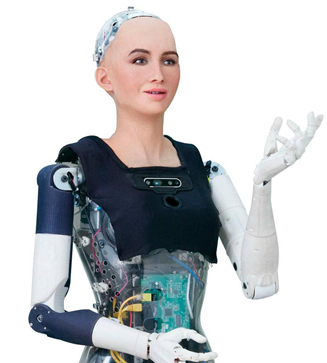
\includegraphics[width=0.3\linewidth]{Main/Chapter2/Images2/Robot-humanoideSophiaIA.png}
        \caption{Robot humanoide Sophia, IA \cite{robot_sofi}} 
        \label{f:Cap2_general_1}
    \end{figure}   
    
    La palabra robot fue usada por primera vez en el año 1921 en la obra de teatro R.U.R (Rossums Universal Robots, figura \eqref{f:Cap2_general_2}) creada por el escritor checo Karel Capek (1890 - 1939). El origen etimológico de la palabra es robota, que significa en checo trabajo forzado o esclavo. Posteriormente se emplea la palabra ``robótica'' en obras de ciencia ficción tales como: Yo Robot (1950) y Robots e imperio (1985) creadas por el escritor y profesor de bioquímica Isaac Asimov (1920-1992).
    
    \newpage
    
    \begin{figure}[htb]
        \centering
        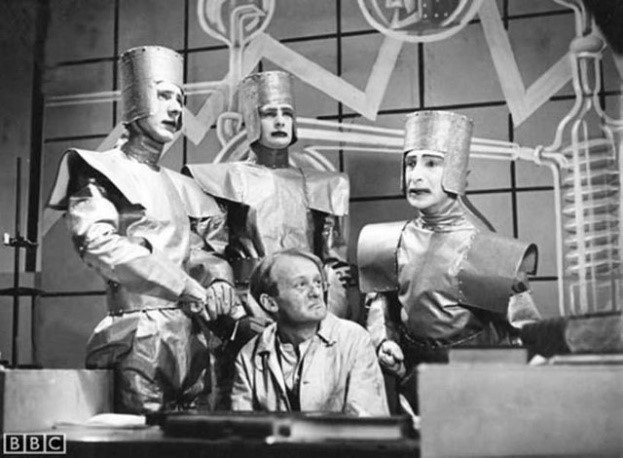
\includegraphics[width=0.6\linewidth]{Main/Chapter2/Images2/Obra-robots.jpg}
        \caption{Obra R.U.R (Robots Universal Rossum) creada por Karel Capek \cite{cap2_rur}}
        \label{f:Cap2_general_2}
    \end{figure}
    
    Hoy en día los expertos en el área de la robótica y automatización no han llegado a un acuerdo para una definición universal de la palabra robot. Es por esta razón que a continuación se presenta la descripción de un robot respecto al punto de vista de tres instituciones importantes:
    
    \begin{itemize}
    
        \item \textbf{Robot Institute of America (RIA)}: ``Un robot es un manipulador reprogramable multifuncional diseñado para mover material, partes, herramientas o dispositivos especializados a través de movimientos programados variables para el desarrollo de una variedad de tareas.''
        
        \item \textbf{Japanese Industrial Robot Association (JIRA)}: ``Un robot de un dispositivo con grados de libertad que puede ser controlado.''
        
        \item \textbf{International Federation of Robotics (IFR)}: ``Un robot es un mecanismo actuado programable en dos o más ejes con un grado de autonomía, que se mueva en su entorno para realizar tareas previstas.
        \textit{Nota 1: Un robot incluye el sistema de control y la interfase con el sistema de control.}\textit{Nota 2: La clasificación de robot industrial o robot de servicio se hace de acuerdo con la aplicación prevista.}''
        
    \end{itemize}
    
    A partir de las tres definiciones anteriores podemos concluir que un robot es un mecanismo programable o re-programable, capaz de interactuar con acciones independientes e inteligentes en un entorno especifico para realizar una variedad de tareas previstas.
    
    En este trabajo de título se estudia un robot de tipo delta. Esta compuesto por tres brazos conectados a una base fija y a otra móvil llamada efector. Al estar los tres brazos conectados a la misma base, la cinemática del robot es cerrada. Los brazos se accionan por medio de actuadores que generalmente son motores. En el efector final se encuentra generalmente herramientas para realizar tareas especificas.
    
    \newpage
\section{Historia de la robótica}
    
    Los robots son una gran noticia hoy en día gracias a las enormes mejoras que han provisto en diversas áreas de la vida de las personas y han abierto un nuevo capítulo en la interacción de humanos y robots para el futuro. Estas enormes mejoras han sido paulatinas, ya que la robótica tiene sus origenes hace miles de años. A continuación, se presentan algunos de los hitos registrados a través de la historia, que han ayudado a la robótica a convertirse en lo que es hoy.
    
 \begin{longtable}[c]{c m{12cm}}
     \label{tab:cap2_efemerides}\\

     \endfirsthead
    
     \hline
     \multicolumn{2}{|c|}{Continuación de la tabla \eqref{tab:cap2_efemerides}}\\
     \hline
     \endhead
    
     \hline
     \endfoot
    
     \hline
     \textbf{Año}  & \multicolumn{1}{c}{\textbf{Hito}}  \\\hline\hline
     \textbf{400 A.C} & El matemático y filósofo italiano Arquitas de Tarento hizo una paloma de madera que volaba. \\ \hline
     \textbf{10-70 D.C} & El matemático y científico griego Herón de Alejandría construyó diversos autómatas con forma de ave. Se le atribuye la invención de la primera máquina de vapor, conocida como “aeolipile” y la fuente de Herón. \\ \hline
     \textbf{1452 - 1519} & Leonardo Da Vinci diseño 2 autómatas, el primero consiste en un mecanismo que emulaba el movimiento humano vestido de armadura y el segundo un león mecánico \\ \hline
     \textbf{1947} & Primer manipulador eléctrico servo-controlado, por Goetz. \\ \hline
     \textbf{1952} & Primera máquina de control numérico, que se programa por un lenguaje simbólico Software. \\ \hline
     \textbf{1954} & El primer Robot: manipulador tipo brazo articulado que realizaba una secuencia de movimientos programables, desarrollado por George Devol. \\ \hline
     \textbf{1959} & George Devol conoció a Joseph Engelberger y juntos fundaron en 1960 la empresa Unimation dedicada a la fabricación de robot \\ \hline
     \textbf{1960} & Se produce el primer robot de configuración cilíndrica Versatran, por la compañía American Machine Foundry (AMF) \\ \hline
     \textbf{1961} & Unimation instala el primer Unimate en General Motors en los procesos de fundición; mientras que la Ford Motor Company instala un robot Versatran. \\ \hline
     \textbf{1963} & La compañía Fuji Yusoki Kogyo de Japón desarrolla el primer robot para aplicaciones de palletzing, llamado Palletizer. \\ \hline
     \multirow{2}{*}{\textbf{1968}} & Kawasaki adquiere los derechos de fabricación del Unimate en Japón. Comienza la fabricación e implementación de robots en las industrias de Japón. \\ \cline{2-2}
      & General Motors emplea baterías de robots en el proceso de fabricación de las carrocerías de los coches.\\ \hline
     \textbf{1970} & KUKA, empresa alemana, instala la primera línea de soldadura equipada con robots industriales. \\ \hline
     \textbf{1971} & Se funda la Japanese Industrial Robot Association (JIRA). \\ \hline
     \multirow{2}{*}{\textbf{1973}} & ASEA, empresa sueca, comercializa el primer robot industrial completamente eléctrico, IRB6. \\ \cline{2-2}
      & La empresa KUKA Robotics contruye el primer robot articulado electromecánicamente de 6 ejes nombrado FAMULUS.\\ \hline
     \multirow{2}{*}{\textbf{1974}} & Se funda el Robot Institute of America (RIA), actualmente llamado Robotic Industries Association.  \\ \cline{2-2}
             & Se introduce el primer robot industrial a España. \\ \cline{2-2}
             & Comienza en lenguaje de programación AL del que derivan otros robots posteriormente. \\ \hline
     \textbf{1978} & Unimation, con el desarrollo de Victor Scheinman, introduce el robot PUMA (Programmable Universal Machine for Assembly) con el lenguaje de programacion VAL (Victor’s Assembly Languaje). \\ \hline
     \textbf{1979} & A partir del desarrollo del profesor Hiroshi Makino de la Universidad de Yamanashi de Japón se produce el primer robot SCARA (Selective Compliance Assembly Robot Arm) a manos de Sankyo e IBM. \\ \hline
     \textbf{1980} & Fundación de la Federación Internacional de Robótica (IFR). \\ \hline
     \textbf{1981} & La compañía americana PaR Systems introduce el primer robot Gantry o de plataforma industrial. \\ \hline
     \multirow{2}{*}{\textbf{1984}} & Adept introduce el primer robot SCARA de accionamiento directo llamado AdeptOne. \\ \cline{2-2}
      &  ABB, empresa sueca formada a partir de ASEA, produce el IRB 1000, el robot ensamblador más rápido hasta la fecha. \\ \hline
     \textbf{1987} & Se constituye la Federación Internacional de Robótica con sede en Estocolmo. \\ \hline
     \textbf{1992} & Aparece el robot DELTA, diseñado por el científico suizo Reymond Clavel en su tesis de doctorado. \\ \hline
     \textbf{1994} & Motoman presenta el primer sistema de control de robots (MRC) que proporcionó el control sincronizado de dos robots hasta 21 ejes. \\ \hline
     \textbf{1998} & ABB, basándose en la estructura del robot Delta, desarrolla el Flex-Picker, considerador el robot de selección más rápido del mundo. \\ \hline
     \textbf{1999} & La compañía alemana Reis Robotics, integra una guía de rayo láser integrada dentro de sus brazos robóticos. \\ \hline
     \textbf{2004} & Motoman introduce un sistema de control robótico mejorado (NX100), que provee control sincronizado de cuatro robots hasta 38 ejes. \\ \hline
     \multirow{2}{*}{\textbf{2006}} & La compañía de automatización Comau de Italia presenta el primer Teach Pendant Inalámbrico (WiTP). \\ \cline{2-2}
        & KUKA presenta el primer robot de peso ligero (LWR) conformado por una estructura de aluminio. \\ \hline
     \textbf{2007} & Motoman lanza robots super rápidos de soldadura por arco, que reduce los tiempos de ciclo en un 15\% 
     \\ \hline
     \textbf{2009} &  ABB lanza el robot industrial multipropósito más pequeño, IRB120, que pesa solo 25kg y un alcance de 580mm. \\ \hline
     \textbf{2013} & KUKA presenta un robot diseñado para una colaboración segura humano-robot del área de trabaja llamado LBR iiwa “Leichtbauroboter intelligent industrial work assistant”, que cuenta con 7 ejes. \\ \hline
    \caption{Evolución de la robótica industrial}
 \end{longtable}
 
    El robot delta fue investigado e inventando en 1985 por el profesor Reymond Clavel (figura \eqref{f:Cap2_general_4}) y su equipo en el laboratorio de sistemas de robótica de la la École Polytechnique Fédérale de Lausanne (EPFL, Suiza). Ellos comenzaron la investigación del robot delta después de una visita a una fabrica de chocolate. El equipo de Clavel estaba buscando aplicaciones de mano de obra repetitivas para robots, y descubrieron que el empaque de bombones de chocolate era un candidato para este tipo de automatización de alta velocidad y baja carga útil. En ese mismo año se completo el prototipo de robot delta, el cual fue patentado. En 1987 la compañía suiza Demareux Robotics and Microtechnology compró una licencia del robot delta y comenzó la producción estos para la industria de empaquetamiento. En 1991 el Dr. Reymond Clavel presentó su tesis doctoral 'Conception d'un robot parallèle rapide à 4 degrés de liberté' y recibió el premio Golden Robot, Award patrocinado por ABB Flexible Automation, por su trabajo innovador y desarrollo del robot delta.


    \begin{figure}[htb]
        \centering
        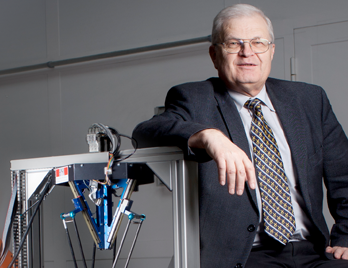
\includegraphics[width=0.36\linewidth]{Main/Chapter2/Images2/Reymond-Clavel-Robot-Delta.png}
        \caption{Reymond Clavel y el robot delta \cite{cap2_rey}}
        \label{f:Cap2_general_4}
    \end{figure}
    
    
\newpage    
    
\section{Clasificaciones de robots}
    
    \subsection{Clasificación por generación}
        \subsubsection{Primera generación}
            Robots manipuladores. Se caracterizan por programas de control fijos, relativamente sencillos de lazo abierto (sin retroalimentación). Son capaces de repetir operaciones previamente programadas en ellos, no pueden adaptarse al entorno, por lo que no deben existir perturbaciones externas. Por lo tanto, estos robots son los más adecuados en entornos industriales que realizan operaciones repetitivas.
        
        \subsubsection{Segunda generación}
            Robots de aprendizaje. Son adaptativos, pueden operar en entornos variables o parcialmente desconocidos. Estos robots ejecutan una serie de operaciones predefinidas, pero también pueden tener en cuenta los cambios en el entorno y modificar su rutina para realizar sus tareas. Imitan la secuencia de movimientos que ha sido ejecutada previamente por un operador humano. El operador realiza los movimientos requeridos mientras el robot le sigue y los memoriza con ayuda de sensores que recopilan datos.
        \subsubsection{Tercera generación}
            Robots con control sensorizado. Los robots cuentan con controladores (computadoras) que, usando los datos o la información recopilada de sus sensores, obtienen la habilidad de ejecutar las ordenes de un programa escrito en alguno de los lenguajes de programación que surgen a raíz de la necesidad de introducir las instrucciones deseadas en dichas máquinas. 
        \subsubsection{Cuarta generación}
            Robots inteligentes. Esta etapa se caracteriza por tener sensores mucho más perfeccionados que mandan información al controlador y la analizan mediante estrategias complejas de control. Incorpora inteligencia artificial totalmente. Esto permite una toma inteligente de decisiones y el control del proceso en tiempo real.

        \newpage
        
    \subsection{Clasificación por arquitectura o estructura}
        
        \subsubsection{Poli-articulados}
        La característica principal de este tipo de robots es la de ser sedentarios, aunque algunos tienen desplazamientos limitados. Tienen un espacio de trabajo limitado según uno o más sistemas de coordenadas y tienen un número limitado de grados de libertad. En la figura \eqref{f:Cap2_general_6} se muestra un ejemplo de estos robot, el cual esta encargado de labores de soldadura.
        
        \begin{figure}[htb]
            \centering
            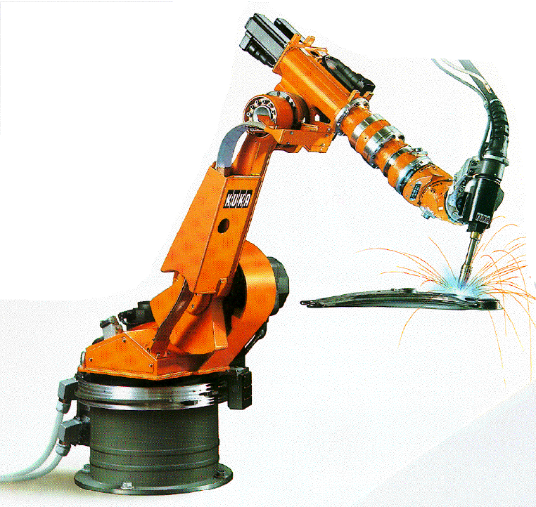
\includegraphics[width=0.35\linewidth]{Main/Chapter2/Images2/Robot-poliarticulado.png}
            \caption{Robot Poli-articulado \cite{ER4pc}}
            \label{f:Cap2_general_6}
        \end{figure}
        
        \subsubsection{Zoomórficos}
        La característica principal de este tipo de robot es que imitan los movimientos, desplazamientos y funciones de diversos tipos de seres vivos. Existen dos categorías de robots zoomórficos: no caminadores y caminadores. En la actualidad se encuentran en mayor cantidad los robots caminadores. Un ejemplo de estos ultimos es el robot que se aprecia en la figura \eqref{f:Cap2_general_7}, llamado 'Spot classic de Boston Dynamics'. Las aplicaciones de estos robots son esencialmente en áreas peligrosas tales como la exploración espacial, estudio de volcanes, fines militares e industrias nucleares. 
        
        \begin{figure}[htb]
            \centering
            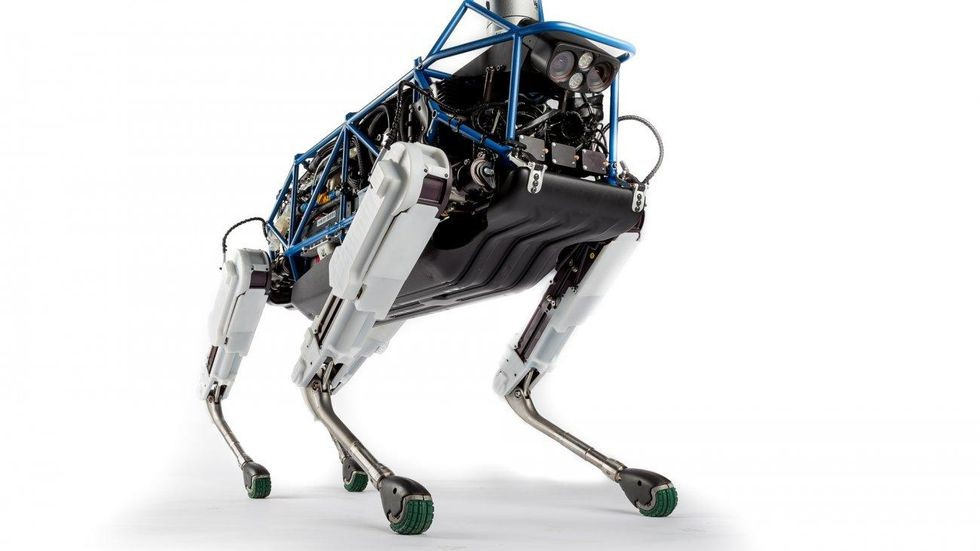
\includegraphics[width=0.48\linewidth]{Main/Chapter2/Images2/Robot-Zoomorico.jpg}
            \caption{Robot zoomórfico: Spot Classic (2015) de Boston Dynamics \cite{cap2_spotrobot}
 }
            \label{f:Cap2_general_7}
        \end{figure}
        
        \newpage
        
        \subsubsection{Móviles}
        Estos robots tienen una capacidad de desplazamiento amplia, basados en carros o plataformas y equipado de un sistema locomotor comúnmente de ruedas. Se desplazan por una trayectoria o camino por medio de un mando a distancia o guiándose a través de la información capturada por los sensores. Un ejemplo es el iRobot 510 PackBot mostrado en la figura \eqref{f:Cap2_general_8}, que se utiliza para realizar una variedad de misiones, incluida la eliminación de artefactos explosivos, manipulación de materiales peligrosos, etc.
        
        \begin{figure}[htb]
            \centering
            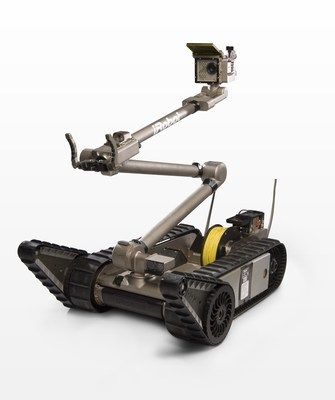
\includegraphics[width=0.27\linewidth]{Main/Chapter2/Images2/Robots-moviles.jpg}
            \caption{Robot móvil: 
            iRobot 510 PackBot.\cite{cap2_iRobot510}}
            \label{f:Cap2_general_8}
        \end{figure}
        
        \subsubsection{Androides}
        La particularidad de este tipo de robots es que son antropomorfos, en otras palabras, que tiene forma o apariencia humana y además imitan algunos aspectos de su conducta de manera autónoma. La mayor dificultad que tienen hoy en día los especialistas de este tipo de robots es simular el comportamiento cinemático del ser humano, llamado locomoción bípeda. La locomoción bípeda es la habilidad de los seres vivos de caminar sobre sus dos extremidades inferiores. Boston Dynamics tiene varios robots androides, entre los cuales se encuentra el robot Atlas visualizado en la figura.\eqref{f:Cap2_general_9}.
        
        \begin{figure}[htb]
            \centering
            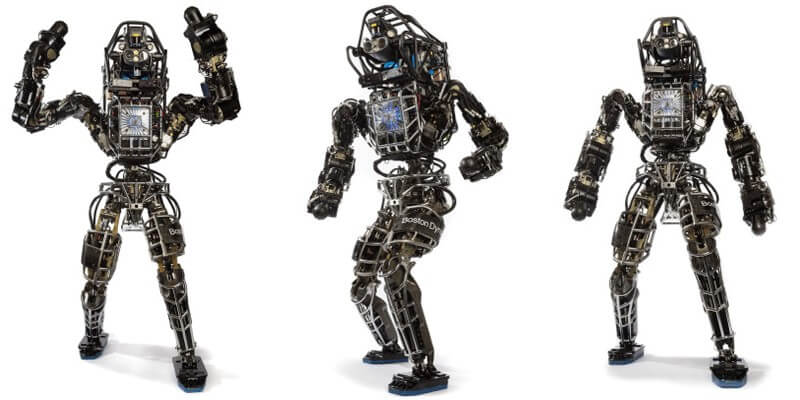
\includegraphics[width=0.65\linewidth]{Main/Chapter2/Images2/Robot-androide.png}
            \caption{Robot androide: Atlas de Boston Dynamics \cite{cap2_androide}}
            \label{f:Cap2_general_9}
        \end{figure}
        
        \newpage

    
    \subsection{Clasificación por su movimiento}
    
        \subsubsection{Robots articulados}
        
        Los robots articulados son unos de los tipos más comentados de robots industriales. Se asemejan a un brazo humano en su configuración mecánica. El brazo está conectado a la base con una articulación giratoria. Las articulaciones pueden ser paralelas u ortogonales entre sí. Los robots articulados que tienen seis grados de libertad son los robots industriales más utilizados, ya que el diseño ofrece la máxima flexibilidad.
        
        \begin{figure}[htb]
            \centering
            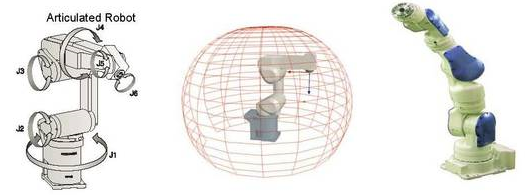
\includegraphics[width=1.0\linewidth]{Main/Chapter2/Images2/Robot-articulado.png}
            \caption{Robot Articulado \cite{cap2_class_mov}}
            \label{f:Cap2_segunMovimiento_articulado}
        \end{figure}
        
        \subsubsection{Robots cartesianos}
        
        Los robots cartesianos también se denominan robots rectilíneos y tienen una configuración rectangular. Estos tipos de robots industriales tienen tres articulaciones prismáticas para proporcionar movimiento lineal al deslizarse sobre sus tres ejes perpendiculares (X, Y, Z). 
        
        \begin{figure}[htb]
            \centering
            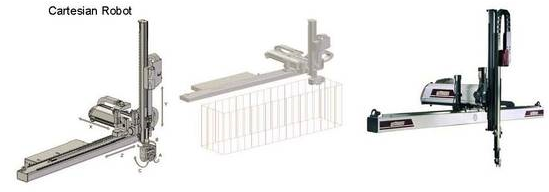
\includegraphics[width=1.0\linewidth]{Main/Chapter2/Images2/Robot-cartesiano.png}
            \caption{Robot Cartesiano \cite{cap2_class_mov}}
            \label{f:Cap2_segunMovimiento_cartesiano}
        \end{figure}
        
        \newpage

        
        \subsubsection{Robots SCARA}
        
        Los robots SCARA son los robots que pueden hacer 3 traslaciones más una rotación alrededor de un eje vertical. Los ejes rotativos se colocan verticalmente, y el efector final unido al brazo se mueve vertical. Por la configuración de los brazos de SCARA, son flexibles en los ejes XY y rígidos en el eje Z. Los robots SCARA se especializan en movimientos laterales y se utilizan principalmente para aplicaciones de ensamblaje. 
        
        \begin{figure}[htb]
            \centering
            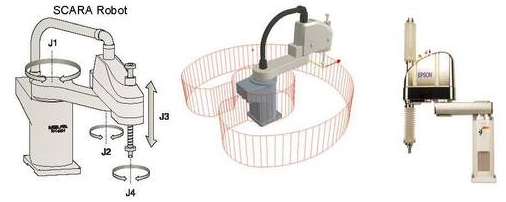
\includegraphics[width=0.9\linewidth]{Main/Chapter2/Images2/Robot-SCARA.png}
            \caption{Robot SCARA  \cite{cap2_class_mov}}
            \label{f:Cap2_segunMovimiento_scara}
        \end{figure}
        
        \subsubsection{Robots delta}
        
        Los robots delta también se les llama robots paralelos, ya que consiste en enlaces de unión paralelos conectados con una base fija común. Debido al control directo de cada junta sobre el efector final, el posicionamiento de este último se puede controlar fácilmente con sus brazos, lo que resulta un robot de operación de alta velocidad. El espacio de trabajo de los robots delta tienen forma de cúpula. Estos robots se utilizan generalmente para aplicaciones de pick and place.
        
        \begin{figure}[htb]
            \centering
            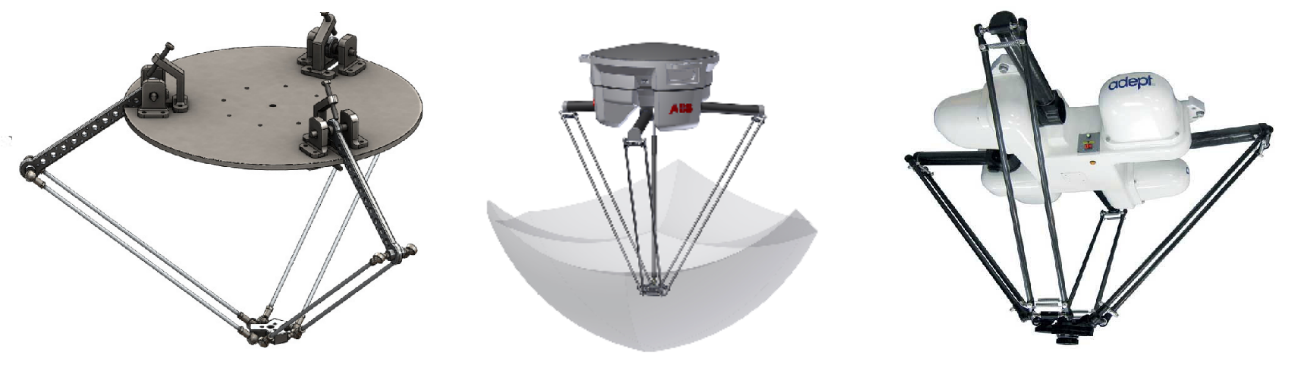
\includegraphics[width=0.9\linewidth]{Main/Chapter2/Images2/Robot-delta.png}
            \caption{Robot delta \cite{cap2_rdelta_1}\cite{cap2_rdelta_2}\cite{cap2_rdelta_3}}
            \label{f:Cap2_segunMovimiento_delta}
        \end{figure}
        
         \newpage

        
        \subsubsection{Robots cilíndricos}
        
        Los robots cilíndricos tienen al menos una junta giratoria en la base y al menos una junta prismática que conecta los enlaces. Estos robots tienen un espacio de trabajo cilíndrico con un eje pivotante y un brazo extensible que se mueve verticalmente y deslizándose. Por lo tanto, los robots con configuración cilíndrica ofrecen un movimiento lineal vertical y horizontal junto con un movimiento giratorio sobre el eje vertical.
        
        \begin{figure}[htb]
            \centering
            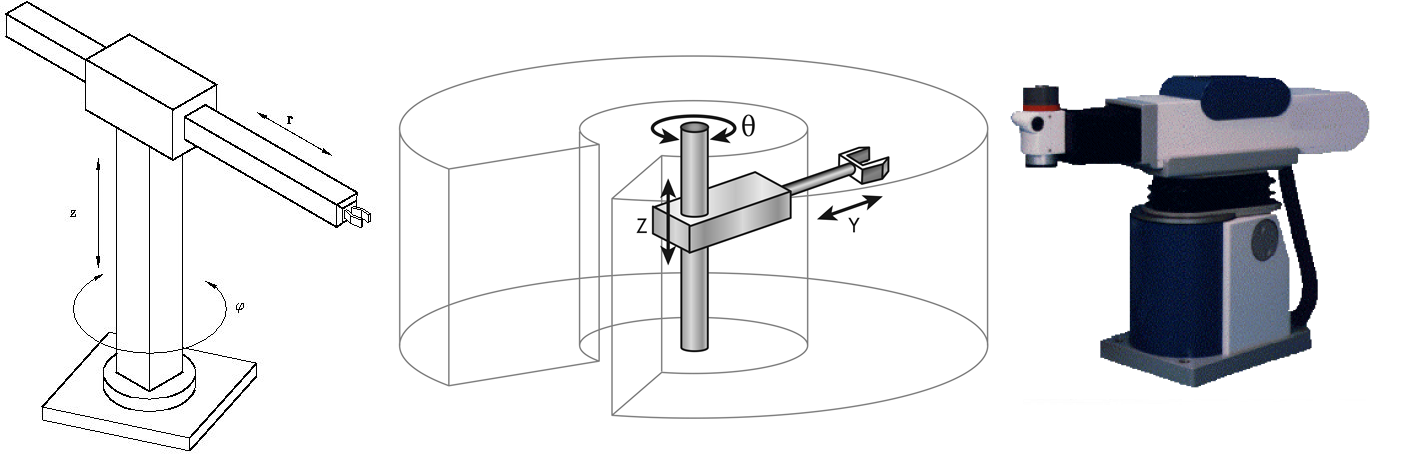
\includegraphics[width=1.0\linewidth]{Main/Chapter2/Images2/Robot-cilindrico.png}
            \caption{Robot cilíndrico \cite{cap2_class_polar_1}\cite{cap2_class_polar_cilin_2}\cite{cap2_class_polar_3}}
            \label{f:Cap2_segunMovimiento_cilindrico}
        \end{figure}
        
        \subsubsection{Robots polares}
        
        También llamados robots esféricos. En esta configuración el brazo está conectado a la base por una junta giratoria , una combinación de dos juntas rotativas y una junta lineal. Los ejes forman un sistema de coordenadas polares y crean una envoltura de trabajo de forma esférica.
        
        \begin{figure}[htb]
            \centering
            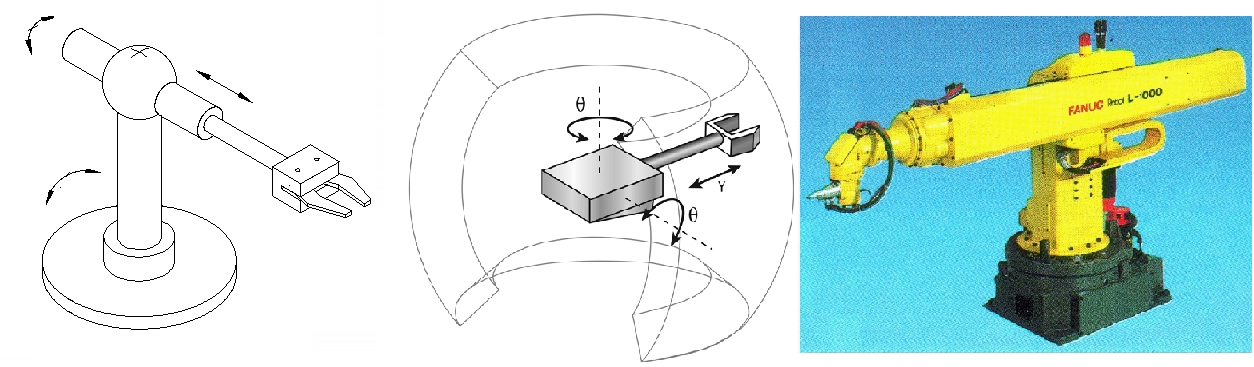
\includegraphics[width=1.0\linewidth]{Main/Chapter2/Images2/robot-polar.png}
            \caption{Robot polar \cite{cap2_class_polar_1}\cite{cap2_class_polar_cilin_2}  }
            \label{f:Cap2_segunMovimiento_polar}
        \end{figure}
    
                \newpage


\section{Estadísticas y aplicaciones}

    Muchos tipos de actividades en los sectores industriales tienen el potencial técnico para ser automatizados. Según el reporte ``El potencial técnico para la automatización en los EE. UU'' de McKinsey Company en enero del 2017, el 50\% de los trabajos realizados por humanos hoy son vulnerables al reemplazo por robots. Eso podría equivaler a una pérdida de \$15 billones dólares en salarios en todo el mundo y \$2.7 billones de dólares en los EE. UU. Esto puede ocurrir por completo entre los años 2035 -2055 aproximadamente. 
    
    En la práctica, la implementación de la automatización en nuestro mundo dependerá de más que solo la viabilidad técnica. Existen cinco factores:

        \begin{enumerate}
           \item {Viabilidad técnica.}
            \item {Costos para automatizar.}
            \item {La relativa escasez, las habilidades y el costo de los trabajadores de que otro modo podrían realizar la actividad.}
           \item {Beneficios de la automatización más allá de la sustitución del costo laboral.}
            \item {Consideraciones regulatorias y de aceptación social.}
    \end{enumerate}
    
    \begin{figure}[h]
        \centering
        
\includegraphics[width=0.2\linewidth]{Main/Chapter2/Images2/LOGOMCKINSEY.jpg}
        \caption{Logo de McKinsey Company \cite{mckinsey}}
        \label{f:Cap2_general_potencial_automatizacion_11}
    \end{figure}
    
    Según la figura \eqref{f:Cap2_general_potencial_automatizacion}, las actividades más automatizables son las que gran parte del tiempo implican realizar actividades físicas u operar maquinaria en un entorno predecible. Los trabajadores llevan a cabo acciones específicas en entornos conocidos donde los cambios son relativamente fáciles de anticipar. Dado que las actividades físicas predecibles ocupan un lugar destacado en sectores como la fabricación, el servicio de alimentos y el alojamiento y la venta minorista, estas son las más susceptibles a la automatización basadas solo en consideraciones técnicas.
    
    
    \begin{enumerate}
        \item \textbf{El sector de servicios}: El alojamiento y servicio de alimentos, donde casi la mitad de todo el tiempo de trabajo implica actividades físicas predecibles y la operación de maquinaria, incluida la preparación, la cocina o el servicio de alimentos; limpieza de áreas de preparación de alimentos; preparar bebidas frías y calientes; y la recolecta platos sucios. 
        \item \textbf{En la manufactura o producción}: Las actividades van desde el envasado de productos hasta la carga de materiales en equipos de producción, desde soldadura hasta mantenimiento de equipos.
        \item \textbf{El comercio minorista}: Los minoristas pueden aprovechar, por ejemplo, la gestión de existencias y la logística eficiente, impulsada por la tecnología. Los objetos de embalaje para el envío y almacenamiento de mercancías se encuentran entre las actividades físicas más frecuentes en el comercio minorista y tienen un alto potencial técnico para la automatización.
    \end{enumerate}

    \begin{figure}[h]
        \centering
        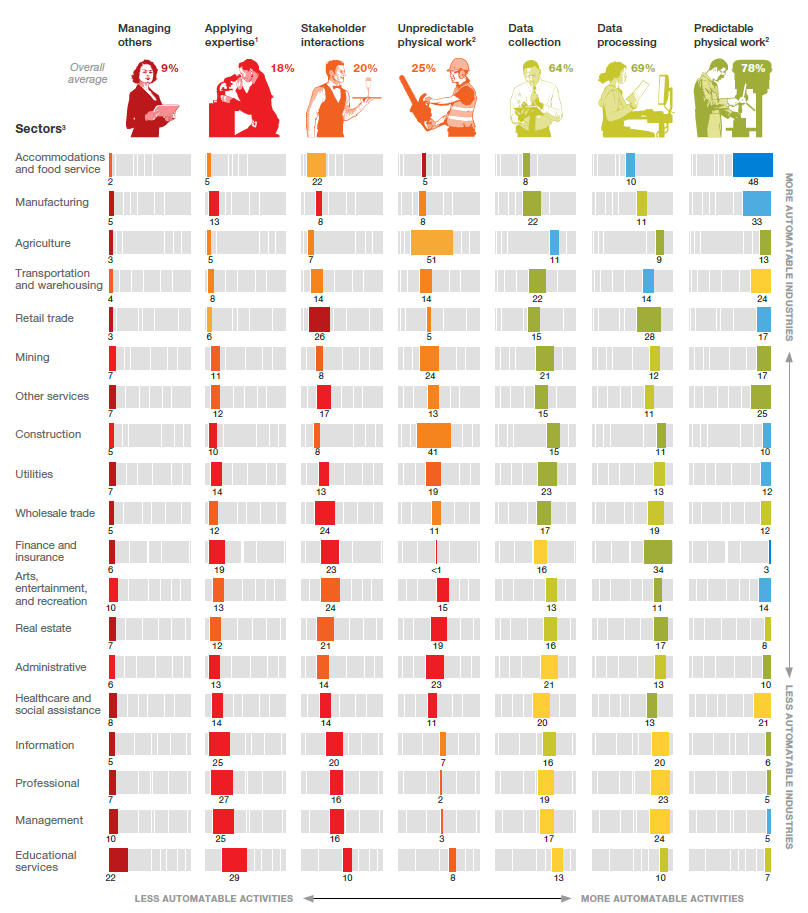
\includegraphics[width=0.97\linewidth]{Main/Chapter2/Images2/potencial-automatisacion.png}
        \caption{El potencial técnico para la automatización en los EE. UU. (McKinsey’s Company 2017) \cite{mckinsey_jobs}}
        \label{f:Cap2_general_potencial_automatizacion}
    \end{figure}
  
      \newpage
  
    Carl Benedikt Frey y Michael A. Osborne en el año 2013 publicaron su paper ``El futuro del empleo: ¿Cuán susceptibles son los trabajos para la computarización?” \cite{FREY2017254}. El efecto que causo en la población que leyó esta publicación, fue de dudas e incertidumbres, sin embargo, el reporte de la empresa McKinsey Company del 2017 mostrado anteriormente refuerza el trabajo realizado por el economista y por el profesor de machine learning. En la figura \eqref{f:Cap2_general_distribucion_empleo} se visualiza la probabilidad de computarización del trabajo por categorías. Se aprecia que el 47\% de los trabajos corren un alto riesgo de ser computarizados (probabilidad mayor a 70\%).
    
    \begin{figure}[htb]
        \centering
        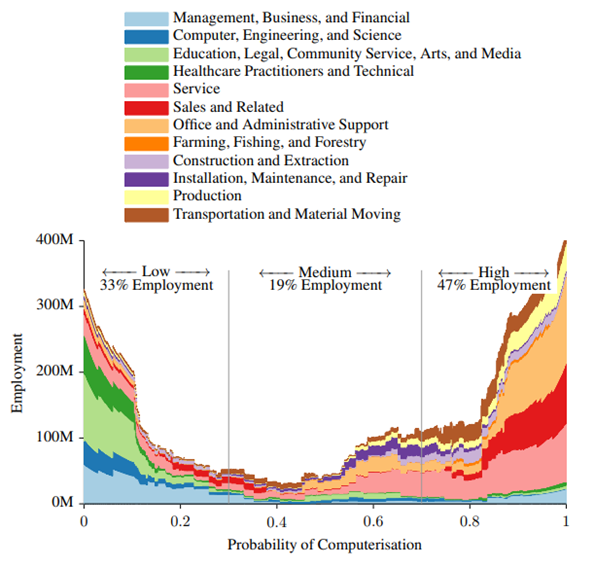
\includegraphics[width=1\linewidth]{Main/Chapter2/Images2/distribucion-del-empleo.png}
        \caption{La distribución del empleo ocupacional de BLS (Oficina de estadísticas laborales) 2010 sobre la probabilidad de computarización, junto con la participación en las categorías de probabilidad baja, media y alta. El área total bajo todas las curvas es igual al empleo total de los EE.UU \cite{FREY2017254}.}
        \label{f:Cap2_general_distribucion_empleo}
    \end{figure}
    
        \newpage


    Acerca del tamaño y crecimiento del mercado de robots industriales, se puede decir que pocos han mostrado un crecimiento tan fuerte y sostenido en la última década. La figura \eqref{f:Cap2_general_envios_anuales} reafirma este crecimiento. En los últimos años, las instalaciones anuales aumentaron en un 19\% CAGR, lo que resultó en 422,271 nuevas instalaciones globales en 2018, por un valor de USD 16,5 mil millones. Esto fue solo para el hardware robótico, mientras que el software / servicios y el hardware periférico ascendieron aproximadamente al mismo valor cada uno. A finales de 2018, el stock operativo global total de robots fue de 2.439.543. Asia es el motor de crecimiento detrás de estos números (dos de cada tres nuevas instalaciones robóticas ocurren en Asia), con China a la cabeza (aumentando el stock operativo de robots en casi un 30\% interanuales los años pasados). Europa y América se están quedando un poco atrás. 
    \begin{figure}[H]
        \centering
        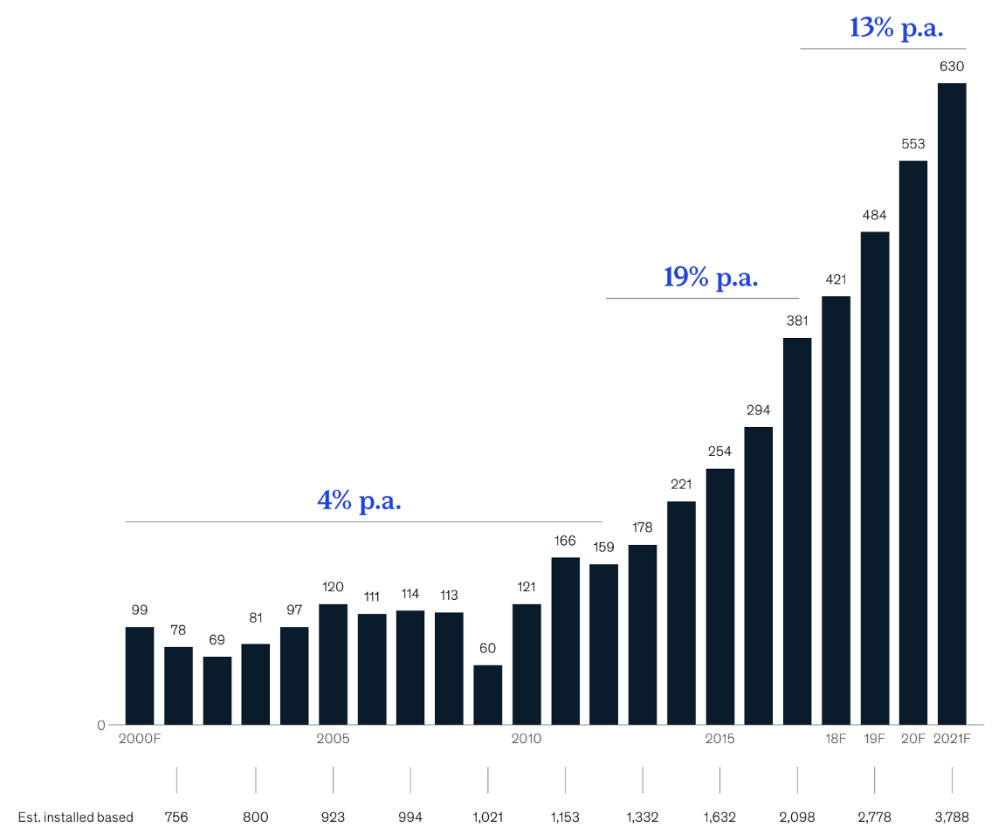
\includegraphics[width=0.67\linewidth]{Main/Chapter2/Images2/envios-anuales-robots.png}
        \caption{Envíos anuales (en miles) de robots industriales en todo el mundo \cite{growth_Insights}.}
        \label{f:Cap2_general_envios_anuales}
    \end{figure}
    Además del rápido crecimiento, lo más emocionante de la robótica es el impacto fundamental que tendrá en nuestras vidas futuras, librándonos potencialmente de la mayor parte del trabajo manual. A pesar de una percepción comúnmente diferente, incluso en industrias “altamente automatizadas” como la automotriz, el grado promedio de automatización (número de tareas automatizadas / número de tareas totales) en el ensamblaje final es solo alrededor del 8-10\%. Y la mayoría de las otras industrias están muy por debajo de eso. Por otro lado, generalmente se estima que hasta el 85\% de todas las tareas son 'automatizables'. Escalar esta curva de automatización ofrece una gran oportunidad para aumentar la productividad y el bienestar global, si nosotros, como sociedad, podemos compartir sus beneficios por igual.
    
            \newpage
    
    Los robots siguen siendo esencialmente demasiado caros y demasiado 'estúpidos', lo que permite muy pocas áreas de aplicación rentables. Pero nos enfrentamos a una tormenta perfecta de inventos innovadores que pronto desbloquearán un punto de inflexión, donde la robótica será significativamente más barata y más versátil que la mayoría del trabajo manual.
    
     A pesar de no incluir datos de los últimos años, la figura \eqref{f:Cap2_general_solicitud_patentes} muestra las solicitudes anuales de patentes de la UE y los EE. UU. para tecnologías de fabricación avanzadas (incluida la robótica) solo han comenzado a despegar en la última década. A medida que estos esfuerzos exponenciales de I + D alcancen la madurez comercial, se desbloqueará una ola sin precedentes de nuevos (y rentables) casos de uso de robótica. 
     
    \begin{figure}[H]
        \centering
        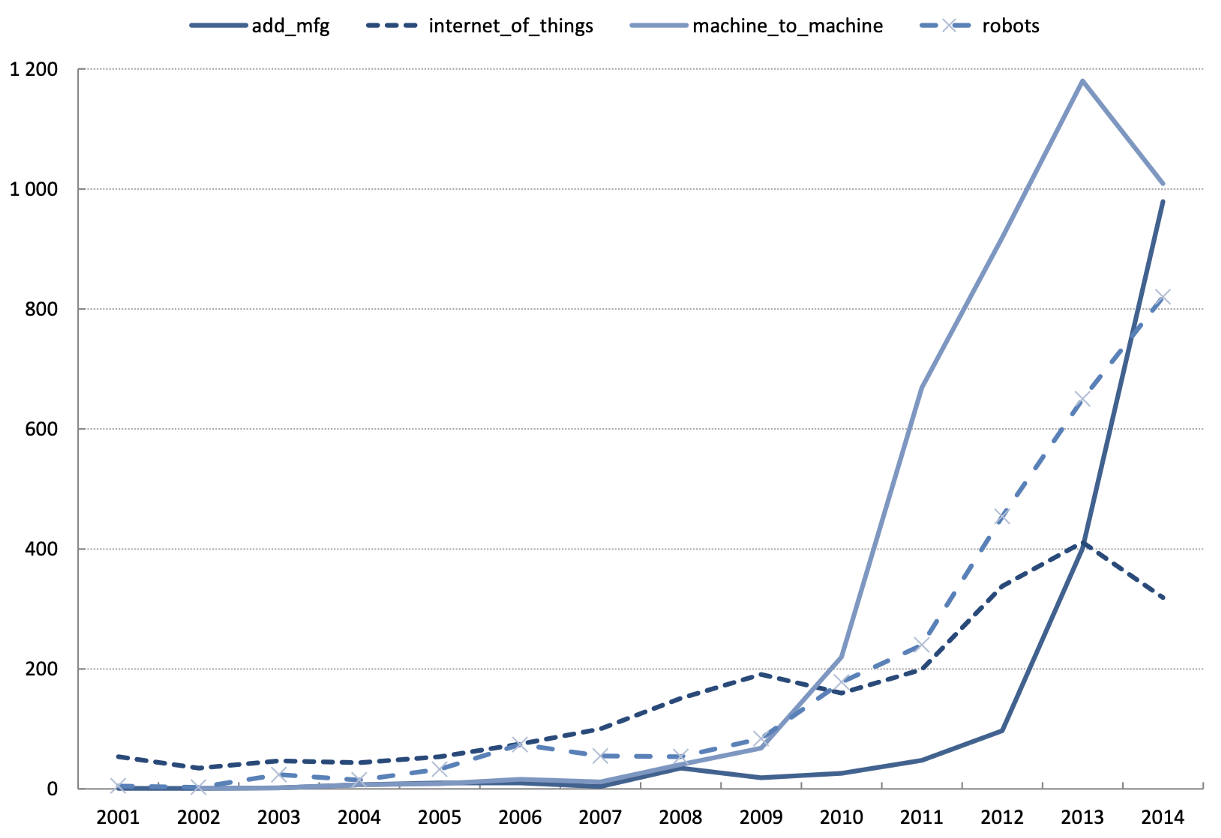
\includegraphics[width=1\linewidth]{Main/Chapter2/Images2/solicitud-patentes.png}
        \caption{Solicitudes de patentes anuales para tecnologías de fabricación avanzadas específicas \cite{dd98ff58}}
        \label{f:Cap2_general_solicitud_patentes}
    \end{figure}

 
    Las empresas que están innovando en el área de robótica buscan solucionar problemáticas para que sea más accesible a la mayor cantidad de personas, para este propósito desarrollan nuevas tecnologías para minorar los costos o hacer más flexible la robótica. Se pueden dividir en categorías las principales áreas de innovación en robótica, tales como se presentan en la figura \eqref{f:Cap2_general_empresas_robotica}:

    \newpage
    
    \begin{figure}[H]
        \centering
        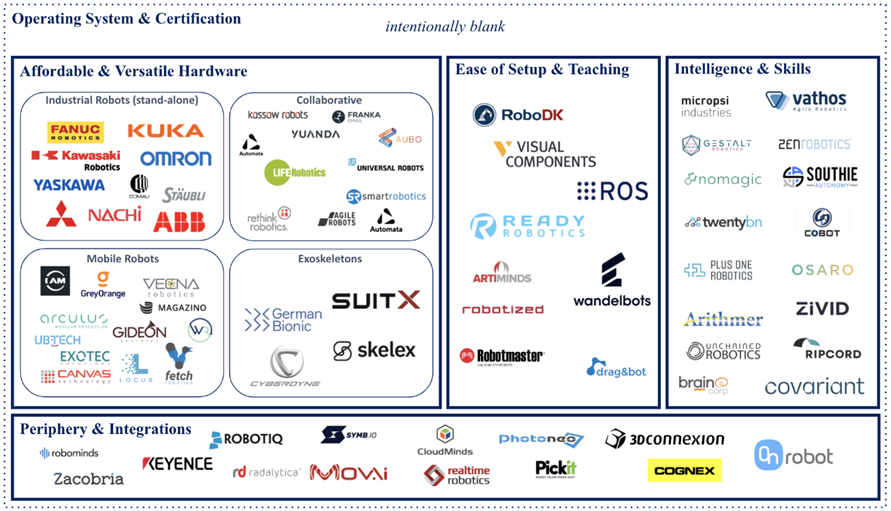
\includegraphics[width=1.0\linewidth]{Main/Chapter2/Images2/empresas-robotica.png}
        \caption{Mapa del mercado de robótica industrial \cite{pauventures}}
        \label{f:Cap2_general_empresas_robotica}
    \end{figure}
    
    \begin{itemize}
        \item{ \textbf{Hardware asequible y versátil}: en la última década, los costos promedio de una instalación robótica se han reducido aproximadamente en un 40\%, mientras que su productividad ha aumentado aproximadamente un 5\% por año. Se necesitarán nuevos modelos de negocio para ayudar a fomentar la adopción del mercado (por ejemplo, ``robot como servicio'' o modelos de alquiler). Al mismo tiempo, las capacidades mecánicas y las propiedades físicas deben mejorar (menos peso, mayor alcance, mayor velocidad, mejor modularidad, mejores sistemas de seguridad, etc.).}
        \item{ \textbf{Facilidad de configuración y enseñanza}: hoy en día, alrededor del 70\% de los costos totales de vida útil de una celda robótica son generados por servicios relacionados con la configuración, la programación y la enseñanza. Por lo general, esto lo realizan una gran cantidad de integradores de sistemas de tamaño pequeño a mediano, y demoran semanas o meses en configurar, programar y certificar una nueva aplicación de robótica. Por lo tanto, aquí no solo enfrentamos un problema de costos y tiempo, sino también un desafío de inflexibilidad. }
        \item {\textbf{Inteligencia y habilidades}: después de codificar dolorosamente una aplicación robótica, sigue siendo en gran medida rígida e inflexible. Si, por ejemplo, la forma o la posición de las piezas que va a recoger un robot cambian con el tiempo, en la mayoría de los casos esto significaría ``fin del juego'' para un robot industrial. }
    \end{itemize}

\newpage

    \begin{itemize}
        \item{ \textbf{Periferia e integraciones}: Una celda robótica siempre comprende elementos de hardware adicionales como pinzas y herramientas, sistemas de transporte, sistemas de seguridad, cámaras 2D y 3D, etc. La mayoría de estos sistemas periféricos provienen de diferentes proveedores, no tienen interfaces estándar y no se comunican fácilmente entre ellos. La creación de estándares y la modularización es clave para permitir una experiencia plug \& play ``consumida'' en diferentes proveedores de sistemas.}
        \item{ \textbf{Sistema operativo y certificación}: Hoy en día, no existe un ``MS Windows'' para la robótica industrial, que permitiría que todas las partes individuales que arman un robot se comuniquen entre sí. A pesar de algunos esfuerzos de código abierto, como ROS2 (Robotics Operating System 2), todavía no se ha encontrado ningún estándar de software real de la industria.}
    \end{itemize}
    %  arte
  \chapter{Arquitectura de un robot delta}\label{CAP3}

El tema que trata este capitulo es acerca de la descripción del robot delta y las herramientas que se utilizan para la solución de la problemática de la modelación cinemática y dinámica. Inicialmente se explica de forma general el funcionamiento y la estructura básica de un robot delta, con el fin de que el lector de esta tesis entienda lo complejo que es crear un robot por la gran variedad de áreas que lo componen. Luego se muestra gráficamente y se describen las partes mecánicas o piezas físicas con que esta estructurado el robot. Posteriormente se presenta el funcionamiento y los componentes del middleware ROS, que es el encargado de controlar y ordenar la lógica de la modelación cinemática y dinámica. Enseguida se enseña la herramienta de ROS llamada Rviz, que es la encargada de la visualización del robot. Finalmente se muestra el sofware que comprueba la modelación dinámica del sistema, llamado ADAMS.

\section{Funcionamiento general}

La principal tarea de un robot es ir de un punto a otro para realizar una determinada acción. Para realizar dicha acción se debe pasar por una serie de pasos complejos con el fin de asegurar una ejecución exitosa. Con la intención de explicar brevemente los pasos a seguir para lograr dicho objetivo, en la figura \eqref{f:Cap3-1_diagrama_de_flujo_robot_accion} se muestra un ejemplo básico de un robot delta accionado por motores paso a paso por medio de un diagrama de flujo.\\

Los pasos del diagrama de flujo son los siguientes:

\begin{enumerate}
    \item Definir los puntos de inicio y final de la trayectoria del robot.
    \item Elegir el tipo de trayectoria: posiciones, velocidades y aceleraciones impuestas.
    \item Comprobar la cinemática para obtener la trayectoria angular de los motores .
    \item Transformación de la trayectoria cartesiana a la trayectoria en el espacio articular de los actuadores.    
    \item Comprobar dinámica para asegurar que la trayectoria impuesta no dañe los componentes del robot y los motores.
    \item Traducción de trayectoria en el espacio articular a pulsaciones que entiendan los drivers de cada motor.
    \item Envío de pulsos al driver de los motores por medio de un controlador.
    \item Envío de pulsos del driver hacia los motores paso a paso.
\end{enumerate}

    \begin{figure}[h]
        \centering
        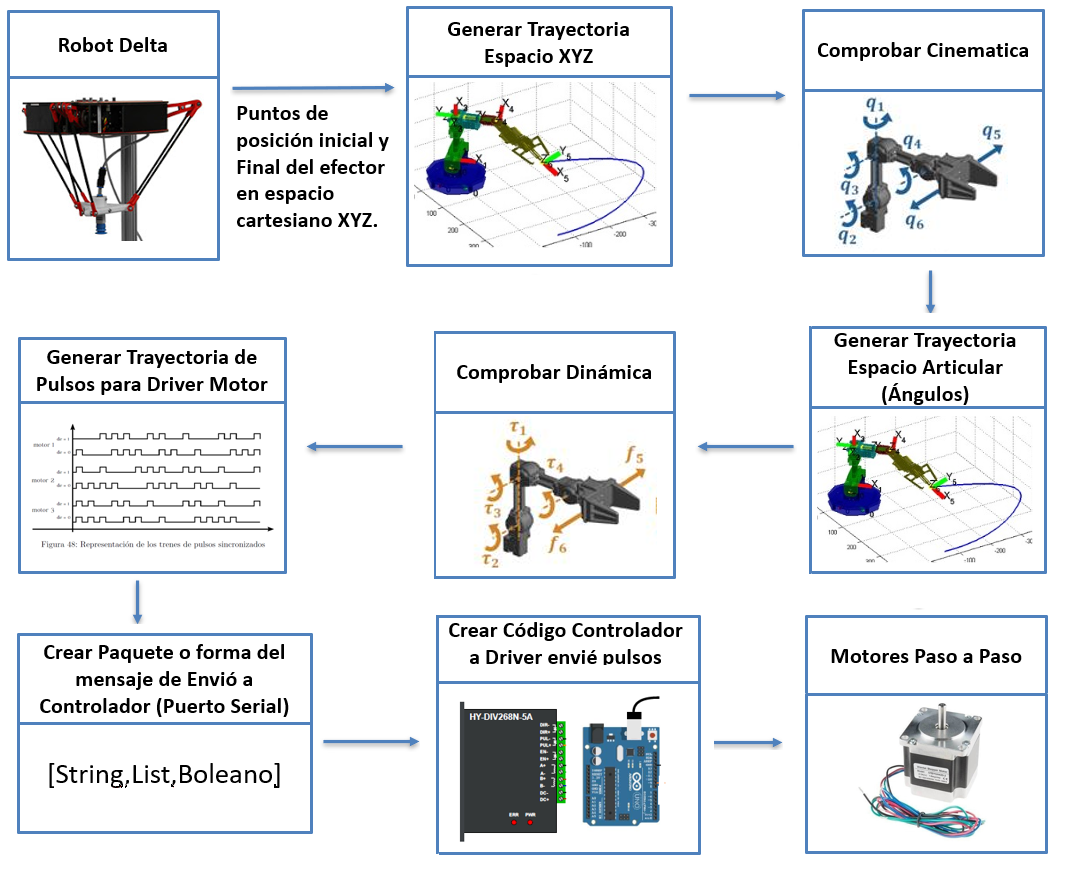
\includegraphics[width=1\linewidth]{Main/Chapter3/Images3/3-1/diagrama-de-flujo-robot.png}
        \caption{Ejemplo de diagrama de flujo de tareas que realiza un robot delta para realizar una trayectoria especifica}
        \label{f:Cap3-1_diagrama_de_flujo_robot_accion}
    \end{figure}
        \newpage
        
\section{Estructura de un robot delta}
%00X0 : reordenar los títulos del cap al diagrama de abajo en formato general, y luego explicar los software específicos para nosotros

    El robot delta puede ser subdivido por categorías de acuerdo al grupo estructural al que pertenezcan. Estas categorías facilitan la generación de conceptos para cada grupo de manera independiente, como se ilustra en la figura \eqref{f:Cap3-2_esquema_arquitectura_robot_delta}.
    
    \begin{figure}[h]
        \centering
        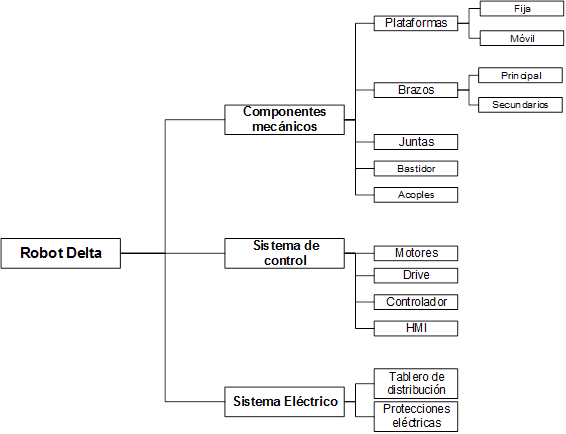
\includegraphics[width=0.8\linewidth]{Main/Chapter3/Images3/3-2/esquema-categorias-estructura.png}
        \caption{Descomposición estructural del robot delta \cite{Robot_parelelo_tipo}}
        \label{f:Cap3-2_esquema_arquitectura_robot_delta}
    \end{figure}
    
    \begin{enumerate}
        \item{ \textbf{Los componentes mecánicos}: son todas las piezas físicas que componen el robot delta. Es muy importante la elección del tipo de juntas a elegir ya que restringen el espacio de trabajo del robot delta. Por otro lado, se pueden optimizar las dimensiones de los largos de los brazos y antebrazos del robot con respecto a la energía suministrada a los motores y al espacio de trabajo.}
        \item{\textbf{El sistema de control}: es todo lo que está relacionado con el control del movimiento del robot delta. Los motores, que mueven los brazos del robot delta, deben controlarse a través de drivers por la complejidad de su accionamiento.}
        \item{ \textbf{El controlador}: este puede tener el algoritmo que crea las trayectorias cartesianas para realizar el movimiento del robot de un punto a otro. El HMI es la interfaz que ayuda a visualizar si el movimiento deseado del robot es correcto antes de que se realice.}
        \item{   \textbf{Los componentes eléctricos}: son todo lo relacionado con la electricidad como fuentes de poder para los motores, cables de conexión, fusibles, switch, etc.}
    \end{enumerate}

        \newpage

    Con el propósito de crear un modelo de un robot delta como guía para el desarrollo de este trabajo, se crea una arquitectura con ejemplos reales, enfocado solo en el sistema de control, tal como se presenta en la figura \eqref{f:Cap3-2_esquema_sistema_control} donde:

    \begin{figure}[h]
        \centering
        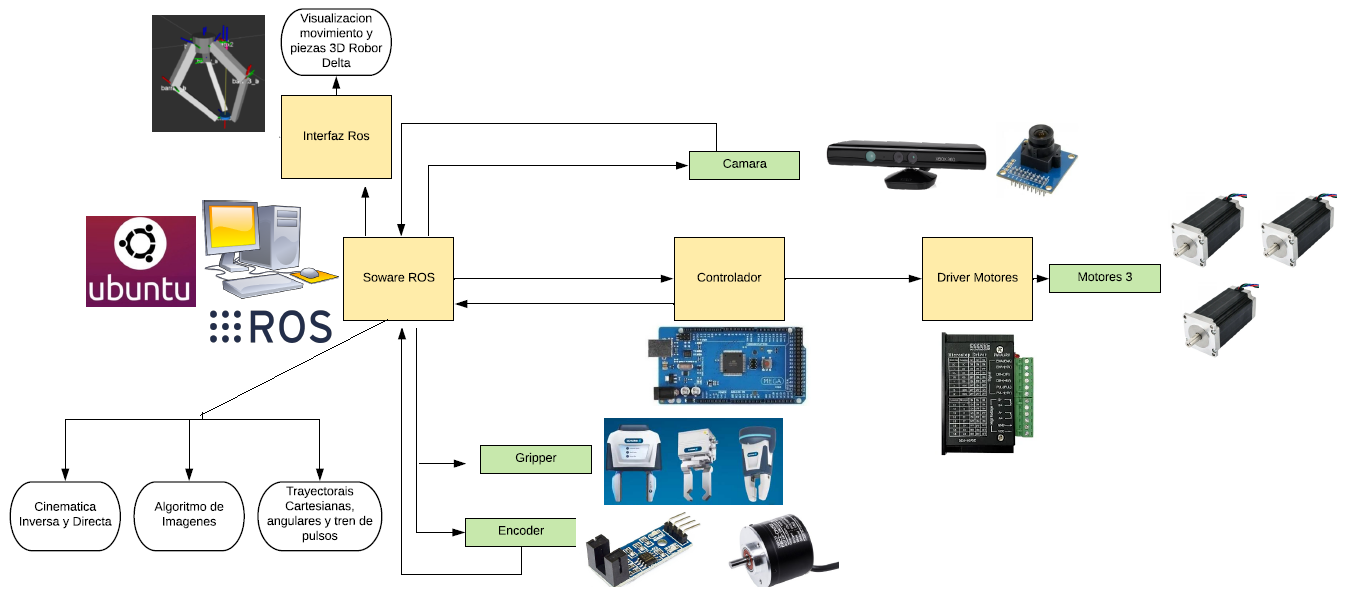
\includegraphics[width=1\linewidth]{Main/Chapter3/Images3/3-2/sistema-de-control.png}
        \caption{Ejemplo de el sistema de control de un robot delta}
        \label{f:Cap3-2_esquema_sistema_control}
    \end{figure}
    
    \begin{itemize}
        \item \textbf{Software ROS:} Es el encargado de procesar y ejecutar los algoritmos de cinemática y dinámica del robot delta. Además, controla el envió, la recepción y el procesamiento de datos de los sensores y del controlador.
        \item \textbf{Controlador:} Realiza la conversión de la trayectoria cartesiana o angular a un formato compatible con el driver de los motores. Se puede utilizar Arduino, Raspberry Pi, etc.
        \item \textbf{Rviz:} Interfaz gráfica que simula las trayectorias y las partes mecanicas del robot.
        \item \textbf{Kinect:} Sensor RGB y de profundidad que controla la posición del robot creando un lazo cerrado.
        \item \textbf{Actuadores:} Motores paso a paso controlados por drivers.
        \item \textbf{Encoder:} Sensor de posición y velocidad angular que controla la precisión los actuadores, creando un lazo cerrado.
        \item \textbf{Gripper:} Pinzas que sujetan los objetos.
    \end{itemize}
    
     En esta tesis solo abarca lo relacionado con ROS y la interfaz gráfica Rviz.
    
    \newpage

    
\section{Partes mecánicas}
    Con el objetivo de describir el robot delta, en esta sección se presenta un resumen del capítulo 2 de la tesis doctoral del ingeniero mecánico Reymond Clavel, el creador de este mecanismo, realizada en École Polytechnique Fédérale de Lausanne \cite{Clavel:31403}. 

    
    \subsection{Investigación}
    El primer objetivo que busca Reymond Clavel es el movimiento de piezas ligeras a gran velocidad en robots, ya que las aplicaciones objetivo de su investigación se encuentran en los campos del envasado en el sector alimentario, despaletización y paletización al inicio o al final de una línea de montaje, el montaje de componentes mecánicos, etc. Para todas estas operaciones se requiere un ritmo alto de producción/operación y los contactos de la industria de Clavel confirmaban esa tendencia en aquellos tiempos.
    
    Para lograr una alta tasa de trabajo durante operaciones que requieren carreras reducidas, el robot debe tener esencialmente una capacidad de aceleración y frenado; esta propiedad se obtiene mediante el uso de potentes actuadores debajo y mediante una estructura móvil muy ligera. Un estudio anterior de robot rápido del Clavel hizo posible probar el uso de gatos hidráulicos a alta velocidad con masas relativamente pesadas, pero por razones de coste y limpieza no querían utilizar energía hidráulica, por lo que lo llevo al enfoque de una ``estructura móvil y ligera``.
    
    La búsqueda de una función general de un robot delta se basó en una metodología enseñada en estudios de microtecnología en EPFL. Según la metodología antes mencionada, el primer paso de la cadena de costos consiste en definir la función global del producto considerado. La representación de la función se muestra en la figura \ref{f:Cap3-3_caja_negra_reymond}, mediante una caja negra con las diferentes entradas y salidas.
    
    \begin{figure}[htb]
        \centering
        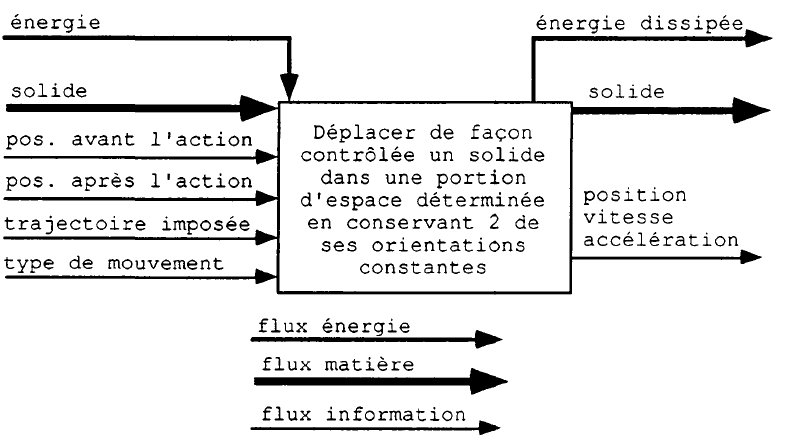
\includegraphics[width=0.75\linewidth]{Main/Chapter3/Images3/3-3/caja-negra-reymond.png}
        \caption{Representación de la función general del robot \cite{Clavel:31403}}
        \label{f:Cap3-3_caja_negra_reymond}
    \end{figure}
    
    \newpage
    
    \subsection{Elección del concepto ``Delta``}
    El catálogo de soluciones del anexo A2.2 de la tesis doctoral \cite{Clavel:31403} presenta 18 tipos de soluciones principales de la estructura de un robot delta que permiten mantener constantes 2 orientaciones de un sólido. La figura \eqref{f:Cap3-3_soluciones_interesantes_catalogo} muestra las soluciones más interesantes para el objetivo previsto. 

     \begin{figure}[htb]
        \centering
        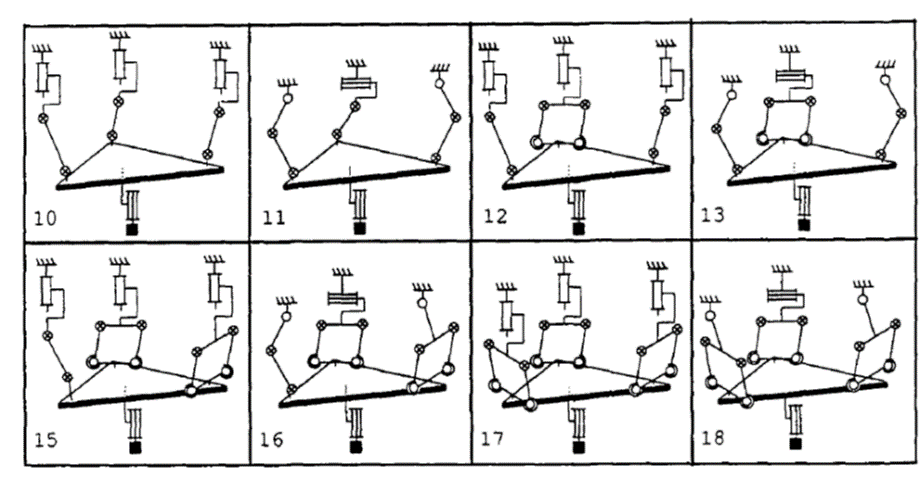
\includegraphics[width=0.85\linewidth]{Main/Chapter3/Images3/3-3/soluciones-interesantes.png}
        \caption{Extracto de las soluciones del catálogo ubicado en el apéndice A.2.2  \cite{Clavel:31403}}
        \label{f:Cap3-3_soluciones_interesantes_catalogo}
    \end{figure}
 
      \begin{figure}[htb]
        \centering
        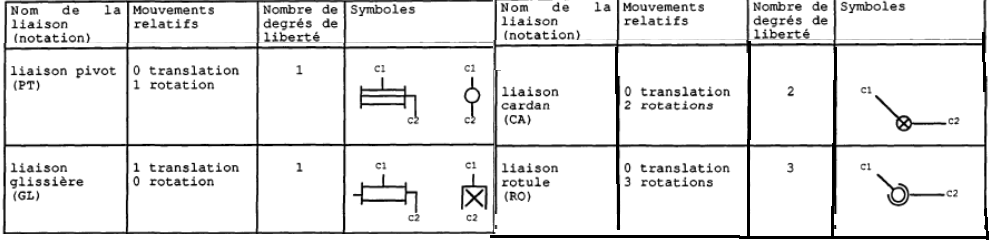
\includegraphics[width=0.8\linewidth]{Main/Chapter4/Images4/juntas.png}
        \caption{Nombre, movimiento relativo. grados de libertad y símbolos de juntas dibujadas en la figura  \eqref{f:Cap3-3_soluciones_interesantes_catalogo}  \cite{Clavel:31403}}
        \label{f:Cap3-3_soluciones_interesantes_catalogo_JUNTAS}
    \end{figure}
 
 Entre estas 18 soluciones, Reymond conserva aquellas que tienen las siguientes particularidades:   
    \begin{itemize}
        \item El movimiento en el espacio (con tres grados de libertad) es proporcionado por el tres actuadores fijos a la base fija. Las soluciones 10 a 13 y 15 a 18 de la figura \eqref{f:Cap3-3_soluciones_interesantes_catalogo} cumplen esta condición.
        \item Los actuadores son del tipo giratorio. Las soluciones 11, 13, 16 y 18 cumplen esta condicion.
        \item La estabilidad del órgano terminal está asegurada por una mayoría de elementos que trabajan en tensión-compresión más que en torsión. Finalmente se adopta la solución numero 18.
    \end{itemize}
    

    
        \newpage
    
    \subsection{Descripción del concepto ``Delta'' y sus componentes}
    La figura \eqref{f:Cap3-3_esquema_principal_robot_delta} sirve de apoyo para la descripción del robot delta y su funcionamiento. Este es un robot con cuatro grados de libertad. Se compone principalmente de una ``base fija'' (1) integrada a un marco de soporte de la instalación y una placa móvil (5); el nombre que se le da a esta última pieza es ``góndola'' (nacelle en frances). La conexión entre la base fija (1) y la góndola (5) se realiza mediante tres cadenas cinemáticas, cada una de ellas está formado por un ``brazo'' (2) montado en una articulación pivotante sobre la base fija y 2 ``barras paralelas'' (3) provistas cada una de una articulación (4) en cada extremo. El conjunto anterior formado por 2 barras paralelas y 2 elementos de conexión al brazo y a la góndola, se denomina ``paralelogramo''. Cada brazo (2) es impulsado por un ``motor de brazo'' (7) que, con mayor frecuencia, adopta la forma de un conjunto de motor reductor de sensor. La ``Pinza'' (10) del motor (6), a través del ``eje telescópico'' (8) provisto de una articulación tipo cardan (9) tiene oculto uno de sus extremos.

    \vspace{-1em}

    % Multiples imagenes        
    \begin{figure}[h]
         \centering
              \subfloat[Esquema principal del robot delta]{
               \label{f:Cap3-3_esquema_principal_robot_delta}
                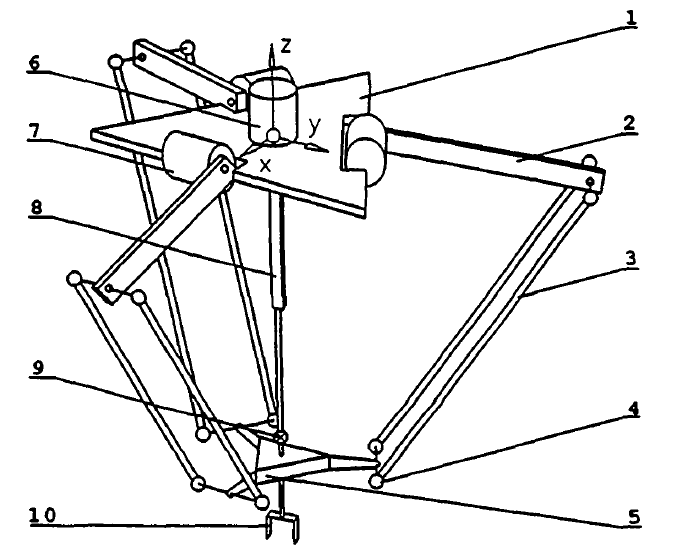
\includegraphics[width=0.5\textwidth]{Main/Chapter3/Images3/3-3/esquema-principal-robot-delta.png}}
              \subfloat[Representación de paralelogramos del robot delta]{
               \label{f:Cap3-3_ayuda_dimensiones}
                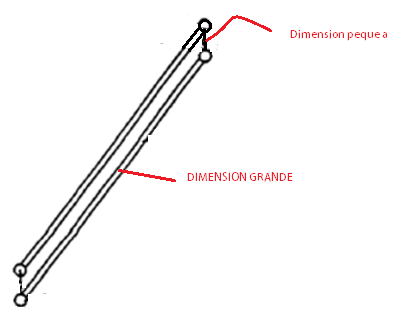
\includegraphics[width=0.5\textwidth]{Main/Chapter3/Images3/3-3/ayuda-dimensiones.png}}
         \caption{Descripción visual de un robot delta \cite{Clavel:31403}}
         %\label{f:animales}
    \end{figure}

    La orientación de la góndola está asegurada constantemente por los 3 paralelogramos (figura \eqref{f:Cap3-3_ayuda_dimensiones}), que comprenden cada uno 2 dimensiones pequeñas y 2 dimensiones grandes formadas por las barras paralelas. Cada lado pequeño integrado al extremo de un brazo permanece constantemente paralelo al eje de rotación del brazo en cuestión. Los 3 pares de barras paralelas aseguran que las 3 pequeñas dimensiones integradas a la góndola permanezcan paralelas a las pequeñas dimensiones integradas a los extremos de los brazos, por tanto, paralelas a los ejes de rotación de los brazos que, por construcción, se ubican en el mismo plano. Las juntas en los extremos de las barras paralelas son del tipo de junta esférica, por lo que cada barra puede girar alrededor de su eje longitudinal; esta rotación no altera el comportamiento de esta estructura articulada que forma el paralelogramo del espacio. Una conexión por resortes y estribos entre las 2 barras paralelas simplifica la construcción de las rótulas.
    
    \newpage

\section{Software Robot Operating System (ROS)}
    
        En esta sección se proporciona una descripción general de Robot Operating System (sus siglas ROS) y sus principales lineamientos. ROS es un marco para desarrollar software de robótica. El software está estructurado bajo un paradigma modular, pequeños paquetes que se comunican entre si mediante rápidos mensajes. Este paradigma se fomenta la reutilización de código y la colaboración global por sobre los entornos particulares.
    
    \begin{figure}[htb]
        \centering
        
\includegraphics[width=0.5\linewidth]{Main/Chapter3/Images3/3-4/logo-ros.png}
        \caption{Logo de ROS \cite{ros2222}}
        \label{f:Cap3-4_logo_ros}
    \end{figure}
    
    \subsection{Historia}
    
        ROS es un gran proyecto que tiene muchos antepasados y contribuyentes. Mucha gente en la comunidad de investigación robótica sintió la necesidad de un marco de colaboración abierto. Varios proyectos en la Universidad de Stanford (figura \eqref{f:Cap3-4_entidades_inicio_ros_32}) a mediados de la década de 2000 involucraban inteligencia artificial incorporada e integradora, como el Stanford AI Robot (STAIR) y el programa Personal Robots (PR), que crearon prototipos internos de los tipos de sistemas de software dinámicos y flexibles como lo es ROS. Se basó en Switchyard, que era parte de un proyecto de STAIR y fue escrito por Morgan Quigley en Stanford. En 2007, Willow Garage, Inc., una incubadora de robótica cercana, proporcionó importantes recursos para extender estos conceptos mucho más y crear implementaciones bien probadas. Desde el 2013 hasta el presente, ROS es mantenido permanentemente por Open Source Robotics Foundation (OSRF, figura \eqref{f:Cap3-4_entidades_inicio_ros_334}) de Google y desde el 2017 cambio su nombre a Open Robotics.
        
        \begin{figure}[htbp]
            \centering
            
\includegraphics[width=0.7\linewidth]{Main/Chapter3/Images3/3-4/entidade-asociadas-al-inicio-de-ros-3.png}
            \caption{OSRF \cite{osrf}} 
            \label{f:Cap3-4_entidades_inicio_ros_334}
        \end{figure}        
        
        \newpage
        
        La mayoría de las compañías y laboratorios de investigación en robótica están ahora portando su software a ROS. Esta tendencia también es visible en robots industriales, donde compañías están paulatinamente migrando de aplicaciones propietarias a ROS. El movimiento llamado ROS Industrial se ha incrementado en estos últimos años y su objetivo básicamente consiste en extender las capacidades avanzadas de ROS a la automatización y la robótica industrial. Este proyecto comenzó como un intento de colaboración de Yaskawa Motoman Robotics, Southwest Research Institute (SwRI) y Willow Garage (figura \eqref{f:Cap3-4_entidades_inicio_ros_33364}). En enero de 2012, Shaun Edwards de SwRI fundó un software repositorio, alojado en Github, donde la comunidad robótica puede encontrar interfaces para manipuladores industriales, pinzas, sensores y redes de dispositivos.
        
        \begin{figure}[htbp]
            \centering
            
\includegraphics[width=0.65\linewidth]{Main/Chapter3/Images3/3-4/entidade-asociadas-al-inicio-de-ros-2.png}
            \caption{Fundadores y contribuidores de ROS} 
            \label{f:Cap3-4_entidades_inicio_ros_33364}
        \end{figure}    
        
        Finalizando con la breve historia de ROS, se puede decir que se utiliza en estos momentos en todo el mundo en instituciones académicas, industriales y de investigación. Los desarrolladores han contribuido con miles de paquetes, incluyendo soluciones de algunos de los principales expertos del mundo en áreas específicas. Las nuevas empresas de robots ofrecen interfaces ROS con sus productos y las empresas de robots industriales ya establecidas también están introduciendo ROS. Con la adopción generalizada de ROS como el enfoque estándar de factor para la programación de robots, existe una nueva esperanza de acelerar las capacidades de los robots exponencialmente.
        
        \begin{figure}[htbp]
            \centering
            
\includegraphics[width=0.6\linewidth]{Main/Chapter3/Images3/Stanford-University-logo1.jpg}
            \caption{Logo Stanford University \cite{stanford}} 
            \label{f:Cap3-4_entidades_inicio_ros_32}
        \end{figure}

    \newpage

    \subsection{Problema Principal}
    
    ROS se creó con la intención de permitirle a los investigadores desarrollar rápidamente nuevos sistemas robóticos sin necesidad de reinventar todo nuevamente, mediante el uso de herramientas e interfaces estándar. Para hacer más eficientes los procesos de investigación y de desarrollo de software de robots, se detectaron los siguientes 3 problemas a solucionar:
    
    \begin{itemize}
        \item {Programación secuencial es inadecuada para el mundo asincrónico robótico (figura \eqref{f:Cap3-4_entidades_ini_ros_1})}
        \item {Los sistemas robóticos deben gestionar una complejidad significativa}
        \item {La abstracción de los detalles de un hardware específico de un robot es difícil.}
    \end{itemize}

        \begin{figure}[htbp]
            \centering
            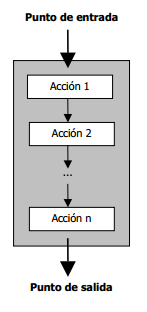
\includegraphics[width=0.25\linewidth]{Main/Chapter3/Images3/agrupar_problem_111.png}
            \caption{Programación Secuencial}
            \label{f:Cap3-4_entidades_ini_ros_1}
        \end{figure}
        
    La solución para el problema de programación secuencias se basó en “callback”, que son una función que se ejecuta siempre que hay datos disponibles para su procesamiento. Son asincrónico, ya que la devolución de llamada puede ocurrir en cualquier momento. Con respecto a el problema de softwares multifuncionales complejos y atracción de detalles de hardware específicos, se separaron los procesos en “nodos” que se comunican a través de una interfaz de mensajería. Por ejemplo, se separaron los procesos de las cámaras, edometría, escáner láser y creación de mapas y estos interactúan a través de una interfaz que comunica estos procesos por medio de “temas”. Estos últimos conceptos se explican en detalle en secciones posteriores.

    \newpage


    \subsection{Que es ROS}
       ROS es una abreviatura de  Robot Operating System y es una plataforma de desarrollo de aplicaciones en robótica que provee estilos de programación (en particular, que se basa en nodos distribuidos y acoplados libremente); definiciones de interfaz y paradigmas para las comunicaciones entre nodos ; definiciones de interfaz para la incorporación de bibliotecas y paquetes; una colección de herramientas para visualización, depuración, registro de datos y diagnóstico del sistema; un repositorio de código fuente compartido; y puentes a múltiples bibliotecas útiles e independientes de código abierto.
       
       El objetivo principal de ROS es apoyar la reutilización de código en la investigación y el desarrollo de robótica. ROS es un marco distribuido de procesos (también conocido como nodos) que permite que los ejecutables se diseñen individualmente y se acoplen libremente en tiempo de ejecución. Estos procesos se pueden agrupar en paquetes, que se pueden compartir y distribuir fácilmente. ROS también es compatible con un sistema federado de repositorios de código que también permite la distribución de la colaboración. Este diseño, desde el nivel del sistema de archivos hasta el nivel de la comunidad, permite decisiones independientes sobre el desarrollo y la implementación, pero todos pueden combinarse con las herramientas de infraestructura ROS.
       
       ROS no es un sistema operativo convencional como Windows, Linux y Android en el sentido tradicional de gestión y programación de procesos; más bien, es un meta-sistema operativo que se ejecuta en el sistema operativo. Las diferencias entre un OS y ROS se muestran el la figura \eqref{f:Cap3-4_diferencias_ros_so}. ROS es un middleware, que proporciona los servicios que se espera de un sistema operativo, incluida la abstracción de hardware, control de dispositivos de bajo nivel, implementación de funciones de uso común, transmisión de mensajes entre procesos y administración de paquetes. También proporciona herramientas y bibliotecas para obtener, compilar, escribir y ejecutar código en varios equipos.
       
        \begin{figure}[htb]
            \centering
            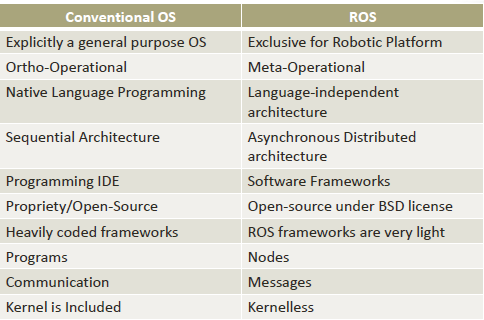
\includegraphics[width=0.65\linewidth]{Main/Chapter3/Images3/3-4/diferencia-ROS-SO.png}
            \caption{Diferencias entre un sistema operativo convencional y ROS}
            \label{f:Cap3-4_diferencias_ros_so}
        \end{figure}
        
        \newpage
        
        Las principales características de ROS se pueden resumir de la siguiente manera:
        
        \begin{itemize}
            \item \textbf{Plumbing:} ROS proporciona una infraestructura de mensajería de publicación y suscripción diseñada para respaldar la construcción rápida y sencilla de sistemas informáticos distribuidos.
            \item \textbf{Herramientas} ROS proporciona un amplio conjunto de herramientas para configurar, iniciar, introspectar, depurar, visualizar, registrar, probar y detener sistemas informáticos distribuidos.
            \item \textbf{Capacidades} ROS proporciona una amplia colección de bibliotecas que implementan funcionalidades robóticas útiles, con un enfoque en la movilidad, la manipulación y la percepción.
            \item \textbf{Ecosistema:} ROS es apoyado y mejorado por una gran comunidad, con un fuerte enfoque en la integración y documentación. \url{https://www.ros.org/} es una ventanilla única que busca y aprende sobre los miles de paquetes ROS que están disponibles a través de desarrolladores de todo el mundo.
        \end{itemize}

        La figura \eqref{f:Cap3-4_compatibilidad_ros} muestra que la comunicación de datos ROS es compatible no solo con un sistema operativo, sino también con múltiples sistemas operativos, hardware y programas, lo que lo hace muy adecuado para el desarrollo de robots donde se combinan varios hardware. 
        
        \begin{figure}[htb]
            \centering
            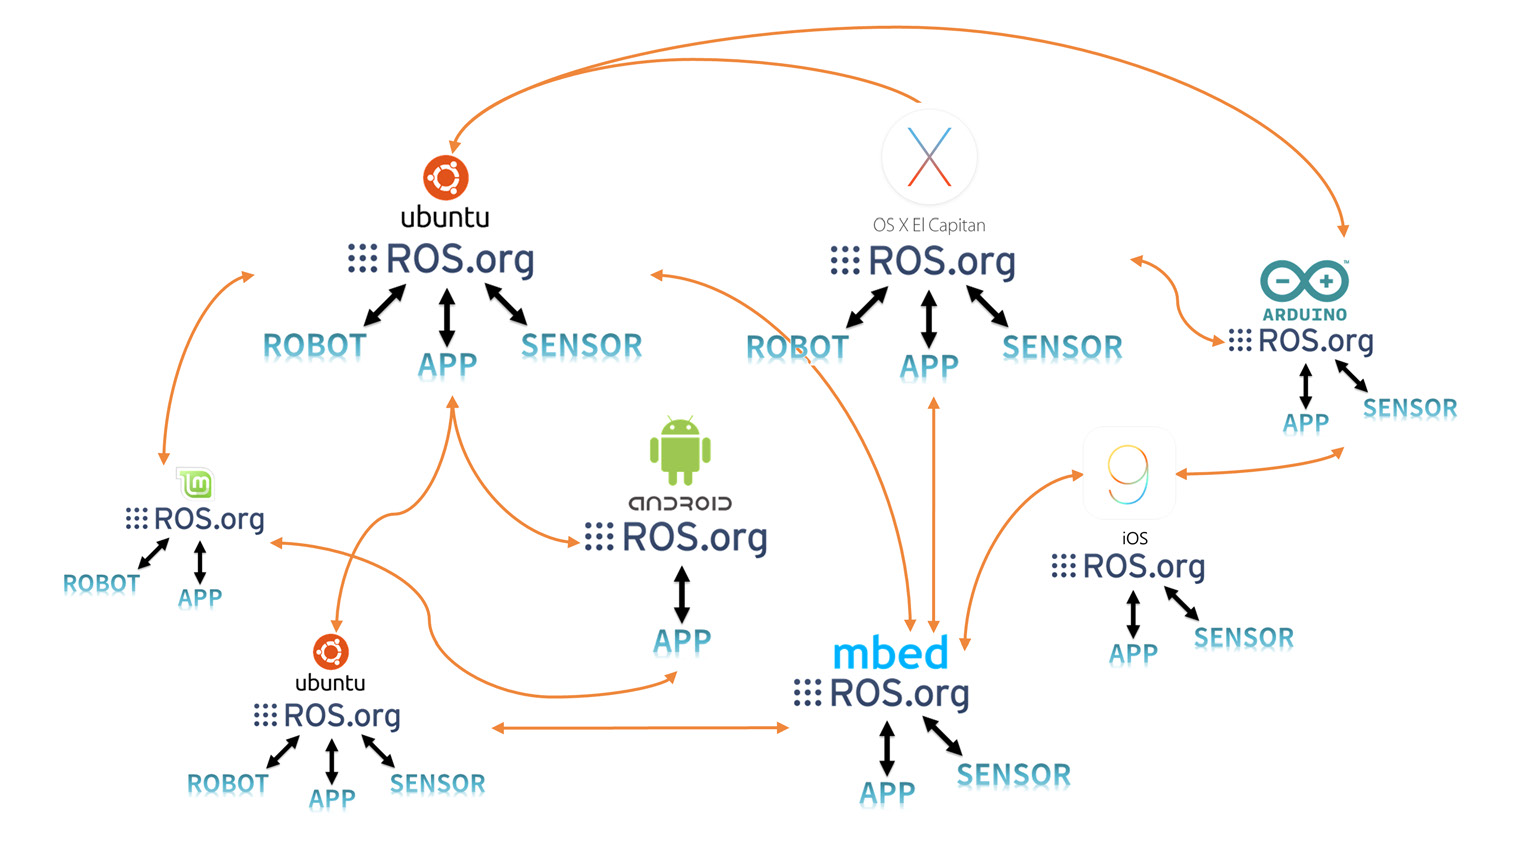
\includegraphics[width=1.0\linewidth]{Main/Chapter3/Images3/3-4/compatibilidad-ros.png}
            \caption{Compatibilidad de ROS y otras plataformas \cite{ROS_BOOK_1}}
            \label{f:Cap3-4_compatibilidad_ros}
        \end{figure}
        
    \newpage

        
    \subsection{Objetivos de ROS}
    
        Todos los marcos de software imponen sus filosofías de desarrollo a sus colaboradores directa o indirectamente, a través de sus modismos y prácticas comunes. En términos generales, ROS sigue la filosofía de desarrollo de software de Unix en varios aspectos clave. Esto tiende a hacer que ROS se sienta ``natural'' para los desarrolladores que provienen de Unix, pero algo ``críptico'' al principio para aquellos que han utilizado principalmente entornos de desarrollo gráfico en Windows o Mac OS X. Los siguientes párrafos describen varios aspectos filosóficos de ROS.
        
        \subsubsection{Peer to peer (Nodos)}
        
            Los sistemas ROS consisten en numerosos programas pequeños de computadora que se conectan entre sí e intercambian mensajes continuamente. Estos mensajes viajan directamente de un programa a otro; no hay un servicio de enrutamiento central. Aunque esto hace que la ``plumbing'' subyacente sea más compleja, el resultado es un sistema que escala mejor a medida que aumenta la cantidad de datos. La mentalidad Peer to peer se representa en la figura \eqref{f:Cap3-5_arquitectura_ros}.
            
            \begin{figure}[htb]
                \centering
                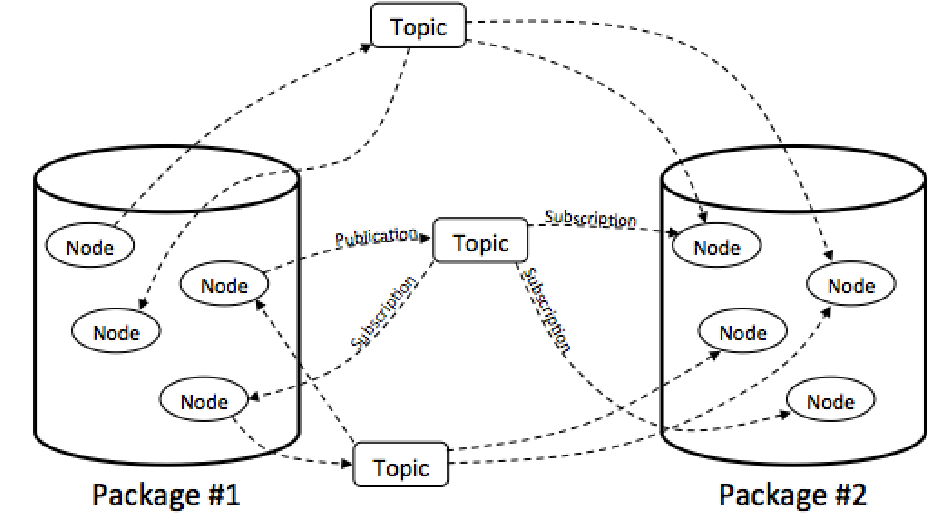
\includegraphics[width=0.8\linewidth]{Main/Chapter3/Images3/arquitectura_por_nodos_1.png}
                \caption{Modelo de comunicación ROS: nodos publican y se suscriben a temas \cite{naval_delta}}
                \label{f:Cap3-5_arquitectura_ros}
            \end{figure}
            
        \subsubsection{Orientación hacia las herramientas}
        
            Como lo demuestra la arquitectura duradera de Unix, se pueden crear sistemas de software complejos a partir de muchos programas pequeños y genéricos. A diferencia de muchos otros marcos de software de robótica, ROS no tiene un entorno de ejecución y desarrollo integrado canónico. Tareas como navegar por el árbol del código fuente, visualizar las interconexiones del sistema, trazar gráficamente los flujos de datos, generar documentación, registrar datos, etc, son todas realizadas por programas separados. Esto fomenta la creación de implementaciones nuevas y mejoradas, ya que (idealmente) se pueden intercambiar por implementaciones más adecuadas para un dominio de tarea en particular. Las versiones recientes de ROS permiten que muchas de estas herramientas se compongan en procesos únicos para mayor eficiencia o para crear interfaces coherentes para operadores o depuración, pero el principio sigue siendo el mismo: las herramientas individuales en sí mismas son relativamente pequeñas y genéricas.
            
        \subsubsection{Multilenguaje}
        
            Muchas tareas de software son más fáciles de realizar en lenguajes de secuencias de comandos de ''alta productividad'' como Python o Ruby. Sin embargo, hay ocasiones en las que los requisitos de rendimiento exigen el uso de lenguajes más rápidos, como C ++. También hay varias razones por las que algunos programadores prefieren lenguajes como Lisp o MATLAB. Se han librado guerras interminables de correo electrónico, se están librando actualmente y, sin duda, se seguirá librando sobre qué idioma es el más adecuado para una tarea en particular. Reconociendo que todas estas opiniones tienen mérito, que los lenguajes tienen diferentes utilidades en diferentes contextos, y que la experiencia única de cada programador es muy importante al elegir un idioma, ROS eligió un enfoque multilingüe. Los módulos de software ROS se pueden escribir en cualquier idioma para el que se haya escrito una biblioteca cliente. En el momento de escribir este artículo, existen bibliotecas cliente para C ++, Python, LISP, Java, JavaScript, MATLAB, Ruby, Haskell, R, Julia y otros. Las bibliotecas de cliente ROS se comunican entre sí siguiendo una convención que describe cómo los mensajes se ``aplanan'' o ``serializan'' antes de transmitirse a través de la red. La figura \eqref{f:Cap3-5_multilenguaje_ros} representa un ejemplo de multilenguaje en ROS. En ella se muestra el nodo ''Laser Scanner'' escrito en lenguaje Python con el objetivo de obtener datos de un entorno físico por medio de un escáner de láser y el nodo ''Map Building'' escrito en lenguaje C++ es el encargado de transformar los datos obtenidos por del nodo anterior para poder visualizarlos a la computadora.     
            
            \begin{figure}[htb]
                \centering
                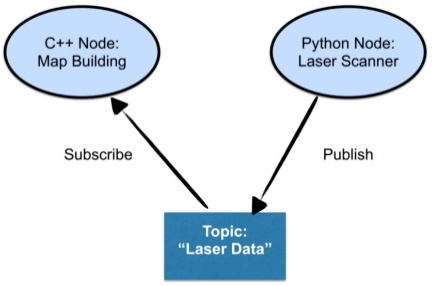
\includegraphics[width=0.5\linewidth]{Main/Chapter3/Images3/multilenguaje_1.png}
                \caption{Ejemplo de multilenguaje de ROS}
                \label{f:Cap3-5_multilenguaje_ros}
            \end{figure}

\newpage
            
        \subsubsection{Pequeño}
        
            Las convenciones ROS alientan a los contribuyentes a crear bibliotecas independientes y luego empaquetar esas bibliotecas para que puedan enviar y recibir mensajes hacia y desde otros módulos ROS. Esta capa adicional está destinada a permitir la reutilización de software fuera de ROS para otras aplicaciones, y simplifica en gran medida la creación de pruebas automatizadas utilizando herramientas de integración continua estándar.
            
        \subsubsection{Libre y Open Source}
        
            El núcleo de ROS se publica bajo la licencia BSD permisiva, que permite el uso comercial y no comercial. ROS pasa datos entre módulos mediante comunicación entre procesos (IPC), lo que significa que los sistemas construidos con ROS pueden tener licencias detalladas de sus diversos componentes. Los sistemas comerciales, por ejemplo, a menudo tienen varios módulos de fuente cerrada que se comunican con una gran cantidad de módulos de fuente abierta. Los proyectos académicos y de pasatiempos suelen ser de código abierto. El desarrollo de productos comerciales a menudo se realiza completamente detrás de un firewall. Todos estos casos de uso, y más, son comunes y perfectamente válidos bajo la licencia ROS.
            
            \begin{figure}[htb]
                \centering
                
\includegraphics[width=0.3\linewidth]{Main/Chapter3/Images3/3-5/licnecia-bsd-ros.png}
                \caption{Licencia de ROS}
                \label{f:Cap3-5_multilenguaje_ros}
            \end{figure}
            

\newpage

    \subsection{Estadisticas}
    
    \subsubsection{Science Robotics}
        La revista Science Robotics publicó un articulo el año 2017 llamado “Powering the world’s robots 10 years of ROS” \cite{Zhangeaar1868} que habla sobre la iniciativa ROS-I (Ros Industrial) lanzada el año 2012. Debido a las arquitecturas de software limitadas de los robots industriales actuales, es demasiado caro aplicar capacidades robóticas avanzadas para mejorar la productividad industrial. ROS-I proporciona interfaces para robots industriales comunes y dispositivos sensoriales junto con bibliotecas de software específicas para la automatización de la fabricación. ROS-I ha apoyado un número creciente de hardware industrial, como los robots producidos por ABB, Fanuc y Yaskawa. Además, el Consorcio ROS-I existe para desarrollar la comunidad ROS-I proporcionando apoyo técnico, organizando cursos de capacitación y talleres, estableciendo la hoja de ruta para ROS-I. El Consorcio ROS-I tiene más de 50 miembros en todo el mundo, incluidos institutos de investigación y agencias gubernamentales, integradores de sistemas y usuarios finales, y fabricantes de equipos originales. Además, la próxima versión de ROS 2.0 debería abordar una de las principales limitaciones que ha ralentizado la adopción de ROS en la industria: que es una implementación de middleware interna. ROS 2.0 ahora se basa en el servicio de distribución de datos para la comunicación entre procesos, lo que brinda una confiabilidad mucho mejor con protocolos de calidad de servicio y seguridad con cifrado.

        La figura \eqref{f:Cap3-5_estadisticas_1} muestra algunas estadísticas clave de ROS, las cuales son:

            \begin{figure}[htb]
                \centering
                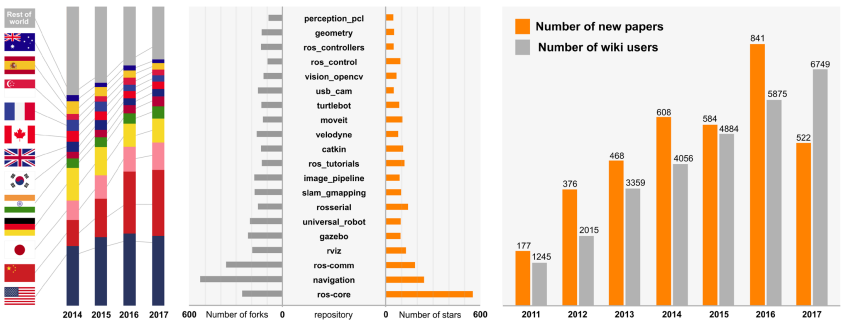
\includegraphics[width=1.0\linewidth]{Main/Chapter3/Images3/science_robot_esta_1.png}
                \caption{Estadísticas mundiales de ROS \cite{Zhangeaar1868}}
                \label{f:Cap3-5_estadisticas_1}
            \end{figure}        

        \begin{itemize}
            \item {\textbf{Los países visitantes de la wiki de ROS:} en los últimos 4 años muestra un cambio creciente de investigadores de países del lejano oriente (información recolectada del informe métrico anual de ROS). }
            \item {\textbf{Los 20 principales repositorios ROS:}  según la cantidad de bifurcaciones y estrellas (de Github, 10 de octubre de 2017).}
            \item {\textbf{Artículos recientemente publicados:} en los últimos 10 años que han citado el artículo ''ROS original'' (de la búsqueda de Google Scholar, palabras clave “Sistema operativo de robot ROS”) y el número de usuarios de wiki registrados.}
        \end{itemize}
        

        La figura \eqref{f:Cap3-5_estadisticas_2} muestra los diez años de desarrollos de ROS que respaldan la investigación y el desarrollo, incluida la robótica móvil, industrial, quirúrgica y espacial, así como los automóviles autónomos. Se han lanzado 11 distribuciones de ROS en los últimos 10 años, y el gráfico de barras muestra el número de descargas binarias de ROS en cada año. El Consorcio ROS-I se lanzó en 2013 con el objetivo de transformar las capacidades de ROS en tiempo real para robots industriales. ROS 2.0 esta actualmente en desarrollo intenso, y se acaba de lanzar una versión beta.

            \begin{figure}[htb]
                \centering
                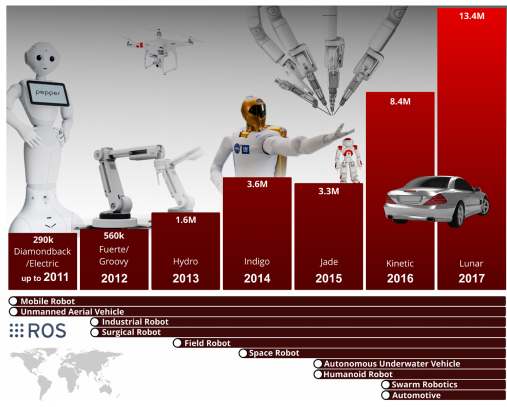
\includegraphics[width=1.0\linewidth]{Main/Chapter3/Images3/science_robot_esta_2.png}
                \caption{Desarrollo de ROS en los últimos 10 años \cite{Zhangeaar1868}}
                \label{f:Cap3-5_estadisticas_2}
            \end{figure}  


         \newpage
    
        \subsubsection{Metricas de la comunidad ROS}
    
    Ros Metrics miden aspectos de la comunidad ROS para comprender y rastrear el impacto de su trabajo e identificar áreas de mejora. Se inspiran en las métricas del Proyecto MeeGo .
    
        \begin{figure}[htb]
            \centering
            
\includegraphics[width=0.4\linewidth]{Main/Chapter3/Images3/cap3_estadisticas_3.png}
            \caption{Logo de ROS Metrics \cite{rosmetrics}}
            \label{f:Cap3-5_estadisticas_3}
        \end{figure}  
        
        Las figuras \eqref{f:Cap3-5_estadisticas_4} y \eqref{f:Cap3-5_estadisticas_5} presentan estadísticas recolectadas de la pagina oficial de ROS Metrics hasta el año 2021. Según la figura \eqref{f:Cap3-5_estadisticas_4}, los países que más han visitado ROS son China, EEUU, Japón y Alemania. 
        
        \begin{figure}[htb]
            \centering
            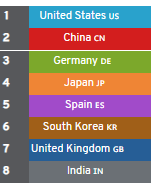
\includegraphics[width=0.27\linewidth]{Main/Chapter3/Images3/cap3_estadisticas_7.png}
            \caption{Top de países que utilizan ROS en base a la descarga de paquetes registrados hasta el 28 de marzo del año 2021 \cite{rosmetrics}.}
            \label{f:Cap3-5_estadisticas_4}
        \end{figure}  
        

        \begin{figure}[htb]
            \centering
            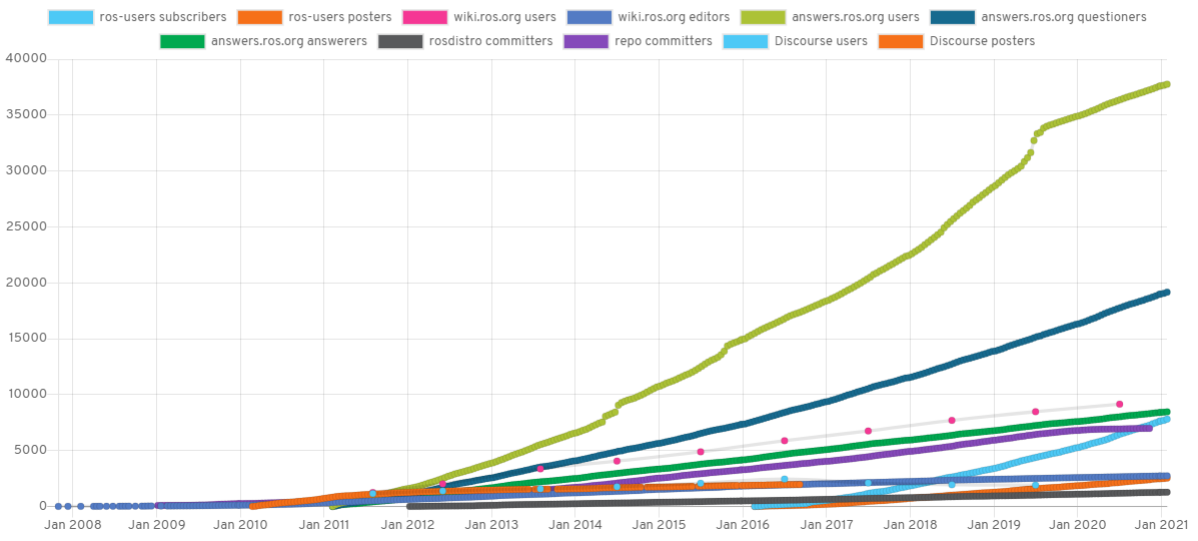
\includegraphics[width=1.0\linewidth]{Main/Chapter3/Images3/cap3_estadisticas_4.png}
            \caption{Colección de diferentes métricas para medir la cantidad de usuarios de la comunidad ROS \cite{rosmetrics}}
            \label{f:Cap3-5_estadisticas_5}
        \end{figure}  
        
        \newpage

        \subsubsection{Repositorio GitHub}
            Para comprender GitHub, primero se debe comprender Git. Git es un sistema de control de versiones de código abierto que fue iniciado por Linus Torvalds, la misma persona que creó Linux. Sirve para cuando los desarrolladores crean algo (una aplicación, por ejemplo), realizan cambios constantes en el código, lanzando nuevas versiones hasta y después del primer lanzamiento oficial. Los sistemas de control de versiones mantienen estas revisiones en orden, almacenando las modificaciones en un repositorio central. Esto permite a los desarrolladores colaborar fácilmente, ya que pueden descargar una nueva versión del software, realizar cambios y cargar la revisión más reciente. Todos los desarrolladores pueden ver estos nuevos cambios, descargarlos y contribuir. Del mismo modo, las personas que no tienen nada que ver con el desarrollo de un proyecto aún pueden descargar los archivos y usarlos. Git es una herramienta de línea de comandos, pero el centro alrededor del cual giran todas las cosas relacionadas con Git es el centro Github, donde los desarrolladores almacenan sus proyectos y se conectan con personas de ideas afines.
    
            \begin{figure}[htb]
            \centering
            
\includegraphics[width=0.21\linewidth]{Main/Chapter3/Images3/repo_git_1.png}
            \caption{Logo GitHub, Inc.}
            \label{f:Cap3-5_estadisticas_8}
            \end{figure} 
        
            Dirk Thomas trabajó en ROS durante casi 9 años y envio 15 distribuciones de ROS. Uno de los paquetes que subió al repositorio de GitHub registra el total de autores, commits y repositorios en Github con relación a ROS hasta octubre del 2020 (figura \ref{f:Cap3-5_estadisticas_9}).
        
            \begin{figure}[htb]
            \centering
            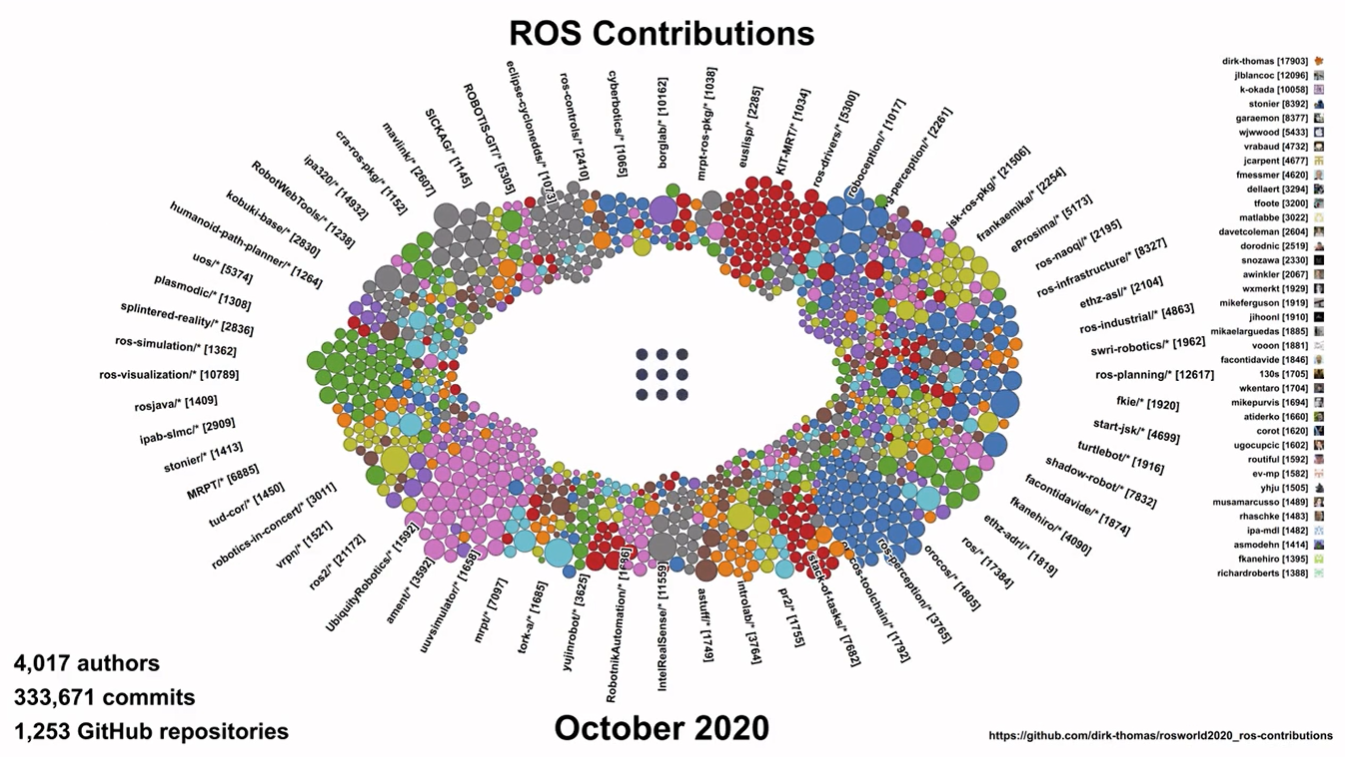
\includegraphics[width=0.99\linewidth]{Main/Chapter3/Images3/repo_git_2.png}
            \caption{Visualización de las contribuciones de ROS en GitHub \cite{gitreposito}}
            \label{f:Cap3-5_estadisticas_9}
            \end{figure} 
    
        \newpage

    \subsection{Versiones}
            En 2007, Willow Garage logró la investigación del marco de software de robot que comenzó en el laboratorio de inteligencia artificial de la Universidad de Stanford y continuó el desarrollo bajo el nombre de Robot Operating System. Con la sexta versión de lanzamiento oficial "ROS Groovy Galápagos", Willow Garage intentó penetrar en el mercado de robots de servicios comerciales en 2013, pero terminó dividiéndose en varias empresas emergentes y finalmente se entregó a la Open Source Robotics Foundation. Desde entonces, se lanzaron 4 versiones más y, a partir de mayo de 2017, OSRF cambió su nombre a Open Robotics y ha estado desarrollando, operando y administrando ROS. Más recientemente, la undécima versión de ROS, ROS Lunar Loggerhead, fue lanzada el 23 de mayo de 2017. ROS etiqueta la primera letra de cada nombre de lanzamiento en orden alfabético y usa una tortuga como su símbolo (ver figura \eqref{f:Cap3-5_estadisticas_10}).
            
            \begin{figure}[htb]
            \centering
            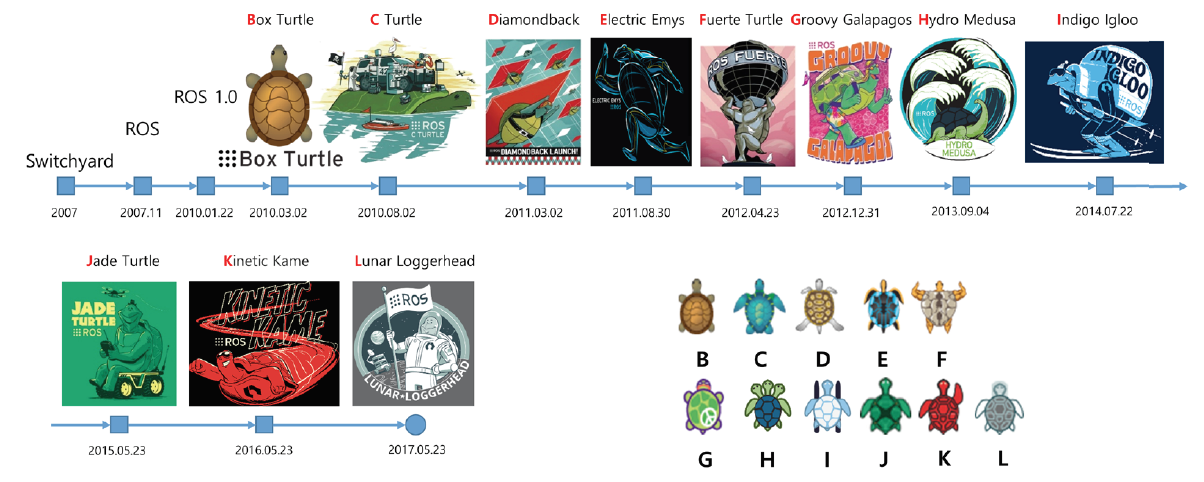
\includegraphics[width=0.94\linewidth]{Main/Chapter3/Images3/ver_ros_1.png}
            \caption{Linea temporal e iconos de tortuga para cada versión de ROS \cite{ROS_BOOK_1}}
            \label{f:Cap3-5_estadisticas_10}
            \end{figure} 
    
            \begin{figure}[htb]
            \centering
            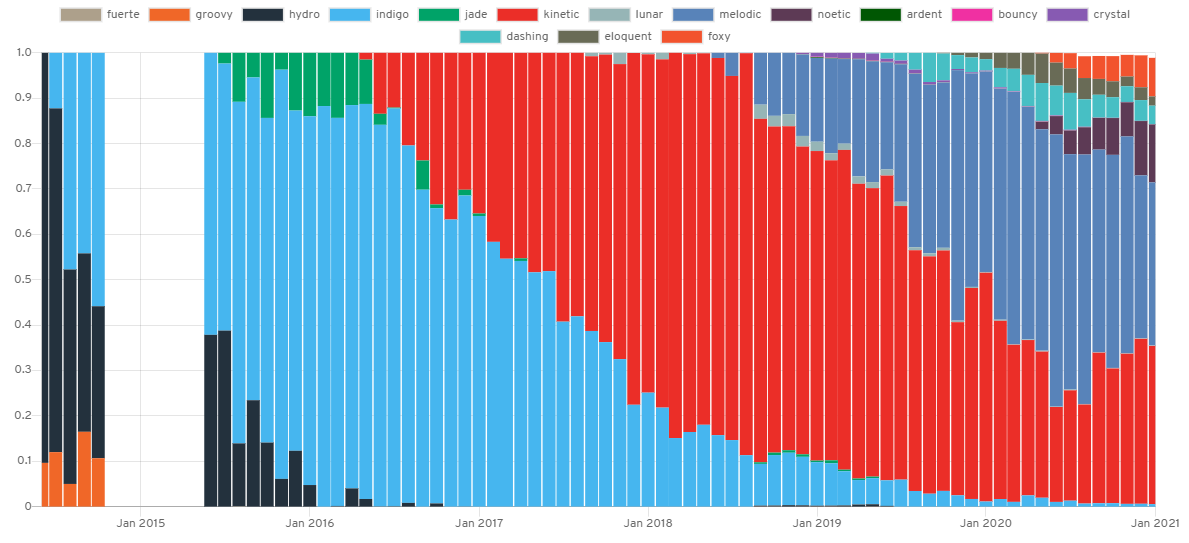
\includegraphics[width=0.94\linewidth]{Main/Chapter3/Images3/ver_ros_2.png}
            \caption{Uso relativo de cada versión de ROS basado en descargas desde packages.ros.org \cite{rosmetrics}.}            \label{f:Cap3-5_estadisticas_11}
            \end{figure} 
    
    \newpage
    
    \subsection{Conceptos principales}
            
            Existen tres niveles de conceptos en ROS. El primer nivel llamado ''nivel de sistema de archivos'' se refiere a la manera en que diferentes archivos están organizados en la computadora, herramientas ROS para administrar código fuente, instrucciones de compilación y definiciones de mensajes. El segundo nivel llamado ''nivel de gráfico computacional'' son los componentes de la red peer to peer de nodos ROS, es decir, los procesos. Por último, el tercer nivel llamado ''nivel comunitario'' se relaciona con la forma en que los usuarios comparten software para permitir que todos lo utilicen.
            
            \begin{figure}[htb]
                \centering
                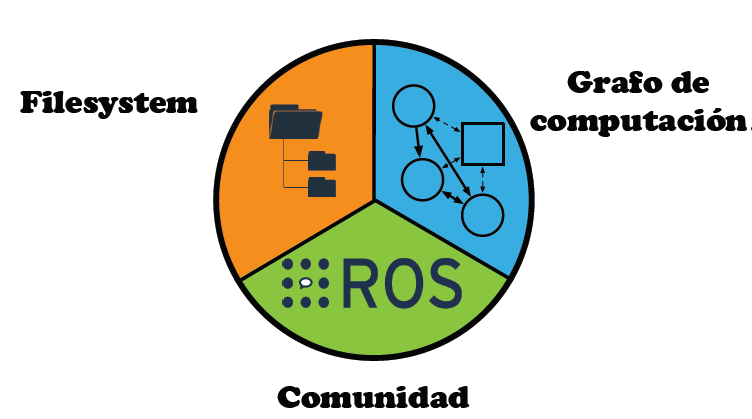
\includegraphics[width=1\linewidth]{Main/Chapter3/Images3/nivel_s_a_1.png}
                \caption{Niveles de conceptos de ROS}
                \label{f:Cap3_conceptos_1}
            \end{figure} 
            

                
                
               \newpage
               
            \subsubsection{Nivel de sistemas de archivos}

                Similar a un sistema operativo, los archivos de ROS también se organizan en el disco duro de una manera particular. En este nivel, se puede ver cómo se organizan estos archivos en el disco. La figura \eqref{f:Cap3_conceptos_2} muestra cómo se organizan los archivos y carpetas:
                
                
            \begin{figure}[htb]
                \centering
                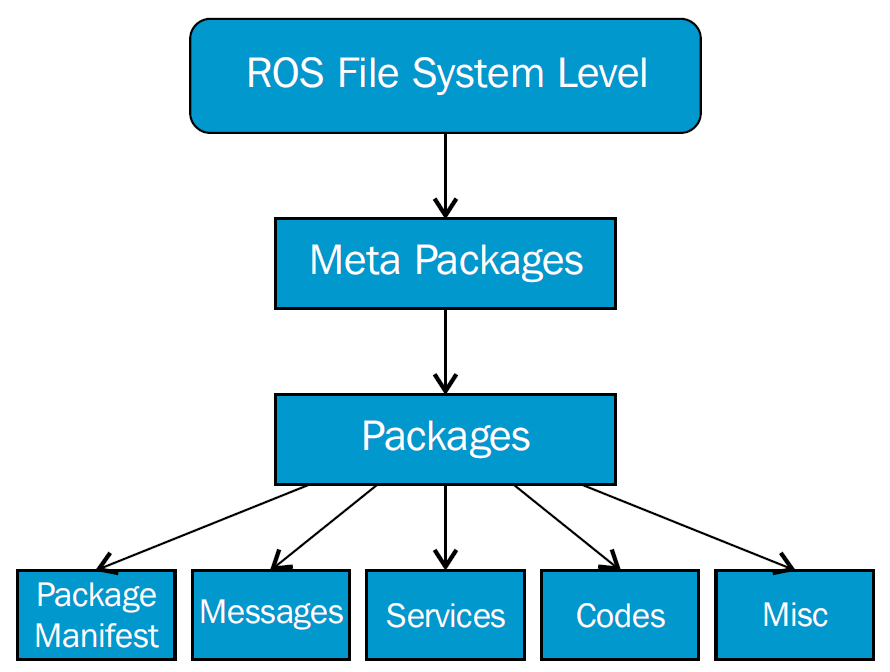
\includegraphics[width=0.55\linewidth]{Main/Chapter3/Images3/n_s_a_2.png}
                \caption{Nivel de sistema de archivos ROS \cite{lentin_2015}}
                \label{f:Cap3_conceptos_2}
            \end{figure} 
                
                

            A continuación se presenta la descripción de cada bloque en el sistema de archivos:
            \begin{itemize}
                \item {\textbf{Meta packages:} Es un único paquete lógico compuesto por muchos paquetes en su interior. Además, los meta paquetes contienen un archivo package.xml que describe la carpeta y sus dependencias.}
                \item {\textbf{Packages:} Son las unidades más bajas y la principal para organizar el software en ROS. Un paquete puede contener procesos en tiempo de ejecución ROS (nodos), un biblioteca dependiente de ROS, conjuntos de datos, archivos de configuración o achivos de lanzamiento. Cada directorio de paquete debe incluir un archivo CMakeList.txt y package.xml que describa el contenido del paquete y cómo catkin debe interactuar con él.}
                \item {\textbf{Stacks:} Son grupos de paquetes que se juntan para realizar funciones de alto nivel.}
                \item {\textbf{Manifests:} Los manifiestos proporcionan metadatos sobre un paquete. Pueden pertenecer a un packages o una Stacks y describen información general sobre un paquete o Stacks específico, como una breve descripción de lo que hace, el nombre del autor, su tipo de licencia y las dependencias.con otros paquetes.}
                \item {\textbf{Message (msg) types:} Las descripciones de los mensajes definen los datos estructuras para mensajes enviados en ROS.}
                \item {\textbf{Service (srv) types:} Las descripciones de servicio definen la solicitud y estructuras de datos de respuesta para servicios en ROS.}
            \end{itemize}
            
               \newpage
               
            ROS está basado en CMake y puede ser utilizado por muchos sistemas operativos como Linux o Windows. CMake es un generador de herramientas de creación, es una herramienta de nivel superior que simplifica el proceso de compilación y construcción. Puede gestionar grandes proyectos y tiene una buena escalabilidad. Para una plataforma a gran escala como ROS, ha extendido CMake a un sistema de compilación llamado Catkin. Catkin es el sistema de compilación de ROS que genera programas ejecutables, bibliotecas e interfaces y proporciona el concepto de espacio de trabajo en la construcción de cada proyecto.
            
            La estructura del espacio de trabajo catkin, incluye las carpetas /src, /build, /devel. Las tres rutas también pueden incluir otras en algunas opciones de compilación pero estas tres carpetas son las predeterminadas para el sistema de compilación catkin. Sus roles específicos son los siguientes:

            \begin{itemize}
                \item {\textbf{Espacio fuente (/src):} Contiene el código fuente donde el usuario puede extraer, verificar o clonar el código fuente de los paquetes que quiere construir.}
                \item {\textbf{Espacio de construcción (/build):} Este es el espacio donde CMake apela para construir los paquetes en el espacio de trabajo de catkin. CMake y Catkin mantienen su información de caché y otros intermedios archivos.}
                \item {\textbf{Espacio de desarrollo (/devel):} Se encuentran archivos de objetos generados (incluidos archivos de encabezado, bibliotecas de vínculos dinámicos, bibliotecas de vínculos estáticos, archivos ejecutables, etc.) y variables de entorno.}
            \end{itemize}


            Durante el proceso de compilación, el flujo de trabajo de un catkin workspace es el que se muestra con flechas azules en la figura \eqref{f:Cap3_conceptos_3}. Los dos últimos procesos son generados y administrados automáticamente por el sistema catkin. El uso principal para los usuarios de ROS es la carpeta src\/, donde los paquetes creados o copiados se almacenan en dicha carpeta. En el momento de la compilación, el sistema de compilación de catkin busca y compila todos los paquetes de código fuente de forma de la ruta /src\/.

            \begin{figure}[htb]
                \centering
                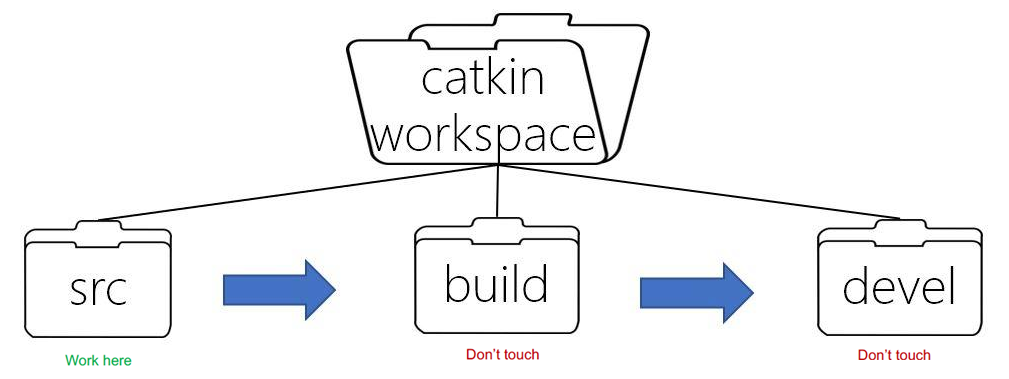
\includegraphics[width=0.8\linewidth]{Main/Chapter3/Images3/n_s_a_3.png}
                \caption{Espacio de trabajo catkin\_make \cite{cmake_blogcsdn}}
                \label{f:Cap3_conceptos_3}
            \end{figure} 
            
               \newpage


            Cuando se crea un paquete, normalmente es común encontrar las carpetas que se muestran en la figura \eqref{f:Cap3_conceptos_4}:
            
            \begin{figure}[htb]
                \centering
                \includegraphics[width=1.0\linewidth]{Main/Chapter3/Images3/n_s_a_4.png}
                \caption{Estructura y características de catkin\_make \cite{cmake_blogcsdn}}
                \label{f:Cap3_conceptos_4}
            \end{figure} 

            \begin{itemize}
                \item {\textbf{/include/:} Esta carpeta contiene los encabezados (*.h) y las bibliotecas (*.lib, *.so).}
                \item {\textbf{/config/:} Todas las configuraciones se almacenan en esta carpeta incluidos los parámetros definidos, como controlador de robot con una extensión (*.yaml).}
                \item {\textbf{/launch/:} Contiene los archivos (*.launch) para ejecutar los nodos seleccionados del paquete o de otros paquetes usando el comando <incluir/>.}
                \item {\textbf{/msg/:} Contiene el tipo de datos del mensaje para nuestra aplicación (*.msg).}
                \item {\textbf{/srv/:} Esta carpeta contiene el tipo de mensaje para los servicios (*.srv).}
                \item {\textbf{/actions/:} Contiene el tipo de datos del mensaje utilizado en las acciones (*.action). }
                \item {\textbf{/src/:} Todo el código que se va a computar en el paquete debe estar dentro de esta carpeta con extensión (*.cpp).}
                \item {\textbf{package.xml:} Descripción del paquete y lista de dependencias utilizadas por el.}
                \item {\textbf{CmakeLists.txt:} Lista de requisitos y dependencias que debe compilar el ejecutador del paquete.}
            \end{itemize}

\newpage
            \subsubsection{Nivel gráfico computacional}
            
            El nivel gráfico computacional describe la infraestructura que utilizan los componentes ROS para comunicarse. Se basa en una red de procesos peer-to-peer (nodos) y se compone de varias unidades, tales como las que se muestran en la figura \eqref{f:Cap3_conceptos_5}:
            
            \begin{figure}[htb]
                \centering
                \includegraphics[width=0.63\linewidth]{Main/Chapter3/Images3/n_s_a_5.png}
                \caption{Estructura de la capa ROS Graph \cite{lentin_2015}}
                \label{f:Cap3_conceptos_5}
            \end{figure} 
            
            \paragraph{Nodes (Nodos)}
                   Son ejecutables en el sistema ROS y realizan la parte computacional. Se pueden conectar a otros nodos mediante 2 tipos de comunicación: Publisher/Subscriber o Services. Cada nodo tiene su propio nombre para ser reconocido y distinguido de los demás nodos. En ROS existen muchos lenguajes para programar un nodo, como C ++, Python o Java. 
                   
            \paragraph{Ros Master}
                    Ros Master habilita el funcionamiento de la red ROS y es el primer proceso que debe ejecutarse cuando estamos usando ROS. Su función es registrar todos los nodos que se ejecutan, los temas y servicios existentes. Esto es esencial para interconectar nodos y monitorear todas las unidades en el sistema.
            \begin{figure}[htb]
                \centering
                \includegraphics[width=0.55\linewidth]{Main/Chapter3/Images3/n_s_a_6.png}
                \caption{Registro de nodos en ROS Master \cite{rosmaster_diagram}.}
                \label{f:Cap3_conceptos_6}
            \end{figure} 
            
            
               \newpage


            \paragraph{Topics (Temas)}
                Los nodos comparten información pasando y recibiendo mensajes. Estos mensajes se publican con un nombre especial llamado tema. Por lo tanto, los nodos pueden publicar o suscribirse a un tema específico para obtener los mensajes deseados. Muchos nodos se pueden suscribir al mismo tema para recibir los mensajes que necesitan. Las comunicaciones entre nodos se realizan de forma unidireccional, por lo que cualquier nodo que envíe la información sobre un tema no puede recibir respuesta en el mismo canal, ni saber si el nodo receptor ha recibido el mensaje.
            \begin{figure}[htb]
                \centering
                \includegraphics[width=0.68\linewidth]{Main/Chapter3/Images3/n_s_a_7.png}
                \caption{Nodos comunicándose a través de topic por medio de un mensaje *.msg \cite{rosmaster_diagram}.}
                \label{f:Cap3_conceptos_7}
            \end{figure} 
            \begin{figure}[htb]
                \centering
                \includegraphics[width=0.92\linewidth]{Main/Chapter3/Images3/n_s_a_8.PNG}
                \caption{Comunicación de mensajes por medio de topics \cite{ROS_BOOK_1}}
                \label{f:Cap3_conceptos_8}
            \end{figure} 


               \newpage


            \paragraph{Services (Servicios)}
                 Aunque el principal método de comunicación entre nodos es a través de temas ya explicado anteriormente, existe otra metodología en ROS llamada llamadas de servicio. Las llamadas de servicio en ROS son de diferentes a los temas debido a las siguientes características: son bidireccionales y uno a uno. 
                 
                Este proceso síncrono de comunicación se basa en un sistema cliente/servidor o solicitud/respuesta, donde un nodo cliente envía algunos datos llamados solicitud a un nodo servidor y espera hasta que el servidor pueda responder. Los servidor, habiendo recibido esta solicitud, toma alguna acción  y enviar algunos datos llamados respuesta al nodo cliente
                La descripción del servicio se almacena en un archivo de definición de servicio *.srv, guardado en un subdirectorio /srv. 

            \begin{figure}[htb]
                \centering
                \includegraphics[width=0.85\linewidth]{Main/Chapter3/Images3/n_s_a_9.png}
                \caption{Comunicación request/response entre nodos que realizan servicios \cite{rosmaster_diagram}.}
                \label{f:Cap3_conceptos_9}
            \end{figure} 
            
            \begin{figure}[htb]
                \centering
                \includegraphics[width=1.0\linewidth]{Main/Chapter3/Images3/n_s_a_10.PNG}
                \caption{Comunicación de mensajes de servicio \cite{ROS_BOOK_1}.}
                \label{f:Cap3_conceptos_10}
            \end{figure}             

               \newpage

            \paragraph{ Actions (Acciones)}
                    Una acción es una comunicación bidireccional asíncrona entre los nodos activos basados en el cliente de la acción y el sistema del servidor de la acción, como se muestra en la figura \eqref{f:Cap3_conceptos_11}. El sistema de acción, como los servicios explicados anteriormente, envía algo del cliente de acción de datos al servidor de acción llamado objetivo y el servidor de acción responde un resultado. Las acciones se diferencian de los servicios porque el servidor puede proporcionar retroalimentación y estado al cliente en cualquier momento sobre el proceso que se está realizando y el nodo cliente puede cancelar el objetivo anterior requerido para el servidor en cualquier momento.
                    Al igual que en las llamadas de servicio ROS, las acciones deben definir pocos mensajes para comunicar al cliente con el servidor. Esto es posible gracias a las especificaciones de las acciones, que definen estos mensajes en un archivo de acción con extensión *.action. Estos archivos se almacenan en una subcarpeta /action/ en el directorio del paquete.
                    El archivo *.action se divide en 3 secciones. Cada parte está separada por 3 guiones (---). En la primera parte se define el objetivo, en la segunda se establece la retroalimentación y en la última se especifica la definición del resultado.

            \begin{figure}[htb]
                \centering
                \includegraphics[width=0.7\linewidth]{Main/Chapter3/Images3/action_diagram.png}
                \caption{Comunicación bidireccional entre nodos por medio de acciones \cite{rosmaster_diagram}.}
                \label{f:Cap3_conceptos_11}
            \end{figure}             

            \begin{figure}[htb]
                \centering
                \includegraphics[width=1.0\linewidth]{Main/Chapter3/Images3/n_s_a_12.png}
                \caption{Comunicación de mensajes de acción \cite{ROS_BOOK_1}.}
                \label{f:Cap3_conceptos_12}
            \end{figure}   

               \newpage

            \paragraph{Messages (Mensajes)}
                Un mensaje es simplemente una estructura de datos, que comprende campos escritos. Tipos primitivos estándar (entero, punto flotante, booleano, etc.) son compatibles (figura \eqref{f:Cap3_conceptos_13}). En muchos paquetes utilizados en ROS se incluyen mensajes especiales llamados 'encabezado', que son básicamente mensajes creados por otros. Hay tres campos definidos en un mensaje de encabezado: 
                
                \begin{itemize}
                    \item {\textbf{uint32 seq:} Corresponde al número del mensaje enviado por un editor determinado}
                    \item {\textbf{time stamp: } La hora exacta a la que se envió el mensaje}
                    \item {\textbf{string frame\_id:} Muestra el sistema de referencia utilizado}
                \end{itemize}

            \begin{figure}[htb]
                \centering
                \includegraphics[width=1.0\linewidth]{Main/Chapter3/Images3/n_s_a_13.png}
                \caption{Tipos de datos basicos para mensajes en ROS \cite{ROS_BOOK_1}.}
                \label{f:Cap3_conceptos_13}
            \end{figure}   

            \paragraph{ Parameter Server (Servidor de parámetros)}
                 El servidor de parámetros permite que los datos se almacenen por clave en una ubicación. Actualmente forma parte del Máster. Básicamente es un almacén de constantes.

               
            \paragraph{Bags (Bolsas)}
            Las bolsas son un formato para guardar y reproducir datos de mensajes ROS. Las bolsas son un mecanismo importante para almacenar datos, como los datos de los sensores, que pueden ser difíciles de recopilar, pero son necesarios para desarrollar y probar algoritmos.
               \newpage
               
            \paragraph{Esquema resumen de nivel gráfico}
                El sistema ROS permite que diferentes nodos se comuniquen entre sí, intercambiando información y datos. Sin embargo, todo el sistema necesita un ROS Master en ejecución para notar la existencia de otros nodos y comenzar a comunicarse entre sí. El ROS Master permite que los nodos individuales se ubiquen entre sí en el sistema, rastrea a los publicadores y suscriptores de temas y servicios. Un nodo es generalmente un pequeño programa escrito en Python o C ++ que ejecuta alguna tarea o proceso relativamente simple. Los nodos se pueden iniciar y detener de forma independiente entre sí y se comunican pasando mensajes. Un nodo puede publicar mensajes otros nodos sobre determinados temas, servicios o acciones específicos. 
                
                
                
            \begin{figure}[htb]
                \centering
                \includegraphics[width=1.0\linewidth]{Main/Chapter3/Images3/n_s_a_14.PNG}
                \caption{Comunicación de mensajes entre nodos \cite{ROS_BOOK_1}}
                \label{f:Cap3_conceptos_14}
            \end{figure}   

               \newpage
               
            \subsubsection{Nivel Comunitario}
            
            El ecosistema ROS consta de decenas de miles de usuarios en todo el mundo que trabajan en dominios que van desde proyectos de pasatiempos de mesa hasta grandes sistemas de automatización industrial. 
            Una característica importante de ROS es la comunidad que comparte software y código, lo que convierte a ROS en una de las comunidades de robots más grandes. Hay diferentes formas de obtener recursos ROS, las cuales son:

            \begin{figure}[htb]
                \centering
                \includegraphics[width=0.85\linewidth]{Main/Chapter3/Images3/n_s_a_15.png}
                \caption{Nivel comunitario de ROS \cite{lentin_2017}}
                \label{f:Cap3_conceptos_15}
            \end{figure}        
            
            \begin{itemize}
                \item {\textbf{Distribuciones:} Las distribuciones ROS son colecciones de stacks versionadas que se pueden instalar. Las distribuciones juegan un papel similar a las distribuciones de Linux: facilitan la instalación de una colección de software y también mantienen versiones consistentes en un conjunto de software (\url{http://wiki.ros.org/Distributions}).}
                \item {\textbf{Repositorios:} ROS se basa en una red federada de repositorios de código, donde diferentes instituciones pueden desarrollar y lanzar sus propios componentes de software de robot. }
                \item {\textbf{El ROS Wiki:} La Wiki de la comunidad ROS es el foro principal para documentar información sobre ROS. Cualquiera puede registrarse para obtener una cuenta y contribuir con su propia documentación, proporcionar correcciones o actualizaciones, escribir tutoriales y más (\url{http://wiki.ros.org/}). }
                \item {\textbf{Mailing Lists:} Listas de correo de usuarios ROS}
                \item {\textbf{Answers:} Página web donde los usuarios comparten preguntas, respuestas y comentarios (\url{https://answers.ros.org/}). }
                \item {\textbf{Blog ROS:} Son las noticias de la comunidad ROS (\url{www.ros.org/news/}).}
                \item {\textbf{ROS Discourse:} Es el foro de discusión de la comunidad ROS  (\url{https://discourse.ros.org/}). No es para temas técnicos específicos, sino mas bien para anuncios y noticias más amplias.}
            \end{itemize}
            
            
            
            
               \newpage
               
    \newpage

    \subsection{Herramientas}
    
        Existen varias herramientas que pueden ayudar a la hora de usar ROS. Se debe tener en cuenta estas herramientas GUI como complementarias a las herramientas de línea de comandos. Hay una gran cantidad de herramientas ROS, incluidas las herramientas que los usuarios de ROS también han lanzado personalmente. En otras palabras, las herramientas que discutiremos en este capítulo, no procesan directamente una función en ROS, pero son complementarias y muy útiles para programar en el.
            
        \subsubsection{Launch Files}
            En un proyecto ROS, es posible que se desee ejecutar varios nodos ROS al mismo tiempo para realizar sistemas más complejos. ROS tiene una herramienta llamada roslaunch que permite a los usuarios ejecutar numerosos nodos, establecer parámetros de configuración de cada nodo, renombrar los nombres de temas predeterminados e incluso cambiar el nombre del nodo. El propósito de esto es configurar fácilmente el sistema global.
            
        \subsubsection{RQT Graph}
            Proporciona la visualización de un sistema ROS, mostrando los nodos y las conexiones entre ellos que permite depurar y comprender el sistema en ejecución y cómo está estructurado. 
            
            \begin{figure}[htb]
                \centering
                \includegraphics[width=1.0\linewidth]{Main/Chapter3/Images3/herramientas_1.png}
                \caption{Visualización de la comunicación entre un nodo publisher (azul) y el nodo subscriber (verde) a travez del tema (rojo) number en RQT Graph.}
                \label{f:Cap3_herramientas_1}
            \end{figure}       
            
            
    \newpage    
    
            \subsubsection{RQT Rosbag}
                Rosbag es un conjunto de herramientas para grabar y reproducir datos de temas ROS. Los datos se almacenan en archivos de bag y hay disponibles herramientas de línea de comandos para trabajar con bag. Rosbag evita la deserialización y reserialización de mensajes y sus principales herramientas son:
                
                    \begin{itemize}
                        \item{\textbf{rosbag info:} Muestra el contenido de los archivos de la bolsa, como temas grabados, hora de inicio y finalización, número de mensajes, frecuencia y estadísticas de compresión} 
                        \item{\textbf{rosbag record:} Escribe el contenido de todos los mensajes publicados sobre esos temas que queremos registrar y la información se almacena en un archivo .bag.} 
                        \item{\textbf{rosbag play: } Lee un archivo de bolsa y publica la información sobre temas ROS de forma sincronizada en el tiempo. El sistema ROS puede utilizar esta información como si fuera en tiempo real.} 
                    \end{itemize}

            \subsubsection{RQT reconfigure}
Adaptación del paquete “Dynamic reconfigure” que permite modificar en tiempo real todos los parámetros de los nodos, para realizar modificaciones rapidas. La configuración de los parámetros se puede exportar para utilizarla en el futuro.

            \subsubsection{MoveIt }
 Software basado en la planificación del movimiento, que considera prospección 3D, cinemática, control y navegación. Proporciona una plataforma para el desarrollo de aplicaciones robóticas, evalúa nuevos diseños de robots y productos para la construcción robótica integrado para aplicaciones industriales, I + D, etc.
 
             \begin{figure}[htb]
                \centering
                \includegraphics[width=0.8\linewidth]{Main/Chapter3/Images3/herramientas_2.png}
                \caption{Logo Proyecto MoveIt}
                \label{f:Cap3_herramientas_2}
            \end{figure}     
            
        \newpage    

            \subsubsection{Gazebo}
     Es un simulador virtual que brinda la posibilidad de realizar simulaciones de algoritmos, diseños de robots y ejecutar pruebas dentro de escenarios reales con precisión y eficiencia. Proporciona un motor de física robusto, gráficos de alta calidad e interfaces gráficas. 
        
        \begin{figure}[htb]
                \centering
                \includegraphics[width=0.3\linewidth]{Main/Chapter3/Images3/herramientas_4.png}
                \caption{Logo Gazebo}
                \label{f:Cap3_herramientas_4}
        \end{figure} 
    
        
        \begin{figure}[htb]
                \centering
                \includegraphics[width=0.98\linewidth]{Main/Chapter3/Images3/herramientas_3.png}
                \caption{Simulación de dron en Gazebo}
                \label{f:Cap3_herramientas_3}
        \end{figure}  

    
        \newpage    



\section{Visualización}
    
    \subsection{Interfaz de visualización gráfica: ROS visualization (RViz)}

        RViz es la abreviación de ROS visualization. Es un entorno de visualización 3D de uso general para robots, sensores y algoritmos. Permite visualizar mapas, robots, objetos, datos láser, imágenes de cámaras, nubes de puntos y marcadores.   Como la mayoría de las herramientas ROS, se puede utilizar para cualquier robot y configurar rápidamente para una aplicación en particular. 
        
        \begin{figure}[htb]
            \centering
            \includegraphics[width=0.35\linewidth]{Main/Chapter3/Images3/3-6/logo-rviz.png}
            \caption{Logo de RViz}
            \label{f:Cap3-6_logo_rviz}
        \end{figure}
        
        RViz proporciona una interfaz sencilla para elegir la información que queremos que se muestre. La figura \eqref{f:Cap3-6_interfaz_rviz} muestra un ejemplo de la interfaz RViz. Las display es algo que dibuja algo en el visualización 3D de RViz y probablemente tiene algunas opciones disponibles en la lista de pantallas. Un ejemplo es una nube de puntos, el estado del robot, la modelación de partes mecanicas del robot, coordenadas tf, sensores, cámaras, dimensiones de malla, etc.
        

        
        \begin{figure}[htb]
            \centering
            \includegraphics[width=0.9\linewidth]{Main/Chapter3/Images3/interfaz-rviz.png}
            \caption{ABB IRB 2400 con publicador de estado de juntas en RViz \cite{lentin_20188}}
            \label{f:Cap3-6_interfaz_rviz}
        \end{figure}
        
        \newpage
    
    \subsection{Paquete tf}
    
        Un marco de coordenadas o frame es un concepto importante en ROS. Cualquier robot puede tener varios componentes, como un láser, una cámara, un sonar o brazos, y pueden tener cada uno un marco de coordenadas adjunto. Muchos algoritmos ROS requieren realizar un seguimiento de todos estos marcos de coordenadas.
        
        Tf son las siglas en ingles de marco de transformadas (Transform frames) y es una de las librerías fundamentales de ROS. Tf está diseñada para proporcionar una forma estándar de realizar un seguimiento de los marcos de coordenadas y transformar los datos dentro de todo el sistema a lo largo del tiempo. El paquete tf puede rastrear y mantener la relación entre múltiples marcos de coordenadas. Su función es proporcionar herramientas y funciones para definir todos los marcos de coordenadas de nuestro robot y transformar datos de un marco a otro, como por ejemplo puntos o vectores.
        
        \begin{figure}[htb]
            \centering
            \includegraphics[width=1.0\linewidth]{Main/Chapter3/Images3/3-6/ejemplo-multiples-frames-rviz.png}
            \caption{Tres visualizaciones diferentes del modelo Minibot URDF. Visualización en RViz, modelo de coliciones y estructura tf \cite{phdthesistfhuman}. }
            \label{f:Cap3-6_frames_rviz}
        \end{figure}
        
Un ejemplo para explicar las coordenadas tf, es el robot mostrado en la figura \eqref{f:Cap3-6_nose1}, que tiene una base móvil con un láser montado encima. El objetivo de este robot es evitar obstáculos para no colisionar, como una pared.
En referencia al robot, se definen dos marcos de coordenadas: uno correspondiente al punto central de la base movil del robot llamado ''base\_link''y otro para el punto central del láser que está montado en la parte superior de la base movil llamado ''base\_laser''. 

El láser recopila datos en forma de distancias desde el punto central del láser a una pared, es decir, el láser tiene datos de distancia en el marco de coordenadas ''base\_laser''. Para evitar obstáculos se debe mover la base móvil, por los que los datos del láser se deben transformar al sistema de referencia ''base\_link'', en otras palabras,  se tiene que definir una relación entre los marcos de coordenadas ''base\_laser'' y ''base\_link''.

 \newpage
 
        \begin{figure}[htb]
            \centering
            \includegraphics[width=1.0\linewidth]{Main/Chapter3/Images3/simple_robot.png}
            \caption{Ejemplo robot simple compuesto por base móvil y un láser}
            \label{f:Cap3-6_nose1}
        \end{figure}    

Esta relación entre los marcos de referencia son desplazamiento de traslación y rotacional entre los marcos 'base\_laser'' y ''base\_link''. Gestionar esta relación en todo momento en una simulación del robot, es decir, almacenar y aplicar los desplazamientos adecuados entre los frames en cada momento, se convierte en un verdadero problema a medida que aumenta el número de frames de coordenadas. Afortunadamente, sin embargo, no se tiene que hacer este trabajo ya que en su lugar, se define la relación entre ''base\_link'' y ''base\_laser'' una sola vez usando el paquete tf que gestiona la transformación entre los marcos de coordenadas automáticamente.

Para definir y almacenar la relación entre los marcos ''base\_link'' y ''base\_laser'' usando tf, se necesita crear a un árbol de transformación. Conceptualmente, cada nodo en el árbol de transformación corresponde a un marco de coordenadas y cada borde corresponde a la transformación que debe aplicarse para pasar del nodo actual a su hijo. Tf usa una estructura de árbol para garantizar que haya un solo recorrido que vincule dos marcos de coordenadas cualesquiera y asume que todos los bordes del árbol se dirigen desde los nodos principales a los secundarios.    


        \begin{figure}[htb]
            \centering
            \includegraphics[width=1.0\linewidth]{Main/Chapter3/Images3/tf_robot.png}
            \caption{Láser recolectando datos respecto a ''base\_laser'', árbol de transformación y datos del láser transformados a marco ''base\_link''. }
            \label{f:Cap3-6_nose1}
        \end{figure}    
        
        
         Tf ofrece una serie de herramientas o aplicaciones que facilitan al usuario la visualización del estado de las transformadas como:
        
        \begin{itemize}
            \item \textbf{tf\_monitor:} Imprime la información sobre el árbol de transformación actual.
            \item \textbf{tf\_echo:} Imprime información sobre la transformación entre dos frames.
            \item \textbf{tf\_tree:} Crea un gráfico visual del árbol de transformación (en formato pdf).
        \end{itemize}
        
        \newpage
        La figura \eqref{f:Cap3-6_sistema_arbol_tf} muestra un ejemplo de un árbol de transformada de un robot haciendo uso de la herramienta rqt\_tf\_tree y la figura \eqref{f:Cap3-6_NOSE_tf} muestra otro ejemplo de los frame de un robot.
        
        \begin{figure}[htb]
            \centering
            \includegraphics[width=0.7\linewidth]{Main/Chapter3/Images3/3-6/ejemplo-frames-sistema-arbol.png}
            \caption{Frames de un sistema visualizado mediante tf\_tree}
            \label{f:Cap3-6_sistema_arbol_tf}
        \end{figure} 
        
        
        \begin{figure}[htb]
            \centering
            \includegraphics[width=0.6\linewidth]{Main/Chapter3/Images3/3-6/nose2.png}
            \caption{Figura que contiene los marcos tf más utilizados \cite{10.5555/2904061}}
            \label{f:Cap3-6_NOSE_tf}
        \end{figure} 
        
    
        Resumiendo esta sección, TF es una biblioteca con las siguientes características:
        
        \begin{itemize}
            \item Es una herramienta para realizar un seguimiento de los marcos de coordenadas a lo largo del tiempo.
            \item Mantiene la relación entre los marcos de coordenadas en una estructura de árbol almacenada en el tiempo
            \item Permite al usuario transformar puntos y vectores entre marcos de coordenadas en cualquier momento deseado
            \item Es implementado como modelo de publisher/subscriber en los temas con nombres /tf y /tf\_statics
        \end{itemize}
        
                        \newpage

    \subsection{Unified Robot Description Format (URDF)}\label{cap2_urfdf}
    
        \subsubsection{Introducción URDF}
    
        En ROS, es posible visualizar un modelo de un robot mediante el uso de archivos de formato de descripción de robot unificado (URDF). Sin embargo, solo aquellos robots que tienen eslabones rígidos conectados mediante articulaciones pueden ser descritos mediante modelos URDF.  Se puede usar un modelo URDF para calcular la cinemática, agregar nuevos marcos de coordenadas y moverlos de acuerdo con los valores del codificador del robot. Además, puede incluir otras propiedades físicas como inercia, colisiones, dinámica de articulaciones, etc. 
        
        Los archivos URDF están basados en lenguaje XML y como tal, están compuestos por etiquetas XML especiales que pueden ser leídas para extracción de información. La lectura del archivo para extraer la información importante del modelo se denomina parsing y al programa o función que lo realiza, parser.
        
        La descripción del modelo consiste básicamente en  unir dos conjuntos: el conjunto de enlaces (link) y el conjunto de uniones (joint). La forma de construir y visualizar un modelo de robot en URDF es escribir y compilar el archivo URDF. Una vez que se crea la representación 3D de un robot mediante el uso de un archivo URDF, es posible utilizar dicha representación para simular el movimiento del robot. Para ello, el usuario debe publicar las condiciones del robot en tf, utilizando un nodo (o nodos) para publicar la información de transformación.
        
        \begin{figure}[htb]
            \centering
            \includegraphics[width=0.55\linewidth]{Main/Chapter3/Images3/3-7/representacion-de-eslabon-en-urdf.png}
            \caption{Elementos basicos de visualization URDF: links y joints \cite{urdftutorials}.}
            \label{f:Cap3-7_eslabon_urdf}
        \end{figure} 
        
                                \newpage

        
        \subsubsection{Links}
        
        Los eslabones o enlaces (conjunto link) describen la parte física rígida del robot y permite especificar sus propiedades, como tamaño, forma, color o una malla 3D compleja importada. Consta de tres elementos:
    
        \begin{figure}[htb]
            \centering
            \includegraphics[width=0.8\linewidth]{Main/Chapter3/Images3/3-7/eslabon2.png}
            \caption{Representación de la visual, inercia y colisión de un link con sus respectivos marcos de referencia para URDF  \cite{urdftutorials}.}
            \label{f:Cap3-7_noseee_urdf}
        \end{figure} 

        \begin{enumerate}
            \item \textbf{Inertial:} Especifica las propiedades inerciales del link (posición del centro de masas, la masa y la matriz de inercia).
            \item \textbf{Visual:} Este elemento especifica como debe estar representado el link. Es posible usar solidos simples como una esfera o un cilindro, o hacer representaciones más trabajadas como mallados o nube de puntos. Se pueden definir los colores e importar texturas.
            \item \textbf{Collision:} Describe las propiedades de colisión de los links. Pueden ser una forma diferente a la visual, como una figura más simple que sea representativa, a fin de reducir los tiempos de calculo en las simulaciones.
        \end{enumerate}
        
        \begin{figure}[htb]
            \centering
            \includegraphics[width=0.9\linewidth]{Main/Chapter3/Images3/3-7/codigo.png}
            \caption{Descripción de un link en código URDF.}
            \label{f:Cap3-7_nose_nose}
        \end{figure} 
        
                                \newpage

        
        \subsubsection{Joints}
        
        Las articulaciones o uniones (conjunto joint) indican la relación entre los distintos eslabones del robot. Describen la cinemática y dinámica de cada articulación, además de especificar los límites de colisión del robot. Una articulación queda definida cuando se especifican los eslabones 2 eslabones unidos a ella: el primero es llamado padre (parent) y el segundo es llamado  hijo (child).
        
        \begin{figure}[htb]
            \centering
            \includegraphics[width=0.65\linewidth]{Main/Chapter3/Images3/3-8/representacion-de-una-articulacion-en-URDF.png}
            \caption{Representación gráfica de un joint y su relación padre-hijo con los link \cite{urdftutorials}}
            \label{f:Cap3-8_nose_nose}
        \end{figure} 
        
        Los tipos de articulaciones son:
        
        \begin{enumerate}
           \item \textbf{Revolute:} Permite que dos sólidos giren alrededor de un eje común y tiene un giro limitado especificado por un límite superior y uno inferior.
            \item \textbf{Continuous:} Se trata de una articulación de Revolute pero sin límites..
            \item \textbf{Prismatic:} Una junta que se deslizarse a lo largo de un eje. Tiene un alcance acotado por un límite inferior y uno superior.
            \item \textbf{Fixed:} No es realmente una articulación porque impide el movimiento. La unión no tiene ningún grado de libertad. Este tipo de articulación no requiere de ninguno de los elementos que describe la articulación..
            \item \textbf{Floating:} Esta unión mantiene libres todos los grados de libertad..
            \item \textbf{Planar:} Articulación que permite el movimiento en un plano.
        \end{enumerate}
        
                                        \newpage

        
        \begin{figure}[htb]
            \centering
            \includegraphics[width=1.0\linewidth]{Main/Chapter3/Images3/3-8/codigo-joint.png}
            \caption{Descripción de un joint en código URDF}
            \label{f:Cap3-8_nose_nose}
        \end{figure} 
        
        Cada conjunto de uniones (joint) está compuesto por hasta nueve elementos:
        
         \begin{enumerate}      
            \item \textbf{Origin:} Es la posición donde se encuentra la unión entre el sólido padre (Parent) y el sólido hijo (child), en referencia al padre.
            \item \textbf{Parent:} El objeto padre en una unión.
            \item \textbf{Child:} En objeto hijo en una unión.
            \item \textbf{Axis:} Eje del articulacion en la referencia global.
            \item \textbf{Calibration:} Es un elemento opcional. Sirve para determinar la posición absoluta de la articulación.
            \item \textbf{Dynamics:} Es un elemento opcional. Define la amortiguación y la fricción de la articulación.
            \item \textbf{Límite:} Sólo obligatoria en las articulaciones de revolución y en las prismáticas. Define el límite inferior y superior de la articulación, el esfuerzo máximo que puede aplicar y la velocidad máxima de esta.
            \item \textbf{Mimic:} Es un elemento opcional. Se usa para especificar que una articulación imita a otra articulación ya existente. 
            \item \textbf{Safety controller:} Es un elemento opcional. Específica para qué valores debe empezar a limitar la posición o la velocidad de una articulación en función de los límites establecidos en el tag <límit>.
        \end{enumerate}
        
                                                \newpage

    \subsection{Herramientas complementarias}
    
        Algunos paquetes y herramientas utiles para la interaccion con modelos URDF son los siguientes:
      
        \begin{itemize}
            \item \textbf{Joint\_state\_Publisher:} Este paquete contiene un nodo del mismo nombre que lee la descripción del modelo del robot, encuentra todas las articulaciones (joints) y publica los valore articulares para todas las articulaciones movibles usando sliders.
            \item \textbf{robot\_state\_Publisher:} Este paquete lee el estado de las articulaciones del robot y publica las posiciones y orientaciones 3D de cada eslabón usando la cinemática obtenida a partir del URDF. La posición 3D del robot se publica como una transformación (tf) que define las relaciones entre los sistemas de coordenadas.
            \item \textbf{xacro:} Significa Xml mACROs y es un formato que permite utilizar variables y otros add-ons para la generación de modelos complejos en formato URDF. De esta forma los modelos pueden ser más fáciles de entender y más mantenibles.
        \end{itemize}      
        
        La herramienta urdf\_to\_graphiz sirve para para obtener un diagrama graphviz de su archivo URDF, tal como se aprecia en la figura \eqref{f:Cap3-9_nose_nose}.
        
        \begin{figure}[htb]
            \centering
            \includegraphics[width=0.43\linewidth]{Main/Chapter3/Images3/3-9/Esquema-de-los-componentes-de-un-fichero-urdf.png}
            \caption{Ejemplo de la representación gráfica URDF de un robot por medio de la herramienta urdf\_to\_graphiz \cite{urdftutorials}}
            \label{f:Cap3-9_nose_nose}
        \end{figure} 
        
    \newpage

\section{ADAMS (Automated Dynamic Analysis of Mechanical Systems)}

    % Adams es el software de análisis de movimiento y dinámica multicuerpo más utilizado en el mundo. Adams ayuda a los ingenieros a estudiar la dinámica de las piezas móviles, cómo se distribuyen las cargas y fuerzas en los sistemas mecánicos y a mejorar y optimizar el rendimiento de sus productos. El software de dinámica multicuerpo de Adams permite a los ingenieros crear y probar fácilmente prototipos virtuales de sistemas mecánicos en una fracción del tiempo y el costo necesarios para la construcción y prueba físicas. A diferencia de la mayoría de las herramientas integradas de CAD, Adams incorpora la física real resolviendo simultáneamente ecuaciones de cinemática, estática, cuasi-estática y dinámica. Al utilizar la tecnología de solución de dinámica multicuerpo, Adams también ejecuta dinámica no lineal en una pequeña fracción del tiempo requerido por las soluciones FEA. Las cargas y fuerzas calculadas por las simulaciones de Adams mejoran la precisión de FEA al proporcionar una mejor evaluación de cómo varían en una amplia gama de entornos operativos y de movimiento.
    
    \subsection{Historia}
    ADAMS significa Análisis dinámico automático de sistemas mecánicos y fue desarrollado originalmente por Mechanical Dynamics
    Inc. (MDI). MDI fue formado por investigadores / desarrolladores del código ADAMS original en la Universidad de Michigan, Ann
    Arbor, MI, Estados Unidos. Más tarde, fue absorbida por McNeil Schindler Corp (MSC) en 2002.
    
    En el núcleo de ADAMS hay un código de gran desplazamiento llamado ADAMS / Solver, que resuelve ecuaciones numéricas no lineales.
    En ese entonce los modelos se creaban en formato de texto y luego se enviaban a ADAMS / Solver. 
    
    A principios de los 90, se lanzó ADAMS / View, que permitió a los usuarios crear, simular y examinar resultados en un único entorno gráfico de usuario (GUI). Hoy, MSC produce
    muchos paquetes de análisis de ingeniería general como MSC.NASTRAN, MSC.PATRAN, MSC.DYTRAN, etc. y también paquetes
    que atienden a usuarios específicos de la industria como MSC.ADAMS / Car, MSC.ADAMS / Rail, MSC.ADAMS / Engine, etc.
    
     \subsection{introducción}

    Adams es un programa para simulación dinámica y análisis de movimiento cinemático en múltiples cuerpos. Ayuda en el estudio de la dinámica de las partes móviles, como cargas y fuerzas que se distribuyen a lo largo de los sistemas mecánicos, para mejorar y optimizar el rendimiento de los productos. Permite  crear y probar prototipos virtuales de los sistemas mecánicos en una fracción del tiempo y costo requerido para la estructura física y la prueba, incorporando la física real de forma simultánea a la resolución de ecuaciones de cinemática, estática, y la dinámica.

    % Adams ejecuta la dinámica no lineal en una fracción del tiempo requerido por las soluciones de FEA. Proporcionando una mejor evaluación de la forma en que varían a través de una gama completa de movimiento y entornos operativos.
    
    % Los módulos opcionales e integrados con Adams permiten a los usuarios integrar los componentes mecánicos, neumática, hidráulica, electrónica y tecnologías de control de sistemas para construir y probar prototipos virtuales que representan con precisión las interacciones entre estos subsistemas.
    



    % \subsection{Análisis de sistemas multicuerpo}
    
    Un \textbf{sistema multicuerpo} es la modelización de un sistema mecánico como un conjunto de sólidos rígidos o flexibles conectados entre sí por un conjunto de uniones. Este conjunto forma un sistema físico cuya cinemática y dinámica se pueden describir con una serie de ecuaciones diferenciales y algebraicas.\cite{cap3:adams-dinamica_multicuerpo}
    
    Excepto en el caso de sistemas mecánicos muy sencillos, la resolución de las ecuaciones que describen el movimiento de un sistema multicuerpo requiere con frecuencia la ayuda de programas informáticos de cálculo numérico. Por este motivo, la simulación y el análisis de sistemas multicuerpo están estrechamente ligados a disciplinas como el álgebra lineal y la programación.
    
    Hoy en día existen diversos programas que se encargan de darle un aspecto mas visual a todas las ecuaciones subyacentes por debajo en la resolución de este tipo de sistemas, en nuestra tesis utilizaremos ADAMS, dado que se puede adquirir bajo una licencia estudiantil por un semestre, previa creación y validación de una \href{https://www.mscsoftware.com/page/adams-student-edition}{cuenta universitaria}.
    
    Pese a que nuestra hipótesis nos guía a regirnos solo por software libre, esto preocupa sobretodo en la formulación, en la validación hemos intentado ocupar los mejores estándares para verificar los códigos propuestos.
    
    
    \begin{figure}[htb]
        \centering
        \includegraphics[width=1\linewidth]{Main/Chapter3/Images3/adams/logo_adams.png}
        \caption{Iamgen de referencia del software Adams}
        \label{f:Cap3-adams_logo}
    \end{figure} 
    
    
    \subsection{Descripción del ambiente de ADAMS}
    
    La versión actualizada de ADAMS trabajada durante la tesis es la 2020 FP1, y la descripción del ambiente se hará bajo el sistema operativo Windows dada su extensión, y con el fin de llegar a la mayor cantidad de personas.
    
        \subsubsection{Inicio de un nuevo modelo y su configuración}
        
            Al iniciar ADAMS lo primero que encontraremos sera el dialogo de bienvenida mostrado en la figura \eqref{f:Cap3-adams_window_bienvenida}, la ventana nos da tres opciones, New Model, para iniciar un nuevo modelo; Existing Model para abrir la base de datos de un modelo existente (los archivos ADAMS tienen extensión .bin) y finalmente la opción exit, para cerrar ADAMS. 
            
            \begin{figure}[H]
                \centering
                \includegraphics[width=0.7\linewidth]{Main/Chapter3/Images3/adams/Dialogo_Bienvenida.png}
                \caption{Ventana de bienvenida al iniciar ADAMS}
                \label{f:Cap3-adams_window_bienvenida}
            \end{figure} 
            
            En el fondo de la ventana de bienvenida, ya podemos observar con antelación el GUI de ADAMS, pero no podremos interactuar con el, hasta terminar la configuración inicial del modelo.
            Para iniciar un nuevo modelo, damos clic en \textbf{New Model}, y se deplegará la ventana de configuración inicial que se muestra en la figura \eqref{f:Cap3-adams_window_configuracion_inicial}. Las configuraciones posibles son:
            
                \begin{itemize}
                    \item \textbf{Model name:} El nombre del modelo
                    \item \textbf{Gravity:} Aquí se configura la fuerza de gravedad, tenemos tres posibiloidades:
                           \begin{itemize}
                               \item Earth Normal (-Global Y): Gravedad normal de 1G (9,81 $\frac{m}{s^2}$) en dirección -Y. Es posible cambiar este valor en cualquier momento dentro del modelo.
                               \item No gravity: El modelo no contara con fuerza de gravedad.
                               \item Other: Permite que uno ajuste la gravedad como se desee. El cuadro de diálogo Configuración de gravedad aparece después de terminar la configuración inicial.
                           \end{itemize}
                    \item \textbf{Units:} El sistema de medición empleado en el modelo, ADAMS permite varias posibilidades:
                        \begin{itemize}
                            \item MMKS: Largo en milímetros, masa en kilogramos y fuerza en Newton.
                            \item MKS: Largo en metros, masa en kilogramos y fuerza en Newton.
                            \item CGS: Largo en centímetros, masa en gramos y fuerza en Dyne.
                            \item IPS: Largo en pulgadas, masa en slug y fuerza en libras
                        \end{itemize}
                    \item \textbf{Working Directory:} El directorio donde se guardaran todos los datos y archivos del modelo.
                \end{itemize}
            
            \begin{figure}[H]
                \centering
                \includegraphics[width=0.7\linewidth]{Main/Chapter3/Images3/adams/ventana_configuracion_inicial.png}
                \caption{Ventana de bienvenida al iniciar ADAMS}
                \label{f:Cap3-adams_window_configuracion_inicial}
            \end{figure} 
            
            Luego de darle una configuración inicial a nuestro modelo, inicia la ventana principal de ADAMS, la cual se observa en la figura \eqref{f:Cap3-adams_window_GUI}. A continuación se detallan sus principales puntos de interés:
            
            \begin{enumerate}
                \item Menu principal
                \item Barra de herramientas principal
                \item Árbol del modelo
                \item Barra de herramientas de estado
            \end{enumerate}
            
            \begin{figure}[H]
                \centering
                \includegraphics[width=1\linewidth]{Main/Chapter3/Images3/adams/interfaz_vista_adams.png}
                \caption{Interfaz de vista en ADAMS}
                \label{f:Cap3-adams_window_GUI}
            \end{figure} 
            
            
            
            
            
    \subsection{Modelo y jerarquía de los datos en ADAMS}
    
        Una base de datos de modelado almacena toda la información sobre cualquier cosa que uno hace en el entorno de ADAMS. La base de datos de modelado ADAMS es una base de datos jerárquica. Cada objeto en la base de datos tiene un objeto que lo posee, llamado su padre, y muchos objetos poseen otros objetos, llamados sus hijos. El nivel superior de los objetos de la base de datos son modelos, vistas, gráficos y bibliotecas que contienen elementos tales como cuadros de diálogo. 
        
        En la figura \ref{f:Cap3-adams_jerarquia_datos} se muestra la jerarquía de una base de datos llamada ejemplo\_1 que contiene un modelo y una gráfica del modelo:
    
    
        \begin{figure}[H]
            \centering
            \includesvg[width=1\linewidth]{Main/Chapter3/Images3/adams/jerarquia_datos_adams.svg}
            \caption{Jerarquía de datos en ADAMS}
            \label{f:Cap3-adams_jerarquia_datos}
        \end{figure} 
        
        
        \subsubsection{Convención de nombres en ADAMS}
        
        Los nombres para cada uno de los objetos en la base de datos, siguen la misma estructura jerárquica de los datos, en la figura \ref{f:Cap3-adams_jerarquia_nombres} se observan los nombres otorgados por adams a un modelo como el del ejemplo anterior \ref{f:Cap3-adams_jerarquia_datos}.
        
        \begin{figure}[H]
            \centering
            \includesvg[width=0.8\linewidth]{Main/Chapter3/Images3/adams/jerarquia_nombres_adams.svg}
            \caption{Jerarquía de nombres en ADAMS}
            \label{f:Cap3-adams_jerarquia_nombres}
        \end{figure} 
        
        \subsubsection{Sistemas de coordenadas}
        
        Un sistema de coordenadas es esencial para medir y definir la cinemática y dinámica de cualquier objeto, ADAMS inicia por defecto con un sistema cartesiano, pero es posible elegir otros sistemas como cilíndrico y esférico.
        
        En ADAMS encontramos dos tipos de sistemas de coordenadas:
        
        \begin{enumerate}
            \item \textbf{Global coordinate system (GCS) }
            \begin{itemize}
                \item Unido de forma rígida a la tierra (ground part).
                \item Define de forma absoluta el punto (0,0,0) del modelo y provee los ejes de referencia para crear futuros sistema locales de coordendas.
            \end{itemize}
            \item \textbf{Local coordinate system (LCS)} existen dos tipos:
            \begin{itemize}
                \item Sistema de coordenadas de una pieza (PCS).
                \item Los Markers que generemos.
            \end{itemize}
        \end{enumerate}
        
        \paragraph{Sistema de coordendas de una Pieza (PSC)}
        
        Estos sistemas de coordenadas se generan automáticamente al crear una pieza, y solo existe uno por parte. La orientación y posición se definen respecto del marco de referencia global (GCS).
        
        \begin{figure}[H]
            \centering
            \includegraphics[width=0.5\linewidth]{Main/Chapter3/Images3/papeo/pcs.png}
            \caption{Sistema de coordendas de una Pieza (PSC) \cite{adams-basic}}
            \label{f:Cap3-adams_psc}
        \end{figure} 
        
        \paragraph{Sistema de coordendas de un Marker}
        
        Estos sistemas de coordenadas se adhieren a una pieza y se desplazan con ella. Pueden existir muchos para una misma pieza y su posición y orientación se definen por defecto respecto al GSC, pero es posible cambiarla a un PSC.
        
        Se usan generalmente para definir posiciones o direcciones en las cuales queremos general algo, ya sea una restricción o una medición entre otros.
        
        \begin{figure}[H]
            \centering
           \includegraphics[width=0.8\linewidth]{Main/Chapter3/Images3/papeo/marker.png}
            \caption{Sistema de coordendas de un Marker\cite{adams-basic}}
            \label{f:Cap3-adams_marker}
        \end{figure} 
        
        \subsubsection{Parts}
        
        Definen un cuerpo que puede moverse relativo a otro y ademas tiene las siguientes propiedades:
        
        \begin{itemize}
            \item Masa
            \item Inercia
            \item Posición y orientación inicial
            \item Velocidad inicial
        \end{itemize}
        
        Se utiliza para agregar gráficos y mejorar la visualización de una pieza usando propiedades como:
        
        \begin{itemize}
            \item Largo
            \item Radio
            \item Ancho
        \end{itemize}
        
        \begin{figure}[H]
            \centering
           \includegraphics[width=0.7\linewidth]{Main/Chapter3/Images3/papeo/pieza.png}
            \caption{Pieza con varias geometrias en ADAMS \cite{adams-basic}}
            \label{f:Cap3-adams_pieza}
        \end{figure} 
        
        
        Existen dos tipos de piezas en adams:
        
        \begin{enumerate}
            \item Cuerpos rígidos
                \begin{itemize}
                    \item Son partes moviles
                    \item Poseen masa e inercia
                    \item No se pueden deformar
                \end{itemize}
            \item Cuerpos flexibles
                \begin{itemize}
                    \item Son partes moviles
                    \item Poseen masa e inercia
                    \item Puede doblarse cuando se aplican fuerzas a ellas
                \end{itemize}
        \end{enumerate}
        
        La pieza \textbf{ground} es la única parte del modelo que debe permanecer estacionaria en todo momento.
        Adams / View crea la parte del suelo automáticamente cuando se crea un modelo. El usuario también puede definir un nuevo o existente parte como parte de tierra. La parte del suelo no tiene propiedades de masa ni velocidades iniciales y no suma grados de libertad en el modelo.
        
        
        % \paragraph{Geometria}
        

        
        \subsubsection{Constrains / Joints}
        
        Son restricciones relativas al movimiento entre dos piezas y se representan en ADAMS como conexiones ideales. Estas restricciones disminuyen los grados de libertad en rotación y traslación de una pieza, la figura \eqref{f:Cap3-adams_contrain} presenta el ejemplo de una union de revoluta.
        
        \begin{figure}[H]
            \centering
           \includegraphics[width=0.8\linewidth]{Main/Chapter3/Images3/papeo/constrain.png}
            \caption{Unión revoluta, de una puerta con su marco \cite{adams-basic}}
            \label{f:Cap3-adams_contrain}
        \end{figure} 
        
        \subsubsection{Measures}
        
        Las mediciones en ADAMS representan datos que deseamos medir mientras se desarrolla una simulación, estos datos pueden ser:
        
        \begin{itemize}
            \item Desplazamiento, velocidad y aceleración de un punto en una pieza
            \item Fuerzas en una unión
            \item Angulo entre dos piezas
            \item Otros datos derivados de funciones definidas por el usuario
        \end{itemize}
        
        Los datos son visualizados gráficamente durante la simulación y son guardados para su posterior análisis/exportación. La figura \eqref{f:Cap3-adams_mesures} presenta algunos tipos de mediciones posibles de hacer:
        
        \begin{figure}[H]
            \centering
           \includegraphics[width=0.8\linewidth]{Main/Chapter3/Images3/papeo/mesures.png}
            \caption{Mediciones según tipo de objeto en ADAMS \cite{adams-basic}}
            \label{f:Cap3-adams_mesures}
        \end{figure} 
        
        
        %\subsubsection{Motion}
        
        
        
        
    \subsection{Adams/Solver}
        
        % ADAMS / Solver es el modulo de ADAMS encargado de resolver las ecuaciones cinemáticas y dinámicas del modelo en estudio. 
        
        ADAMS / Solver se utiliza para simular la evolución temporal de un sistema mecánico. En cada momento, ADAMS /Solver es capaz de indicar la posición, orientación y velocidades asociadas con cada parte del modelo. La posición y orientación de una pieza se controla mediante lo que se denomina coordenadas generalizadas. La elección de coordenadas generalizadas no es única, por ejemplo, se pueden elegir coordenadas cartesianas o coordenadas esféricas. Asimismo, se podría elegir entre coordenadas globales o relativas, en las que la configuración de una pieza
        (posición, orientación, velocidades) se define con respecto al origen u otra pieza, respectivamente. La observación clave es que una vez que se selecciona un conjunto de coordenadas generalizadas, se espera que defina de manera única la configuración de cada parte del sistema en una instancia de tiempo determinada.
        
        En este contexto, en ADAMS / Solver, la posición de un cuerpo rígido está definida por tres coordenadas cartesianas x, y, y z:
        

        \begin{equation}
           P = \begin{bmatrix}
                x\\
                y\\
                z
            \end{bmatrix}
        \end{equation}

        
        La orientación de un cuerpo rígido está definida por un conjunto de tres ángulos de Euler que corresponden a la secuencia de rotación 3-1-3: $\psi$, $\phi$, $\theta$, respectivamente. Estos tres ángulos se almacenan en una matriz:
        
        \begin{equation}
           \epsilon = \begin{bmatrix}
                \psi\\
                \phi\\
                \theta
            \end{bmatrix}
        \end{equation}
        
        El conjunto de coordenadas generalizadas asociadas con el cuerpo rígido. I en ADAMS se denota en lo que sigue por:
        
        \begin{equation}
           q_{i} = \begin{bmatrix}
                P_{i}\\
                \epsilon_{i}\\
            \end{bmatrix}
        \end{equation}
        
        Con base en esta elección de coordenadas generalizadas, la velocidad longitudinal y angular del cuerpo se obtienen como:
        
        \begin{equation}
            u = \dot{P}
        \end{equation}
        
        \begin{equation}
            \omega = B\dot{\epsilon}
        \end{equation}
        
        donde
        
        \begin{equation}
            B=\begin{bmatrix}
                sin(\phi)sin(\theta) & 0 & cos(\phi)\\
                cos(\phi)sin(\theta) & 0 & -sin(\phi)\\
                cos(\phi) & 1 & 0
            \end{bmatrix}
        \end{equation}
        
        
        ADAMS plantea las ecuaciones de movimiento mediante la formulación de euler-lagrange:
        
        \begin{equation}
             \frac{d}{dt} \left( \frac{ \delta K}{ \delta \dot{q}} \right)^T - \left( \frac{ \delta K}{ \delta q} \right)^T + \Phi_{q}^T\lambda = Q
             \label{eq:cap4_dina_ma_1}
        \end{equation}
        
        Donde K es la energía cinética definida por:
        
        \begin{equation}
            K = \frac{1}{2}u^T*Mu+\frac{1}{2}\omega^TJ\omega
        \end{equation}
        
        
        El sistema de ecuaciones que rige el comportamiento de cualquier mecanismo en ADAMS / Solver consiste en:
        
        \begin{itemize}
            \item Seis ecuaciones dinámicas de primer orden para cada parte (que relacionan las fuerzas y aceleraciones)
            \item Seis ecuaciones cinemáticas de primer orden para cada parte (que relacionan posiciones con velocidades)
            \item Una única restricción algebraica para cada restricción de movimiento
            \item Una única ecuación algebraica para cada componente de fuerza escalar
            \item Cualquier número de ecuaciones diferenciales algebraicas o de primer orden definidas por el usuario 
        \end{itemize}
        
        El sistema de ecuaciones anterior esta formado por  Ecuaciones diferenciales y algebraicas mixtas no lineales (DAE).

        Existen varias formas de resolver este sistema de ecuaciones DAE en ADAMS. La forma mas común y el que usamos en nuestra tesis con el integrados GSTIF.
        
        En general el sistema de ecuaciones es de la forma
        \begin{equation}
            G(q, q’, t) = 0 
        \end{equation}

        Que es un sistema de N ecuaciones con 2N incógnitas, para reducir el numero de incógnitas a N, la derivada en el tiempo de cada componente se aproxima en base al método de diferenciación hacia atrás (BDF o el metodo de euler alrevez)  hasta que se cumplan los criterios de convergencia del corrector, o hasta que el corrector alcanza el número máximo de iteraciones, que está bajo su control. 
        
        Con el método de euler alreves se discretiza el sistema, todas las derivadas en el tiempo de primer orden del as ecuaciones de movimiento se discretizan para producir un conjunto de ecuaciones algebraicas no lineales, a estas se les suma las ecuaciones de las uniones y las fuerzas, este sistema se termina resolviendo mediente Newton- Rhapson.

        
        
        
        
        

    
    % \subsection{Simulación}
    
    %     \subsubsection{Analyses}
        
    %     \subsubsection{Results Sets}
        
    %     \subsubsection{Components}
    
            
    
    
    


% COPY PASTE DE VARIOS PAPEOS, PARA POSTERIOR MEJORA Y INTRODUCCIÓN AL CONTEXTO DE NUESTRA TESIS

    % La simulación de sistemas robotizados esta íntimamente ligada a la potencia
    % computacional de los procesadores de cálculo. El gran avance producido
    % con los microprocesadores actuales, ha permitido el desarrollo de diferentes
    % paquetes de simulación dinámica capaces de simular el comportamiento dinámico
    % de casi cualquier mecanismo multicuerpo. En esta tesis, el modelo del robot delta en estudio es construido en ADAMS.
    
    


    

    
    

    

    
      
        
            
            
            

        
    
        % Teoría herramientas
}

{\hypersetup{colorlinks=true,        
    linkcolor=blue,         
    filecolor=magenta,       
    urlcolor=russet,           
    citecolor=blue}
 \chapter{Modelación física y matemática}\label{CAP4}
    
\section{Desarrollo de la modelación y métodos}
    En primero lugar, con el objetivo de modelar la cinemática y la dinámica de un robot delta de manera correcta, se presentan 2 métodos que son programados y comparados en este texto. Estos dos métodos deben dar los mismos resultados si es que son programados correctamente. Se les llama método A y método B. Cada etapas de los dos métodos tienen el mismo objetivo, sin embargo, el planteamiento del problema cinemático y dinámico es tratado de forma diferente. Para comparar los dos métodos se crea un marco de referencia global en el robot delta. Por ende, en los códigos de los algoritmos es necesario que las salidas o resultados estén en correlación a este sistema de referencia global. La figura \eqref{f:Cap4_metodologia} muestra el diagrama de flujo de los dos métodos con el objetivo de cada etapa.
    
    
\begin{figure}[htb]
    \centering
    \smartdiagramset{back arrow disabled=true,text width=2.0cm, font=\fontsize{9pt}{10pt}\selectfont}
    \smartdiagram[flow diagram:horizontal]{% 
    Nomenclatura\\ y \\sistema de referencia \\local,
    Cinematica inversa \\ Cinematica directa,
    Jacobiano,
    Cinematica \\de\\ aceleracion,
    Dinamica \\inversa
    }  
    \caption{Flujo de trabajo para el Metodo A y B}
    \label{f:Cap4_metodologia}
\end{figure}

    En segundo lugar, se explica que es el espacio de trabajo de un robot delta y los parámetros que influyen en su volumen, forma, densidad espacial, etc. Para ello, se utiliza la modelación cinemática y se privilegia el método A sobre la B por razones en relación a el cálculo del jacobiano que se explican en dicha sección.
    
    Por último, se presentan las trayectorias más comunes implementadas en el desarrollo de los robots. De todas las trayectorias presentadas se profundizan 2, las cuales se utilizan para simular el mecanismo del robot delta y comparar los resultados tanto de la modelación cinemática como de la modelación dinámica.
    
         \newpage


\section{Nomenclatura y sistema de referencia global}
    En la figura \eqref{f:ref1} se muestra el sistema de referencia global $XYZ$ y el orden de numeración de los ángulos $\theta_{i\in\{1,2,3\}}$, los cuales son utilizados para representar todos los resultados obtenidos en esta tesis. 
    
        \begin{figure}[htb]
             \centering
             \includegraphics[width=0.73\linewidth]{Main/Chapter4/Images4/DIBUJO1.jpg}
              \caption{Sistema de referencia global $XYZ$ y ángulos de los brazos $\theta_{i\in\{1,2,3\}}$ .}
              \label{f:ref1}
        \end{figure}

La tabla \eqref{tab:cap4_tabla_00} relaciona el nombre de las piezas mecánicas básicas del robot delta con su numeración en la figura \eqref{f:ref1}.
        \begin{table}[h]
            \centering
            \begin{tabular}{c c}
            \hline
                \textbf{Numero}& \textbf{Pieza Mecánica} \\ 
            \hline             \hline
             1 & Base fija \\
            \hline
             2 & Brazo \\
            \hline
             3 & Antebrazo \\
            \hline
             4 & Base Móvil\\
            \hline
            \end{tabular}
           \caption{Relación entre la numeración y piezas mecánicas de la figura  \eqref{f:ref1}.}
           \label{tab:cap4_tabla_00}
        \end{table}
        
     \newpage
     

\section{Método A}

    \subsection{Modelación cinemática de posición}
    
        En esta sección, se da a conocer una solución para calcular la cinemática inversa y cinemática directa de un robot paralelo tipo delta. Con el fin de solucionar el problema cinemático, se emplean las ideas y modelación del robot delta propuestas por Lois Rilo Antelo \cite{Diseno_e_implementacion_de_un_sistema_de_control_para_la_representacion_grafica_a_partir_de_imagenes}.
        
        \subsubsection{Nomenclatura de parámetros geométricos y sistema de referencia local}
        La figura  \eqref{f:Cap4_Metodo_A_Modelacion_Cinematica_Posicion_1}  presenta el robot delta simplificado con el respectivo sistema de referencia local $XYZ$ y el orden de numeración de los ángulos $\theta_{i\in\{1,2,3\}}$ para la solución de la cinemática de posición del método A.
        
        \begin{figure}[htb]
             \centering
             \includegraphics[width=0.5\linewidth]{Main/Chapter4/Images4/DIBUJO2.jpg}
              \caption{Sistema de referencia local para la cinemática de posición del método A \cite{Diseno_e_implementacion_de_un_sistema_de_control_para_la_representacion_grafica_a_partir_de_imagenes}. }
              \label{f:Cap4_Metodo_A_Modelacion_Cinematica_Posicion_1}
        \end{figure}

         La tabla \eqref{tab:cap4_tabla_1} muestra la relación entre la numeración en la figura \eqref{f:Cap4_Metodo_A_Modelacion_Cinematica_Posicion_1} y su nombre:
        
        \begin{table}[h]
            \centering
            \begin{tabular}{c c}
            \hline
                \textbf{Numero}& \textbf{Nombre} \\ 
            \hline             \hline
             1 & Base fija \\
            \hline
             2 & Brazo \\
            \hline
             3 & Junta esférica \\
            \hline
             4 & Antebrazo\\
            \hline
             5 & Efector final \\
             \hline
             6 & Actuador  \\
             \hline
            \end{tabular}
           \caption{Relación entre la numeración y piezas mecánicas de la figura  \eqref{f:Cap4_Metodo_A_Modelacion_Cinematica_Posicion_1}.}
           \label{tab:cap4_tabla_1}
        \end{table}

        \newpage
 
         En la figura \eqref{f:Cap4_Metodo_A_Modelacion_Cinematica_Posicion_1}  se aprecia las piezas mecánicas básicas de un robot delta, tales como la  base fija, el efector móvil y las 3 cadenas cinemáticas similares a un brazo robótico. Cada cadena esta compuestas por un actuador, que funciona como una junta revoluta, un brazo, una junta esférica que une el brazo con el antebrazo, un antebrazo y otra junta esférica que une al antebrazo con el efector final. Los 3 actuadores están situados en los puntos medios de los lados del triangulo de la base fija.
         
        La figura \eqref{f:Cap4_Metodo_A_Modelacion_Cinematica_Posicion_2} y la tabla \eqref{tab:cap4_tabla_2} presentan la nomenclatura de los principales parámetros geométricos y puntos utilizados para el desarrollo de la solución cinemática de posición:
        
        \begin{figure}[htb]
             \centering
             \includegraphics[width=0.43\linewidth]{Main/Chapter4/Images4/DIBUJO3.jpg}
             %\includegraphics[width=0.6\linewidth]{Main/Chapter4/Images4/Metodo_A_Modelacion_Cinematica_Posicion_2.png}
              \caption{Principales parámetros geométricos y puntos para la cinemática de posición del método A \cite{Diseno_e_implementacion_de_un_sistema_de_control_para_la_representacion_grafica_a_partir_de_imagenes}.}
              \label{f:Cap4_Metodo_A_Modelacion_Cinematica_Posicion_2}
        \end{figure}
        

        \begingroup
            \renewcommand{\arraystretch}{1.3}
            \begin{table}[H]
            \centering
            \begin{tabular}{c m{12cm}}
               \hline
               \textbf{Simbología}  & \multicolumn{1}{c|}{\textbf{Descripción}}  \\\hline\hline
                $r_{f}$  & Longitud del brazo                                  \\\hline
               $r_{e}$  & Longitud del antebrazo                              \\\hline               
               $f$  & Lado de base fija                                \\\hline
               $e$  & Lado del efector                                   \\\hline
               $F_{i}$  & Coordenadas de la posición del actuador $i\in\{1,2,3\}$  \\\hline
               $J_{i}$  & Coordenadas de las juntas esféricas que une el brazo $i\in\{1,2,3\}$ con su antebrazo respectivo\\\hline
               $E_{i}$  & Coordenadas de las juntas esféricas que unen el antebrazo con el efector (punto medio del lado
               del triangulo que forma el efector) $i\in\{1,2,3\}$.    \\\hline
               $E_{0}(x_{0},y_{0},z_{0})$  & Coordenadas del centroide del efector   \\\hline               
            \end{tabular}
            \caption{Parámetros geométricos y puntos para cinemática de posición del método A}
            \label{tab:cap4_tabla_2}
        \end{table}
        \endgroup
        
        
        
        
        \newpage

    
        \subsubsection{Cinemática directa} \label{ma_cd}
        El fin de la cinemática directa es hallar la posición del efector final del robot delta dada una configuración articular, en este caso la posición angular de los actuadores.

        \begin{equation}
            \left({\theta }_1,{\theta }_2,{\theta }_3\right)\ \to E_0(x_0,y_0,z_0)\
        \end{equation}

        \begin{figure}[htb]
             \centering
             \includegraphics[width=0.8\linewidth]{Main/Chapter4/Images4/Metodo_A_Modelacion_Cinematica_Posicion_3.png}
              \caption{Sistema de ecuaciones para la cinemática directa del método A \cite{Diseno_e_implementacion_de_un_sistema_de_control_para_la_representacion_grafica_a_partir_de_imagenes}.}
              \label{f:Cap4_Metodo_A_Modelacion_Cinematica_Posicion_3}
        \end{figure}
        
        La posición en el espacio de cada brazo del robot delta ya esta definida gracias a que se conocen los ángulos de los actuadores $({\theta }_1,{\theta }_2,{\theta }_3)$ y la longitud de los brazos $r_f$. 
        
        Por otro lado, sobre los antebrazos solo se conoce la posición de las juntas esféricas $J_i$ que los une con los brazos. Como resultado del incompleto conocimiento espacial de estas piezas, la posición y orientación de cada antebrazo esta restringida por esferas con centro en la junta esférica $J_i$ y radio equivalente al largo de cada antebrazo $r_e$. 
        
        Para finalizar, se realiza una traslación de las esferas mencionadas anteriormente para obtener las coordenadas del centroide del efector final $E_0$. Esta translación produce 3 nuevas esferas, con nuevos centros y de radio equivalente al largo del antebrazo $r_e$. Las nuevas esferas se intersecan en el centroide del efector $E_0$ .Como último paso, para calcular las coordenadas del punto $E_0(x_0,y_0,z_0)$ se realiza un sistema de ecuaciones no lineal con 3 restricciones (esferas que contienen los antebrazos) y 3 incógnitas (coordenadas $(x_0,y_0,z_0)$ del efector final) .

        \newpage
        
        Los 3 centros de las nuevas esferas de radio $r_e$ que se intersecan en el centroide del efector $E_0(x_0,y_0,z_0)$ son:
        
    \vspace{-1em}

        \begin{center}
        \renewcommand{\arraystretch}{2.5}
        
            \begin{table}[H]
            \centering
            \begin{tabular}{p{1.4cm} c c } 
                 \hline
                 \textbf{Centros}  &  \textbf{Centros  de esferas} \\ [0.1ex] 
                 \hline\hline
                         $\left(x_1,y_1,z_1\right)$ &
                         ${J^'}_1\left(0,\left[-\frac{f-e}{2\sqrt{3}}-r_f{\mathrm{cos} \left({\theta }_1\right)\ }\right],-r_f{\mathrm{sin} \left({\theta }_1\right)\ }\right)$ \\ 
                \hline
                          $\left(x_2,y_2,z_2\right)$ & ${J^'}_2\left(\left[\frac{f-e}{2\sqrt{3}}+r_f{\mathrm{cos} \left({\theta }_2\right)\ }\right]\mathrm{cos}\mathrm{}(30{}^\circ ),\left[\frac{f-e}{2\sqrt{3}}+r_f{\mathrm{cos} \left({\theta }_2\right)\ }\right]\mathrm{sin}\mathrm{}(30{}^\circ ),-r_f{\mathrm{sin} \left({\theta }_2\right)\ }\right)$\\
                \hline
                           $\left(x_3,y_3,z_3\right)$ & ${J^'}_3\left(-\left[\frac{f-e}{2\sqrt{3}}+r_f{\mathrm{cos} \left({\theta }_3\right)\ }\right]\mathrm{cos}\mathrm{}(30{}^\circ ),\left[\frac{f-e}{2\sqrt{3}}+r_f{\mathrm{cos} \left({\theta }_3\right)\ }\right]\mathrm{sin}\mathrm{}(30{}^\circ ),-r_f{\mathrm{sin} \left({\theta }_3\right)\ }\right)$\\
                 \hline
            \end{tabular}
            \caption{Posición de los centros de las esferas originadas por la traslación de las juntas $J_i$ }
            \label{tab:cap4_tabla_3}
            \end{table}
        \end{center}
        
    \vspace{-3.5em}

    Para simplificar las ecuaciones algebraicas de las esferas, se escriben los centros con la nomenclatura $\left(x_i,y_i,z_i\right)\ $ donde $i\in\{1,2,3\}$. El sistema de ecuaciones es:
    
        \vspace{-1em}

    
    \begin{equation}
    \left\lbrace
    \begin{array}{ll}
    {\left(x-x_1\right)}^2+{\left(y-y_1\right)}^2\ +{\left(z-z_1\right)}^2=\ {r_e}^2\  \\ 
    {\left(x-x_2\right)}^2+{\left(y-y_2\right)}^2\ +{\left(z-z_2\right)}^2=\ {r_e}^2 \\ 
    {\left(x-x_3\right)}^2+{\left(y-y_3\right)}^2\ +{x\left(z-z_3\right)}^2=\ {r_e}^2
    \end{array}
    \right.
    \label{eq:cap4_eq_2}
    \end{equation}


    Despu\'{e}s de un extenso desarrollo alg\'{e}brico, la soluci\'{o}n del sistema de ecuaciones \eqref{eq:cap4_eq_2} es:

    \vspace{-2.5em}

    \begin{align}
    \begin{split}
            E_0\left(x_0,y_0,z_0\right)&={} \left(a_1z+\ b_1,a_2z+\ b_2,\frac{-B-\ \sqrt{\left(B^2\right)-\left(4AC\right)}}{2*A}\right)\\
    \end{split}
    \label{eq:cap4_eq_3}
    \end{align}
    

    Donde:
    \vspace{-1.0em}
        
    \begin{align}
        z={}& \frac{-B-\ \sqrt{\left(B^2\right)-\left(4AC\right)}}{2A}
        \label{eq:cap4_eq_4} \\
        A={}& {a_1}^2+{a_2}^2+1
        \label{eq:cap4_eq_5} \\
        B={}&  2\left(a_1(b_1-x_1)+a_2(b_2-y_1)-z_1\right)
        \label{eq:cap4_eq_6} \\
        C={}& ({(b_1-x_1)}^2+{(b_2-y_1)}^2+{z_1}^2- {r_e}^2) 
        \label{eq:cap4_eq_7} \\
        a_1={}& \frac{\left(z_2-z_1\right)\left(y_3-y_1\right)-\left(z_3-z_1\right)\left(y_2-y_1\right)}{d} 
        \label{eq:cap4_eq_8} \\
        b_1={}& \left(\frac{1}{2*(-d)}\right)*\left(\left(w_2 - w_1\right)\left(y_3-y_1\right)-\left(w_3 - w_1\right)\left(y_2-y_1\right)\right)
        \label{eq:cap4_eq_9} \\
        a_2={}& \frac{-1}{d}*\left[\left(z_2-z_1\right)x_3-(z_3-z_1)x_2+(z_3-z_2)x_1\right]
        \label{eq:cap4_eq_10} \\
        b_2={}& \frac{1}{2d}*[\left(w_2-w_1\right)x_3-\left(w_3-w_1\right)x_2+\left(w_3-w_2)x_1\right]
        \label{eq:cap4_eq_11} \\
        d={}& \left(y_2- y_1\right)x_3-\left(y_3-y_1\right)x_2- \left(y_2-y_3\right)x_1
        \label{eq:cap4_eq_12} \\
        w_i={}& {x_i}^2+{y_i}^2 +{z_i}^2
        \label{eq:cap4_eq_13} 
    \end{align}

         \newpage


        \subsubsection{Cinemática inversa} \label{ma_ci}
        El objetivo de la cinemática inversa es hallar la posición de los actuadores en el espacio articular dada la posición cartesiana del centroide del efector final.
        
        \begin{equation}
            E_0(x_0,y_0,z_0)\ \to \left({\theta }_1,{\theta }_2,{\theta }_3\right)
        \end{equation}
        
        
        \begin{figure}[htb]
             \centering
             \includegraphics[width=0.43\linewidth]{Main/Chapter4/Images4/DIBUJO6.jpg}
              \caption{Sistema de ecuaciones para la cinemática inversa del método A \cite{Diseno_e_implementacion_de_un_sistema_de_control_para_la_representacion_grafica_a_partir_de_imagenes}.}
              \label{f:Cap4_Metodo_A_Modelacion_Cinematica_Posicion_4}
        \end{figure}
        
         Se tiene la informaci\'{o}n de las coordenadas de las juntas esf\'{e}ricas $E_i$ a causa de que se sabe la posici\'{o}n centroide del efector final $E_0(x_0,y_0,z_0)$ y que cada lado del tri\'{a}ngulo formado por la base fija son paralelos a los lados del triangulo formado por el efector, es decir, tanto la orientaci\'{o}n como la inclinaci\'{o}n entre la base fija y el efector son iguales.  

        En relaci\'{o}n con los antebrazos, solo se conoce el punto $E_i$ , que coincide con las posiciones de cada junta esf\'{e}rica unida al efector. Esto trae como consecuencia que cada antebrazo esta restringido por esferas con centros en las juntas esf\'{e}ricas $E_i$ con radio equivalente al largo del antebrazo $r_e$.
    
        Acerca de los brazos solo se tiene conocimiento de los puntos $F_i$, que son la posici\'{o}n de cada actuador. Los actuadores son juntas revolutas y restringen le movimiento de cada brazo en un plano. La configuraci\'{o}n espacial de estos planos para cada cadena cinem\'{a}tica es determinada por los puntos $F_i$ ,$O$ (origen) y el plano de la que contiene la base fija. El plano que contiene la base fija es perpendicular a los planos que restringen el movimiento de los brazos. En consecuencia, la posici\'{o}n de los puntos extremos de cada brazo, es decir, los puntos $J_i$ (junta esf\'{e}rica), est\'{a}n restringidos por circunferencia como se muestra en la figura \eqref{f:Cap4_Metodo_A_Modelacion_Cinematica_Posicion_4} .

                \newpage

        Para finalizar, se calcula la intersecci\'{o}n entre las circunferencias para cada cadena cinem\'{a}tica, en otras palabras, los puntos  $J_i$ . Una vez obtenida la posici\'{o}n de las 3 juntas $J_i$, con algebra simple se calculan los angulos ${\theta }_1,{\theta }_2$ y ${\theta }_3$.
        
        En el caso del actuador  $i=1$ , los centros de las circunferencias que se intersecan en la junta esf\'{e}rica $J_1$ son:
        
        \begin{center}
        \renewcommand{\arraystretch}{2.5}
        
            \begin{table}[H]
            \centering
            \begin{tabular}{p{1.4cm} c c } 
                 \hline
                 \textbf{Centros}  &  \textbf{Centros esferas}  & \textbf{Radio} \\ [0.1ex] 
                 \hline\hline
                         $\left(y_1,z_1\right)$ &
                        $F_1\left(y_{F_1}\,z_{F_1}\right)=\left(-\frac{f}{2\sqrt{3}},0\right)$\textit{} & 
                                                 $r_f$  \\ 
                \hline
                          $(y_2,z_2)$&
                          ${E^'}_{1}$ $(y_{{E^'}_1}$ $z_{{E^'}_1}$ $)=(y_0-\frac{e}{2\sqrt{3}},z_0)$ &
                          $r_2=\sqrt{{r_e}^2-{x_o}^2}$ \\
                \hline
            \end{tabular}
            \caption{Coordenadas del centro de las esferas y sus radios utilizados para la solución de la cinemática inversa del método A.}
            \label{tab:cap4_tabla_4}
            \end{table}
        \end{center}
    \vspace{-2.5em}
        
Las ecuaciones cartesianas de las dos circunferencias quedan representadas en términos de  $y_{1},z_{1},r_{f},r_{f},~y_{2},z_{2},\sqrt[]{r_{e}^{2}-x_{o}^{2}}$  para simplificar la escritura de los cálculos:

    \begin{equation}
    \left\lbrace
    \begin{array}{ll}
    \left( y-y_{1} \right) ^{2} + \left( z-z_{1} \right) ^{2}= r_{f}^{2}~\\
    \left( y-y_{2} \right) ^{2} + \left( z-z_{2} \right) ^{2}= r_{e}^{2}-x_{o}^{2}\\ 
    \end{array}
    \right.
    \label{eq:cap4_eq_15}
    \end{equation}

La solución del sistema de ecuaciones \eqref{eq:cap4_eq_15} es:

    \begin{equation}
    J_{1}= \left( x_{J_{1}},y_{J_{1}},z_{J_{1}} \right) = \left( 0,y,a+by \right)
    \label{eq:cap4_eq_16}
    \end{equation}

    Donde:

    \begin{equation}
        y=\frac{\left( y_{1}-ab \right) -\sqrt[]{ \left[  -\left( a+by_{1} \right) ^{2}+ \left( b^{2}+1 \right) r_{f}^{2} \right] }}{ \left( b^{2}+1 \right) }
    \label{eq:cap4_eq_17}
    \end{equation}

    \begin{equation}
        b=\frac{ \left( y_{1}-y_{2} \right) }{z_{2}}~ 
    \label{eq:cap4_eq_18}
    \end{equation}
    
    \begin{equation}
        a= \frac{x_{o}^{2}+y_{2}^{2}+z_{0}^{2}+r_{f}^{2}- r_{e}^{2}~-y_{1}^{2}}{2z_{0}} 
    \label{eq:cap4_eq_19}
    \end{equation}

                \newpage

En último lugar, se determina el ángulo \( ~ \theta _{1} \)  por medio del triángulo rectángulo formado en el brazo y la proyección del mismo en el plano $XY$:

    \begin{equation}
        \theta _{1}=\arctan  \left( ~\frac{z_{J_{1}}}{y_{F_{1}}-y_{J_{1}}} \right)  
        \label{eq:cap4_eq_20}
    \end{equation}
    
    Donde:  \( y_{F_{1}}= - \frac{f}{2~\sqrt[]{3}} \)

    
        \begin{figure}[htb]
             \centering
             \includegraphics[width=0.37\linewidth]{Main/Chapter4/Images4/DIBUJO4.png}
              \caption{Intersección entre circulos en punto $J_1$ y proyección del punto $E_1$ sobre el plano XY  \cite{Diseno_e_implementacion_de_un_sistema_de_control_para_la_representacion_grafica_a_partir_de_imagenes}.}
              \label{f:Cap4_Metodo_A_Modelacion_Cinematica_Posicion_5}
        \end{figure}


Se emplea el mismo procedimiento anterior para encontrar los ángulos  \(  \theta _{2} \)  y  \(  \theta _{3} \)  por medio de matrices de rotación, con un ángulo de rotación de $120 ^{\circ} $  para la cadena cinemática con el actuador 2 y de $240 ^{\circ} $  para la cadena cinemática con el actuador 3. Estas matrices giran el sistema de referencia local en $120 ^{\circ} $  y $240 ^{\circ} $ . 

        \begin{figure}[htb]
             \centering
             \includegraphics[width=0.49\linewidth]{Main/Chapter4/Images4/DIBUJO5.jpg}
              \caption{Rotación del sistema de referencia local en $120 ^{\circ} $  para la solución de la cinemática inversa del método A \cite{Diseno_e_implementacion_de_un_sistema_de_control_para_la_representacion_grafica_a_partir_de_imagenes}.}
              \label{f:Cap4_Metodo_A_Modelacion_Cinematica_Posicion_6}
        \end{figure}

        \newpage

    \subsection{Modelación cinemática de la velocidad}\label{ma_cvel}
        En esta sección, se da a conocer un método para calcular la matriz jacobiana y su estrecha relación con las singularidades de un robot paralelo tipo delta. Se implementan las ideas extraídas del paper \cite{Hsu_modelling_ai}.
    
        \subsubsection{Nomenclatura de parámetros geométricos y sistema de referencia local}
        
        En la figura \eqref{f:Cap4_Metodo_A_Modelacion_Cinematica_Posicion_7} se visualizan 3 cadenas cinemáticas las cuales se componen de 4 partes mecánicas: la base fija, los brazos accionados, las barras seguidoras y la plataforma móvil.
        
        \begin{figure}[htb]
             \centering
             %\includegraphics[width=0.45\linewidth]{Main/Chapter4/Images4/Metodo_A_Modelacion_Cinematica_Posicion_7.png}
             \includegraphics[width=0.62\linewidth]{Main/Chapter4/Images4/DIBUJO18.jpg}
              \caption{Sistema de referencia local para la cinemática de velocidad del método A. }
              \label{f:Cap4_Metodo_A_Modelacion_Cinematica_Posicion_7}
        \end{figure}
 
          La tabla \eqref{tab:cap4_tabla_5} muestra la relación entre la numeración en la figura \eqref{f:Cap4_Metodo_A_Modelacion_Cinematica_Posicion_7}  y su nombre.
        
        \begin{table}[h]
            \centering
            \begin{tabular}{c c}
            \hline
                \textbf{Numero}& \textbf{Nombre} \\ 
            \hline             \hline
             1 & plataforma móvil \\
            \hline
             2 & barras seguidoras \\
            \hline
             3 & brazos accionados \\
            \hline
             4 & base fija\\
            \hline
             5 & Juntas universales \\
             \hline
            \end{tabular}
           \caption{Relación entre la numeración y piezas mecánicas de la figura  \eqref{f:Cap4_Metodo_A_Modelacion_Cinematica_Posicion_7}}
           \label{tab:cap4_tabla_5}
        \end{table}
        
        \newpage
        
     Cada cadena contiene una junta giratoria activada por actuadores en la base fija en la posición donde se conectan los brazos accionados. Cada brazo accionado está conectado a 2 barras seguidoras a través de juntas de 3 grados de libertad. Las juntas son una combinación de junta universal y cojinete.  Las barras seguidoras también están conectadas a la plataforma móvil a través del mismo tipo de juntas de 3 grados de libertad, es decir, una combinación de junta universal y cojinete.

      

        Como se muestra en la figura \eqref{f:Cap4_Metodo_A_Modelacion_Cinematica_Posicion_71}, un sistema de referencia $O-xyz$ se adjunta al centro $O$ de la plataforma fija, donde los ejes $x$ e $y$ se encuentran en el plano fijo y el eje $z$ apunta hacia abajo verticalmente.
        Otro sistema de referencia $A_i$ -  $x_iy_iz_i$  se adjunta a la base fija en el punto $A_i$, de modo que el eje $x_i$ está colineal con la línea extendida $OA_i$, el eje $y_i$ se dirige a lo largo del eje de la articulación giratoria en $A_i$ y el eje $z_i$ es paralelo al eje $Z$. 
        Los angulos $\phi_{i\in\{1,2,3\}}$ se mide desde el eje $x$ al eje $x_i$, y son parámetros constantes del diseño del manipulador.  
    
    


        \begin{figure}[htb]
             \centering
             %\includegraphics[width=0.45\linewidth]{Main/Chapter4/Images4/Metodo_A_Modelacion_Cinematica_Posicion_7.png}
             \includegraphics[width=0.8\linewidth]{Main/Chapter4/Images4/DIBUJO19.jpg}
              \caption{Traslación y rotación del sistema de referencia local $O$ - $xyz$ en $120^{\circ}$ para la solución de la cinemática de velocidad del metodo A. }
              \label{f:Cap4_Metodo_A_Modelacion_Cinematica_Posicion_71}
        \end{figure}
        
            \newpage


      La tabla \eqref{tab:cap4_tabla_6} presenta la simbología de las principales longitudes, puntos, ángulos y sistemas de referencia para el desarrollo de la solución cinemática de velocidad:
 
        \begingroup
            \renewcommand{\arraystretch}{2.0}
            \begin{table}[H]
            \centering
            \begin{tabular}{c m{12cm}}
               \hline
               \textbf{Simbología}  & \multicolumn{1}{c}{\textbf{Descripción}}  \\
               \hline           \hline            
             $a$ & Longitud de los brazos accionados \\
            \hline
             $b$ & Longitud de las barras seguidoras \\
            \hline
             $r$ & Longitud desde el centro de la base fija a un actuador $i\in\{1,2,3\}$ \\
            \hline
             $h$ & Longitud del centro de la plataforma móvil a una junta universal unida a él.\\
            \hline
             $A_{i}$ & Punto que representa la posición de actuador $i\in\{1,2,3\}$ \\
            \hline
             $ B_{i}$ & Punto que representa la posición de las juntas universales que unen los brazos accionados y las barras seguidoras \\
            \hline
             $C_{i}$ & Punto que representa la posición de las juntas universales que unen las barras seguidoras con la plataforma móvil \\
            \hline
             $P$ & Punto que representa el centro de la plataforma móvil.\\
            \hline
              & Ángulo que representa la posición angular de los 3 actuadores sobre el plano de la base fija $ \phi _{i} \in \{  0 ^{\circ}  , 120 ^{\circ}  , 240 ^{\circ} \} $ \\
            \hline
             $ \theta _{1i}$ & Ángulo que representa la posición angular de las barras accionadas respecto al eje que contiene los puntos del origen del sistema de referencia local y punto $A_{i}$  \\
            \hline
             $O$ – $xyz$ & Sistema de referencia local\\
            \hline
             $  A_{i}$ – $x_{i}y_{i}z_{i}$ & Sistema de referencia local trasladado y rotado a los puntos $A_{i}$ dependiendo del ángulo $\phi _{i}$.  \\
            \hline
            \end{tabular}
            \caption{Simbología y descripción de las longitudes, puntos, ángulos y sistemas de referencia para el desarrollo de la solución cinemática de velocidad del método A.}
           \label{tab:cap4_tabla_6}
        \end{table}
        \endgroup        
        
    \newpage

        \subsubsection{Vectorización y ángulos de las articulaciones} \label{cap4_angulosinteriores}
        
        La figura \eqref{f:Cap4_Metodo_A_Modelacion_Cinematica_Posicion_8} define los ángulos de articulación internos asociados con la extremidad  \( i \) . El ángulo \(  \theta _{2i} \)  se define desde la línea extendida de  \( \overrightarrow{A_{i}B_{i}} \)  hasta la línea definida por la intersección del plano del paralelogramo y el plano  \( A_{i} - x_{i}z_{i} \). El ángulo \(  \theta _{3i} \)  se mide desde la dirección del eje \( y_{i} \)  hasta  el vector \( \overrightarrow{B_{i}C_{i}} \) .
        
        \begin{figure}[htb]
             \centering
             \includegraphics[width=0.96\linewidth]{Main/Chapter4/Images4/DIBUJO21.jpg}
              \caption{Vectorización y ángulos interiores para la cinemática de velocidad del metodo 
              A.}
              \label{f:Cap4_Metodo_A_Modelacion_Cinematica_Posicion_8}
        \end{figure}
        
        
        En la tabla \eqref{tab:cap4_tabla_6} se presentan las descripciones de los vectores mostrados en la figura  \eqref{f:Cap4_Metodo_A_Modelacion_Cinematica_Posicion_8}.
        
        \begingroup
            \renewcommand{\arraystretch}{1.5}
            \begin{table}[H]
            \centering
            \begin{tabular}{c m{12cm}}
               \hline
               \textbf{Simbología}  & \multicolumn{1}{c}{\textbf{Descripción}}  \\\hline
            \hline            
             \overrightarrow{A_{i}B_{i}} & Vector que representa el brazo accionado $i\in\{1,2,3\}$ \\
            \hline
             \overrightarrow{B_{i}C_{i}} & Vector que representa la barra seguidora $i\in\{1,2,3\}$.  \\
            \hline
             \overrightarrow{OP} & Vector que representa el centro de la plataforma móvil.  \\
            \hline
             \overrightarrow{PC_{i}} & Vector que representa la distancia entre el centro de la plataforma móvil y una junta universal unidad a la cadena cinemática $i\in\{1,2,3\}$.  \\
            \hline
             \overrightarrow{OA_{i}} & Vector que representa la posición de los actuadores respecto al origen $O$.  \\
            \hline
            \end{tabular}
            \caption{Descripción de los vectores de la figura \eqref{f:Cap4_Metodo_A_Modelacion_Cinematica_Posicion_8}}
           \label{tab:cap4_tabla_10}
        \end{table}
        \endgroup      
        
\newpage

      Se puede escribir una ecuación de cierre de bucle para cada extremidad $i\in\{1,2,3\}$ vectorialmente:  
        
    \begin{equation}
    \overrightarrow{A_{i}B_{i}}+ \overrightarrow{B_{i}C_{i}}~~ =\overrightarrow{OP}~ +\overrightarrow{~PC_{i}} -\overrightarrow{OA_{i}~} 
    \label{eq:cap4_eq_21}
    \end{equation}
    
    Reescribiendo la ecuación \eqref{eq:cap4_eq_21} en el marco de coordenadas $A_{i}$ – $x_{i} y_{i} z_{i}$,  conduce a la siguiente representación matricial:   

    \begin{equation}
         a \left[ \begin{matrix}
        cos~ \theta _{1i}\\
        0\\
        sin~ \theta _{1i}\\
        \end{matrix}
         \right] +b \left[ \begin{matrix}
        sin~ \theta _{3i} cos⁡ \left(  \theta _{1i}+ \theta _{2i} \right) \\
        cos~ \theta _{3i}\\
        sin~ \theta _{3i}sin \left(  \theta _{1i}+ \theta _{2i} \right) \\
        \end{matrix}
         \right] = \left[ \begin{matrix}
        \cos  \phi _{i}  &  \sin  \phi _{i}  &  0\\
        -sin \phi _{i}  &  \cos  \phi _{i}  &  0\\
        0  &  0  &  1\\
        \end{matrix}
         \right]  \left[ \begin{matrix}
        p_{x}\\
        p_{y}\\
        p_{z}\\
        \end{matrix}
         \right] +  \left[ \begin{matrix}
        h\\
        0\\
        0\\
        \end{matrix}
         \right] - \left[ \begin{matrix}
        r\\
        0\\
        0\\
        \end{matrix}
         \right] ~= \left[ \begin{matrix}
        c_{xi}\\
        c_{yi}\\
        c_{zi}\\
        \end{matrix}
         \right] ~
        \label{eq:cap4_eq_22}
    \end{equation}    
    
    La posición del punto $C_{i} (c_{xi},c_{yi},c_{zi})$ esta en relación con el marco de coordenadas $A_{i}$ – $x_{i} y_{i} z_{i}$.
    
    Realizando algebra en la ecuación \eqref{eq:cap4_eq_22} se pueden determinar los ángulos $\theta_{2i}$ y $\theta_{3i}$ con las siguientes ecuaciones: 
    
    \begin{equation}
       \theta _{3i}= \cos ^{-1}\frac{c_{yi}}{b} 
        \label{eq:cap4_eq_23}
    \end{equation}
     
    \begin{equation}
    \theta _{2i}=\cos ^{-1} \left( \frac{c_{xi}^{2}+c_{yi}^{2}+c_{zi}^{2}-a^{2}-b^{2}~}{2ab sin~ \theta _{3i}} \right) 
     \label{eq:cap4_eq_24}
    \end{equation}
    
    
    Una vez determinados los ángulos $\theta _{3i}$ y $\theta_{2i}$, solo queda un par de ecuaciones con el ángulo $\theta_{1i}$ como la única incógnita que se deriva de la ecuación \eqref{eq:cap4_eq_22}. Por lo tanto, es posible determinar $\theta_{1i}$ fácilmente.

    
        \newpage

        \subsubsection{Jacobiano}\label{ma_jac}
        
        La matriz jacobiana tradicional proporciona una transformación de la velocidad del efector final en el espacio cartesiano a las velocidades articulares accionadas.

        Con referencia a la figura \eqref{f:Cap4_Metodo_A_Modelacion_Cinematica_Posicion_8}, una ecuación de cierre de bucle para una extremidad $i$ en marco de coordenadas  \( A_{i} \) – \( x_{i}y_{i}z_{i} \) se puede escribir como:
        
        \begin{equation}
             \overrightarrow{OP}+\overrightarrow{~PC_{i}} =\overrightarrow{OA_{i}}+\overrightarrow{A_{i}B_{i}}+\overrightarrow{B_{i}C_{i}}  
         \label{eq:cap4_eq_25}
        \end{equation}

        Al diferenciar vectorialmente la ecuación \eqref{eq:cap4_eq_25} con respecto a el tiempo y separando las componentes de velocidad de la plataforma móvil de las velocidades angulares de los actuadores se llega a la siguiente expresión:
        
        \begin{equation}
            J_{x}v_{p}=J_{ \theta }\dot{ \theta } 
            \label{eq:cap4_eq_26}
        \end{equation}
        
        La expresión matricial de la ecuación \eqref{eq:cap4_eq_26} es:
        
        \begin{equation}
                \left[ \begin{matrix}
                J_{1x}  &  J_{1y}  &  J_{1z}\\
                J_{2x}  &  J_{2y}  &  J_{2z}\\
                J_{3x}  &  J_{3y}  &  J_{3z}\\
                \end{matrix}
                 \right]  \left[ \begin{matrix}
                v_{px}\\
                v_{py}\\
                v_{pz}\\
                \end{matrix}
                 \right] = \left[ \begin{matrix}
                J_{1 \theta }~  &  0  &  0\\
                0  &  J_{2 \theta }~~  &  0\\
                0  &  0  &  J_{3 \theta }~\\
                \end{matrix}
                 \right]  \left[ \begin{matrix}
                \dot{ \theta _{11}}~\\
                \dot{ \theta _{12}}\\
                \dot{ \theta _{13}}~\\
                \end{matrix}
                 \right]
                \label{eq:cap4_eq_27}
        \end{equation}
        
    Donde: 
             \vspace{-1em}

    \begin{equation}
        J_{ix}=\cos  \left(  \theta _{1i}+ \theta _{2i} \right) sin~ \theta _{3i}\cos  \phi _{i}-cos  \theta _{3i}\sin  \phi _{i}~
        \label{eq:cap4_eq_28}
    \end{equation}
    \vspace{-3.5em}

    \begin{equation}
        J_{iy}=\cos  \left(  \theta _{1i}+ \theta _{2i} \right) sin~ \theta _{3i}\sin  \phi _{i}+ cos  \theta _{3i}\cos  \phi _{i}~ 
        \label{eq:cap4_eq_29}
    \end{equation}
    \vspace{-3.5em}

    \begin{equation}
          J_{iz}=sin \left(  \theta _{1i}+ \theta _{2i} \right) sin~ \theta _{3i}~  
          \label{eq:cap4_eq_30}
    \end{equation}
    \vspace{-3.5em}

    \begin{equation}
         J_{i \theta }=a~\sin  \theta _{2i}~sin~ \theta _{3i}
         \label{eq:cap4_eq_31}
    \end{equation}
         \vspace{-1em}
   
    Manipulando algebraicamente la ecuación \eqref{eq:cap4_eq_26}:
    
     \begin{equation}
        v_{p}=J\dot{ \theta }
        \label{eq:cap4_eq_32}
    \end{equation}   
    
         Donde: 

        \begin{itemize}
            \item {$J=J_{x}^{-1}J_{ \theta }$  es el jacobiano del robot delta
}
            \item {$v_{p}= \left[ v_{px},v_{py},v_{pz} \right] ^{T}$ es la velocidad del del punto  $P$ en la plataforma móvil
}
            \item {$\dot{ \theta }= \left[ \dot{ \theta _{11}},\dot{ \theta _{12}},\dot{ \theta _{13}}  \right] ^{T}$  es la velocidad angular de los actuadores
}
        \end{itemize}

    Finalmente, el jacobiano es $J$ y representa el cambio de las posiciones en el espacio cartesiano de la plataforma móvil respecto al cambio de los ángulos en el espacio articular de los actuadores.
        


        
        \newpage

        
        \subsubsection{Singularidades}\label{CAP4_SINGULARIDAD}
        
        Se debe tener especial cuidado en el diseño de estos manipuladores paralelos para evitar singularidades. Cuando un manipulador está en una posición singular, la matriz jacobiana también es singular. En el caso de los manipuladores paralelos conviene trabajar con un jacobiano de dos partes: matriz jacobiana inversa   $J_{ \theta }$  y la directa  $ J_{x} $ . La ventaja de este jacobiano bipartito es que permite de forma natural, la identificación y clasificación de varios tipos de singularidades. Una de las formas de analizar las singularidades es igualando el determinante de la matriz jacobiana a cero y extraer varias posturas indeseables robot delta. Desde la ecuación \eqref{eq:cap4_eq_26} se puede observar y clasificar las singularidades en 3 situaciones:
        
        \begin{figure}[htb]
         \centering
          \subfloat[$\det  \left( J_{ \theta } \right) =0$ .]{
         \label{f:Cap4_Metodo_A_Modelacion_Cinematica_Posicion_9a}
            \includegraphics[width=0.3\textwidth]{Main/Chapter4/Images4/Metodo_A_Modelacion_Cinematica_Posicion_9a.png}}
          \subfloat[$\det  \left( J_{x} \right) =0 $]{
         \label{f:Cap4_Metodo_A_Modelacion_Cinematica_Posicion_9b}
            \includegraphics[width=0.3\textwidth]{Main/Chapter4/Images4/Metodo_A_Modelacion_Cinematica_Posicion_9b.png}}
          \subfloat[$ \det  \left( J_{ \theta } \right) =0 $  y $ \det  \left( J_{x} \right) =0 $]{
         \label{f:Cap4_Metodo_A_Modelacion_Cinematica_Posicion_9c}
            \includegraphics[width=0.3\textwidth]{Main/Chapter4/Images4/Metodo_A_Modelacion_Cinematica_Posicion_9c.png}}
         \caption{Representación de 3 tipos de singularidades de un robot delta \cite{Clavel:31403}}
         \label{f:Cap4_Metodo_A_Modelacion_Cinematica_Posicion_9}
        \end{figure}
        
        \begin{itemize}
	        \item {\fontsize{10pt}{12.0pt}\selectfont Cuando  $\det  \left( J_{ \theta } \right) =0$ . Esto significa que  $\theta _{2i}=0 \lor \pi$ , o \   $\theta _{3i}=0 \lor \pi$  , para  \( i \in \{ 1,2 ,3 \}  \) . En esta situación, los tres pares de barras seguidoras son paralelos. Por tanto, la plataforma móvil tiene 3 grados de libertad, se mueve a lo largo de una superficie esférica y gira sobre el eje perpendicular a la plataforma móvil (figura \eqref{f:Cap4_Metodo_A_Modelacion_Cinematica_Posicion_9a}) .Al mismo tiempo, esta configuración representa el límite del espacio de trabajo, es decir, los puntos más lejanos que puede alcanzar el robot. }

	        \item {\fontsize{10pt}{12.0pt}\selectfont Cuando  $\det  \left( J_{x} \right) =0 $ . Esto significa que    $ \theta _{1i}+  \theta _{2i}=0 \lor \pi$ , o $\theta _{3i}=0 \lor \pi $   , para  \( i \in \{ 1,2 ,3 \}  \) . En esta situación, dos pares de barras seguidoras son paralelas. Los la plataforma móvil tiene 1 grado de libertad, es decir, la plataforma móvil se mueve en una sola dirección (figura \eqref{f:Cap4_Metodo_A_Modelacion_Cinematica_Posicion_9b}).}

	        \item {\fontsize{10pt}{12.0pt}\selectfont Cuando $ \det  \left( J_{ \theta } \right) =0 $  y $ \det  \left( J_{x} \right) =0 $. Esta situación ocurre cuando  $  \theta _{3i}=0 \lor \pi  $  , para  \( i \in \{ 1,2 ,3 \}  \) . En esta situación, dos pares de barras seguidoras están en el mismo plano o dos planos paralelos. La plataforma móvil tiene 1 grado de libertad, es decir, la plataforma móvil gira solamente sobre el eje horizontal (figura \eqref{f:Cap4_Metodo_A_Modelacion_Cinematica_Posicion_9c}).}
\end{itemize}

    
    \newpage
    
    \subsection{Modelación cinemática de aceleración}\label{ma_acel}

    En esta sección se presentan las ecuaciones para determinar la aceleración angular de los actuadores del robot delta. La aceleración angular se determina derivando matricialmente la ecuación \eqref{eq:cap4_eq_26} de la sección \eqref{ma_cvel} llamada modelación cinemática de velocidad para el método A.

    \vspace{-2.5em}

    \begin{align}
    \begin{split}
          \ddot{ \theta }=J_{ \theta }^{-1}\ast \left[ \dot{J}_{x}v_{p}+J_{x}a_{p}-\dot{J}_{ \theta }\dot{ \theta } \right] 
    \end{split}
    \label{eq:cap4_eq_34}
    \end{align}
    
    
    Las matrices en la ecuación \eqref{eq:cap4_eq_34} son: 
        \vspace{-0.5em}
    \begin{multline}
            \left[ \begin{matrix}
        \ddot{ \theta }_{11}~\\
        \ddot{ \theta }_{12}\\
        \ddot{ \theta }_{13}~\\
        \end{matrix}\right] = \left[ \begin{matrix}
        J_{1 \theta }~  &  0  &  0\\
        0  &  J_{2 \theta }~~  &  0\\
        0  &  0  &  J_{3 \theta }~\\
        \end{matrix} \right] ^{-1} \\
    \ast         \left[  \left[ \begin{matrix}
        \dot{J}_{1x}  &  \dot{J}_{1y}  &  \dot{J}_{1z}\\
        \dot{J}_{2x}  &  \dot{J}_{2y}  &  \dot{J}_{2z}\\
        \dot{J}_{3x}  &  \dot{J}_{3y}  &  \dot{J}_{3z}\\
        \end{matrix}\right]   \left[ \begin{matrix}
        v_{px}\\
        v_{py}\\
        v_{pz}\\
        \end{matrix}\right]+\left[ \begin{matrix}
        J_{1x}  &  J_{1y}  &  J_{1z}\\
        J_{2x}  &  J_{2y}  &  J_{2z}\\
        J_{3x}  &  J_{3y}  &  J_{3z}\\
        \end{matrix} \right] \left[ \begin{matrix}
        a_{px}\\
        a_{py}\\
        a_{pz}\\
        \end{matrix}\right] - \left[ \begin{matrix}
        \dot{J}_{1 \theta }~  &  0  &  0\\
        0  &  \dot{J}_{2 \theta }~~  &  0\\
        0  &  0  &  \dot{J}_{3 \theta }~\\
        \end{matrix} \right] \left[ \begin{matrix}
        \dot{ \theta _{11}}~\\
        \dot{ \theta _{12}}\\
        \dot{ \theta _{13}}~\\
        \end{matrix} \right]  \right] ~
        \label{eq:cap4_eq_35}
    \end{multline}
    

    Donde:
    
    \vspace{-1.0em}
    
        \begin{align}
        \dot{J}_{ix}={}& A'_{ix}-B'_{ix}
        \label{eq:cap4_eq_36} \\[0.5cm]
        A'_{ix}={}& cos \phi _{i}\ast \left[  \left[ -\sin  \left(  \theta _{1i}+ \theta _{2i} \right) \ast \left( \dot{ \theta }_{1i}+\dot{ \theta }_{2i} \right) \ast sin  \theta _{3i} \right]  + \left[ \cos  \left(  \theta _{1i}+ \theta _{2i} \right) \ast cos  \theta _{3i}\ast\dot{ \theta }_{3i} \right]  \right]
        \label{eq:cap4_eq_37} \\[0.5cm]
        B'_{ix}={}& sin \phi _{i}\ast \left[ -sin \theta _{3i}\ast\dot{ \theta }_{3i} \right] 
        \label{eq:cap4_eq_38} \\[0.5cm]
        \dot{J}_{iy}={}& A'_{iy}+B'_{iy}
        \label{eq:cap4_eq_39} \\[0.5cm]
        A'_{iy}={}& sin \phi _{i}\ast \left[  \left[ -sin \left(  \theta _{1i}+ \theta _{2i} \right) \ast \left( \dot{ \theta }_{1i}+\dot{ \theta }_{2i} \right) \ast sin~ \theta _{3i} \right] + \left[ \cos  \left(  \theta _{1i}+ \theta _{2i} \right) \ast cos  \theta _{3i}\ast\dot{ \theta }_{3i} \right]  \right]
        \label{eq:cap4_eq_40} \\[0.5cm]
        B'_{iy}={}& cos \phi _{i}\ast \left[ -sin  \theta _{3i}\ast\dot{ \theta }_{3i} \right]
        \label{eq:cap4_eq_41} \\[0.5cm]
        \dot{J}_{iz}={}& \left[ \cos  \left(  \theta _{1i}+ \theta _{2i} \right) \ast \left( \dot{ \theta }_{1i}+\dot{ \theta }_{2i} \right) \ast sin  \theta _{3i} \right] + \left[ sin \left(  \theta _{1i}+ \theta _{2i} \right) \ast cos \theta _{3i}\ast \dot{ \theta }_{3i} \right]
        \label{eq:cap4_eq_42} \\[0.5cm]
        \dot{J}_{i \theta }={}&a \left[ ~ \left[ \cos  \theta _{2i}\ast\dot{ \theta }_{2i}\ast \sin  \theta _{3i} \right] + \left[ \sin  \theta _{2i}\ast cos \theta _{3i}\ast\dot{ \theta }_{3i} \right]  \right]
        \label{eq:cap4_eq_43}
    \end{align}

\newpage

    \begin{align}
        \dot{ \theta }_{3i}={}& \left[ \frac{-1}{\sqrt[]{1- \left( \frac{c_{yi}}{b} \right) ^{2}~}} \right] \ast \left[ \frac{c_{yi}^{'}}{b} \right]
        \label{eq:cap4_eq_44}\\[0.5cm]
        c_{yi}^{'}={}& \left[ -sin \phi _{i}\ast v_{px} + cos \phi _{i}\ast v_{py} \right]
        \label{eq:cap4_eq_45}\\[0.5cm]
       \dot{ \theta }_{2i}={}& \left[ \frac{-1}{\sqrt[]{1- \left(  K \right) ^{2}~}} \right] \ast \left[ K' \right]
        \label{eq:cap4_eq_46}\\[0.5cm]
        K={}& \frac{c_{xi}^{2}+c_{yi}^{2}+c_{zi}^{2}- a^{2}-b^{2}~}{\text{$2ab$ }sin~ \theta _{3i}}
        \label{eq:cap4_eq_47}\\[0.5cm]
       K^{'}={}& \left[ \frac{1}{2ab} \right] \ast \left[ \frac{A_{11}-A_{12}~}{B_{1}} \right]
        \label{eq:cap4_eq_48}\\[0.5cm]
        A_{11}={}& \left[ 2c_{xi}c_{xi}^{'}+2c_{yi}c_{yi}^{'}+2c_{zi}c_{zi}^{'} \right] \ast \left[ sin  \theta _{3i} \right]
        \label{eq:cap4_eq_49}\\[0.5cm]
        A_{12}={}& \left[ c_{xi}^{2}+c_{yi}^{2}+c_{zi}^{2}- a^{2}-b^{2} \right] \ast \left[ cos~ \theta _{3i}\ast\dot{ \theta }_{3i} \right]
        \label{eq:cap4_eq_50}\\[0.5cm]
        B_{1}={}& \left[ \sin  \theta _{3i} \right] ^{2}
        \label{eq:cap4_eq_51}\\[0.5cm]
       c_{xi}^{'}={}& cos \phi _{i}\ast v_{px}+~ sin \phi _{i}\ast v_{py}
        \label{eq:cap4_eq_52}\\[0.5cm]
       c_{zi}^{'}={}& v_{pz}
        \label{eq:cap4_eq_53}
    \end{align}


         \newpage






    \newpage

    
    \subsection{Modelación dinámica}\label{ma_dina}
            La aplicación directa de las leyes de Newton al movimiento de sistemas de partículas es sustituida por una propuesta más general, un método para encontrar las ecuaciones de movimiento para todos los sistemas dinámicos, desarrollado por el matemático Joseph Louis Lagrange. En el anexo \eqref{anexoB} se detalla esta propuesta. Primero se habla de los conceptos básicos hasta llegar a la formulación de Lagrange. Luego se obtienen las ecuaciones de Lagrange partiendo del principio de D’Alembert.  Finalmente se aplican las ecuaciones de Lagrange al robot delta para determinar el torque de cada actuador. Toda la información teórica en esta sección es recopilada del libro
            \cite{INTRO_MECANICA_LAGRAGE}.

        \subsubsection{Teoria de las ecuaciones de Lagrange}

        Se dice que las ligaduras holónomas son empleadas en forma explícita cuando no se utilizan para eliminar las coordenadas dependientes, efectuándose la descripción del sistema de partículas dado con la totalidad (dependientes + independientes) de sus coordenadas. Las ecuaciones de Lagrange para sistemas con ligaduras holónomas usadas de forma explícita se representa en la siguiente formula:
        
        \begin{equation}
             \frac{d}{dt} \left( \frac{ \delta L}{ \delta \dot{q}_{j}} \right) -\frac{ \delta L}{ \delta q_{j}}=Q_{j}^{ \left( lig \right) } \left( q_{j} \right) +Q_{j}^{ \left( NU \right) } \left( q_{j} \right)
             \label{eq:cap4_dina_ma_1}
        \end{equation}
        
        Con  $ j=1,2,3, \ldots , \eta =3N $ 

        Donde:
        \begin{equation}
          Q_{j}^{ \left( lig \right) } \left( q_{j} \right) = \sum _{l=1}^{K^{ \left( h \right) }} \lambda _{l}\frac{ \delta f_{l}^{ \left( h \right) }}{ \delta q_{j}}
             \label{eq:cap4_dina_ma_2}
        \end{equation}

         \( L \)  representa el lagrangiana o lagrangiano:\par
        
        
        \begin{equation}
         L \left( q_{j},\dot{q_{j}},t \right) =T \left( q_{j},\dot{q_{j}},t \right) -V \left( q_{j},\dot{q_{j}},t \right) 
             \label{eq:cap4_dina_ma_3}
        \end{equation}


      Las ecuaciones \eqref{eq:cap4_dina_ma_1} son las ecuaciones de Lagrange para ligaduras holónomas  $f_{i}^{(h)}$ $( q_{i},t) =0$  cuando son usadas en forma explícita. Representan un conjunto de  $\eta =3N$  ecuaciones para el conjunto completo de coordenadas (dependientes + independientes)  $q_{1},q_{2},q_{3},...,q_{\eta=3N}$. Estas ecuaciones, en conjunto con las  $K^{ \left( h \right) }$ ecuaciones de ligadura dadas por $f_{i}^{(h)}$ $( q_{i},t) =0$  forman un sistema de   $ 3N+~K^{ \left( h \right) } $  ecuaciones para  $ 3N+~K^{ \left( h \right) } $  incógnitas,  $ 3N $  coordenadas  $ q_{j} $ y  $ K^{ \left( h \right) } $ multiplicadores de Lagrange  $ \lambda _{l}$ , quedando así determinado dicho sistema de ecuaciones. Aquí las ligaduras entran en forma explícita en los  $ Q_{j}^{ \left( lig \right) }$ dados por la ecuacion \eqref{eq:cap4_dina_ma_2}, que son fuerzas adicionales que actúan sobre el sistema. Debido a que estas fuerzas están relacionadas con las ligaduras se les da el nombre de fuerzas generalizadas de ligadura, las cuales no realizan trabajo virtual como lo requiere la validez del Principio de D’Alembert.


    \newpage
    
    
     $ Q_{j}^{ \left( NU \right) }$ son llamadas comúnmente fuerzas generalizadas, sin embargo, no solo son fuerzas. Estas dependen de la dimensión de las coordenadas generalizadas  $ q_{j}$ que se utiliza en la ecuación de Lagrange :
    
    \begin{enumerate}
    	\item Si $q_{j}$  es una longitud, entonces $Q_{j}^{ \left( NU \right)}$  es una fuerza.
    	\item Si  $q_{j}$  es un ángulo, entonces  $Q_{j}^{ \left( NU \right) }$  es un torque.
        \item Si  $q_{j}$  es una superficie, entonces  $Q_{j}^{ \left( NU \right) }$ es una tensión.
    	\item Si $q_{j}$ es un volumen, entonces es $Q_{j}^{ \left( NU \right) }$ una presión.
    \end{enumerate}

    \newpage


    \subsubsection{Nomenclatura de parámetros geométricos y sistema de referencia global}
    
            \begin{figure}[htb]
                 \centering
                 \includegraphics[width=0.77\linewidth]{Main/Chapter4/Images4/DIBUJO23.jpg}
                  \caption{Sistema de referencia local, parámetros geométricos y masas para la solución de la dinámica inversa del método A \cite{Clavel:31403}.}
                  \label{f:Cap4_Metodo_A_dina_1}
            \end{figure}    

En la figura \eqref{f:Cap4_Metodo_A_dina_1} se pueden visualizar 3 cadenas cinemáticas $i\in\{1,2,3\}$ las cuales se componen de 4 partes mecánicas: la base fija, brazos, antebrazos y base móvil. La unión entre la base fija y los brazos representa una junta tipo revoluta accionadas por motores. También se muestra la simplificación de masas para resolver la dinámica del robot delta.

En la tabla \eqref{tab:cap4_tabla_dina_ma_1} muestra la relación entre la numeración en la figura \eqref{f:Cap4_Metodo_A_dina_1} y su nombre.


        \begin{table}[h]
            \centering
            \begin{tabular}{c c}
            \hline
                \textbf{Numero}& \textbf{Descripción} \\ 
            \hline             \hline
             1 & Base fija \\
            \hline
             2 & Brazo \\
            \hline
             3 & Antebazo \\
            \hline
             4 & Base Movil\\
            \hline
            \end{tabular}
            \caption{Relación entre la numeración y piezas mecánicas de la figura  \eqref{f:Cap4_Metodo_A_dina_1}}           \label{tab:cap4_tabla_dina_ma_1}
        \end{table}

    \newpage
   
   En la tabla \eqref{tab:cap4_tabla_dina_ma_2} se presenta la simbología de los sistema de referencia, magnitudes, puntos y ángulos principales para el desarrollo de la dinámica inversa del robot delta.
   
           \begin{table}[h]
            \centering
            \renewcommand{\arraystretch}{1.35}
                \begin{tabular}{c m{11cm}}
            \hline
                \textbf{Simbolo}& \textbf{Descripción} \\ 
            \hline             \hline
             $L_{1}$ &  Longitud brazo\\
            \hline
             $L_{2}$ & Longitud antebrazo \\
            \hline
            $ r_{a}$ &  Radio de circulo inscrito en triangulo de base fija\\
            \hline
             $r_{b}$ & Radio de circulo inscrito en triangulo de base móvil \\
            \hline
            $m_{1}$ & Masa de un brazo posicionada en su centroide \\
            \hline
             $m_{2}$ & Masa de una de las dos barras de los antebrazos, distribuida equitativamente en las extremidades. \\
            \hline
             $m_{P}$ & Masa de la base móvil. \\
            \hline
             $A_{i}$ & Punto de unión entre base fija y brazo para la cadena cinemática $i\in\{1,2,3\}$ \\
            \hline
             $B_{i}$ & Punto de unión entre brazo y antebrazo para la cadena cinemática $i\in\{1,2,3\}$ \\
            \hline
             $D_{i}$ & Punto de unión entre antebrazo y base móvil para la cadena cinemática $i\in\{1,2,3\}$ \\
            \hline
             $P$ & Punto que representa el centroide base móvil\\
            \hline
             $\phi _{i}$ & Ángulo que representa la posición angular de los 3 actuadores sobre el plano de la base fija en relación al sistema de referencia  local para la cadena cinemática $i\in\{1,2,3\}$. \\
            \hline
             $\theta _{i}$ & Ángulo que representa la posición angular de los brazos respecto al eje construido por el punto del origen del sistema de referencia local  y  para la cadena cinemática $i\in\{1,2,3\}$.\\
            \hline
             $O$ – $xyz$ & Sistema de referencia local utilizado para resolver la dinámica del robot delta \\
            \hline
            $A_{i}$ – $x_{i}y_{i}z_{i}$ & Sistema de referencia con origen coincidente en la junta revoluta que una la base fija con los brazos para la cadena cinemática $i\in\{1,2,3\}$ \\
            \hline
             $F_{x},F_{y},F_{z}$ & Fuerzas externas sobre la base móvil\\
            \hline
            \end{tabular}
           \caption{Simbología y descripción de los sistema de referencia, longitudes, puntos y ángulos principales para el desarrollo de la dinámica inversa del método A.}
           \label{tab:cap4_tabla_dina_ma_2}
        \end{table}
   

    \newpage


    \subsubsection{Dinámica inversa}
    
        Un paso importante en el proceso de diseño de un robot es comprender el comportamiento del dispositivo mientras se mueve por su espacio de trabajo o al realizar una tarea específica. Este comportamiento se determina mediante el estudio de la dinámica del mecanismo, donde se pueden determinar las fuerzas que actúan sobre los elementos y los pares requeridos por los actuadores. En consecuencia, cada componente debe optimizarse en dimensiones y material para ser utilizado en los procesos de fabricación. Por lo tanto, es esencial buscar cuáles son los enfoques comunes utilizados para calcular la dinámica del robot. Hay tres enfoques: en primer lugar, la formulación de Newton-Euler, que es un método tradicional basado en las leyes de Newton, pero necesita una gran cantidad de ecuaciones, ya que requiere establecer un número n de ecuaciones para cada elemento con el fin de resolver el sistema. Como resultado, es el método más lento en cuanto a eficiencia computacional. En segundo lugar, el principio de trabajo virtual, que es una derivación del método de Euler y Lagrange utilizando el cálculo de variaciones, se ha utilizado para estudiar la mecánica de los cuerpos deformables. Este enfoque establece que el trabajo total realizado por una fuerza a lo largo de la trayectoria sobre una partícula se puede calcular si esas fuerzas actúan cuando la partícula se mueve del punto A al punto B. Finalmente el tercer enfoque es la formulación lagrangiana, que se basa en variaciones de cálculo, establece que un sistema dinámico puede expresarse en términos de su energía cinética y potencial conduciendo de manera sencilla a la solución del problema. Además, se considera una buena opción para el control en tiempo real de manipuladores paralelos.
    
         Newton estableció los fundamentos de la dinámica donde se deben identificar las fuerzas que producen el cambio para resolver la dinámica de un cuerpo. En su enfoque, se utiliza un diagrama de cuerpo libre para representar todas las fuerzas de cada cuerpo para desarrollar el análisis. Por el contrario, Leibniz, un contemporáneo de Newton, pensó que la acción de una fuerza podría medirse analizando los cambios en la energía potencial y cinética. Más tarde, los métodos variacionales aparecieron formalmente gracias a Lagrange y Hamilton. En este enfoque, la energía, que es una cantidad escalar, facilita el análisis del trabajo realizado en comparación con vectores como la velocidad y la aceleración, que pueden volverse engorrosos en algunos sistemas de coordenadas. La ventaja de utilizar un enfoque lagrangiano es que mientras que en la mecánica vectorial es necesario definir un sistema de coordenadas específico para todos los objetos analizados, en los métodos variacionales no importa si un objeto está en coordenadas cilíndricas y el otro en coordenadas esféricas. Los detalles no son importantes siempre que puedan expresarse en términos de coordenadas que tienen tres coordenadas que se refieren al centro de masa del cuerpo y tres coordenadas a la orientación específica del cuerpo en el espacio.

    \newpage
            
        Las ecuaciones de Lagrange para el robot delta en este trabajo se definen a partir de 6 coordenadas generalizadas y 3 restricciones holónomas de forma explícita. Por lo tanto, la modelación dinámica se resume en las siguientes ecuaciones:
            
        \begin{equation}
         \frac{d}{dt} \left( \frac{ \delta L}{ \delta \dot{q}_{j}} \right) -\frac{ \delta L}{ \delta q_{j}}=Q_{j}^{ \left( lig \right) } \left( q_{j} \right) +Q_{j}^{ \left( NU \right) } \left( q_{j} \right)
             \label{eq:cap4_dina_ma_4}
        \end{equation}
        
        \begin{equation}
         Q_{j}^{ \left( lig \right) } \left( q_{j} \right) = \sum _{l=1}^{K^{ \left( h \right) }} \lambda _{l}\frac{ \delta f_{l}^{ \left( h \right) }}{ \delta q_{j}}
             \label{eq:cap4_dina_ma_5}
        \end{equation}
        
         \begin{equation}
          L \left( q_{j},\dot{q_{j}},t \right) =T \left( q_{j},\dot{q_{j}},t \right) -V \left( q_{j},\dot{q_{j}},t \right)
        \label{eq:cap4_dina_ma_6}
        \end{equation}
        
        \vspace{-0.8cm}
        \begin{multline}
         T= \left[ \frac{1}{2}m_{P} \left( \dot{X}_{p}^{2}+\dot{Y}_{p}^{2}+\dot{Z}_{p}^{2} \right)  \right] + \left[  \left( \frac{1}{6}m_{1}L_{1}^{2} \right) \ast \sum _{i=1}^{3} \left( \dot{ \theta }_{i} \right) ^{2} \right] + \\
          \left( \frac{m_{2}}{2} \right) \ast \left[  \sum _{i=1}^{3} \left( \dot{X}_{p}^{2}+\dot{Y}_{p}^{2}+\dot{Z}_{p}^{2} \right) + \left( L_{1}^{2}\dot{ \theta }_{i}^{2} \right)  \right]
        \label{eq:cap4_dina_ma_7}
        \end{multline}
        \vspace{-0.8cm}
 
        \begin{equation}
         V=- \left[ m_{p}gZ_{p} \right] - \left[ \frac{1}{2}m_{1}gL_{1} \sum _{i=1}^{3}\sin  \theta _{i} \right] - \left[ m_{2}gL_{1} \sum _{i=1}^{3}\sin  \theta _{i} \right] - \left[ 3m_{2}gZ_{p} \right]
        \label{eq:cap4_dina_ma_8}
        \end{equation}
        
        \begin{equation}
         q_{j} \in \{X_{p},Y_{p},Z_{p}, \theta _{1}, \theta _{2}, \theta _{3} \}
        \label{eq:cap4_dina_ma_9}
        \end{equation}
        
        \begin{equation}
         K^{ \left( h \right) }=3
        \label{eq:cap4_dina_ma_10}
        \end{equation}

        \vspace{-1cm}
        \begin{multline}
             f_{i}^{ \left( h \right) } \left(  \theta _{i}, \phi _{i} \right) = \left( X_{P}-L_{1}\cos  \theta _{i}\cos  \phi _{i}- rcos \phi _{i} \right) ^{2}+ \\ 
             \left( Y_{P}-L_{1}\cos  \theta _{i}\sin  \phi _{i}- rsin \phi _{i} \right) ^{2}+ \left( Z_{P}-L_{1}\sin  \theta _{i} \right) ^{2}-L_{2}^{2}
        \label{eq:cap4_dina_ma_11}
        \end{multline}
        
    
        Donde  $L$  es el lagrangiano, $T$ es la energía cinética total,  $ V$  es la energía potencial,  $ q_{j}$  es la j-ésima coordenada generalizada,  $ \left( X_{p},~Y_{p},~Z_{p} \right)$  representan las coordenadas del centroide de la plataforma móvil, $\left(  \theta _{1}, \theta _{2}, \theta _{3} \right) $  es la posición angular de los motores, $Q_{j}^{ \left( NU \right) } $  son fuerzas externas generalizadas (no potencial), $\lambda _{l}$ es el multiplicador de Lagrange , $ K^{ \left( h \right) }$ cantidad de restricciones holónomas y  $f_{l}^{ \left( h \right) }$  son la ecuación de restricción holónomas de forma explícita. Las fuerzas de fricción no son restricciones a pesar de que juegan un papel importante en el análisis de la dinámica, por lo que pueden tratarse por separado. Una vez que se introduce la ecuación de Lagrange para el movimiento y se establecen los parámetros necesarios para su análisis, es posible calcular el torque en los actuadores de un robot delta bajo una trayectoria específica.
    
    
    
    
    
    \newpage
    
    
    Se sabe que, si en el las ecuaciones de Lagrange la coordenada generalizada  $  q_{j} $   es un ángulo, entonces  $  Q_{j}^{ \left( NU \right) } \left( q_{j} \right)  $   representa un torque. Por lo tanto, para determinar el torque necesario en los motores para realizar una determinada trayectoria de la base móvil, se resuelven las ecuaciones de Lagrange con las coordenadas generalizadas  $ q_{j}= \left[  \theta _{1}, \theta _{2}, \theta _{3} \right]  $  . La ecuación que determina los torques de los motores $i\in\{1,2,3\}$  es:
    
    \begin{multline}
    \tau_{i}= \left( \frac{1}{3}m_{1}+m_{2} \right) L_{1}^{2}\ddot{ \theta }_{i}- \left( \frac{1}{2}m_{1}+m_{2} \right) gL_{1}\cos  \theta _{i}\\
    -2 \lambda _{i}L_{1} \left[  \left( X_{P}\cos  \phi _{i}+Y_{P}\sin  \phi _{i}- r \right) \sin  \theta _{i}-Z_{P}\cos  \theta _{i} \right] 
    \label{eq:cap4_dina_ma_15}
    \end{multline}

    Donde los coeficientes de Lagrange $  \lambda _{i} $ se determinan resolviendo el sistema de ecuaciones a partir de:
    
    \begin{equation}
     \left( m_{p}+3m_{2} \right) \ddot{X}_{p}-2 \sum _{l=i=1}^{3} \lambda _{l} \left( X_{P}- rcos \phi _{i}-L_{1}\cos  \theta _{i}\cos  \phi _{i} \right) =F_{px} 
        \label{eq:cap4_dina_ma_12}
    \end{equation}
    
    \begin{equation}
     \left( m_{P}+3m_{2} \right) \ddot{Y}_{p}-2 \sum _{l=i=1}^{3} \lambda _{l} \left( Y_{P}- rsin \phi _{i}-L_{1}\cos  \theta _{i}\sin  \phi _{i} \right) =F_{py} 
        \label{eq:cap4_dina_ma_13}
    \end{equation}

    \begin{equation}
      \left( m_{P}+3m_{2} \right) \ddot{Z}_{p}-2 \sum _{l=i=1}^{3} \lambda _{l} \left( Z_{P}-L_{1}\sin  \theta _{i} \right) - \left( m_{p}+3m_{2} \right) g=F_{pz} 
        \label{eq:cap4_dina_ma_14}
    \end{equation}

    El término $ \left( F_{px},F_{py},F_{pz} \right)$ son las fuerzas externas que se aplican a la base móvil y   $r=r_{a}-r_{b}$.







    \newpage


\section{Método B}

    \subsection{Modulación cinemática de la posición}\label{MB_MP}
    
            Con el objetivo de modelar la cinemática del robot delta, en esta sección se implementan las ideas expuestas en la tesis doctoral  \cite{Path_Planning_and_Trajectory_Optimization}, que aborda en uno de sus capítulos la problemática de cinemática directa e inversa.
    
        \subsubsection{Nomenclatura de parámetros geométricos y sistema de referencia local}

            En la figura \eqref{f:Cap4_Metodo_B_Modelacion_Cinematica_Posicion_1} se presenta el sistema de referencia local, las partes mecánicas y la nomenclatura de los parámetros del robot delta simplificado para resolver el problema de cinemática.

            \begin{figure}[htb]
                 \centering
                 \includegraphics[width=0.53\linewidth]{Main/Chapter4/Images4/DIBUJO24.jpg}
                  \caption{Sistema de referencia local para la cinemática del método B \cite{Path_Planning_and_Trajectory_Optimization}.}
                  \label{f:Cap4_Metodo_B_Modelacion_Cinematica_Posicion_1}
            \end{figure}        
        
        
        La tabla \eqref{tab:cap4_tabla_11} muestra la relación entre la numeración en la figura \eqref{f:Cap4_Metodo_B_Modelacion_Cinematica_Posicion_1} y su nombre:
        \begin{table}[h]
            \centering
            \begin{tabular}{c c}
            \hline
                \textbf{Numero}& \textbf{Nombre} \\ 
            \hline             \hline
             1 & Base Fija \\
            \hline
             2 & Brazo \\
            \hline
             3 & Junta esférica \\
            \hline
             4 & Antebrazo\\
            \hline
             5 & Efector final \\
             \hline
             6 & Actuador \\
             \hline
            \end{tabular}
           \caption{Nombres de partes mecánicas del robot delta del método B.}
           \label{tab:cap4_tabla_11}
        \end{table}
        
        
        \newpage

        Antes de empezar los cálculos de cinemática, es mejor explicar algunos términos que se utilizan ampliamente en la formulación cinemática.
        

            \begin{figure}[htb]
                 \centering
                 \includegraphics[width=0.52\linewidth]{Main/Chapter4/Images4/DIBUJO25.jpg}
                  \caption{Principales parámetros geométricos y puntos para la solución de la cinemática
del método B \cite{Path_Planning_and_Trajectory_Optimization}.}
                  \label{f:Cap4_Metodo_B_Modelacion_Cinematica_Posicion_2}
            \end{figure}        
        
        
        
        Los parámetros necesarios para resolver la cinemática del robot delta se presentan en las figuras  \eqref{f:Cap4_Metodo_B_Modelacion_Cinematica_Posicion_1} , \eqref{f:Cap4_Metodo_B_Modelacion_Cinematica_Posicion_2} y la  tabla \eqref{tab:cap4_tabla_12}:
        
        \begingroup
            \renewcommand{\arraystretch}{1.3}
            \begin{table}[H]
            \centering
            \begin{tabular}{c m{12cm}}
               \hline
               \textbf{Parametro}  & \multicolumn{1}{c}{\textbf{Descripción}}  \\
               \hline           \hline            
             $L_A$ & Largo del brazo \\
            \hline
             $L_B$ & Largo del antebrazo \\
            \hline
             $R_A$ & Distancia entre el centro de la base fija y la junta revoluta o actuador \\
            \hline
             $R_B$ & Distancia entre el centro del efector a la junta que lo une con el antebrazo\\
            \hline
             $f$ & Longitud de un lado del triángulo equilátero inscribe el círculo formado por los puntos $F'_1$, $F'_2$ y $F'_3$ (base fija)\\
            \hline
             $e$ & Longitud de un lado del equilátero triángulo inscribe el círculo formado por los puntos $P'_1$, $P'_2$ y $P'_3$ (efector final)\\
            \hline
             $\theta_i$ & Angulo de los actuadores\\
            \hline
             $J_i$ & Punto de la junta esférica que conecta los brazos con el antebrazo\\
            \hline            
             $F_i$ & Punto de la posición de los actuadores\\
            \hline  
             $P_0$ & Posición del final efector en el espacio cartesiano con respecto al sistema de coordenadas con origen $O$ en el centroide de la base fija\\
            \hline            
            \end{tabular}
            \caption{Principales parámetros geométricos y puntos para la solución de la cinemática del método B.}
           \label{tab:cap4_tabla_12}
        \end{table}
        \endgroup     
        
        
        \newpage
    
        La definición de los vectores utilizados para la formulación de la solución de cinemática del robot paralelo delta se muestra en la figura \eqref{f:Cap4_Metodo_B_Modelacion_Cinematica_Posicion_33} y en la tabla \eqref{tab:cap4_tabla_1332}. 
    
            \begin{figure}[htb]
                 \centering
                 \includegraphics[width=0.55\linewidth]{Main/Chapter4/Images4/DIBUJO26.png}
                  \caption{Vectorización para la solución de cinemática del método B  \cite{Path_Planning_and_Trajectory_Optimization}.}
                  \label{f:Cap4_Metodo_B_Modelacion_Cinematica_Posicion_33}
            \end{figure} 
    
            \begingroup
            \renewcommand{\arraystretch}{1.5}
            \begin{table}[H]
            \centering
            \begin{tabular}{c m{12cm}}
               \hline
               \textbf{Parámetro}  & \multicolumn{1}{c}{\textbf{Descripción}}  \\
               \hline           \hline            
             $\overrightarrow{{P}_{0}}$ & Vector con punto inicial en el centro de la base fija y con extremo en el centro del efector final \\
            \hline
             $\overrightarrow{{P}_{i}}$ & Vector que inicia en el centro de la base fija y su extremo se encuentra en la junta esférica que conecta el efector con el antebrazo $i\in\{1,2,3\}$. \\
            \hline
             $\overrightarrow{{J}_{i}}$ & Vector que inicia en el centro de la base fija y su extremo se encuentra en la junta esférica que conecta el brazo con el antebrazo $i\in\{1,2,3\}$. \\
            \hline
             $\overrightarrow{{F}_{i}}$ & Vector que inicia en el centro de la base fija y su extremo se encuentra en la posición de los motores o actuadores $i\in\{1,2,3\}$ \\
            \hline
             $\overrightarrow{{\xi}_{F_iJ_i}}$ & Vector que inicia en la junta esférica que conecta el brazo con el antebrazo y su extremo se encuentra en la junta esférica que conecta el efector con el antebrazo $i\in\{1,2,3\}$.Este vector es una representación de los antebrazos.
 \\
            \hline
            \end{tabular}
            \caption{Vectorización para la solución de cinemática del método B}
           \label{tab:cap4_tabla_1332}
        \end{table}
        \endgroup     
        
        \newpage


\subsubsection{Cinemática directa}\label{mb_cd}
        
        En\ la cinemática directa se calcula la posición del efector final del manipulador robótico a partir de la información dada de los ángulos en los actuadores.


        \begin{equation}
            \theta _{1},~ \theta _{2}, \theta _{3}~~~ \rightarrow ~  {P_{0}} \left( P_{0x},P_{0y},P_{0z} \right)
        \label{eq:cap4_MB_1}
        \end{equation}

        El método de solución de la cinemática directa en esta sección es el mismo que el empleado para el método A. Lo único que cambia es la nomenclatura de los parámetros y el orden de numeración de los ángulos de los actuadores (figura \eqref{f:cap4_mb_cineposdirect}).
        
        Como los ángulos   $\theta_1,\theta_2,\theta_3$  se conocen en el problema de cinemática directa, las coordenadas de los puntos $J_1,J_2,J_3$   se pueden encontrar fácilmente. Los antebrazos   $\overline{J_1P_1},\overline{J_2P_2},\overline{J_3P_3}$   pueden girar libremente alrededor de los puntos $J_1,J_2,J_3$   respectivamente. A fin de calcular la cinemática directa, los puntos  $J_1,J_2,J_3$   se trasladan a  $J'_1,J'_2,J'_3$ , utilizando los vectores de traslación $\overrightarrow{\xi_{P_1 P_0}},\overrightarrow{\xi_{P_2P_0}},\overrightarrow{\xi_{P_3 P_0}}$    respectivamente, como se muestra en la figura \eqref{f:Cap4_Metodo_B_Modelacion_Cinematica_Posicion_3} (vectores color amarillo).
        
            \begin{figure}[htb]
                 \centering
               \includegraphics[width=0.7\linewidth]{Main/Chapter4/Images4/DIBUJO28.png}
                  \caption{Traslación de los vectores que representan los antebrazos para crear un sistema de ecuaciones y determinar la cinemática directa del método B \cite{Path_Planning_and_Trajectory_Optimization}.}
                  \label{f:Cap4_Metodo_B_Modelacion_Cinematica_Posicion_3}
            \end{figure}        

        Como resultado de esta traslación se producen tres esferas con radio $L_B$ y centro en los puntos $J'_1,J'_2,J'_3$  que se cruzan en el punto $P_0$.




    \newpage


        
    Resumiendo, al igual que metodo A, el resultado de las traslaciones de las 3 esferas con centros en las juntas esféricas  \( J_{1},~J_{2},J_{3} \)  producen tres nuevas esferas con radio  \( L_{B} \)  y centro en los puntos  \( J'_{1},~J'_{2},J'_{3} \)   que se cruzan en el punto  \( P_{0} \) . Las coordenadas del vector  \( \overrightarrow{P_{0}}=  \left[ P_{0x},P_{0y},P_{0z} \right] ^{T} \)  se pueden obtener resolviendo las tres ecuaciones que representan las nuevas esferas en el espacio cartesiano simultáneamente. Las ecuaciones son:
    
        \begin{equation}
            \left( P_{0x}-J'_{1x} \right) ^{2}+ \left( P_{0y}-J'_{1y} \right) ^{2}+ \left( P_{0z}-J'_{1z} \right) ^{2}=L_{B}^{2}
        \label{eq:cap4_MB_21}
        \end{equation}
        \begin{equation}
            \left( P_{0x}-J'_{2x} \right) ^{2}+ \left( P_{0y}-J'_{2y} \right) ^{2}+ \left( P_{0z}-J'_{2z} \right) ^{2}=L_{B}^{2}
        \label{eq:cap4_MB_22}
        \end{equation}    
        \begin{equation}
            \left( P_{0x}-J'_{3x} \right) ^{2}+ \left( P_{0y}-J'_{3y} \right) ^{2}+ \left( P_{0z}-J'_{3z} \right) ^{2}=L_{B}^{2}
        \label{eq:cap4_MB_23}
        \end{equation}            
    Por lo tanto, se dispone de un sistema de ecuaciones con 3 ecuaciones y con 3 incógnitas \( P_{0x},P_{0y},P_{0z} \) .  
    
    Para la calcular los centros \( J'_{1},~J'_{2},J'_{3} \)  primero se miden las magnitudes de otros vectores que son fundamentales para identificar de mejor forma estos puntos en el espacio y facilitar su cálculo. En las figuras \eqref{f:cap4_mb_cineposdirect} y \eqref{f:Cinematica_Posicion_4B} se muestra la vista superior del robot paralelo delta. Desde esta vista, se puede calcular la magnitud de la traslación de  $J_i$ a  $J'_i$  gracias a que la geometría del efector final es un triangulo equilátero con lados definidos $e$. Esta geometría básica también permite encontrar la distancia desde el centro de la base fija y los actuadores..
    
            \begin{figure}[htb]
                 \centering
               \includegraphics[width=0.45\linewidth]{Main/Chapter4/Images4/DIBUJO29.png}
               \caption{Vista frontal  de la base fija \cite{Path_Planning_and_Trajectory_Optimization}.}
               \label{f:cap4_mb_cineposdirect}
            \end{figure}
            
    \begin{equation}
        \Vert \overrightarrow{\xi_{OF_i}} \Vert=\frac{f}{2}\tan(30)=\frac{f}{2\sqrt{3}} , i \in \{1,2,3\}
    \end{equation}
    \begin{equation}
        \Vert \overrightarrow{\xi_{J_iJ'_i}} \Vert=\frac{e}{2}\tan(30)=\frac{e}{2\sqrt{3}} , i \in \{1,2,3\}
    \end{equation}
    
        \newpage

    El movimiento de los brazos está restringido por una junta tipo revoluta, por ende, es fácil calcular la distancia entre el punto $F_i$ y la proyección del punto $J_i$ en el plano que contiene a la base fija:
    \begin{equation}
        \Vert \overrightarrow{\xi_{F_iJ_i}} \Vert=L_a           \cos(\theta_i) , i \in \{1,2,3\}
    \end{equation}
    
    Según las ecuaciones \eqref{eq:cap4_MB_22}, \eqref{eq:cap4_MB_23} y \eqref{eq:cap4_MB_24}, se forman tres esferas con centros en los puntos \( J'_{1},~J'_{2},J'_{3} \). Las coordenadas de los centros de las esferas se pueden calcular utilizando los vectores de traslación antes mencionados. Las coordenadas de los puntos \( J'_{1},~J'_{2},J'_{3} \) se dan en las ecuaciones \eqref{eq:cap4_MB_3}, \eqref{eq:cap4_MB_4} y \eqref{eq:cap4_MB_5} respectivamente:

  
          \begin{equation}
                \overrightarrow{J'_{1}}= \left [\left( \frac{(f-e)}{2\sqrt{3}}+{L}_{A}\cos(\theta_1)\right) \cos(30^\circ), \left(\frac{(f-e)}{2\sqrt{3}} + {L}_{A}\cos(\theta_1)\right) \sin(30^\circ), -L_{A}\sin(\theta_1)\right]
        \label{eq:cap4_MB_3}
        \end{equation}    
        
        \begin{equation}
                \overrightarrow{J'_{2}}= \left [  0,-\frac{(f-e)}{2\sqrt{3}}-L_{A}\cos(\theta_2),-L_{A}\sin(\theta_2)\right]
        \label{eq:cap4_MB_4}
        \end{equation}    
        
        \begin{equation}
                \overrightarrow{J'_{3}}= \left [\left( \frac{(f-e)}{2\sqrt{3}}+{L}_{A}\cos(\theta_3)\right) \cos(30^\circ), \left(\frac{(f-e)}{2\sqrt{3}} + {L}_{A}\cos(\theta_3)\right) \sin(30^\circ), -L_{A}\sin(\theta_3)\right]
        \label{eq:cap4_MB_5}
        \end{equation}    
  
      Después de calcular todos los vectores de traslación y las coordenadas de los centros de las esferas, el sistema de ecuaciones  \eqref{eq:cap4_MB_22}, \eqref{eq:cap4_MB_23} y \eqref{eq:cap4_MB_24} se puede resolver para obtener la posición del efector final \( P_{0x},P_{0y},P_{0z} \) .El método algebraico para resolver el sistema de ecuaciones, en otras palabras, la intersección de las 3 esferas trasladadas, es el mismo que en el método A, específicamente el sistema de ecuaciones de la ecuación \eqref{eq:cap4_eq_2}.
  
 \newpage
        
        
{\hypersetup{colorlinks=true,        
    linkcolor=blue,         
    filecolor=magenta,       
    urlcolor=russet,           
    citecolor=blue}
    
\subsubsection{Cinemática inversa}\label{mb_ci}

      En la cinemática inversa, se calculan los ángulos de los actuadores gracias a la posición dada de efector final en el espacio cartesiano. 
      
        \begin{equation}
              P_{0} \left( P_{0x},P_{0y},P_{0z} \right) ~~ \rightarrow    \theta _{1},~ \theta _{2}, \theta _{3} 
        \label{eq:cap4_MB_6}
        \end{equation}\par      
      
        El método de solución de la cinemática inversa en esta sección es el mismo que el empleado para el método A. Lo único que cambia es la nomenclatura de los parámetros y el orden de numeración de los ángulos de los actuadores (figura \eqref{f:Cinematica_Posicion_4}).
  
           \begin{figure}[htb]
             \centering
            \subfloat[Intersección de círculos en punto $J_i$]{
                      \includegraphics[width=0.52\textwidth]{Main/Chapter4/Images4/DIBUJO27.png}
                        \label{f:Cinematica_Posicion_4a}}
            \subfloat[Vista frontal efector final]{
                      \includegraphics[width=0.4\textwidth]{Main/Chapter4/Images4/DIBUJO30.png}
                        \label{f:Cinematica_Posicion_4B}}
            \caption{Solución de la cinemática directa de posición del método B \cite{Path_Planning_and_Trajectory_Optimization}.}
            \label{f:Cinematica_Posicion_4}
        \end{figure}
  
      Primero se empieza por calcular en ángulo $\theta_2$. Se trabaja sobre el marco de referencia $YZ$, ya que el brazo  \overline{\( F_{2}J_{2}  \)} solo puede moverse en ese plano como se muestra en la figura \eqref{f:Cinematica_Posicion_4a}. Desde la figura \eqref{f:Cinematica_Posicion_4B} se desprenden las coordenadas de punto $F_2=\left[0,\frac{-f}{(2\sqrt{3})},0\right]$. Sobre el plano $ YZ $ se proyecta el antebrazo para obtener una segunda restricción geométrica relacionada con la junta  \( J_{2} \) . En consecuencia, la posición de la junta esférica  \( J_{2} \)  está restringida por 2 circunferencias en el plano $YZ$. Se dibuja el primer círculo con centro  \( F_{2} \)  y radio  \( L_{A} \) . El segundo círculo se dibuja con el centro en el punto  \( P'_{2} \)  y radio  \( \sqrt[]{L_{B}^{2}-P_{0x}^{2}} \), donde el punto $P'_{2}=\left[0,P_{0y}-\frac{e}{2\sqrt{3}},P_{0z}\right]^T$ es la proyección del punto $P_{2}=\left[P_{0x},P_{0y}-\frac{e}{2\sqrt{3}},P_{0z}\right]^T$ sobre plano $YZ$ y el radio de la circunferencia es calculado de la expresión  $\Vert \overrightarrow{\xi}_{P'_2J_2} \Vert = \sqrt{\Vert \overrightarrow{\xi}_{P_2J_2}\Vert^2-\Vert \overrightarrow{\xi}_{P'_2P_2}\Vert^2 }=\sqrt[]{L_{B}^{2}-P_{0x}^{2}}$       como se aprecia en la figura \eqref{f:f:Cap4_Metodo_B_Modelacion_Cinematica_Posicion_44}.
      
     \newpage

            \begin{figure}[htb]
                 \centering
               \includegraphics[width=0.7\linewidth]{Main/Chapter4/Images4/Metodo_B_Modelacion_Cinematica_Posicion_4b.png}
               \caption{Proyección del punto $P_2$ sobre el plano YZ \cite{Path_Planning_and_Trajectory_Optimization}.}
               \label{f:f:Cap4_Metodo_B_Modelacion_Cinematica_Posicion_44}
            \end{figure}
            
      La ecuación general de la circunferencia de las ecuaciones \eqref{eq:cap4_MB_7} y \eqref{eq:cap4_MB_8} representan los círculos con radio  \( L_{A} \)  y  \( \sqrt[]{L_{B}^{2}-P_{0x}^{2}} \)  respectivamente, como se muestra en la figura \eqref{f:f:Cap4_Metodo_B_Modelacion_Cinematica_Posicion_44}.
  
  
        \begin{equation*}
              (J_{2y}-F_{2y})^2 + (J_{2z}-F_{2z})^2=  L_{A}^{2}
        \end{equation*}
        \begin{equation}
              \Rightarrow  \left (J_{2y} + \frac{f}{2\sqrt{3}}\right)^2 + J_{2z}^{2}= L_{A}^{2}
        \label{eq:cap4_MB_7}
        \end{equation}     

        \begin{equation*}
              (J_{2y}-{P'}_{2y})^2 + (J_{2z}-{P'}_{2z})^2= L_{B}^{2} -P_{0z}^2 
        \end{equation*}          
        \begin{equation}
             \Rightarrow   \left (J_{2y} - P_{0y}+ \frac{e}{2\sqrt{3}}\right)^2 + ({J}_{2z}-{P}_{0z}) = L_{B}^{2} -P_{0z}^2
        \label{eq:cap4_MB_8}
        \end{equation}  
    
    
        El valor de  \( J_{2y} \)  y  \( J_{2z} \)  se puede calcular resolviendo simultáneamente la ecuación \eqref{eq:cap4_MB_7} y \eqref{eq:cap4_MB_8} al igual que en el método A. Todas las demás parámetros en este sistema de ecuaciones se asumen como conocidos o se obtienen a partir de la estructura geométrica del robot paralelo delta. Una vez que se conocen estos valores, se puede usar trigonometría simple para calcular el  \(  \theta _{2} \)  como se indica en la siguiente ecuación:
        
        \begin{equation} 
            \theta_2=\tan^{-1} \left(\frac{J_{2z}}{{F}_{2y}-{J}_{2y}}\right)
        \label{eq:cap4_MB_9}
        \end{equation}  
        \newpage

        La estructura simétrica del robot paralelo delta da la ventaja de calcular los ángulos  \(  \theta _{1} \)  y  \(  \theta _{3} \)  faltantes aplicando el mismo procedimiento para el ángulo \(  \theta _{2} \) . Para ello, se rotar el marco de referencia local en un ángulo de 120º en sentido antihorario y horario para  \(  \theta _{3} \) y  \(  \theta _{1} \) respectivamente.   
           
        \begin{figure}[htb]
                 \centering
               \includegraphics[width=1\linewidth]{Main/Chapter4/Images4/DIBUJO32.jpg}
               \caption{Rotación del sistema de referencia local para la solución de la cinemática inversa del método B \cite{Path_Planning_and_Trajectory_Optimization}.}
               \label{f:f:Cap4_Metodo_B_Modelacion_Cinematica_Posicion_444}
            \end{figure}
        \newpage

\subsection{Modelación cinemática de la velocidad}\label{mb_cvel}
    
        Con el objetivo de modelar la cinemática de velocidad del robot delta, en esta sección se implementa las ideas expuestas en el paper \cite{Path_Planning_and_Trajectory_Optimization},  con los mismos parámetros, palabras, descripciones y nomenclatura de la sección  \eqref{MB_MP}
        La base de la modelacion cinematica de velocidad es determinar la matriz jacobiana  \( J \) . Esta juega un papel importante en el modelo dinámico del manipulador robótico como se aprecia en secciones posteriores.\par
        
        La matriz jacobiana para el robot paralelo delta fue calculada por primera vez por Codourey \cite{Codourey:31400}. En este método, las derivadas parciales se calcularon numéricamente. La matriz jacobiana para robots paralelos también se puede calcular vinculando la variable de espacio cartesiano con las variables de espacio de articulación mediante un conjunto de ecuaciones restringidas. Guglielmetti \cite{Guglielmetti:31706} fue la primera persona que aplicó este enfoque para calcular la matriz jacobiana para el robot paralelo Delta. Codourey \cite{DynamicCodourey} aborda una versión simplificada de la formulación de Guglielmetti. En esta tesis, se adopta el método de Codourey para calcular la matriz jacobiana del método B.

        \subsubsection{Jacobiano}

        La matriz jacobiana $J$ describe la relación entre las velocidades cartesianas y las velocidades articulares como se indica en la ecuación \eqref{eq:cap4_MB_10}.

        \begin{equation} 
            \overrightarrow{\dot{P_{0}}}=J\overrightarrow{\dot{ \theta }}~ 
            \label{eq:cap4_MB_10}
        \end{equation}  
   
        Para encontrar una expresión de la matriz jacobiana, se utiliza la longitud de los antebrazos de un robot paralelo delta como ecuaciones de restricción.
        \begin{equation} 
            \Vert {\overrightarrow{\xi}}_{J_iP_i}\Vert^2 - L_B^2=0 ~~; i \in \{1,2,3\}
            \label{eq:cap4_MB_1111}
        \end{equation}
        
            
                \begin{figure}[htb]
                 \centering
                 \includegraphics[width=0.4\linewidth]{Main/Chapter4/Images4/Metodo_B_Modelacion_Cinematica_Posicion_5.png}
                  \caption{Puntos y distancias geométricas para la solución de la cinemática de velocidad del método B \cite{Path_Planning_and_Trajectory_Optimization}.}
                  \label{f:Cap4_Metodo_B_Modelacion_Cinematica_Posicion_5}
            \end{figure}  
        
                    \newpage

        
        Definiendo en términos de $\overrightarrow{s_i}$ el vector $\overrightarrow{\xi}_{J_iP_i}$ , la ecuación \eqref{eq:cap4_MB_1111} se puede escribir como:
        \begin{equation} 
            \overrightarrow{s_{i}}^T \cdot \overrightarrow{s_{i}} - L_{B}^{2} = 0
            \label{eq:cap4_MB_11}
        \end{equation} 

    Donde: 
    \begin{align}
        \overrightarrow{s_{i}} & = \overrightarrow{P_{0}}- \left(\overrightarrow{F_{i}}+\overrightarrow{\xi_{F_{i}J_{i}}} \right)\\&= 
            \begin{bmatrix}
                P_{0x} \\
                P_{0y} \\
                P_{0z}
            \end{bmatrix} -  R_{i}^{R}
            \left( 
            \begin{bmatrix}
                R \\
                0\\
                0
            \end{bmatrix} + 
            \begin{bmatrix}
                L_{A} \cos(\theta_i) \\
                0\\
                -L_{A} \sin(\theta_i) 
            \end{bmatrix}
            \right)
        \label{eq:cap4_MB_12}
    \end{align}


    En la ecuación \eqref{eq:cap4_MB_12}, $[P_{0x},P_{0y},P_{0z}]$ es la posición del efector final $\overrightarrow{P_{0}}$ , y el superíndice $R$ es el marco de referencia local $O-xyz$ como se muestra en la figura \eqref{f:Cap4_Metodo_B_Modelacion_Cinematica_Posicion_5}. $R$ es la diferencia entre ${R}_{A}$ y ${R}_{B}$.
    Debido a la simetría en la estructura del robot paralelo delta, cada brazo se puede tratar por separado. Cada brazo está separado por un ángulo de 120° grados y la posición del sistema de referencia correspondiente para cada brazo $O_i - x_i y_i z_i$  es el mismo que el superindice $R$ pero girado en un ángulo para cada brazo $i\in\{1,2 ,3\}$, respectivamente. 
    La matriz de transformación  o  la  matriz de rotación se indica en la ecuacion \eqref{eq:cap4_MB_13}.
    
       \begin{equation}
         R_{i}^{R} =
        \begin{bmatrix}
                \cos(\varphi_i)&-\sin(\varphi_i)&0 \\
                \sin(\varphi_i)&\cos(\varphi_i)&0 \\
                0&0&1
            \end{bmatrix}
        \label{eq:cap4_MB_13}
    \end{equation}  
    
            \begin{figure}[htb]
                 \centering
                 \includegraphics[width=0.9\linewidth]{Main/Chapter4/Images4/DIBUJO33.jpg}
                  \caption{Representación gráfica de la rotación del sistema de coordenadas local $O$-$XYZ$ en los ángulos $\varphi_i \in \{i=1,2,3\}$ }
                  \label{f:Cap4_Metodo_B_Modelacion_Cinematica_Posicion_5asdasdfvtk}
            \end{figure}  
            
            
            
    \newpage

            
    Derivando la ecuación \eqref{eq:cap4_MB_11} para obtener una expresión del jacobiano $J$: 
    
    \begin{equation} 
            \overrightarrow{s_{i}}^T \cdot \overrightarrow{\dot{s}_{i}}= 0
            \label{eq:cap4_MB_1141}
        \end{equation} 
    
    Donde la derivada temporal del término $\overrightarrow{{s}_{i}}$ viene dada por:
    
    \begin{equation}
            \overrightarrow{\dot{s}_{i}}=\begin{bmatrix}
                \dot{P}_{0x} \\
                \dot{P}_{0y} \\
                \dot{P}_{0z}
            \end{bmatrix} +  R_{i}^{R}
            \begin{bmatrix}
                L_{A} \sin(\theta_i) \\
                0\\
                L_{A} \cos(\theta_i) 
            \end{bmatrix} \dot{\theta}_i = \overrightarrow{\dot{P}_0}+\overrightarrow{b_i}\dot{\theta}_i ~~; i \in \{1,2,3\}
        \label{eq:cap4_MB_12112}
    \end{equation}
    
    Remplazando la ecuación \eqref{eq:cap4_MB_12112} en la ecuación  \eqref{eq:cap4_MB_1141}:
    
        \begin{equation}
         \begin{bmatrix}
                \overrightarrow{s_{1}}^T \\
                \overrightarrow{s_{2}}^T \\
                \overrightarrow{s_{3}}^T
            \end{bmatrix}\overrightarrow{\dot{P}_0} +\begin{bmatrix}
                \overrightarrow{s_{1}}^{T} \cdot \overrightarrow{b_{1}} &0&0\\
                0 &\overrightarrow{s_{2}}^{T}\cdot \overrightarrow{b_{2}}&0\\
                0 &0&\overrightarrow{s_{3}}^{T}\cdot \overrightarrow{b_{3}}
            \end{bmatrix}\overrightarrow{\dot{\theta}_i} =         \begin{bmatrix}
                0 \\
                0 \\
                0
            \end{bmatrix}
        \label{eq:cap4_MB_12112234}
    \end{equation}
    
   Reordenando con la finalidad de separar los términos de velocidad lineal del efector con los de velocidad angular de los actuadores y usando la definición de la ecuación \eqref{eq:cap4_MB_10}, el jacobiano $J$ es:
    \begin{equation}
        J = -J_{1}J_{2}=-
        {\begin{bmatrix}
                \overrightarrow{s_{1}}^T \\
                \overrightarrow{s_{2}}^T \\
                \overrightarrow{s_{3}}^T
            \end{bmatrix}}^{-1}
        {\begin{bmatrix}
                \overrightarrow{s_{1}}^{T} \cdot \overrightarrow{b_{1}} &0&0\\
                0 &\overrightarrow{s_{2}}^{T}\cdot \overrightarrow{b_{2}}&0\\
                0 &0&\overrightarrow{s_{3}}^{T}\cdot \overrightarrow{b_{3}}
            \end{bmatrix}}
        \label{eq:cap4_MB_14}
    \end{equation}  
    
    Donde:
    \begin{equation}
        \overrightarrow{b_{i}} = R_{i}^{R}             
        \begin{bmatrix}
                L_{A} \sin(\theta_i) \\
                0\\
                L_{A} \cos(\theta_i) 
            \end{bmatrix}
             ~~; i \in \{1,2,3\}
        \label{eq:cap4_MB_15}
    \end{equation}  
    
    En el caso de los robots en serie, la matriz jacobiana es solo una función de los angulos $\overrightarrow{\theta}$   , pero para los robots paralelos, la matriz jacobiana depende de la información del espacio articular $\overrightarrow{\theta}$   así como de la posición cartesiana del efector final $\overrightarrow{P_0}$   .
        \newpage

    \subsection{Modelación cinemática de aceleración}\label{cap4_mb_subsection_acel}
        
        En esta sección se presentan las ecuaciones para determinar la aceleración angular de los actuadores del robot delta. La aceleración se determina derivando 2 veces matricialmente la ecuación \eqref{eq:cap4_MB_11} de la sección \eqref{mb_cvel} de modelación cinemática de velocidad para el método B.
        
        La aceleración angular de los motores del robot delta se calcula con la siguiente formula:
        
        
        \begin{equation}
                    \overrightarrow{\ddot{ \theta }}=J^{-1} \left[ \overrightarrow{\ddot{P_{0}}}+ \left[ \begin{matrix}
                \overrightarrow{s_{1}}^{T}\\
                \overrightarrow{s_{2}}^{T}\\
                \overrightarrow{s_{3}}^{T}\\
                \end{matrix}
                 \right] ^{-1} \ast \left(  \left[ \begin{matrix}
                \overrightarrow{\dot{s}_{1}}^{T}\\
                \overrightarrow{\dot{s}_{2}}^{T}\\
                \overrightarrow{\dot{s}_{3}}^{T}\\
                \end{matrix}
                 \right]  J+K \right) \ast\overrightarrow{\dot{ \theta }} \right]
            \label{eq:cap4_MB_16}
        \end{equation} 

        Donde: 

        \begin{equation}
                 K= \left[ \begin{matrix}
                \overrightarrow{\dot{s}_{1}}^{T}\overrightarrow{b_{1}}+\overrightarrow{s_{1}}^{T}\overrightarrow{\dot{b}_{1}}  &  0  &  0\\
                0  &  \overrightarrow{\dot{s}_{2}}^{T}\overrightarrow{b_{2}}+\overrightarrow{s_{2}}^{T}\overrightarrow{\dot{b}_{2}}  &  0\\
                0  &  0  &  \overrightarrow{\dot{s}_{3}}^{T}\overrightarrow{b_{3}}+\overrightarrow{s_{3}}^{T}\overrightarrow{\dot{b}_{3}}\\
                \end{matrix}
                 \right]  
            \label{eq:cap4_MB_17}
        \end{equation} 
        
        \begin{equation}
                  \overrightarrow{\dot{b}_{i}}= \left[ \begin{matrix}
                L_{A} \cos⁡ \left(  \theta _{i} \right) \\
                0\\
                - L_{A}\sin ⁡ \left(  \theta _{i} \right) \\
                \end{matrix}
                 \right] \overrightarrow{\dot{ \theta _{i}}}  
            \label{eq:cap4_MB_18}
        \end{equation} 
        
        \begin{equation}
                  \overrightarrow{\dot{s}_{i}}= \left[ \begin{matrix}
                \dot{P}_{0x}\\
                \dot{P}_{0y}\\
                \dot{P}_{0z}\\
                \end{matrix}
                 \right] +R_{i}^{R}\ast \left[ \begin{matrix}
                L_{A}\sin  \left(  \theta _{i} \right) \\
                0\\
                L_{A}\cos  \left(  \theta _{i} \right) \\
                \end{matrix}
                 \right] \dot{ \theta _{i}}=\overrightarrow{\dot{P_{0}}}+\overrightarrow{b_{i}}~\dot{ \theta _{i}} 
            \label{eq:cap4_MB_19}
        \end{equation} 

        


        








    \newpage

    \subsection{Modelación dinámica}\label{cap4_mb_subsection_dina}
    
        En esta sección se presenta un método para resolver la dinámica inversa de un robot delta inspirado en los trabajos de Zeeshan Shareef \cite{Path_Planning_and_Trajectory_Optimization}, Collins F. Adetu, Carl A. Moore, Jr. y Rodney G. Roberts \cite{dynamic_omega3}. La modelacion dinámica utiliza como base el principio de trabajo virtual desarrollado por Codourey \cite{Codourey_decoupling}.

 
        
        \subsubsection{Introducción a modelos dinámicos}
    
        El modelo dinámico de manipuladores robóticos juega un papel importante en la optimización de la trayectoria. La principal dificultad para calcular el modelo dinámico es que debe ser realizable y que se pueda calcular en tiempo real. Una forma sencilla de resolver el modelo dinámico de manipuladores paralelos es la cadena cerrada en uniones pasivas. Esta simplificación proporciona relajación en las condiciones de cierre. El modelo dinámico final será la suma de todos los robots individuales así creados. Kleinfinger \cite{kleinfinger1986modelisation} utiliza esta técnica y aplicó los multiplicadores de Lagrange para calcular el modelo dinámico. 
        
        Otro método muy útil para derivar el modelo dinámico de robótica se basa en el principio de trabajo virtual. Según este principio, la contribución de todas las fuerzas inerciales debe ser igual a la contribución de todas las fuerzas no inerciales. Este método simplifica el problema y es igualmente eficiente tanto para robots en serie como en paralelo \cite{Codourey:31400}, \cite{bodyoriente}, \cite{zhang1993efficient}. 
        
        Otra forma de derivar el modelo dinámico es utilizar el principio de trabajo virtual de Lagrange-d’Alembert. Kokkinis y Stoughton \cite{kokkinis1991dynamics}, Nakamura \cite{NakamuraYoshihiko1991Ar} y Wang y Chen \cite{wang1994dynamic} han obtenido con éxito un modelo dinámico que utiliza el principio de trabajo virtual de Lagrange-d’Alembert.
        
        
        Al incorporar todas las masas, la inercia y no linealidades, el modelo dinámico se vuelve muy complicado y computacionalmente costoso, como consecuencia no puede usarse para aplicaciones en tiempo real. Se puede derivar un modelo dinámico practicable para aplicaciones en tiempo real despreciando las masas y la inercia de los antebrazos, propuesto por Ji \cite{StudyinertiaStewart}.
        
       Esta tesis se deriva el modelo dinámico utilizando el principio de trabajo virtual presentado por Codourey \cite{Codourey_decoupling}.      
        \newpage


        \subsubsection{Principio de trabajo virtual}

        Para obtener el torque de los actuadores se emplea el principio del trabajo virtual. El principio establece que, en el equilibrio, el trabajo virtual $\delta W$, realizado por todas las fuerzas externas $F$ que actúan sobre un cuerpo durante cualquier desplazamiento virtual  $\delta r $, consistente con las restricciones estructurales impuestas al cuerpo, es igual a cero. Este principio se ilustra matemáticamente en la ecuacion \eqref{eq:cap4_MB_20}.
        
        \begin{equation}
            \delta W= \sum _{i=1}^{N}F_{i} \ast \delta r_{i}=0\\
            \label{eq:cap4_MB_20}
        \end{equation}

        
        En la ecuación \eqref{eq:cap4_MB_20} solo se consideran las fuerzas externas, todas las fuerzas internas, es decir, las fuerzas de restricción y reacción se ignoran porque estas fuerzas no realizan ningún trabajo virtual. El principio de trabajo virtual se utiliza tradicionalmente para resolver problemas estáticos. Sin embargo, para un sistema que no está en reposo, la fuerza (fuerza de inercia) como resultado de la masa del cuerpo \(m\), que acelera a una tasa \(a\), se incluye en la ecuación \eqref{eq:cap4_MB_20}. Esta extensión del principio de trabajo virtual para casos dinámicos se conoce como principio de D'Alembert \cite{dynamic_omega3}. La ecuación \eqref{eq:cap4_MB_21} es una extensión de  la ecuación \eqref{eq:cap4_MB_20} con la fuerza de inercia incluida:
        
        \begin{equation}
          \delta W= \sum _{i=1}^{N} \left( F_{i}-m_{i}a_{i} \right) \ast \delta r_{i}=0 \\
         \label{eq:cap4_MB_21}
        \end{equation}

        
        Un cuerpo rígido que es capaz de realizar movimientos tanto de traslación como de rotación, por lo tanto la ecuación \eqref{eq:cap4_MB_21} generalmente se escribe como:
        
        \begin{equation}
          \delta W= \sum _{i=1}^{N} \left[  \left( F_{i}-m_{i}a_{i} \right) \ast \delta r_{i}+ \left(  \tau-I\ddot{ \theta } \right) \ast \delta  \theta  \right] =0 \\
         \label{eq:cap4_MB_22}
        \end{equation}
        
        donde,  $\tau $  es el par externo que actúa sobre el cuerpo,  $ I $  es el momento de inercia,  $\ddot{ \theta }$   la aceleración angular y  $ \delta  \theta  $  es el desplazamiento angular virtual.
        
        \newpage


        \subsubsection{Simplificaciones e hipótesis}\label{CAP4-simplificaciones}
        Antes de proceder a derivar el modelo dinámico, existen unas pocas hipótesis para hacer que el modelo sea factible y computacionalmente eficiente. Las hipótesis simplificadoras son:
        
        \begin{itemize}
            \item Debido a que los antebrazos se construyen con materiales ligeros, es posible simplificar el problema dinámico ignorando la inercia rotacional de las varillas paralelas, es decir, se desprecia la inercia rotacional del antebrazo.
            \item Se ignoran los efectos de fricción entra las piezas y la elasticidad de los materiales.
            \item Para fines analíticos, las masas del antebrazo se dividen equitativamente y se colocan en las extremidades. Por lo tanto, la mitad de la masa de la barra está centrada en la extremidad superior (es decir, la junta que una el brazo con el antebrazo), mientras que la otra mitad está centrada en la extremidad inferior (es decir, la junta que une los antebrazos con el efector final). Esta simplificación se muestra en la figura \eqref{f:Cap4_Metodo_B_Modelacion_Dinamica_1}.
        \end{itemize}
        Debido a estas hipótesis, el robot paralelo delta se reduce a los tres brazos y al efector final.
     
        \begin{figure}[H]
              \centering
	          \includegraphics[width=0.5\linewidth]{Main/Chapter4/Images4/DIBUJO39.jpg}
              \caption{Simplificación de masas para la solución de la dinámica inversa del método B.}
              \label{f:Cap4_Metodo_B_Modelacion_Dinamica_1}
        \end{figure}
        
                \newpage


        \subsubsection{Nomenclatura de parámetros geométricos, simplificación de masas y sistema de referencia local }

        En la tabla \eqref{tab:cap4_tabla_13}, la figura \eqref{f:Cap4_Metodo_B_Modelacion_Dinamica_2} y la figura \eqref{f:Cap4_Metodo_B_Modelacion_Dinamica_22} representa la nomenclatura de los parámetros principales para resolver el problema dinámico del robot delta y la simplificación de masas:
        
        \begin{figure}[H]
              \centering
	          \includegraphics[width=0.55\linewidth]{Main/Chapter4/Images4/DIBUJO36.jpg}
              \caption{Sistema de referencia local y parámetros geométricos para la solución
de la dinámica inversa del método B.}
              \label{f:Cap4_Metodo_B_Modelacion_Dinamica_2}
        \end{figure}

        \begingroup
            \renewcommand{\arraystretch}{1.3}
            \begin{table}[H]
            \centering
            \begin{tabular}{c m{12cm}}
               \hline
               \textbf{Parámetro}  & \multicolumn{1}{c}{\textbf{Descripción}}  \\
               \hline           \hline            
             $L_A$ & Largo del brazo \\
            \hline
             $L_B$ & Largo del antebrazo \\
            \hline
             $R_A$ & Distancia entre el centro de la base fija y la junta revoluta o actuador \\
            \hline
             $R_B$ & Distancia entre el centro del efector a la junta que lo une con el antebrazo\\
            \hline
            ${O} - xyz$ & Sistema de referencia local para resolver el problema dinámico\\
            \hline
             $F_{x},F_{y},F_{z}$ & Fuerzas externas sobre efector final\\
            \hline
            $\theta_i$ & Ángulo del actuador $i \in \{1,2,3\}$\\
            \hline
            $P_0$ & Centroide del efector final\\
            \hline 
            \end{tabular}
            \caption{Parámetros para la solución de la dinámica inversa del método B.}
           \label{tab:cap4_tabla_13}
        \end{table}
        \endgroup     
\newpage

        \begin{figure}[H]
              \centering
	          \includegraphics[width=0.63\linewidth]{Main/Chapter4/Images4/DIBUJO37.jpg}
              \caption{Sistema de referencia local y masas para la solución
de la dinámica inversa del método B.}
              \label{f:Cap4_Metodo_B_Modelacion_Dinamica_22}
        \end{figure}

        \begingroup
            \renewcommand{\arraystretch}{1.5}
            \begin{table}[H]
            \centering
            \begin{tabular}{c m{12cm}}
               \hline
               \textbf{Parametro}  & \multicolumn{1}{c}{\textbf{Descripción}}  \\
               \hline           \hline            
            $m_{a}$ & Masa del brazo\\
            \hline
            $m_{b}$ & Masa del antebrazo solo una varilla\\
            \hline
            $m_{c}$ & Masa de la plataforma movil\\
            \hline
            $m_{payload}$ & Masa de objeto adherida a la plataforma móvil que se desea desplazar en una tarea particular\\
            \hline
            $m_{codo}$ & Masa de la junta esférica que unen los brazos con los antebrazos\\
            \hline
            $r$ & Relación de división de masas de los antebrazos para simplificación dinámica\\
            \hline
            $I_{m}$ & Inercia de los motores\\
            \hline
            \end{tabular}
            \caption{Masas, relación de división de masas e inercia de los motores para la solución de la dinámica inversa del método B.}
           \label{tab:cap4_tabla_13333}
        \end{table}
        \endgroup 
\newpage


        \subsubsection{Dinámica inversa}

        Aplicando el principio de trabajo virtual a la simplificación del robot delta, se determinan los torques de los actuadores  $ \overrightarrow{ \tau}= \left[  \tau_{1}, \tau_{2}, \tau_{3} \right] ^{T} $  con la siguiente expresión:
        
        \begin{equation}
             \overrightarrow{ \tau}=I_{b} \overrightarrow{\ddot{ \theta }}+J^{T}m_{nt} \overrightarrow{\ddot{P_{0}}}- J^{T}\overrightarrow{F_{g}}-\overrightarrow{ \tau_{Gb}} 
            \label{eq:cap4_MB_23}
        \end{equation}
        
        Sustituyendo  $ \overrightarrow{\ddot{P_{0}}}=J\overrightarrow{\ddot{ \theta }}+\dot{J} \overrightarrow{\dot{ \theta }} $
        
        \begin{equation}
              \overrightarrow{ \tau}= \left( I_{b}+J^{T} m_{nt} J \right)  \overrightarrow{\ddot{ \theta }}+ \left( J^{T} m_{nt}\dot{J} \right) \overrightarrow{\dot{ \theta }}+ \left( - J^{T}\overrightarrow{F_{g}}-\overrightarrow{ \tau_{Gb}} \right)  
              \label{eq:cap4_MB_24}
        \end{equation}
        
        
        A partir de la ecuación \eqref{eq:cap4_MB_24}, se identificar fácilmente la matriz de masa  $ M \left(  \theta  \right)$, la matriz  $ C \left(  \theta ,\dot{ \theta } \right)  $  de coeficiente de Coriolis y centrífuga, y el vector de términos de gravedad  $ \overrightarrow{G} \left(  \theta  \right)  $  comparándolo con la dinámica estándar:
        
        \begin{equation}
              \overrightarrow{ \tau}=M \left(  \theta  \right) \overrightarrow{\ddot{ \theta }}+C \left(  \theta ,\dot{ \theta } \right) \overrightarrow{\dot{ \theta }}+ \overrightarrow{G} \left(  \theta  \right) 
                \label{eq:cap4_MB_25}
        \end{equation}
        
        
        Dónde:
        \begin{gather}
                 M \left(  \theta  \right) =I_{b}+J^{T} m_{nt} J 
                \label{eq:cap4_MB_26}\\
                 C \left(  \theta ,\dot{ \theta } \right) =J^{T} m_{nt}\dot{J} 
                 \label{eq:cap4_MB_27}\\
                 \overrightarrow{G} \left(  \theta  \right) =- J^{T}\overrightarrow{F_{g}}-\overrightarrow{ \tau_{Gb}}
                 \label{eq:cap4_MB_28}\\
                I_{b}= \left[ \begin{matrix}
                    I_{b1}  &  0  &  0\\
                    0  &  I_{b2}  &  0\\
                    0  &  0  &  I_{b3}\\
                \end{matrix}\right]  
                \label{eq:cap4_MB_29}\\
                I_{bi}=I_{m}+ L_{A}^{2} \left( \frac{m_{a}}{3}+m_{codo}+2\ast r \ast m_{b} \right) \\
                \overrightarrow{\ddot{ \theta }}= \left[ \ddot{ \theta }_{1} \ddot{ \theta }_{2} \ddot{ \theta }_{3}\right] ^{T} 
                \label{eq:cap4_MB_30}\\
                m_{nt}=m_{c}+m_{payload}+3\ast 2 \ast \left( 1-r \right) m_{b} 
                \label{eq:cap4_MB_31}\\
                \overrightarrow{\ddot{P_{0}}}= \left[ \ddot{P}_{0x} \ddot{P}_{0y} \ddot{P}_{0z} \right] ^{T} 
                \label{eq:cap4_MB_32}\\
                \overrightarrow{F_{g}}=m_{nt}  \left[ 0  0  -g \right] ^{T} 
                \label{eq:cap4_MB_33}\\
                \overrightarrow{ \tau_{Gb}}=g \ast CoM\ast \left( m_{a}+m_{codo}+2 \ast r \ast m_{b} \right)  \left[ \cos\left(\theta _{1} \right) \cos  \left(  \theta _{2} \right)  \cos  \left(  \theta _{3} \right)  \right] ^{T} 
                \label{eq:cap4_MB_34}\\
                CoM=L_{A} \frac{\frac{1}{2} m_{a}+m_{codo}+2 \ast r \ast m_{b}}{m_{a}+m_{codo}+2 \ast r \ast m_{b}}
                \label{eq:cap4_MB_35}
        \end{gather}
        
        El detalle de esta sección se encuentra en el anexo \eqref{anexoB}



    \newpage

\section{Espacio de trabajo}

En esta sección se da a conocer la definición de espacio de trabajo por algunos científicos que se han especializado en esta problemática para robots, se presentan de manera general los 2 métodos más utilizados para determinar el espacio y se muestran las restricciones de un robot delta relacionadas con este tema.

    \subsection{Definición}
    En los últimos años, los robots que incluyen una estructura paralela atrajeron la atención de los investigadores del mundo académico. Entre los robots con estructura paralela más famosos se encuentran los provistos de la estructura paralela delta de 3 grados de libertad.  Al comparar los robots que incluyen manipuladores de estructuras en serie con los que incluyen manipuladores de estructuras paralelas, se puede notar que: la estructura paralela tiene una lista de ventajas, como alta rigidez, disponibilidad para transportar objetos más pesados, posicionamiento más preciso, etc. Estas ventajas también vienen dadas por el hecho de que las fuerzas inerciales y de gravedad del objeto manipulado son absorbidas por cada enlace cinemático  \cite{Laribi08}\cite{DASH2005776}. Las desventajas son: espacio de trabajo más estrecho y un control más difícil \cite{DASH2005776}.  
    
    El espacio de trabajo de un robot se define como la región en el espacio cartesiano tridimensional que puede ser alcanzada por un punto de su efector final \cite{LARIBI2007859}, es decir, en el caso de un robot delta, es la región en el espacio tridimensional que puede alcanzar el punto central de su plataforma móvil. 
    
    \begin{figure}[htb]
        \centering
        \includegraphics[width=0.7\linewidth]{Main/Chapter4/Images4/wsazul.png}
        \caption{Aproximacion del espacio de trabajo para un robot delta \cite{inproceedingsworkspace1}}
        \label{f:Cap4_ws_1}
    \end{figure}  
    
    \newpage
    
    \subsection{Métodos}
    
    El espacio de trabajo de los robots ha sido estudiado intensamente a lo largo de los años por varios investigadores. Los espacios de trabajo más comunes, según Merlet, son: el espacio de trabajo de traducción, el espacio de trabajo de orientación, el espacio de trabajo accesible, el espacio de trabajo de orientación inclusiva, el espacio de trabajo de orientación total, el espacio de trabajo de destreza, el espacio de trabajo total con orientación reducida \cite{Laribi08} y \cite{AFFI2004311}.
    
    Se han utilizado básicamente las siguientes categorías de métodos para determinar el espacio de trabajo: métodos geométricos y métodos de digitalización, siendo este último el más usado. El método geométrico \cite{delta_Urrea} se basa en obtener un objeto geométrico que describa todas las posibles posiciones del efector final y que satisfagan las restricciones del robot. Se obtiene un objeto geométrico para cada cadena cinemática del robot y el espacio de trabajo es la intersección de los objetos geométricos obtenidos. El método de discretización \cite{delta_Urrea}, que se basa en métodos numéricos, consiste en discretizar el espacio en tres dimensiones, resolviendo la cinemática inversa para cada punto y verificando las restricciones que limitan dicho espacio de trabajo (Ottaviano and Ceccarelli, 2000). La exactitud del volumen de trabajo del robot delta, depende de la probabilidad de que los puntos seleccionados aleatoriamente puedan ser alcanzados por el robot. 
    
    En esta tesis se basa en el método de discretización, sin embargo, será modificado para que el algoritmo calcule la cantidad exacta de los puntos en el espacio que es capaz de alcanzar la plataforma móvil del robot \cite{delta_Urrea}. El algoritmo se basa en la solución de la cinemática directa para todas las posibles combinaciones de los actuadores, obteniendo en cada caso un punto en el espacio cartesiano del centro de la plataforma móvil. El punto pertenece al espacio de trabajo del robot sí y solo sí cumple con todas las restricciones impuestas.
    
        
    \begin{figure}[htb]
        \centering
        \includegraphics[width=0.8\linewidth]{Main/Chapter4/Images4/abbabb.PNG}
        \caption{Espacio de trabajo YF003N \cite{Kawasakiasd}}
        \label{f:Cap4_ws_2_abb}
    \end{figure} 
    
    
    
    \newpage

    
    \subsection{Tipos de restricciones}\label{restriccionesWS}
    El movimiento de los robots manipuladores dentro del espacio de trabajo puede estar restringido por varios factores, tales como los límites constructivos de los acoplamientos cinemáticos pasivos, los límites dados por los dispositivos de accionamiento de los acoplamientos cinemáticos activos, las cohesiones dadas por los elementos constructivos del robot, así como por puntos o áreas de singularidad que pueden dividir el espacio de trabajo en varios componentes \cite{Laribi08}. 
    
    Las restricciones que se toman en cuenta en este documento para determinar el espacio de trabajo del robot delta son: 
   
    \begin{itemize}
    	\item Limites impuesto en los ángulos de los actuadores [  \(  \theta _{1i,min} \)  -   \(  \theta _{1i,max} \)  ] para cada actuador  \( i \in \{ 1,2,3 \}  \)  .\par
    
    	\item Resolución basada en tamaño del paso de los actuadores, es decir, la discretización del rango impuesto por los límites del punto anterior  \(  \Delta  \theta _{1i} \)  para cada actuador  \( i \in \{ 1,2,3 \}  \) .\par
    
    	\item Restricciones de ángulos internos \(  \theta _{2i} \)  y  \(  \theta _{3i} \) en base a restricción de las juntas o rotulas   .\par
    
    	\item Singularidades que se determinan mediante el determinante del jacobiano  \( J=J_{x}^{-1}J_{ \theta } \)   cuando este es cercano a 0. Estas singularidades son las mismas explicadas en la sección \eqref{CAP4_SINGULARIDAD}.
    	
    	\item Limites comúnmente impuestos por los fabricantes. Generalmente son volúmenes geométricos como cilindros o paralelepípedos.	
    	
    \end{itemize}
    
    
    En la figura \eqref{f:Cap4_ws_2} se visualizan de mejor manera las 5 restricciones impuestas.
    
    
    \begin{figure}[htb]
        \centering
        \includegraphics[width=1\linewidth]{Main/Chapter4/Images4/DIBUJO51.jpg}
        \caption{2 tipos de restricciones del espacio de trabajo}
        \label{f:Cap4_ws_2}
    \end{figure}   

    \newpage

\section{Trayectorias}\label{cap4_tray}

    El objetivo principal de esta sección es explicar de manera general la implementación de las trayectorias en robots y dar a conocer detalladamente la trayectoria que se utiliza en este trabajo de grado.
    
    En primer lugar, se define que es una trayectoria, se exponen sus objetivos y se propone un diagrama de flujo con relación a los pasos que se realizan para obtenerlas.
    
    En segundo lugar, se presentan 5 clasificaciones de trayectorias más comunes por los científicos y expertos en robótica para todo tipo de robots.
    
    Finalmente, se describe la trayectoria como la combinación de 2 partes: una descripción puramente geométrica de la secuencia de configuraciones logradas por el robot y una escala de tiempo que especifica los tiempos en que se alcanzan esas configuraciones. A partir del punto de vista anterior, se consideran el caso de las trayectorias punto a punto tanto en el espacio de articulaciones como en el espacio de cartesiano.
    
    \subsection{Definición de trayectorias}
        Un camino geométrico $p$ es un conjunto de puntos en el espacio articular o cartesiano que un manipulador de un robot debe seguir, en otras palabras, es una descripción puramente geométrica. La ecuación \eqref{eq:cap4_tray_1} representa un camino geométrico en el espacio cartesiano: 

        \begin{equation}
            p(s) = [x(s), y(s), z(s)]^T
        \label{eq:cap4_tray_1}
    \end{equation}  
    
    Una trayectoria es un camino geométrico $p(s)$  más consideraciones temporales $s(t)$. Estas consideraciones temporales pueden estar restringidas por velocidades o aceleraciones impuestas a lo largo del camino. Usualmente se escoge un camino y luego se escoge la ley temporal para la trayectoria.
    
    \begin{equation}
            p(s(t)) = [x(s(t)), y(s(t)), z(s(t))]^T
        \label{eq:cap4_tray_2}
    \end{equation}  
    
    
    \begin{figure}[htb]
        \centering
        \includegraphics[width=0.7\linewidth]{Main/Chapter4/Images4/cap4_tray_1.png}
        \caption{Descomposición de trayectoria en camino + ley temporal \cite{tray_utec}}
        \label{f:Cap4_tray_1}
    \end{figure}    
    
    \newpage
    
    \subsection{Nomenclatura de trayectorias}
        Un camino geométrico $\theta(s)$ esta en función de un parámetro de camino escalar $s$, que asume que es $0$ al comienzo del camino y $1$ al final, en un punto en el espacio de configuración del robot $\Theta$.
        
    \begin{equation}
        \theta: s \rightarrow   \Theta 
        \label{eq:cap4_tray_3}
    \end{equation}  
    
        \begin{equation}
        \theta: [0;1] \rightarrow   \Theta
        \label{eq:cap4_tray_4}
    \end{equation}
    
    A medida que $s$ aumenta de $0$ a $1$, el robot se mueve a lo largo de la trayectoria. A veces, $s$ se toma como tiempo y se permite que varíe desde el tiempo $s=0$ hasta el tiempo total de movimiento $s=T$, pero a menudo es útil separar el papel del parámetro de trayectoria geométrica $s$  del parámetro de tiempo $t$. Una escala de tiempo $s(t)$ se le asigna un valor $s$ a cada tiempo $t$ $ \in [0; T]$:

    \begin{equation}
        s: t \rightarrow   [0;1] 
        \label{eq:cap4_tray_5}
    \end{equation}  
    
        \begin{equation}
        s: [0; T] \rightarrow   [0;1] 
        \label{eq:cap4_tray_6}
    \end{equation}


    Juntos, un camino geométrico $\theta(s)$ y una escala de tiempo $s(t)$  definen una trayectoria $\theta(s(t))$  o $\theta(t)$   para abreviar. Usando la regla de la cadena, la velocidad y la aceleración a lo largo de la trayectoria se pueden escribir como:


    \begin{equation}
        \dot{\theta} = \frac{d\theta}{ds} \dot{s}
        \label{eq:cap4_tray_7}
    \end{equation}  
    
        \begin{equation}
        \ddot{\theta} = \frac{d\theta}{ds} \ddot{s} + \frac{d^2\theta}{ds^2} \dot{s}^2
        \label{eq:cap4_tray_8}
    \end{equation}


    Para asegurar que la aceleración del robot (y por lo tanto la dinámica) esté bien definida, $\theta(s)$ y $s(t)$ deben ser dos veces diferenciales.

    \newpage
    
    \subsection{Objetivo y procedimiento de generación de trayectorias}
    
    El control cinemático en robótica es una herramienta que permite establecer cuáles son las trayectorias que debe seguir cada articulación del robot a lo largo del tiempo para conseguir los objetivos fijados por el usuario, tales como:
    
    \begin{itemize}
        \item 	Punto de destino
         \item  Tipo de trayectoria del extremo
         \item  Tiempo total invertido

    \end{itemize}
    
    
    Para ello es necesario tomar en cuenta las restricciones físicas de los accionamientos y criterios de calidad tales como sensibilidad, precisión, repetitividad, etc.
    
    Un procedimiento típico para la generación de trayectorias en robots es el que se aprecia en la figura \eqref{f:Cap4_tray_3}:
    
    \begin{figure}[htb]
        \centering
        \includegraphics[width=0.65\linewidth]{Main/Chapter4/Images4/cap4_tray_3.png}
        \caption{Procedimiento típico para generar trayectorias \cite{tray_utec}}
        \label{f:Cap4_tray_3}
    \end{figure}  
    
    

        \newpage

    \subsection{Clasificación de trayectorias}
        En esta sección se presentan 5 clasificaciones mas utilizadas para agrupar las trayectorias de todo tipo de robots.
        
        \subsubsection{Según el espacio }
            Según la importancia que se le asigna al camino de la trayectoria de un brazo robótico o un efector final de un punto inicial a un punto final en una tarea específica, se pueden dividir en 2 grupos: trayectorias cartesianas y trayectorias articulares. Las trayectorias cartesianas se utilizan cuando es necesario que el robot siga una determinada trayectoria geométrica. Acerca de estas trayectorias, es importante recalcar que sirven para evitar obstáculos, la visualización del camino generado es más fácil y requiere de cinemática inversa. Por el contrario, las trayectorias articulares se ocupan cuando se requiere ir de un punto a otro sin importar la trayectoria. 
            
           \begin{figure}[htb]
             \centering
             \label{f:cap4_tray_4a}
                \includegraphics[width=0.8\textwidth]{Main/Chapter4/Images4/cap4_tray_4a.png}
             \caption{Interpolación articular no coordinada \cite{tray_utec}}
        \end{figure}            


           \begin{figure}[htb]
             \centering
             \label{f:cap4_tray_4b}
                \includegraphics[width=0.8\textwidth]{Main/Chapter4/Images4/cap4_tray_4b.png}
             \caption{Interpolación en el espacio cartesiano \cite{tray_utec}}
        \end{figure}         
            
            
         \newpage   
        
        \subsubsection{Según la geometría del camino }
            El punto de vista principal de esta clasificación es en la forma de la función que representa la trayectoria, ya sea cartesiana o articular. Existen muchos tipos, algunos de estos son:
            \begin{itemize}
                \item         Trayectorias rectilíneas
                \item        Trayectorias polinomiales
                \item        Trayectorias exponenciales
                \item        Trayectorias cicloides
            \end{itemize}
                
        \begin{figure}[htb]
            \centering
            \includegraphics[width=1\linewidth]{Main/Chapter4/Images4/cap4_tray_5.png}
            \caption{Polinomios \cite{tray_utec}}
            \label{f:Cap4_tray_5}
        \end{figure}              
            
        \newpage   

        
        \subsubsection{Según la ley temporal }
            Esta clasificación se basa en las especificaciones de puntos en el camino (velocidades, posición donde detenerse), restricciones impuestas por los actuadores o tareas especificadas (máximo torque, máxima velocidad) o en considerar criterios de optimización (mínimo tiempo, mínima energía o una combinación de ambos).  Ejemplos de aquellas son:
            \begin{itemize}
                \item   Trayectorias tipo bang-bang (on/off) en aceleración
                \item   Trayectorias trapezoidales en velocidad
                \item   Trayectorias polinomiales
            \end{itemize}
            
           \begin{figure}[htb]
             \centering
              \subfloat[Posición]{
             \label{f:cap4_tray_6a}
                \includegraphics[width=0.5\textwidth]{Main/Chapter4/Images4/cap4_tray_6a.png}}
              \subfloat[Velocidad]{
             \label{f:cap4_tray_6b}
                \includegraphics[width=0.5\textwidth]{Main/Chapter4/Images4/cap4_tray_6b.png}}
             \caption{Trayectorias punto a punto
: Interpolador de Velocidad Trapezoidal \cite{tray_utec}}
             \label{f:cap4_tray_6}
        \end{figure}            
            
            
            
        
        \subsubsection{Según la coordinación }
            Esta categoría toma toda la atención a la sincronía que tienen las articulaciones en un desplazamiento de un robot de un punto a otro. Se puede dividir en dos grupos: trayectorias coordinadas e independientes. Las trayectorias coordinadas se refieren a que todas las articulaciones inician y terminan el movimiento al mismo tiempo y en simultáneo, mientras que las trayectorias independientes el movimiento de cada articulación es independiente.
        
                 \newpage   

        
        
        \subsubsection{Según el tipo de tarea }
            Dependiendo de la tarea que se quiera realizar, se pueden subdividir en 3 tipos las trayectorias según los puntos por los que debe recorrer el efector final o el ultimo brazo del robot en el espacio cartesiano o articular:

            \begin{itemize}
                \item 	 Trayectorias punto a punto: ir de un punto a otro sin importar la trayectoria. 
                \item 	 Trayectorias de puntos vías: ir de un punto a otro, pero pasando por puntos intermedios.
                \item 	 Trayectorias continuas (continuidad de velocidad, aceleración): ir de un punto a otro por una trayectoria especifica teóricamente de puntos infinitos.
            \end{itemize}
        

    \subsection{Trayectorias punto a punto}
        El tipo de movimiento más simple es desde el reposo en una configuración hasta el reposo en otra. A esto lo llamamos movimiento de punto a punto. El tipo de trayectoria más simple para el movimiento de punto a punto es una línea recta. Las rutas en línea recta y sus escalas de tiempo se analizan a continuación. Las ideas en esta seccion son extraidas del libro creado por los academicos de la Universidad de Northwestern  \cite{moder_robot}.
    
        \subsubsection{Trayectorias en Linea Recta}
            Una línea recta comienza con una configuración inicial $\theta_{inicio}$ hasta una configuración final $\theta_{fin}$ que pueden ser definidas en espacio de articulaciones o en espacio cartesiano. La línea recta se puede escribir: 
        
            \begin{equation}
                \theta(s)= \theta_{inicio} + s(\theta_{fin}-\theta_{inicio}) ; s \in [0,1]
                \label{eq:cap4_tray_9}
             \end{equation}
            
            Sus derivadas son:
            \begin{equation}
                \frac{d\theta}{ds}=\theta_{fin}-\theta_{inicio}
                \label{eq:cap4_tray_10}
             \end{equation}      
            \begin{equation}
                \frac{d^2\theta}{ds^2}=0
                \label{eq:cap4_tray_11}
             \end{equation}  
            
            Las líneas rectas en el espacio articular generalmente no producen un movimiento en línea recta del efector final en el espacio cartesiano. Si se desean movimientos en línea recta en el espacio cartesiano, $X_{inicio}$ y $X_{fin}$ pueden especificar las configuraciones de inicio y finalización. Si $X_{inicio}$ y $X_{fin}$ están representados por un conjunto mínimo de coordenadas, entonces una línea recta se define como:
            
            \begin{equation}
                X(s)= X_{inicio} + s(X_{fin}-X_{inicio}) ; s \in [0,1]
                \label{eq:cap4_tray_12}
             \end{equation}    
                
            \begin{figure}[htb]
                \centering
                \includegraphics[width=1\linewidth]{Main/Chapter4/Images4/cap4_tray_7.png}
                \caption{(Izquierda) Un robot 2R con límites de articulación $0^{\circ} \leq \theta_1 \leq 180^{\circ}$
, $0^{\circ} \leq \theta_2 \leq 150^{\circ}$. (Centro superior) Una trayectoria en línea recta en el espacio articular y (arriba a la derecha) el movimiento correspondiente del efector final en el espacio de la tarea (línea discontinua). Las configuraciones de punto final alcanzables, sujetas a límites de articulación, se indican en gris. (Centro inferior) Esta línea curva en el espacio de la articulación y (parte inferior derecha) la trayectoria de la línea recta correspondiente en la línea discontinua del espacio de la tarea) violaría los límites de la articulación. \cite{moder_robot}}
                \label{f:Cap4_tray_7}
            \end{figure}  
            
        En comparación con el caso en el que se utilizan coordenadas articuladas, se deben abordar las siguientes cuestiones:
        \begin{itemize}
                \item Si el camino pasa cerca de una singularidad cinemática, las velocidades de las articulaciones pueden volverse excesivamente grandes para la mayoría de las escalas de tiempo del camino.
                \item Dado que el espacio de trabajo en el que se desenvuelve el efector final de un robot puede no ser convexo en coordenadas $X$, algunos puntos en una línea recta entre dos puntos finales alcanzables pueden no ser accesibles. 
        \end{itemize}

        \newpage

            
            
            
        \subsubsection{Escala temporal de un camino en línea recta}
            Una escala de tiempo $s(t)$ de una trayectoria debe garantizar que el movimiento sea lo suficientemente suave y que se satisfaga cualquier restricción sobre la velocidad y aceleración del robot. Para una trayectoria en línea recta en el espacio articular de la forma de la ecuacion \eqref{eq:cap4_tray_9}, las velocidades y aceleraciones articulares escaladas en el tiempo son respectivamente:
        
        
            \begin{equation}
                \dot{\theta}=\dot{s}~(\theta_{fin}-\theta_{inicio})
                \label{eq:cap4_tray_13}
             \end{equation}      
             
            \begin{equation}
                \ddot{\theta}=\ddot{s}~ (\theta_{fin}-\theta_{inicio})
                \label{eq:cap4_tray_14}
             \end{equation}  
        
    Para un camino en línea recta en el espacio cartesiano parametrizado por un conjunto mínimo de coordenadas $X\in{\Re}^m$, simplemente se reemplaza $\theta$, $\dot{\theta}$, $\ddot{\theta}$ por $X$, $\dot{X}$, $\ddot{X}$.        
        
        \paragraph{Escala de tiempo polinomial}
        
            Una forma conveniente para la escala de tiempo $s(t)$ es un polinomio cúbico en función del tiempo: 
            
            \begin{equation}
                s(t)= a_{0}+a_{1}t+a_{2}t^{2}+a_{3}t^{3}
                \label{eq:cap4_tray_15}
             \end{equation}     
        
            Un movimiento de punto a punto desde el tiempo $0$ al  $T$ imponer las restricciones iniciales:
        
            \begin{equation}
                s(0)= \dot{s}(0) = 0 
                \label{eq:cap4_tray_16}
             \end{equation} 
             
             y las restricciones terminales:
             
            \begin{equation}
                s(T) = 1 
                \label{eq:cap4_tray_17}
             \end{equation} 
            \begin{equation}
                \dot{s}(T) = 0 
                \label{eq:cap4_tray_18}
             \end{equation}         
             
            Derivando la ecuación \eqref{eq:cap4_tray_15}:
            \begin{equation}
                \dot{s}(t)= a_{1}+2a_{2}t+3a_{3}t^{2}
                \label{eq:cap4_tray_19}
             \end{equation}     
            
        Evaluando la ecuación \eqref{eq:cap4_tray_19} en  $t = 0$ , $t = T$ y resolviendo las cuatro restricciones representadas por las ecuaciones  \eqref{eq:cap4_tray_16},\eqref{eq:cap4_tray_17} y \eqref{eq:cap4_tray_18} :
        
            \begin{equation}
                 a_{0}=0~;~a_{1}=0~;~a_{2}=\frac{3}{T^2}~;~a_{3}=-\frac{2}{T^3}
                \label{eq:cap4_tray_20}
             \end{equation}     
        
        Reemplazando los coeficientes $a_i$ en la ecuación \eqref{eq:cap4_tray_15}: 
        
            \begin{equation}
                s(t)=a_{2}t^{2}+a_{3}t^{3} = \left(\frac{3}{T^2}\right) t^{2}+\left(-\frac{2}{T^3}\right)t^{3}
                \label{eq:cap4_tray_21}
             \end{equation}  
             

            Sustituyendo la ecuación \eqref{eq:cap4_tray_21} y sus derivadas en las ecuaciones \eqref{eq:cap4_tray_9},\eqref{eq:cap4_tray_13} y  \eqref{eq:cap4_tray_14} :
            
            \begin{equation}
                \theta(t)= \theta_{inicio} + \left(  \frac{3t^{2}}{T^2}-\frac{2t^{3}}{T^3} \right) (\theta_{fin}-\theta_{inicio})            
                \label{eq:cap4_tray_22}
             \end{equation}   
             
            \begin{equation}
                  \dot{\theta}(t)= \left(  \frac{6t}{T^2}-\frac{6t^{2}}{T^3} \right) (\theta_{fin}-\theta_{inicio})
                \label{eq:cap4_tray_23}
             \end{equation} 
             
            \begin{equation}
                \ddot{\theta}(t)= \left(  \frac{6}{T^2}-\frac{12t}{T^3} \right) (\theta_{fin}-\theta_{inicio})
                \label{eq:cap4_tray_24}
             \end{equation} 
             
             \begin{figure}[htb]
                \centering
                \includegraphics[width=0.8\linewidth]{Main/Chapter4/Images4/cap4_tray_8.png}
                \caption{Gráficas de $s(t)$, $\dot{s}(t)$ y $\ddot{s}(t)$ para una escala de tiempo polinomial de tercer orden \cite{moder_robot}. }
                \label{f:Cap4_tray_8}
            \end{figure}  
             
             
        Las velocidades máximas de la articulación se alcanzan en el punto medio del movimiento, $t = T/2$ : 
        
            \begin{equation}
                  {\dot{\theta}}_{max}= \frac{3}{2T} (\theta_{fin}-\theta_{inicio})
                \label{eq:cap4_tray_25}
             \end{equation} 

        Las aceleraciones y desaceleraciones máximas de la articulación se logran en $t = 0$ y $t = T$:
        
            \begin{equation}
                  {\ddot{\theta}}_{max}= \left | { \frac{6}{T^2} (\theta_{fin}-\theta_{inicio})} \right|
                \label{eq:cap4_tray_26}
             \end{equation} 
        
            \begin{equation}
                  {\ddot{\theta}}_{min}= -\left | { \frac{6}{T^2} (\theta_{fin}-\theta_{inicio})} \right|
                \label{eq:cap4_tray_27}
             \end{equation} 
             
        Si existen límites conocidos en las velocidades máximas de la articulación $\left|\dot{\theta} \right|  \leq  {\dot{\theta}}_{limite} $  y las aceleraciones máximas de la articulación  $\left|\ddot{\theta} \right|  \leq  {\ddot{\theta}}_{limite} $ , estos límites se pueden verificar para ver si el tiempo de movimiento solicitado $T$ es factible. Alternativamente, se podría resolver $T$ para encontrar el tiempo de movimiento mínimo posible que satisfaga la restricción de velocidad o aceleración más restrictiva.
        
        \newpage

             
        \paragraph{Perfiles de movimiento trapezoidal}\label{Perfiles_de_movimiento_trapezoidal}
        
        Las escalas de tiempo trapezoidales son bastante comunes en el control motor, particularmente para el movimiento de una sola articulación. El movimiento punto a punto consta de una fase de aceleración constante $\ddot{s}=a$ de tiempo $t_a$, seguida de una fase de velocidad constante $\dot{s}=v$ de tiempo $t = T-2t_a$, seguida de una fase de desaceleración constante $\ddot{s}=-a$ de tiempo $t_a$. El resultado del perfil $\dot{s}$ es un trapezoide y el perfil $s$ es la concatenación de una parábola, un segmento lineal y una parábola en función del tiempo (figura \eqref{f:Cap4_tray_9}).

            \begin{figure}[htb]
                \centering
                \includegraphics[width=0.7\linewidth]{Main/Chapter4/Images4/cap4_tray_9.png}
                \caption{Gráficas de $s(t)$ y $\dot{s}(t)$ para un perfil de movimiento trapezoidal \cite{moder_robot}}
                \label{f:Cap4_tray_9}
            \end{figure}  
    
        La escala de tiempo trapezoidal no es tan suave como la escala de tiempo cúbico, pero tiene la ventaja, si se saben los límites constantes de las velocidades en las articulaciones  ${\dot{\theta}}_{limite} \in {\mathbb{R}}^n $   y los límites de aceleraciones de las articulaciones ${\ddot{\theta}}_{limite} \in {\mathbb{R}}^n $  , entonces el movimiento trapezoidal usado por la mayor $v$ y $a$  debe satisfacer:
        
        \begin{equation}
             \left| ({\theta}_{final}-{\theta}_{inicio})v \right|   \leq {\dot{\theta}}_{limite}
            \label{eq:cap4_tray_28}
        \end{equation}
        
        \begin{equation}
             \left| ({\theta}_{final}-{\theta}_{inicio})a \right|   \leq {\ddot{\theta}}_{limite}
            \label{eq:cap4_tray_29}
        \end{equation}
        
        Si ${v^2}/a > 1$, el robot nunca alcanza la velocidad $v$  durante el movimiento. El movimiento trifásico de aceleración-velocidad constante-desaceleración se convierte en un movimiento bifásico de aceleración-desaceleración llamado “bang-bang” y el perfil trapezoidal $\dot{s}̇(t)$ de la figura \eqref{f:Cap4_tray_9} se convierte en un triángulo.
        
        \begin{figure}[htb]
                \centering
                \includegraphics[width=0.3\linewidth]{Main/Chapter4/Images4/cap4_tray_10.png}
                \caption{Bang - bang \cite{moder_robot}}
                \label{f:Cap4_tray_10}
            \end{figure} 
    
    
            \newpage

        Suponiendo que ${v^2}/a \leq 1$ , el movimiento trapezoidal está completamente especificado por $v$,$a$,$t_a$ y  $T$ ,pero solo dos de estos pueden especificarse independientemente ya que deben satisfacer $s(T)=1$  y $v=at_a$ . Es poco probable que se especifique  $t_a$  de forma independiente, por lo que se elimina de las ecuaciones de movimiento mediante la sustitución ${t}_{a}=v/a$ . El perfil de movimiento durante las tres etapas (aceleración, velocidad constante, desaceleración) se puede escribir en términos de $v$,$a$ y $T$ de la siguiente manera:
        
        Para $0 \leq t \leq \frac{v}{a}$ :
        \begin{equation}
            \ddot{s}(t)=a 
            \label{eq:cap4_tray_30}
        \end{equation}
        \begin{equation}
            \dot{s}(t)=at
            \label{eq:cap4_tray_31}
        \end{equation}
        \begin{equation}
             s(t)=\frac{1}{2}at^2
            \label{eq:cap4_tray_32}
        \end{equation}
        
        Para $ \frac{v}{a} \leq t \leq  (T-\frac{v}{a})$ :
        \begin{equation}
            \ddot{s}(t)=0 
            \label{eq:cap4_tray_33}
        \end{equation}
        \begin{equation}
            \dot{s}(t)=v
            \label{eq:cap4_tray_34}
        \end{equation}
        \begin{equation}
             s(t)=vt - \frac{v^2}{2a}
            \label{eq:cap4_tray_35}
        \end{equation}
        
        Para $ (T-\frac{v}{a}) \leq t \leq  T$ :
        \begin{equation}
            \ddot{s}(t)=-a 
            \label{eq:cap4_tray_36}
        \end{equation}
        \begin{equation}
            \dot{s}(t)=a(T-t)
            \label{eq:cap4_tray_37}
        \end{equation}
        \begin{equation}
             s(t)=\frac{2avT-2v^2-a^2(t-T)^2}{2a}
            \label{eq:cap4_tray_38}
        \end{equation}        
        
    Dado que solo dos de $v$, $a$ y $T$ pueden elegirse independientemente, se tiene 3 opciones:
    
    \begin{itemize}
        \item Se elige $v$ y $a$  tal que $v^2/a \leq 1$ , asegurando un perfil trapezoidal de tres etapas y se resuelve $s(T)=1$ para $T$:
        \begin{equation}
            T=\frac{a + v^2}{va}
            \label{eq:cap4_tray_39}
        \end{equation}
        Si $v$ y $a$  corresponden a las mayores velocidades y aceleraciones articulares posibles, este es el tiempo mínimo posible para el movimiento.
        
        \item 	Se elige $v$ y $T$ de modo que $2 \geq vT \geq 1$ , garantizando un perfil trapezoidal de tres etapas y que la velocidad máxima $v$ sea suficiente para alcanzar $s = 1$ en el tiempo $T$. Resolviendo $s(T)=1$   para $a$:
        \begin{equation}
            a=\frac{v^2}{vT-1}
            \label{eq:cap4_tray_40}
        \end{equation}
        
        \item 	Eligiendo $a$ y $T$ tal que $aT^2 \geq 4$ , asegurando que el movimiento sea completo en el tiempo $T$, resolviendo  $s(T)=1$  para $v$ : 
        \begin{equation}
            v=\frac{1}{2}(aT-\sqrt{a}\sqrt{aT^2 - 4})
            \label{eq:cap4_tray_41}
        \end{equation}
    \end{itemize}
        
    Esta misma representación del perfil trapezoidal en esta sección tambien se puede encontrar en el libro \cite{tray_trape}.
    
    }    
        
                \newpage
      % Teoria modelacion
}

{\hypersetup{colorlinks=true,        
    linkcolor=blue,         
    filecolor=magenta,       
    urlcolor=russet,           
    citecolor=blue}
 \chapter{Especificaciones del robot delta seleccionado}\label{CAP5}
En este capítulo se proponen los parámetros dimensionales y físicos para las simulaciones del robot delta. Estos valores generalmente se obtienen de la optimización dimensional de las piezas por energía y por los límites de un espacio de trabajo determinado para una aplicación específica, sin embargo no es el objetivo de esta tesis, por lo que se extraen los valores del prototipo del robot delta de la tesis \cite{upm378}. Los datos se ingresan al archivo $pd\_tm1\_adams.py$.


    \begingroup
        \renewcommand{\arraystretch}{1.5}
        \begin{table}[H]
        \centering
        \begin{tabular}{c c{4cm} c}
           \hline
           \textbf{Parametro}  & \multicolumn{1}{c}{\textbf{Descripción}} & Valor \\\hline\hline
            $L_1$  & Longitud de un brazo           & 620 [mm]                        \\\hline
            $L_2$  & Longitud de un antebrazo       & 880 [mm]                         \\\hline
            $R_A$  & Radio de la base fija           & 210 [mm]                         \\\hline
            $R_B$  & Radio de la plataforma móvil    & 50 [mm]                         \\\hline
            $m_1$  & Masa de un brazo                & 2.213 [kg]                         \\\hline
            $m_2$  & Masa de una varilla del antebrazo  & 0.6575 [kg]                         \\\hline
            $m_p$  & Masa de la plataforma móvil     & 0.510 [kg]                         \\\hline
            $m_{playload}$  & Masa de carga que es trasladada por el efector & 0 [kg]           \\\hline
            $m_{elbow}$  & Masa de juntas que conectas los brazos con los antebrazos  & 0 [kg]  \\\hline
            $I_m$  & Inercia de los actuadores           &   0 [kg*m^2]     \\\hline
            $r_{mass}$  & Relación masas antebrazo           & 0.5        \\\hline
            $g$  & Gravedad           & 9.81  [m/s^2]                      \\\hline 
        \end{tabular}
        \caption{Parámetros necesarios para la simulación del robot delta en esta tesis}
        \label{tab:cap5_tabla_1}
    \end{table}
    \endgroup
    
    \newpage
    
     La simplificación del robot delta se presenta en la figura \eqref{fig:cap5_1}.
    
    \begin{figure}[htb]
        \centering
        \includegraphics[width=0.87\linewidth]{Main/Chapter5/Images5/DIBUJO55.jpg}
        \caption{Representación gráfica, marco de referencia, dimensiones, masas y orden de ángulos del robot delta a simular.}
        \label{fig:cap5_1}
    \end{figure}
    
    
        % Parametros robot delta tesis nuestra
 \chapter{Desarrollo de la solución}\label{CAP6}
    
    
    En este capitulo se explica la solución adoptada para validar la cinemática y dinámica de un robot delta. Para ello se implementan 3 herramientas a este trabajo: ROS, RViz y ADAMS. Se utiliza la versión de ROS es Melodic y Python 2.7.
    
    \begin{figure}[h]
        \centering
        \smartdiagram[bubble diagram]{\textbf{Solución},\textbf{ROS},\textbf{RViz},\textbf{ADAMS}}
        \caption{Herramientas principales para la solución de la dinámica y cinemática del robot delta.}
        \label{fig:cap6_intro_1}
    \end{figure}

    Se siguen una serie de pasos para validad la cinemática y dinámica del robot delta:
    
        \item \textbf{1. \textcolor{red}{ROS} y \textcolor{cyan}{RViz}}
            \begin{itemize}
                \item {\textbf{Trayectoria:} Se crear una  trayectoria lineal (perfil de velocidad trapezoidal trapezoidal) en el espacio cartesiano del centroide del efector a partir de un punto inicial $P_i(x,y,z)$, un punto final $P_f(x,y,z)$, velocidad maxima $v_{max}$ y aceleración maxima $a_{max}$ deseada. Se obtienen los datos de la trayectoria $XYZ$ , escala de tiempo $s(t)$, velocidad $\dot{X}\dot{Y}\dot{Z}$ y aceleración $\ddot{X}\ddot{Y}\ddot{Z}$.}
                \item {\textbf{Cinemática inversa:} Se calcular la trayectoria en el espacio articular $\theta_{i\in\{1,2,3\}}$ de los motores del robot delta.}
                \item {\textbf{Visualización:} En RViz se inicia la simulación de la trayectoria creada en los puntos anteriores. Esta visualización es una primera aproximación (a simple vista) de la validación cinemática del robot delta. Específicamente se valida la cinemática inversa.}
                \item {\textbf{Guardar trayectoria:} Se guarda en un archivo .txt los caminos geométricos  $XYZ$, $\theta_{i\in\{1,2,3\}}$ y la escala de tiempo $s(t)$.
                }
                \item {\textbf{Velocidad y aceleración de los actuadores:} Por medio de la cinemática de velocidad (Jacobiano) y la cinemática de aceleración se calculan las velocidades $\dot{\theta}_{i\in\{1,2,3\}}$ y las aceleraciones. $\ddot{\theta}_{i\in\{1,2,3\}}$ de la trayectoria en el espacio articular.}
                \item{ \textbf{Torque de motores:} A partir de los datos de posición, velocidad y aceleración de los motores se calculan los torques de ellos $\tau_{i\in\{1,2,3\}}$.}
                \item {\textbf{Guardar torques:} Se guarda en un archivo .txt los torques calculados de los motores (actuadores) con los algoritmos compilados en ROS.
                }
            \end{itemize}
        \item \textbf{2. \textcolor{blue}{ADAMS}}
        \begin{itemize}
            \item {\textbf{Importación de la trayectoria:} Se importan los datos de la trayectoria en el espacio articular $\theta_{i\in\{1,2,3\}}$ , espacio cartesiano $XYZ$ y la escala de tiempo $s(t)$ desde ROS.}
            \item {\textbf{Dibujar trayectoria:} Se dibuja la trayectoria cartesiana $XYZ$ importada desde ROS en el espacio de simulación de ADAMS para comprobar a simple vista que la trayectoria articular (impuesta a los motores de ADAMS) sea la correcta al momento de la simulación. El centro del efector final debe seguir dicha trayectoria cartesiana lineal si es que el robot delta esta bien configurado en ADAMS.}
            \item {\textbf{Trayectoria articular y escala de tiempo:} Se simula la trayectoria creada en ROS en el robot delta configurado en ADAMS, imponiendo a los motores (o sensores tipo junta) la trayectoria articular $\theta_{i\in\{1,2,3\}}$ y su respectiva escala de tiempo $s(t)$ exportada desde ROS.}
            \item {\textbf{Guardar torque:} Se guarda en un archivo .txt el torque producido por los motores en simulación de ADAMS.  }
        \end{itemize}
        \item \textbf{3. \textcolor[gray]{0.3}{Validación 
        cinemática y dinámica}}
        \begin{itemize}
            \item {Se comparan los resultados de los torques por ROS y ADAMS. Si estos tienen errores relativamente bajos se asume que los algoritmos de cinemática y dinámica compilados en ROS y la configuración del robot delta en ADAMS son correctas.}
        \end{itemize}  

        \newpage
        
    \tikzstyle{process} = [rectangle, minimum width=2em, minimum height=1em,text width=27em,text height=1em, text centered, draw=blue, fill=gray!10]
    \tikzstyle{startend} = [ellipse, minimum width=2em, minimum height=1em,text width=12em,text height=0.5em, text centered, draw=red, fill=red!20]
    \tikzstyle{process_final} = [rectangle,minimum width=2em, minimum height=1em,text width=9em,text height=1em, text centered, draw=cyan, fill=cyan!30]
    \tikzstyle{startend1} = [ellipse, minimum width=2em, minimum height=1em,text width=4em,text height=0.5em, text centered, draw=red, fill=red!20]
    \tikzstyle{startend111} = [ellipse, minimum width=2em, minimum height=1em,text width=6em,text height=0.5em, text centered, draw=red, fill=red!20]
    \tikzstyle{everynode}=[trapezium, draw=green!99, minimum width=1cm,trapezium left angle=120, trapezium right angle=60,fill=green!20,text centered, text width=30em]
    \tikzstyle{line} = [draw, -latex']
    \begin{center}
    \begin{figure}[h!]
    \centering
    \hfill\\
    \begin{tikzpicture}[node distance=2em]
        \node [startend111] (S) {\textbf{ROS y RViz}};
        \node [process, below of=S, yshift= -1.9em](S1){Crear trayectoria lineal en el espacio cartesiano \\ $XYZ$ , $\dot{X}\dot{Y}\dot{Z}$ y $\ddot{X}\ddot{Y}\ddot{Z}$ con perfil de velocidad trapezoidal};
        \node [process, below of=S1, yshift=-1.9em](S2){Calcular trayectoria en espacio articular $\theta_{i\in\{1,2,3\}}$ \\ por medio de la cinemática inversa};
        \node [process, below of=S2, yshift=-1.9em](S3){Visualización de trayectoria del robot delta en RViz\\ a partir de $XYZ$, $\theta_{i\in\{1,2,3\}}$ y escala de tiempo $s(t)$};
        \node (S4) [process, below of=S3, yshift=-1.9em]{Guardar trayectoria  $XYZ$, $\theta_{i\in\{1,2,3\}}$ \\ y la escala de tiempos $s(t)$ en archivo .txt};
        \node (S5) [process, below of=S4, yshift=-1.9em]{Calcular la velocidad angular  $\dot{\theta}_{i\in\{1,2,3\}}$ y aceleración angular  $\ddot{\theta}_{i\in\{1,2,3\}}$ de los actuadores};
        \node (S6) [process, below of=S5, yshift=-1.9em,]{Calcular torques de los motores  $\tau_{i\in\{1,2,3\}}$ a partir de los datos adquiridos en los pasos anteriores.};
        \node (S7) [process, below of=S6, yshift=-1.9em,]{Guardar torques $\tau_{i\in\{1,2,3\}}$ (ROS) en archivo .txt};
        \node (S8) [startend1, below of=S7, yshift=-1.4em]{\textbf{ADAMS}};
        \node (S9) [process, below of=S8, yshift=-1.8em]{Importación de la trayectoria $\theta_{i\in\{1,2,3\}}$, $XYZ$ y la escala de tiempo $s(t)$ desde ROS};
        \node (S10) [process, below of=S9, yshift=-1.9em,]{Dibujar $XYZ$ en el espacio de simulacion de ADAMS};
        \node (S11) [process, below of=S10, yshift=-1.9em,]{Insertar trayectoria $\theta_{i\in\{1,2,3\}}$ y escala de tiempo $s(t)$ a los motores o juntas creadas en ADAMS};    
        \node (S12) [process, below of=S11, yshift=-1.9em,]{Guardar torques  $\tau_{i\in\{1,2,3\}}$ (ADAMS) en archivo .txt};
        \node [startend, below of=S12, yshift=-2.5em](S13){\textbf{Validación} \\ \textbf{Cinemática y Dinámica}};
        \node (S14) [process_final, right of=S13, xshift=18em,]{\textbf{Comparar Torques\\} $\tau_{i\in\{1,2,3\}}$\\Metodo A\\Metodo B\\ADAMS};
        \draw [line] (S) -- (S1);
        \draw [line] (S1) -- (S2);
        \draw [line] (S2) -- (S3);
        \draw [line] (S3) -- (S4);
        \draw [line] (S4) -- (S5);
        \draw [line] (S5) -- (S6);
        \draw [line] (S6) -- (S7);
        \draw [line] (S7) -- (S8);
        \draw [line] (S8) -- (S9);
        \draw [line] (S9) -- (S10);
        \draw [line] (S10) -- (S11);
        \draw [line] (S11) -- (S12);
        \draw [line] (S12) -- (S13);
        \draw [line] (S13) -- (S14);
        \draw [line,dotted] (S7) -| (S14);
        \draw [line,dotted] (S12) -| (S14);
        \end{tikzpicture}
    \caption{Flujo de trabajo para la validación dinámica y cinemática del robot delta.}
    \label{fig:cap6_intro_2}
    \end{figure}
    \end{center}
     \newpage


\section{Software ROS}

    Robot Operating Processing es una herramienta que sirve para ordenar y dividir en tareas especificas un robot complejo simplificando a los ingenieros la creación de estos. Estas tareas se representan en nodos, funciones y subfunciones que son escritos en lenguaje de programación python. En esta sección, estos algoritmos son explicados brevemente como una función, con entradas y salidas definidas como se muestra en la figura \eqref{f:Cap6_funtion_1} y explicados detalladamente en pseudocódigos como se puede visualizar en el algoritmo \eqref{algo:cap6_1}. Los algoritmos se dividen en una función principal y en subfunciones.
    
        % Define block styles
        \tikzstyle{block1} = [rectangle, draw=blue,fill=blue!20, text width=10em, text centered, minimum height=7em, minimum width=2.5em , text=black]
        \tikzstyle{block2} = [rectangle, draw=black!50,fill=black!20, text width=10em, text centered, minimum height=4em, minimum width=2.5em ]
        \tikzstyle{line} = [draw, -latex']
         \begin{center}
         \begin{figure}[htb]
             \begin{tikzpicture}[node distance = 5cm, auto]
                % Place nodes
                \node [block1] (funcion) {\textbf{Objetivo\\del\\Algoritmo\\(Funcion)}};
                \node [block2, left of=funcion] (input) {\textbf{Entradas\\(Input)}};
                \node [block2, right of=funcion] (ouput) {\textbf{Salidas\\(Output)}};
                % Draw edges
                \path [line] (funcion) -- node {}(ouput);
                \path [line] (input) -- node { }(funcion);
            \end{tikzpicture}
                \caption{Ejemplo representación gráfica de funciones o nodos.}
                \label{f:Cap6_funtion_1}
         \end{figure}
         \end{center}

     \begin{algorithm}[H]
            %\caption{Nombre del Algoritmo} 
            %\label{algo:cap6_1}
            \SetKwInput{KwInput}{Input}                % Set the Input
            \SetKwInput{KwOutput}{Output}              % set the Output
            \SetKwInput{KwObjetivo}{Objetivo}                % Set the Input
            \SetKwInput{Kwfile}{Nombre archivo}                % Set the Input
            
            \DontPrintSemicolon
              \KwObjetivo {Explicación breve del objetivo principal del algoritmo}
              \Kwfile{Nombre del archivo donde se encuentra el código del algoritmo}
              \KwInput{$Entradas$}
              \KwOutput{$Salidas$}
              
                % Set Function Names
              \SetKwFunction{FSum}{$nombre\_funcion\_principal$}
              \SetKwFunction{FSub}{$nombre\_subfunciones$}
            
              \tcc{FUNCION PRINCIPAL}
              \SetKwProg{Fn}{}{:}{}
              \Fn{\FSum{$Input$}}{
              \tcc{Algoritmo funcion principal*}
               \KwRet $Output$\;
              }
          \tcc{SUBFUNCIONES}
          \SetKwProg{Fn}{}{:}{}
          \Fn{\FSub{$Input$}}{
              \tcc{Algoritmo de subfunciones*}
                \KwRet$Output$\;
          }
            \caption{Nombre del Algoritmo} 
            \label{algo:cap6_1}
    \end{algorithm}
    
    
        \newpage


    Las tareas realizadas en ROS son principalmente los conceptos teóricos del capitulo \eqref{CAP4}:

\tikzset{
  basic/.style  = {draw, text width=2cm, drop shadow, font=\sffamily, rectangle},
  root/.style   = {basic, rounded corners=2pt, thin, align=center, fill=white},
  level-2/.style = {basic, rounded corners=6pt, thin,align=center, fill=white, text width=3cm},
  level-3/.style = {basic, thin, align=center, fill=white, text width=2.2cm}
}

\begin{center}
        \begin{figure}[H]
            \begin{tikzpicture}[
                  level 1/.style={sibling distance=10em, level distance=7em},
                %   {edge from parent fork down},
                  edge from parent/.style={->,solid,black,thick,sloped,draw}, 
                  edge from parent path={(\tikzparentnode.south) -- (\tikzchildnode.north)},
                  >=latex, node distance=1.9cm, edge from parent fork down]
    
                % root of the the initial tree, level 1
                \node[root] {\textbf{Algoritmos ROS}}
                % The first level, as children of the initial tree
                  child {node[level-2] (c1) {\textbf{Método\\  A}}}
                  child {node[level-2] (c2) {\textbf{Método\\  B}}}
                  child {node[level-2] (c3) {\textbf{Espacio \\ de\\  Trabajo}}}
                  child {node[level-2] (c4) {\textbf{Trayectoria}}};
                
                % The second level, relatively positioned nodes
                \begin{scope}[every node/.style={level-3}]
                    \node [below of = c1, xshift=10pt] (c11) {Cinematica Directa};
                    \node [below of = c11] (c12) {Cinematica Inversa};
                    \node [below of = c12] (c13) {Jacobiano};
                    \node [below of = c13] (c14) {Cinematica\\de\\Aceleracion};
                    \node [below of = c14] (c15) {Dinamica Inversa};
    
                    \node [below of = c2, xshift=10pt] (c21) {Cinematica Directa};
                    \node [below of = c21] (c22) {Cinematica Inversa};
                    \node [below of = c22] (c23) {Jacobiano};
                    \node [below of = c23] (c24) {Cinematica\\de\\Aceleracion};
                    \node [below of = c24] (c25) {Dinamica Inversa};
    
                \end{scope}
                
                % lines from each level 1 node to every one of its "children"
                \foreach \value in {1,2,3,4,5}
                  \draw[->] (c1.195) |- (c1\value.west);
                
                \foreach \value in {1,2,3,4,5}
                  \draw[->] (c2.195) |- (c2\value.west);
                
            \end{tikzpicture}
            
                \caption{Conceptos programados en ROS.}
                \label{fig:my_label}
        \end{figure}
 \end{center}
   
    \newpage
    
    \subsection{Nodo principal}\label{nodoprincipal_tray}
    Los algoritmos de los métodos A y B son utilizados finalmente para obtener el toque de los motores de un robot delta a partir de una trayectoria lineal especifica del efector final. Estos algoritmos son compilados en un nodo llamado nodo principal. 
    
    % Define block styles
        \tikzstyle{block1} = [rectangle, draw=blue,fill=blue!20, text width=7em, text centered, minimum height=7em, minimum width=2.5em , text=black]
        \tikzstyle{block2} = [rectangle, draw=black!50,fill=black!20, text width=13em, text centered, minimum height=4em, minimum width=2.5em ]
        \tikzstyle{line} = [draw, -latex']
         \begin{center}
         \begin{figure}[htb]
             \begin{tikzpicture}[node distance = 5cm, auto]
                % Place nodes
                \node [block1] (funcion) {\textbf{Nodo\\Principal}};
                \node [block2, left of=funcion] (input) {\textbf{Crear Trayectoria\\Punto inicial $P_i(x,y,z)$\\Punto final $P_f(x,y,z)$\\Velocidad maxima $v_{max}$\\Aceleración maxima $a_{max}$ }};
                \node [block2, right of=funcion] (ouput) {\textbf{Torque de motores \\ en la trayectoria \\ $\tau_{i=1,2,3}$}};
                % Draw edges
                \path [line] (funcion) -- node {}(ouput);
                \path [line] (input) -- node { }(funcion);
            \end{tikzpicture}
                \caption{Entradas y salidas del nodo principal}
                \label{f:Cap6_funtion_1333}
         \end{figure}
         \end{center}
         
    \vspace{-2em}     
    El pseudocódigo de el nodo es el siguiente:     

    \begin{algorithm}[H]
        \caption{Nodo Principal} 
        \label{algo:cap6_00}
        \SetKwInput{KwInput}{Input}                % Set the Input
        \SetKwInput{KwOutput}{Output}              % set the Output
        \SetKwInput{KwObjetivo}{Objetivo}                % Set the Input
        \SetKwInput{Kwfile}{Nombre archivo}                % Set the Input
        
        \DontPrintSemicolon
          \KwObjetivo {Compilar los algoritmos de los Metodos A y B para obtener el torque de los motores del robot delta}
          \Kwfile{$path\_tm1\_v2\_adams.py$}
          \KwInput{Punto inicial $P_i(x,y,z)$, punto final $P_f(x,y,z)$, velocidad maxima $v_{max}$ y aceleración maxima $a_{max}$ (datos para crear trayectoria)}
          \KwOutput{Torque $\tau_{i=1,2,3}$ de los métodos A y B}
          
          % Set Function Names{\theta }_1,{\theta }_2,{\theta }_3
          \SetKwFunction{FSub}{nodo}
           \SetKwProg{Fn}{}{:}{}
            \Fn{\FSub{$P_i(x,y,z),P_f(x,y,z),v_{max} ,a_{max}$}}{
                            \tcc{Nota: El nombre de las funciones en este pseudocodigo no son los nombres de las funciones en el archivo .py , sino son nombres de referencia en base al objetivo de cada función para explicar el flujo de trabajo que tiene como finalidad obtener el torque de los motores.}
                \tcc{Crear Trayectoria}
                $[XYZ ; \dot{X}\dot{Y}\dot{Z} ; \ddot{X}\ddot{Y}\ddot{Z},s(t))]=trayectoria(P_i(x,y,z),P_f(x,y,z),v_{max} ,a_{max})$\;            
            
                \tcc{Metodo A}
                $[\theta_{1},\theta_{2},\theta_{3}]=cinematica.inversa(XYZ)$\;
                $visualizacion.trayectoria.(XYZ,\theta_{1}\theta_{2}\theta_{3},s(t))$ \tcp*{RViz}       
                $guardar.trayectoria (XYZ,\theta_{1}\theta_{2}\theta_{3},s(t))$\;
                $( \dot{\theta}_{i=1,2,3}, \ddot{\theta}_{i=1,2,3})=velocidad.y.aceleracion.angular(XYZ ; \dot{X}\dot{Y}\dot{Z} ; \ddot{X}\ddot{Y}\ddot{Z})$ \; 
                $\tau_{A,i=1,2,3} =torque.A(XYZ ; \dot{X}\dot{Y}\dot{Z} ; \ddot{X}\ddot{Y}\ddot{Z},{\theta}_{i=1,2,3},\dot{\theta}_{i=1,2,3} \ddot{\theta}_{i=1,2,3})$\;

                \tcc{Metodo B}
                El metodo B tiene un flujo casi identico al del metodo A\;
                $\tau_{B,i=1,2,3} =torque.B(XYZ ; \dot{X}\dot{Y}\dot{Z} ; \ddot{X}\ddot{Y}\ddot{Z},{\theta}_{i=1,2,3},\dot{\theta}_{i=1,2,3} \ddot{\theta}_{i=1,2,3})$\;
                
                
                \KwRet  $\tau_{A,i=1,2,3} $ y $ \tau_{B,i=1,2,3}$\;
                }
    \end{algorithm}

    \newpage
            
            
      
    Las trayectorias que se crean para comprobar los algoritmos de cinemática y dinámica son:
        \begingroup
        \renewcommand{\arraystretch}{3.0}
        \begin{table}[H]
        \centering
        \begin{tabular}{c c c c c}
           \hline
           \textbf{Trayectoria}  & \multicolumn{1}{c}{\textbf{$P_i(x,y,z)[mm]$}} &  $P_f(x,y,z)[mm]$ & $v_{max}[\frac{mm}{s}]$ &  $a_{max}[\frac{mm}{s^2}]$ \\\hline\hline
            $1$  & (-300,0,-450)            & (300,150,-750)            & 2000     & 40000         \\\hline
            $2$  & (-300,-150,-450)            & (300,150,-750)            & 2000     & 40000         \\\hline
            $3$  & (300,-150,-450)            & (-300,150,-750)            & 2000     & 40000         \\\hline
            $4$  & (400,150,-450)            & (-400,150,-450)            & 2000     & 40000         \\\hline
            $5$  & (-300,0,-450)            & (300,150,-750)       & 200     & 10000         \\\hline
            $6$ & (-300,-150,-450)            & (300,150,-750)         & 200     & 10000         \\\hline
            $7$ & (300,-150,-450)            & (-300,150,-750)          & 200     & 10000         \\\hline
            $8$    & (400,150,-450)            & (-400,150,-450)      & 200     & 10000         \\\hline

        \end{tabular}
        \caption{Trayectorias simuladas}
        \label{tab:cap5_tabla_1}
    \end{table}
    \endgroup
    
     Los puntos iniciales y finales son en base al sistema de referencia global presentado en la figura \eqref{f:ref1}. Los valores de las velocidades y aceleraciones máximas son en dirección tangencial a las trayectorias lineales creadas.
    
    \newpage
    \subsection{Método A}
    
    Las figuras de la \eqref{f:Cap6_funtion_2} a la \eqref{f:Cap6_funtion_6} representan de forma visual los algoritmos, tareas o funciones planteadas en esta sección con respecto al método A del capitulo \eqref{CAP4}, de igual forma que en la figura \eqref{f:Cap6_funtion_1}. Las entradas y las salidas de cada función son escritas con las misma nomenclatura de cada sección con que fue inspirado cada algoritmo respectivamente. Es notorio recalcar que cada algoritmo es obtenido de diferentes referencias bibliográficas, por lo que los sistemas de referencia y el orden numérico de los ángulos de los actuadores son diferentes. Por ende, las entradas y las salidas en cada algoritmo son transformadas del sistema global al sistema de referencia local y viceversa.     
    
            \hspace{1cm}


    % Define block styles
    \tikzstyle{block1} = [rectangle, draw=blue,fill=blue!20, text width=10em, text centered, minimum height=3em, minimum width=2.5em , text=black]
    \tikzstyle{block2} = [rectangle, draw=black!50,fill=black!20, text width=10em, text centered, minimum height=3em, minimum width=2.5em ]
    \tikzstyle{line} = [draw, -latex']

    \begin{figure}[h]
        \centering
        \begin{subfigure}
                \centering
                 \begin{tikzpicture}[node distance = 5cm, auto]
                    % Place nodes
                    \node [block1] (funcion) {\textbf{Cinemática Directa\\ Sección \eqref{ma_cd}}};
                    \node [block2, left of=funcion] (input) {\textbf{$\theta_1,\theta_2,\theta_3$}};
                    \node [block2, right of=funcion] (ouput) {\textbf{$E_0(x_0,y_0,z_0)$}};
                    % Draw edges
                    \path [line] (funcion) -- node {}(ouput);
                    \path [line] (input) -- node { }(funcion);
                \end{tikzpicture}
                    \caption{Función cinemática directa del método A}
                    \label{f:Cap6_funtion_2}
        \end{subfigure}
        
        \hspace{1cm}

        \begin{subfigure}
                \centering
                 \begin{tikzpicture}[node distance = 5cm, auto]
                    % Place nodes
                    \node [block1] (funcion) {\textbf{Cinemática Inversa\\ Sección \eqref{ma_ci}}};
                    \node [block2, left of=funcion] (input) {\textbf{$E_0(x_0,y_0,z_0)$}};
                    \node [block2, right of=funcion] (ouput) {\textbf{$\theta_1,\theta_2,\theta_3$}};
                    % Draw edges
                    \path [line] (funcion) -- node {}(ouput);
                    \path [line] (input) -- node { }(funcion);
                \end{tikzpicture}
                    \caption{Función cinemática inversa del método A}
                    \label{f:Cap6_funtion_3}
        \end{subfigure}
        
                \hspace{1cm}

        \begin{subfigure}
                \centering
                 \begin{tikzpicture}[node distance = 5cm, auto]
                    % Place nodes
                    \node [block1] (funcion) {\textbf{Jacobiano\\ Sección \eqref{ma_cvel}}};
                    \node [block2, left of=funcion] (input) {\textbf{$P_x,P_y,P_z,{\theta }_{11},{\theta }_{12},{\theta }_{13}$}};
                    \node [block2, right of=funcion] (ouput) {\textbf{$ J,J_{\theta }, J_{x },$\\$\theta _{31},\theta _{32},\theta _{33},$\\$\theta _{21},\theta _{22},\theta _{23}$}};
                    % Draw edges
                    \path [line] (funcion) -- node {}(ouput);
                    \path [line] (input) -- node { }(funcion);
                \end{tikzpicture}
                    \caption{Función jacobiano del método A}
                    \label{f:Cap6_funtion_4}
         \end{subfigure}
         
         
                 \hspace{1cm}

        \begin{subfigure}
                \centering
                 \begin{tikzpicture}[node distance = 5cm, auto]
                    % Place nodes
                    \node [block1] (funcion) {\textbf{Cinemática Aceleracion\\ Sección \eqref{ma_acel}}};
                    \node [block2, left of=funcion] (input) {\textbf{$P_x,P_y,P_z,$\\${\theta }_{11},{\theta }_{12},{\theta }_{13},$\\ $v_{px},v_{py},v_{pz}$}};
                    \node [block2, right of=funcion] (ouput) {\textbf{$J_{\theta }, J_{x},\dot{J}_{\theta }, \dot{J}_{x},$\\$\theta_{31},\theta_{32},\theta_{33},$\\$\theta_{21},\theta_{22},\theta_{23}$}};
                    % Draw edges
                    \path [line] (funcion) -- node {}(ouput);
                    \path [line] (input) -- node { }(funcion);
                \end{tikzpicture}
                    \caption{Función cinemática de aceleración del método A}
                    \label{f:Cap6_funtion_5}
         \end{subfigure}
         
                 \hspace{1cm}

        \begin{subfigure}
                \centering
                 \begin{tikzpicture}[node distance = 5cm, auto]
                    % Place nodes
                    \node [block1] (funcion) {\textbf{Dinamica Inversa\\ Sección \eqref{ma_dina}}};
                    \node [block2, left of=funcion] (input) {\textbf{$\ddot{\theta}_{1},\ddot{\theta}_{2},\ddot{\theta}_{3},$\\$        {\theta}_{1},{\theta}_{2},{\theta}_{3},$\\$X_p,Y_p,Z_p,$\\$\ddot{X}_{p},\ddot{Y}_{p},\ddot{Z}_{p},$\\$F_{px},F_{py},F_{pz},$\\$m_{playload}$}};
                    \node [block2, right of=funcion] (ouput) {\textbf{$\tau_1,\tau_2,\tau_3$}};
                    % Draw edges
                    \path [line] (funcion) -- node {}(ouput);
                    \path [line] (input) -- node { }(funcion);
                \end{tikzpicture}
                    \caption{Función dinámica inversa del método A}
                    \label{f:Cap6_funtion_6}
         \end{subfigure}
                \hspace{1cm}
    \end{figure}








    \newpage

 \subsubsection{Cinemática directa}
    \begin{algorithm}[H]
        \caption{Cinemática Directa método A} 
        \label{algo:cap6_2}
        \SetKwInput{KwInput}{Input}                % Set the Input
        \SetKwInput{KwOutput}{Output}              % set the Output
        \SetKwInput{KwObjetivo}{Objetivo}                % Set the Input
        \SetKwInput{Kwfile}{Nombre archivo}                % Set the Input
        
        \DontPrintSemicolon
          \KwObjetivo {Hallar la posición del efector final del robot delta dada una configuración articular}
          \Kwfile{$delta\_kinematics\_t1m\_adams.py$}
          \KwInput{$\theta_1,\theta_2,\theta_3$}
          \KwOutput{$E_0(x_0,y_0,z_0)$}
          
          % Set Function Names{\theta }_1,{\theta }_2,{\theta }_3
          \SetKwFunction{FSub}{forward}
           \SetKwProg{Fn}{}{:}{}
        
          \tcc{FUNCION PRINCIPAL}
            \Fn{\FSub{${\theta }_1$,${\theta }_2$,${\theta }_3$}}{
                \tcc{Cambiar angulos al orden del sistema de referencia local}
                \tcc{Calcular Centros de esferas (Ecuaciones tabla \eqref{tab:cap4_tabla_3})}
                $(x_1,y_1,z_1)$=${J^'}_1\left(0,\left[-\frac{f-e}{2\sqrt{3}}-r_f{\mathrm{cos} \left({\theta }_1\right)\ }\right],-r_f{\mathrm{sin}\mathrm{n} \left({\theta }_1\right)\ }\right)$\;
                $(x_2,y_2,z_2)$=${J^'}_2(\left[\frac{f-e}{2\sqrt{3}}+r_f{\mathrm{cos} \left({\theta }_2\right)\ }\right]\mathrm{cos}\mathrm{}(30{}^\circ ),\left[\frac{f-e}{2\sqrt{3}}+r_f{\mathrm{cos} \left({\theta }_2\right)\ }\right]\mathrm{sin}\mathrm{}(30{}^\circ ),-r_f{\mathrm{sin} \left({\theta }_2\right)\ })$\;
                $(x_3,y_3,z_3)$=${J^'}_3(-\left[\frac{f-e}{2\sqrt{3}}+r_f{\mathrm{cos} \left({\theta }_3\right)\ }\right]\mathrm{cos}\mathrm{}(30{}^\circ ),\left[\frac{f-e}{2\sqrt{3}}+r_f{\mathrm{cos} \left({\theta }_3\right)\ }\right]\mathrm{sin}\mathrm{}(30{}^\circ ),-r_f{\mathrm{sin} \left({\theta }_3\right)\ })$\;
                \tcc{Calcular intersección de las 3 esferaS (Ecuaciones de la \eqref{eq:cap4_eq_3} a la \eqref{eq:cap4_eq_13})}
                $d= \left(y_2- y_1\right)x_3-\left(y_3-y_1\right)x_2- \left(y_2-y_3\right)x_1$\;
                $w_1={x_1}^2+{y_1}^2 +{z_1}^2$\;
                $w_2={x_2}^2+{y_2}^2 +{z_2}^2$\;
                $w_3={x_3}^2+{y_3}^2 +{z_3}^2$\;
                $a_1=\frac{\left(z_2-z_1\right)\left(y_3-y_1\right)-\left(z_3-z_1\right)\left(y_2-y_1\right)}{d}$\;
                $b_1=\left(\frac{1}{2*(-d)}\right)*\left(\left(w_2 - w_1\right)\left(y_3-y_1\right)-\left(w_3 - w_1\right)\left(y_2-y_1\right)\right)$\;
                $a_2=\frac{-1}{d}*\left[\left(z_2-z_1\right)x_3-(z_3-z_1)x_2+(z_3-z_2)x_1\right]$\;
                $b_2=\frac{1}{2d}*[\left(w_2-w_1\right)x_3-\left(w_3-w_1\right)x_2+\left(w_3-w_2)x_1\right]$\;
                $A = {a_1}^2+{a_2}^2+1$\;
                $B = 2(a_1(b_1-x_1)+a_2(b_2-y_1)-z_1)$\;
                $C=  ({(b_1-x_1)}^2+{(b_2-y_1)}^2+{z_1}^2- {r_e}^2)$\;
                $E_0(x_0,y_0,z_0) =  \left(a_1z+\ b_1,a_2z+\ b_2,\frac{-B-\ \sqrt{\left(B^2\right)-\left(4AC\right)}}{2A}\right)$\;
                           \KwRet  $(x_0,y_0,z_0)$\;
                }
    \end{algorithm}
    
    \newpage
 
 \subsubsection{Cinemática inversa}
     \begin{algorithm}[H]
            \caption{Cinemática Inversa método A} 
            \SetKwInput{KwInput}{Input}                % Set the Input
            \SetKwInput{KwOutput}{Output}              % set the Output
            \SetKwInput{KwObjetivo}{Objetivo}                % Set the Input
            \SetKwInput{Kwfile}{Nombre archivo}                % Set the Input
            
            \DontPrintSemicolon
              \KwObjetivo {Hallar la posición de los actuadores en el espacio articular dada la posición del centroide del efector final}
              \Kwfile{$delta\_kinematics\_t1m\_adams.py$}
              \KwInput{$E_0(x_0,y_0,z_0)$}
              \KwOutput{${\theta }_1$,${\theta }_2$,${\theta }_3$}
              
                % Set Function Names
              \SetKwFunction{FSum}{inverse}
              \SetKwFunction{FSub}{$angle\_yz$}
            
              \tcc{FUNCION PRINCIPAL}
              \SetKwProg{Fn}{}{:}{}
              \Fn{\FSum{$x_0,y_0,z_0$}}{
              \tcc{Rotación del sistema de referencia Local en $0^{\circ}$}
                ${x}_{0 ^{\circ}}=x_0$\;
                ${y}_{0 ^{\circ}}=y_0$\;
                ${z}_{0 ^{\circ}}=z_0$\;
              \tcc{Rotación del sistema de referencia Local en $120^{\circ}$}
                ${x}_{120 ^{\circ}}=x_0*cos120+y_0*sin120$\;
                ${y}_{120 ^{\circ}}=y_0*cos120-x_0*sin120$\;
                ${z}_{120 ^{\circ}}=z_0$\;
              \tcc{Rotación del sistema de referencia Local en $240^{\circ}$}
                ${x}_{240 ^{\circ}}=x_0*cos120-y_0*sin120$\;
                ${y}_{240 ^{\circ}}=y_0*cos120+x_0*sin120$\;
                ${z}_{240 ^{\circ}}=z_0$\;
                
              \tcc{Calcular angulos de los actuadores}
              \tcc{Cambiar orden de ángulos al sistema Referencia Global}
                 ${\theta }_2=angle\_yz({x}_{0 ^{\circ}} , {y}_{0 ^{\circ}} , {z}_{0 ^{\circ}},0 ^{\circ})$\;    
                 ${\theta }_3=angle\_yz({x}_{120 ^{\circ}},{y}_{120 ^{\circ}},{z}_{120 ^{\circ}},120 ^{\circ})$\;
                 ${\theta }_1=angle\_yz({x}_{240 ^{\circ}},{y}_{240 ^{\circ}},{z}_{240 ^{\circ}},240 ^{\circ})$\;
            
               \KwRet $[{\theta }_1,{\theta }_2,{\theta }_3]$\;
              }
    \end{algorithm}
    
\newpage

    \begin{algorithm}
          \ContinuedFloat
          \caption{Cinemática Inversa método A (Continuacion...)}
          \tcc{SUBFUNCIONES}
          \SetKwProg{Fn}{}{:}{}
          \Fn{\FSub{${x}_{{ \phi }_i} , {y}_{{ \phi }_i} , {z}_{{ \phi }_i}$, { \phi }_i}}{
               \tcc{Actuador $F_{i}$ en el plano $Y'Z'$ (sistema de referencia Local rotado en ${ \phi }_i$)}
                $y_{1}= y_{F_{i}} = -\frac{f}{2\sqrt[]{3}}$\;
                $z_{1}=z_{F_{i}}=0$\;        
               \tcc{ Proyección de la Junta Esférica $E_{i}$ en el plano $Y'Z'$(sistema de referencia Local rotado en ${ \phi }_i$)}    
                $y_{2}= y_{E'_{i}} = {y}_{{ \phi }_i}-\frac{e}{2\sqrt[]{3}}$\;
                $z_{2}=z_{E'_{i}}={z}_{{ \phi }_i} $\;
                \tcc{Junta Esférica $J_{i}$ de la cadena cinemática i en posición ${ \phi }_i$}
                $a=\frac{{x}_{{ \phi }_i}^{2}+y_{2}^{2}+{z}_{{ \phi }_i}^{2}+r_{f}^{2}- r_{e}^{2}~-y_{1}^{2}}{2{z}_{{ \phi }_i}}$\;
                $b=\frac{ \left( y_{1}-y_{2} \right) }{z_{2}}$\;
                $x_{J_{i}}=0$\;
                $y_{J_{i}}=$ $\frac{(y_{1}-ab )-\sqrt{ -(a+by_{1}) ^{2}+ (b^{2}+1)r_{f}^{2}}}{b^{2}+1}$\;
                $z_{J_{i}}=a+b*y_{J_{i}}$\;
                \tcc{ Calculo del Angulo ${\theta }_i$ de la cadena cinemática i en posición ${ \phi }_i$ ecuacion \eqref{eq:cap4_eq_20}}
                ${\theta }_i=\arctan( ~\frac{z_{J_{i}}}{y_{F_{i}}-y_{J_{i}}})$\;
                \KwRet${\theta }_i$\;
          }
    \end{algorithm}

 
\newpage
  
        
    \subsubsection{Jacobiano}
            
        \begin{algorithm}[H]
            \caption{Jacobiano método A} 
            \SetKwInput{KwInput}{Input}                % Set the Input
            \SetKwInput{KwOutput}{Output}              % set the Output
            \SetKwInput{KwObjetivo}{Objetivo}                % Set the Input
            \SetKwInput{Kwfile}{Nombre archivo}                % Set the Input
            
              \DontPrintSemicolon
              \KwObjetivo {Hallar la matriz jacobiana}
              \Kwfile{$jacobian\_tm1\_adams.py$}
              \KwInput{$P_x,P_y,P_z,{\theta }_{11},{\theta }_{12},{\theta }_{13}$}
              \KwOutput{ $J_{\theta }, J_{x },\theta _{31},\theta _{32},\theta _{33},\theta _{21},\theta _{22},\theta _{23}, J$}
               
                % Set Function Names,
              \SetKwFunction{FSum}{jacobian\_total}
              \SetKwFunction{FSub}{calculo\_theta3i}
            
              \tcc{FUNCION PRINCIPAL}
              \SetKwProg{Fn}{}{:}{}
              \Fn{\FSum{$P_x$,$P_y$,$P_z$,${\theta }_{11}$,${\theta }_{12}$,${\theta }_{13}$}}{
                  \tcc{Cambiar ángulos y punto P al sistema Referencia Local}
                   $({\phi}_{0 ^{\circ}},{\phi}_{120 ^{\circ}},{\phi}_{240 ^{\circ}})=(0,120,240)$\;
                  \tcc{Calcular angulo $\theta _{3i}$ y $\theta _{2i}$}
                  $\theta _{31}=calculo\_theta3i(P_x,P_y, {\phi}_{0 ^{\circ}})$\;
                  $\theta _{32}=calculo\_theta3i(P_x,P_y, {\phi}_{120 ^{\circ}})$\;
                  $\theta _{33}=calculo\_theta3i(P_x,P_y, {\phi}_{240 ^{\circ}})$\;
                  $\theta _{21}=calculo\_theta2i(P_x,P_y,P_z,{\theta }_{31}, {\phi}_{0 ^{\circ}})$\;
                  $\theta _{22}=calculo\_theta2i(P_x,P_y,P_z,{\theta }_{32}, {\phi}_{120 ^{\circ}})$\;
                  $\theta _{23}=calculo\_theta2i(P_x,P_y,P_z,{\theta }_{33}, {\phi}_{240 ^{\circ}})$\;
                  \tcc{Calcular Matriz $J_{x}$ }
                  $ J_{1x}=calculo\_jix($\theta _{11},\theta _{21},\theta _{31},${ \phi }_{0 ^{\circ}})$\;
                  $ J_{2x}=calculo\_jix($\theta _{12},\theta _{22},\theta _{32},${ \phi }_{120 ^{\circ}})$\;
                  $ J_{3x}=calculo\_jix($\theta _{13},\theta _{23},\theta _{33},${ \phi }_{240 ^{\circ}})$\;
                  $ J_{1y}=calculo\_jiy($\theta _{11},\theta _{21},\theta _{31},${ \phi }_{0 ^{\circ}})$\;
                  $ J_{2y}=calculo\_jiy($\theta _{12},\theta _{22},\theta _{32},${ \phi }_{120 ^{\circ}})$\;
                  $ J_{3y}=calculo\_jiy($\theta _{13},\theta _{23},\theta _{33},${ \phi }_{240 ^{\circ}})$\; 
                   $ J_{1z}=calculo\_jiz($\theta _{11},\theta _{21},\theta _{31},${ \phi }_{0 ^{\circ}})$\;
                  $ J_{2z}=calculo\_jiz($\theta _{12},\theta _{22},\theta _{32},${ \phi }_{120 ^{\circ}})$\;
                  $ J_{3z}=calculo\_jiz($\theta _{13},\theta _{23},\theta _{33},${ \phi }_{240 ^{\circ}})$\; 
                  $ J_{x}=[J_{1x},J_{1y},J_{1z};J_{2x},J_{2y},J_{2z};J_{3x},J_{3y},J_{3z}]$\;
                  \tcc{Calcular Matriz $J_{ \theta }$ }
                    $J_{1 \theta }=calculo\_jthetai(\theta_{21}$,$\theta _{31}$,$\phi_{0 ^{\circ}})$\;
                    $J_{2 \theta }=calculo\_jthetai(\theta_{22}$,$\theta _{32}$,$\phi_{120 ^{\circ}})$\;
                    $J_{3 \theta }=calculo\_jthetai(\theta_{23}$,$\theta _{33}$,$\phi_{240 ^{\circ}})$\;
                    $J_{ \theta }=[J_{1 \theta },0,0;0,J_{2 \theta },0;0,0,J_{3 \theta }]$\;  
                \tcc{Calcular Matriz $J$  ecuación \eqref{eq:cap4_eq_33}  }
                    $J=J_{x}^{-1}J_{ \theta } $\;
                \tcc{Cambiar al sistema Referencia Global al operar}
                  \KwRet $[J_{\theta }, J_{x},\theta _{31},\theta _{32},\theta _{33},\theta _{21},\theta _{22},\theta _{23}, J]$\;}
        \end{algorithm}
        
\newpage

\begin{algorithm}
          \ContinuedFloat
          \caption{Jacobiano método A (Continuacion...)}
          \tcc{SUBFUNCIONES}
          
          \tcc{Calcular angulo ${\theta }_{3i}$ ecuación \eqref{eq:cap4_eq_23} }  
          \SetKwProg{Fn}{}{:}{}
          \Fn{\FSub{$P_x$,$P_y$ ,$\phi_i$}}{
            $c_{yi}= (-P_x)*(sin({ \phi }_i))+(P_y)*(cos({ \phi }_i))$\;    
            $\theta _{3i}= \cos ^{-1}\frac{c_{yi}}{b}$\;    
                \KwRet${\theta }_{3i}$\;   } 
        
          \tcc{Calcular angulo ${\theta }_{2i}$ ecuación \eqref{eq:cap4_eq_24} }
          \SetKwProg{Fn}{}{:}{}
          \SetKwFunction{FSub}{calculo\_theta2i}
          \Fn{\FSub{$P_x$,$P_y$,$P_z$,${\theta }_{3i}$,$\phi_i$}}{
                      	$c_{xi}=(P_x)*(cos({ \phi }_i))+(P_y)*(sin({ \phi }_i))+ h-r$\; 
            	$c_{yi}= (-P_x)*(sin({ \phi }_i))+(P_y)*(cos({ \phi }_i))$\; 
        	    $c_{zi}=P_z$\; 
        
                $\theta _{2i}=\cos ^{-1} \left( \frac{c_{xi}^{2}+c_{yi}^{2}+c_{zi}^{2}-a^{2}-b^{2}~}{2ab sin~ \theta _{3i}} \right)$\;        
                \KwRet${\theta }_{2i}$\;  }
                
                
           \tcc{Calcular componentes Matriz $J_x$}
          \tcc{Calcular componentes Matriz $J_{ix }$ ecuación \eqref{eq:cap4_eq_28} }
           \SetKwFunction{FSub}{calculo\_jix}
           \SetKwProg{Fn}{}{:}{}
           \Fn{\FSub{$\theta _{1i}$,$\theta _{2i}$,$\theta _{3i}$, $\phi_i$}}{
            $ J_{ix}=\cos  \left(  \theta _{1i}+ \theta _{2i} \right) sin~ \theta _{3i}\cos  \phi _{i}-cos  \theta _{3i}\sin  \phi _{i}~ $\;    
            \KwRet$J_{ix}$\;  }
                
          \tcc{Calcular componentes $J_{iy }$ ecuación \eqref{eq:cap4_eq_29} }
          \SetKwFunction{FSub}{calculo\_jiy}
           \SetKwProg{Fn}{}{:}{}
          \Fn{\FSub{$\theta _{1i}$,$\theta _{2i}$,$\theta _{3i}$,$\phi_i$}}{
            $J_{iy}=\cos  \left(  \theta _{1i}+ \theta _{2i} \right) sin~ \theta _{3i}\sin  \phi _{i}+ cos  \theta _{3i}\cos  \phi _{i}~$\;    
            \KwRet$J_{iy}$\;  }   
                    
          \tcc{Calcular componentes $J_{iz }$ ecuación \eqref{eq:cap4_eq_30} }
           \SetKwFunction{FSub}{calculo\_jiz}
           \SetKwProg{Fn}{}{:}{}
          \Fn{\FSub{$\theta _{1i}$,$\theta _{2i}$,$\theta _{3i}$,$\phi_i$}}{
            $ J_{iz}=sin \left(  \theta _{1i}+ \theta _{2i} \right) sin~ \theta _{3i}~ $\;    
            \KwRet$J_{iz}$\;} 
            
          \tcc{Calcular componentes $J_{\theta }$ ecuación \eqref{eq:cap4_eq_31} }
          \SetKwFunction{FSub}{calculo\_jthetai}
          \Fn{\FSub{$\theta_{2i}$,$\theta _{3i}$,$\phi_i$}}{
                $J_{i \theta }=a~\sin  \theta _{2i}~sin~ \theta _{3i}$\; 
                \KwRet$J_{i \theta }$\;   }
\end{algorithm}


        \newpage
        \subsubsection{Modelacion cinematica de Aceleración}

        \begin{algorithm}[H]
            \caption{Aceleración método A} 
            \SetKwInput{KwInput}{Input}                % Set the Input
            \SetKwInput{KwOutput}{Output}              % set the Output
            \SetKwInput{KwObjetivo}{Objetivo}                % Set the Input
            \SetKwInput{Kwfile}{Nombre archivo}                % Set the Input
            
              \DontPrintSemicolon
              \KwObjetivo {Hallar las matrices para calcular la aceleración angular de los actuadores}
              \Kwfile{$jacobian\_tm1\_adams.py$}
              \KwInput{$P_x,P_y,P_z,{\theta }_{11},{\theta }_{12},{\theta }_{13},v_{px},v_{py},v_{pz}$}
              \KwOutput{ $J_{\theta }, J_{x},\dot{J}_{\theta }, \dot{J}_{x},\theta_{31},\theta_{32},\theta_{33},\theta_{21},\theta_{22},\theta_{23}$}
               
                % Set Function Names,
              \SetKwFunction{FSum}{jacobian\_total\_der}

              \tcc{FUNCION PRINCIPAL}
              \SetKwProg{Fn}{}{:}{}
              \Fn{\FSum{$P_x$,$P_y$,$P_z$,${\theta }_{11}$,${\theta }_{12}$,${\theta }_{13}$,$v_{px}$,$ v_{py}$,$ v_{pz}$}}{
                  \tcc{Cambiar ángulos y punto P al sistema Referencia Local}
                  \tcc{Utilizar funcion de Jacobiano Metodo A}
                   $[J_{\theta }, J_{x},\theta _{31},\theta _{32},\theta _{33},\theta _{21},\theta _{22},\theta _{23}, J]=jacobian\_total\_der(P_x,P_y,P_z,{\theta }_{11},{\theta }_{12},{\theta }_{13})$\;
                \tcc{Matriz $\dot{ \theta _{1i}}$ }
                   $                \left[ \begin{matrix}
                \dot{ \theta _{11}}~\\
                \dot{ \theta _{12}}\\
                \dot{ \theta _{13}}~\\
                \end{matrix} \right] =  ({{J}_{\theta }}^{-1}* J_{x}) *\left[  \begin{matrix}
                v_{px}\\
                v_{py}\\
                v_{pz}\\
                \end{matrix}\right]$\;
                \tcc{Velocidad angular $\dot{\theta}_{3i}$}
                $\dot{\theta}_{31}= calculo\_theta3i\_der(P_x,P_y, {\phi}_{0 ^{\circ}},v_{px},v_{py})$\;
                $\dot{\theta}_{32}= calculo\_theta3i\_der(P_x,P_y, {\phi}_{120 ^{\circ}},v_{px},v_{py})$\;
                $\dot{\theta}_{33}= calculo\_theta3i\_der(P_x,P_y, {\phi}_{240 ^{\circ}},v_{px},v_{py})$\;
                \tcc{Velocidad angular $\dot{\theta}_{2i}$}
                $\dot{\theta}_{21}= calculo\_theta2i\_der(P_x,P_y,P_z, {\phi}_{0 ^{\circ}},v_{px},v_{py},v_{pz},{\theta}_{31},\dot{\theta}_{31})$\;
                $\dot{\theta}_{22}= calculo\_theta2i\_der(P_x,P_y,P_z, {\phi}_{120 ^{\circ}},v_{px},v_{py},v_{pz},{\theta}_{32},\dot{\theta}_{32})$\;
                $\dot{\theta}_{23}= calculo\_theta2i\_der(P_x,P_y,P_z, {\phi}_{240 ^{\circ}},v_{px},v_{py},v_{pz},{\theta}_{33},\dot{\theta}_{33})$\;
                \tcc{$\dot{J}_{ix}$  para $i\in\{1,2,3\}$}
                $\dot{J}_{ix}=calculo\_jix\_der({\phi}_{i },\theta_{1i},\theta_{2i},\theta_{3i},\dot{ \theta _{1i}},\dot{\theta_{2i}},\dot{\theta_{3i}})$\;
                \tcc{$\dot{J}_{iy}$  para $i\in\{1,2,3\}$}
                $\dot{J}_{iy}=calculo\_jiy\_der({\phi}_{i },\theta_{1i},\theta_{2i},\theta_{3i},\dot{ \theta _{1i}},\dot{\theta_{2i}},\dot{\theta_{3i}})$\;    
                \tcc{$\dot{J}_{iz}$  para $i\in\{1,2,3\}$}
                $\dot{J}_{iz}=calculo\_jiz\_der({\phi}_{i },\theta_{1i},\theta_{2i},\theta_{3i},\dot{ \theta _{1i}},\dot{\theta_{2i}},\dot{\theta_{3i}})$\;         
                \tcc{$\dot{J}_{i \theta }$  para $i\in\{1,2,3\}$}
                $\dot{J}_{i \theta }=calculo\_jthetai\_der({\phi}_{i },\theta_{2i},\theta_{3i},\dot{\theta_{2i}},\dot{\theta_{3i}})$\;
                \tcc{Cambiar al sistema Referencia Global al operar}
                  \KwRet $[J_{\theta }, J_{x},\dot{J}_{\theta }, \dot{J}_{x},\theta_{31},\theta_{32},\theta_{33},\theta_{21},\theta_{22},\theta_{23}]$\;}
        \end{algorithm}
\newpage

\begin{algorithm}[H]
          \ContinuedFloat
          \caption{Aceleración método A (Continuacion...)}
          \tcc{SUBFUNCIONES}
          
          \tcc{Calcular $\dot{\theta }_{3i}$ ecuacion \eqref{eq:cap4_eq_44}}  
          \SetKwProg{Fn}{}{:}{}
          \SetKwFunction{FSub}{calculo\_theta3i\_der}
          \Fn{\FSub{$P_x$,$P_y$, ${\phi}_{i ^{\circ}}$,$v_{px}$,$v_{py}$}}{
            $c_{yi}= (-P_x)*(sin({ \phi }_i))+(P_y)*(cos({ \phi }_i))$\;    
            $c_{yi}^{'}={}& \left[ -sin \phi _{i}\ast v_{px} + cos \phi _{i}\ast v_{py} \right]$\;
            $A=\left[ \frac{c_{yi}^{'}}{b} \right]$\;
            $B=\left[-1*{\sqrt[]{1- \left( \frac{c_{yi}}{b} \right) ^{2}~}} \right]$\;
            $\dot{ \theta }_{3i}={}& \frac{A}{B}$\;
                \KwRet$\dot{\theta }_{3i}$\;   } 
        
          \tcc{Calcular $\dot{\theta }_{2i}$ ecuacion \eqref{eq:cap4_eq_46}}
          \SetKwProg{Fn}{}{:}{}
          \SetKwFunction{FSub}{calculo\_theta2i\_der}
          \Fn{\FSub{$P_x$,$P_y$,$P_z$, ${\phi}_{i ^{\circ}}$,$v_{px}$,$v_{py}$,$v_{pz}$,${\theta}_{3i}$,$\dot{\theta}_{3i}$}}
          {
            $c_{xi}=(P_x)*(cos({ \phi }_i))+(P_y)*(sin({ \phi }_i))+ h-r$\; 
            $c_{yi}= (-P_x)*(sin({ \phi }_i))+(P_y)*(cos({ \phi }_i))$\; 
        	$c_{zi}=P_z$\; 
            $c_{xi}^{'}={}& cos \phi _{i}\ast v_{px}+~ sin \phi _{i}\ast v_{py}$\;
            $c_{yi}^{'}={}& \left[ -sin \phi _{i}\ast v_{px} + cos \phi _{i}\ast v_{py} \right]$\;       
            $c_{zi}^{'}={}& v_{pz}$\;      
            $A_{11}={}& \left[ 2c_{xi}c_{xi}^{'}+2c_{yi}c_{yi}^{'}+2c_{zi}c_{zi}^{'} \right] \ast \left[ sin  \theta _{3i} \right]$\;
            $A_{12}={}& \left[ c_{xi}^{2}+c_{yi}^{2}+c_{zi}^{2}- a^{2}-b^{2} \right] \ast \left[ cos~ \theta _{3i}\ast\dot{ \theta }_{3i} \right]$\;
            $B_{1}={}& \left[ \sin  \theta _{3i} \right] ^{2}$\;
            $K^{'}={}& \left[ \frac{1}{2ab} \right] \ast \left[ \frac{A_{11}-A_{12}~}{B_{1}} \right]$\;
            $K={}& [c_{xi}^{2}+c_{yi}^{2}+c_{zi}^{2}- a^{2}-b^{2}~]/[[2 ab *sin~ \theta _{3i}]$\;
            $\dot{ \theta }_{2i}={}& \left[ \frac{ -K'}{\sqrt[]{1- \left(  K \right) ^{2}~}} \right]$\;
        	\KwRet$ \dot{ \theta }_{2i}$\;  }

          \tcc{Calcular $\dot{J}_{ix}$ ecuacion \eqref{eq:cap4_eq_36}}
          \SetKwProg{Fn}{}{:}{}
          \SetKwFunction{FSub}{calculo\_jix\_der}
          \Fn{\FSub{${\phi}_{i }$,$\theta_{1i}$,$\theta_{2i}$,$\theta_{3i}$,$\dot{ \theta _{1i}}$,$\dot{\theta_{2i}}$,$\dot{\theta_{3i}}$}}
          {
            $A_1=  -\sin  \left(  \theta_{1i}+ \theta_{2i} \right) \ast \left( \dot{ \theta}_{1i}+\dot{\theta }_{2i}\right) \ast sin  \theta_{3i}$\;
            $A_2= cos(\theta_{1i}+\theta_{2i}) \ast cos(\theta_{3i}) \ast \dot{\theta}_{3i} $\;
            $A'_{ix}=(cos(\phi_i))*[A_1+A_2]$\;
            $B'_{ix}=(sin \phi _{i}) \ast \left[ -sin \theta _{3i}\ast\dot{ \theta }_{3i} \right] $\;

            $\dot{J}_{ix}=A'_{ix}-B'_{ix}$\;

        	\KwRet$\dot{J}_{ix}$\; }
        	
        	
\end{algorithm}

        \newpage
        
 \begin{algorithm}[H]
          \ContinuedFloat
          \caption{Aceleración método A (Continuacion...)}
          \tcc{SUBFUNCIONES}

          \tcc{Calcular $\dot{J}_{iy}$ ecuacion \eqref{eq:cap4_eq_39}}
          \SetKwProg{Fn}{}{:}{}
          \SetKwFunction{FSub}{calculo\_jiy\_der}
          \Fn{\FSub{${\phi}_{i }$,$\theta_{1i}$,$\theta_{2i}$,$\theta_{3i}$,$\dot{ \theta _{1i}}$,$\dot{\theta_{2i}}$,$\dot{\theta_{3i}}$}}
          {
          $A_1=\left[ -sin \left(  \theta _{1i}+ \theta _{2i} \right) \ast \left( \dot{ \theta }_{1i}+\dot{ \theta }_{2i} \right) \ast sin~ \theta _{3i} \right]$\;
          $A_2= + \left[ \cos  \left(  \theta _{1i}+ \theta _{2i} \right) \ast cos  \theta _{3i}\ast\dot{ \theta }_{3i} \right] $\;
          $A'_{iy}={}& sin \phi _{i}\ast (A_1 + A_2)$\;
          $B'_{iy}={}& cos \phi _{i}\ast \left[ -sin  \theta _{3i}\ast\dot{ \theta }_{3i} \right]$\;
          $\dot{J}_{iy}=A'_{iy}+B'_{iy}$\;
    
        	\KwRet$\dot{J}_{iy}$\; }
        	
          \tcc{Calcular $\dot{J}_{iz}$ ecuacion \eqref{eq:cap4_eq_42}}
          \SetKwProg{Fn}{}{:}{}
          \SetKwFunction{FSub}{calculo\_jiz\_der}
          \Fn{\FSub{$\theta_{1i}$,$\theta_{2i}$,$\theta_{3i}$,$\dot{ \theta _{1i}}$,$\dot{\theta_{2i}}$,$\dot{\theta_{3i}}$}}
          {
          $A=\left[ \cos  \left(  \theta _{1i}+ \theta _{2i} \right) \ast \left( \dot{ \theta }_{1i}+\dot{ \theta }_{2i} \right) \ast sin  \theta _{3i} \right] $\;
          $B=\left[ sin \left(  \theta _{1i}+ \theta _{2i} \right) \ast cos \theta _{3i}\ast \dot{ \theta }_{3i} \right]$\;
          $\dot{J}_{iz}= A + B$\;
        	\KwRet$\dot{J}_{iz}$\; }
 
          \tcc{Calcular $\dot{J}_{i\theta}$ ecuacion \eqref{eq:cap4_eq_43}}
          \SetKwProg{Fn}{}{:}{}
          \SetKwFunction{FSub}{calculo\_jthetai\_der}
          \Fn{\FSub{$\theta_{2i}$,$\theta_{3i}$,$\dot{\theta_{2i}}$,$\dot{\theta_{3i}}$}}
          {
            $A=\cos  \theta _{2i}\ast\dot{ \theta }_{2i}\ast \sin  \theta _{3i}$\;
            $B=\sin  \theta _{2i}\ast cos \theta _{3i}\ast\dot{ \theta }_{3i}$\;
            $\dot{J}_{i\theta}=a*(A+B)$\;
        	\KwRet$\dot{J}_{i\theta}$\; } 
        	
\end{algorithm}       
        
        
        \newpage

        \subsubsection{Dinámica Inversa}
        
        \begin{algorithm}[H]
            \caption{Dinámica Inversa método A} 
            \SetKwInput{KwInput}{Input}                % Set the Input
            \SetKwInput{KwOutput}{Output}              % set the Output
            \SetKwInput{KwObjetivo}{Objetivo}                % Set the Input
            \SetKwInput{Kwfile}{Nombre archivo}                % Set the Input
            
              \DontPrintSemicolon
              \KwObjetivo {Calcular el torque de los actuadores de un robot delta}
              \Kwfile{$torque\_m1\_adams.py$}
              \KwInput{$\ddot{\theta}_{1},\ddot{\theta}_{2},\ddot{\theta}_{3},        {\theta}_{1},{\theta}_{2},{\theta}_{3},X_p,Y_p,Z_p,\ddot{X}_{p},\ddot{Y}_{p},\ddot{Z}_{p},F_{px},F_{py},F_{pz},m_{playload}$ }
              \KwOutput{ $\tau_2,\tau_1,\tau_3$}
               
                % Set Function Names,
              \SetKwFunction{FSum}{ti}

              \tcc{FUNCION PRINCIPAL}
              \SetKwProg{Fn}{}{:}{}
              \Fn{\FSum{$\ddot{\theta}_{1}$,$\ddot{\theta}_{2}$,$\ddot{\theta}_{3}$,$        {\theta}_{1}$,${\theta}_{2}$,${\theta}_{3}$,$X_p$,$Y_p$,$Z_p$,$\ddot{X}_{p}$,$\ddot{Y}_{p}$,$\ddot{Z}_{p}$,$F_{px}$,$F_{py}$,$F_{pz}$,$m_{playload}$ }}{
                \tcc{Cambiar velocidades, aceleraciones, fuerzas y ordenar de ángulos según sistema de referencia local}
                \tcc{Cambiar unidades a SI}
                \tcc{Calcular multiplicadores de Lagrange $\lambda_i$ $i\in\{1,2,3\}$}

               $[\lambda_1,\lambda_2,\lambda_3]^T=system\_tq(\phi_{0^\circ},\phi_{120^\circ},\phi_{240^\circ},\theta_1,\theta_2,\theta_3,X_p,Y_p,Z_p,F_{px},F_{py},F_{pz},$\;
               $\ddot{X}_p,\ddot{Y}_p,\ddot{Z}_p,m_{playload})$\;

                \tcc{Calcular torques $\tau_{i}$ para $i\in\{1,2,3\}$}
                $\tau_{1}= ti\_puntual(\phi_{0^\circ},\ddot{\theta}_{1},\theta_{1},X_p,Y_p,Z_p,\lambda_1)$\;
                $\tau_{2}= ti\_puntual(\phi_{120^\circ},\ddot{\theta}_{2},\theta_{2},X_p,Y_p,Z_p,\lambda_2)$\;
                $\tau_{3}= ti\_puntual(\phi_{240^\circ},\ddot{\theta}_{3},\theta_{3},X_p,Y_p,Z_p,\lambda_3)$\;

                \tcc{Cambiar orden de torques a sistema global}
                  \KwRet $[\tau_2,\tau_1,\tau_3]$\;}
                  
                  
          \tcc{SUBFUNCIONES}

          \tcc{Calcular torques $\tau_{i}$ para $i\in\{1,2,3\}$}
          \SetKwProg{Fn}{}{:}{}
          \SetKwFunction{FSub}{ ti\_puntual}
          \Fn{\FSub{$\phi_{i^\circ},\ddot{\theta}_{i},\theta_{i},X_p,Y_p,Z_p,\lambda_i$}}
          {
          \tcc{Resolver ecuacion \eqref{eq:cap4_dina_ma_15}  }
          $A=\left( \frac{1}{3}m_{1}+m_{2} \right) L_{1}^{2}\ddot{ \theta }_{i} $\;
          $B= \left( \frac{1}{2}m_{1}+m_{2} \right) gL_{1}\cos  \theta _{i}$\;
          $C=2 \lambda _{i}L_{1} \left[  \left( X_{P}\cos  \phi _{i}+Y_{P}\sin  \phi _{i}- r \right) \sin  \theta _{i}-Z_{P}\cos  \theta _{i} \right]$\;
          $\tau_i=A-B-C$\;
            \KwRet$\tau_i$\; }
        	
        \end{algorithm}

        
        
        \newpage

         \begin{algorithm}[H]
                  \ContinuedFloat
                  \caption{Dinámica Inversa método A (Continuación...)}
                  \tcc{SUBFUNCIONES}
      
                  \tcc{Calcular multiplicadores de Lagrange $\lambda_i$ $i\in\{1,2,3\}$}
                  \SetKwProg{Fn}{}{:}{}
                  \SetKwFunction{FSub}{system\_tq}
                  \Fn{\FSub{\phi_{0^\circ},\phi_{120^\circ},\phi_{240^\circ},\theta_1,\theta_2,\theta_3,X_p,Y_p,Z_p,F_{px},F_{py},F_{pz},\ddot{X}_p,\ddot{Y}_p,\ddot{Z}_p,m_{playload}}}{
                    \tcc{Resolver sistema ecuaciones $A\lambda_i=B$ , modelado desde las ecuaciones \eqref{eq:cap4_dina_ma_12},\eqref{eq:cap4_dina_ma_13},\eqref{eq:cap4_dina_ma_14}}
                    \tcc{Matriz A}
                	$A_{0,0}=2(X_P-rcos\phi_1-L_1cos\theta_1cos\phi_{0^\circ})$\;
                	$A_{0,1}=2(X_P-rcos\phi_2-L_1cos\theta_2cos\phi_{120^\circ})$\;
                	$A_{0,2}=2(X_P-rcos\phi_3-L_1cos\theta_3cos\phi_{240^\circ})$\;
                	$A_{1,0}=2(Y_P-rsin\phi_1-L_1cos\theta_1sin\phi_{0^\circ})$\;
                	$A_{1,1}=2(Y_P-rsin\phi_2-L_1cos\theta_2sin\phi_{120^\circ})$\;
                	$A_{1,2}=2(Y_P-rsin\phi_3-L_1cos\theta_3sin\phi_{240^\circ})$\;
                	$A_{2,0}=2(Z_P-L_1sin\theta_1)$\;
                	$A_{2,1}=2(Z_P-L_1sin\theta_2)$\;
                	$A_{2,2}=2(Z_P-L_1sin\theta_3)$\;
                    \tcc{Matriz B}
                    \tcc{Al termino $m_p$ se le suma el termino $m_{playload}$ que es la masa del objeto que mueve el robot delta, si es que moviera uno.}
                	$B_{0,0}=[(m_p+m_{playload})+3m_2]\ddot{X}_p-F_{px}$\;
                	$B_{1,0}=[(m_p+m_{playload})+3m_2]\ddot{Y}_p-F_{py}$\;     
                	$B_{2,0}=[(m_p+m_{playload})+3m_2][\ddot{Z}_p-g]-F_{px}$\;  
                    \tcc{Calculo de $\lambda_i$}
	                $[\lambda_1,\lambda_2,\lambda_3]^T=A^{-1}B$\;

                  \KwRet$[\lambda_1,\lambda_2,\lambda_3]^T$\; }

        \end{algorithm}  


        \newpage

  
  
      
    \subsection{Método B}
    
       Al igual que la sección anterior, se presentan en las figuras \eqref{f:Cap6_funtion_7} a la \eqref{f:Cap6_funtion_11} las tareas con respecto al metodo B del capitulo \eqref{CAP4}. 
    
            \hspace{1cm}


    % Define block styles
    \tikzstyle{block1} = [rectangle, draw=blue,fill=blue!20, text width=10em, text centered, minimum height=3em, minimum width=2.5em , text=black]
    \tikzstyle{block2} = [rectangle, draw=black!50,fill=black!20, text width=10em, text centered, minimum height=3em, minimum width=2.5em ]
    \tikzstyle{line} = [draw, -latex']

    \begin{figure}[h]
        \centering
        \begin{subfigure}
                \centering
                 \begin{tikzpicture}[node distance = 5cm, auto]
                    % Place nodes
                    \node [block1] (funcion) {\textbf{Cinemática\\ Directa\\ Sección \eqref{mb_cd}}};
                    \node [block2, left of=funcion] (input) {\textbf{$\theta_1,\theta_2,\theta_3$}};
                    \node [block2, right of=funcion] (ouput) {\textbf{$P_0(P_{0x},P_{0y},P_{0z})$}};
                    % Draw edges
                    \path [line] (funcion) -- node {}(ouput);
                    \path [line] (input) -- node { }(funcion);
                \end{tikzpicture}
                    \caption{Función cinemática directa del método B}
                    \label{f:Cap6_funtion_7}
        \end{subfigure}
        
        \hspace{1cm}

        \begin{subfigure}
                \centering
                 \begin{tikzpicture}[node distance = 5cm, auto]
                    % Place nodes
                    \node [block1] (funcion) {\textbf{Cinemática \\Inversa\\ Sección \eqref{mb_ci}}};
                    \node [block2, left of=funcion] (input) {\textbf{$P_0(P_{0x},P_{0y},P_{0z})$}};
                    \node [block2, right of=funcion] (ouput) {\textbf{$\theta_1,\theta_2,\theta_3$}};
                    % Draw edges
                    \path [line] (funcion) -- node {}(ouput);
                    \path [line] (input) -- node { }(funcion);
                \end{tikzpicture}
                    \caption{Función cinemática inversa del método B}
                    \label{f:Cap6_funtion_8}
        \end{subfigure}
        
                \hspace{1cm}

        \begin{subfigure}
                \centering
                 \begin{tikzpicture}[node distance = 5cm, auto]
                    % Place nodes
                    \node [block1] (funcion) {\textbf{Jacobiano\\ Sección \eqref{mb_cvel}}};
                    \node [block2, left of=funcion] (input) {\textbf{$P_{0x},P_{0y},P_{0z},$\\${\theta }_{1},{\theta }_{2},{\theta }_{3}$}};
                    \node [block2, right of=funcion] (ouput) {\textbf{$-J_{1 }, J_{2}, J$}};
                    % Draw edges
                    \path [line] (funcion) -- node {}(ouput);
                    \path [line] (input) -- node { }(funcion);
                \end{tikzpicture}
                    \caption{Función jacobiano del método B}
                    \label{f:Cap6_funtion_9}
         \end{subfigure}
         
         
                 \hspace{1cm}

        \begin{subfigure}
                \centering
                 \begin{tikzpicture}[node distance = 5cm, auto]
                    % Place nodes
                    \node [block1] (funcion) {\textbf{Cinemática Aceleracion\\ Sección \eqref{cap4_mb_subsection_acel}}};
                    \node [block2, left of=funcion] (input) {\textbf{$P_{0x},P_{0y},P_{0z},$\\${\theta }_{1},{\theta }_{2},{\theta }_{3},$\\$\dot{P}_{0x},\dot{P}_{0y},\dot{P}_{0z}$}};
                    \node [block2, right of=funcion] (ouput) {\textbf{$-J_{1},J_{2},J,$\\$\overrightarrow{{\dot{s}}_i}^T,K,\overrightarrow{\dot{\theta}},\overrightarrow{{{s}}_i}^T$}};
                    % Draw edges
                    \path [line] (funcion) -- node {}(ouput);
                    \path [line] (input) -- node { }(funcion);
                \end{tikzpicture}
                    \caption{Función cinemática de aceleración del método B}
                \label{f:Cap6_funtion_10}
         \end{subfigure}
         
                 \hspace{1cm}

        \begin{subfigure}
                \centering
                 \begin{tikzpicture}[node distance = 5cm, auto]
                    % Place nodes
                    \node [block1] (funcion) {\textbf{Dinamica \\Inversa\\ Sección \eqref{cap4_mb_subsection_dina}}};
                    \node [block2, left of=funcion] (input) {\textbf{$\ddot{\theta}_{1},\ddot{\theta}_{2},\ddot{\theta}_{3},$\\$        {\theta}_{1},{\theta}_{2},{\theta}_{3},$\\$F_{px},F_{py},F_{pz},$\\$J,m_{playload},\dot{J},$\\$\dot{\theta}_{1},\dot{\theta}_{2},\dot{\theta}_{3}$}};
                    \node [block2, right of=funcion] (ouput) {\textbf{$\tau_1,\tau_2,\tau_3$}};
                    % Draw edges
                    \path [line] (funcion) -- node {}(ouput);
                    \path [line] (input) -- node { }(funcion);
                \end{tikzpicture}
                    \caption{Función dinámica inversa del método B}
                  \label{f:Cap6_funtion_11}
         \end{subfigure}
                \hspace{1cm}
    \end{figure}
    
            \newpage

    
        \subsubsection{Cinemática directa}
        
\begin{algorithm}[H]
    \caption{Cinemática Directa método B} 
    \SetKwInput{KwInput}{Input}                % Set the Input
    \SetKwInput{KwOutput}{Output}              % set the Output
    \SetKwInput{KwObjetivo}{Objetivo}                % Set the Input
    \SetKwInput{Kwfile}{Nombre archivo}                % Set the Input
    
    \DontPrintSemicolon
      \KwObjetivo {Hallar la posición del efector final del robot delta dada una configuración articular}
      \Kwfile{$delta\_kinematics\_Paderborn\_tm1\_adams.py$}
      \KwInput{$\theta_1,\theta_2,\theta_3$}
      \KwOutput{$P_0(P_{0x},P_{0y},P_{0z})$}
      
      % Set Function Names{\theta }_1,{\theta }_2,{\theta }_3
      \SetKwFunction{FSub}{forward\_Paderborn}
       \SetKwProg{Fn}{}{:}{}
    
      \tcc{FUNCION PRINCIPAL}
        \Fn{\FSub{${\theta }_1$,${\theta }_2$,${\theta }_3$}}{
            \tcc{Calcular Centros de esferas (Ecuaciones \eqref{eq:cap4_MB_3},\eqref{eq:cap4_MB_4},\eqref{eq:cap4_MB_5})}
            \tcc{Ordenar angulos segun sistema de referencia Local}
            
            $(x_1,y_1,z_1)$=$\overrightarrow{J'_{2}} \left [  0,-\frac{(f-e)}{2\sqrt{3}}-L_{A}cos(\theta_2),-L_{A}sin(\theta_2)\right]$\;
            
            $(x_2,y_2,z_2)$=$\overrightarrow{J'_{3}} \left [\left( \frac{(f-e)}{2\sqrt{3}}+{L}_{A}cos(\theta_3)\right) cos(30^\circ), \left(\frac{(f-e)}{2\sqrt{3}} + {L}_{A}cos(\theta_3)\right) sin(30^\circ), -L_{A}sin(\theta_3)\right]$\;
            
            $(x_3,y_3,z_3)$=$\overrightarrow{J'_{1}} \left [\left( \frac{(f-e)}{2\sqrt{3}}+{L}_{A}cos(\theta_1)\right) cos(30^\circ), \left(\frac{(f-e)}{2\sqrt{3}} + {L}_{A}cos(\theta_1)\right) sin(30^\circ), -L_{A}sin(\theta_1)\right]$\;
            
            \tcc{Calcular intersección de las 3 esferaS (Ecuaciones de la \eqref{eq:cap4_eq_3} a la \eqref{eq:cap4_eq_13})}
            $d= \left(y_2- y_1\right)x_3-\left(y_3-y_1\right)x_2- \left(y_2-y_3\right)x_1$\;
            $w_1={x_1}^2+{y_1}^2 +{z_1}^2$\;
            $w_2={x_2}^2+{y_2}^2 +{z_2}^2$\;
            $w_3={x_3}^2+{y_3}^2 +{z_3}^2$\;
            $a_1=\frac{\left(z_2-z_1\right)\left(y_3-y_1\right)-\left(z_3-z_1\right)\left(y_2-y_1\right)}{d}$\;
            $b_1=\left(\frac{1}{2*(-d)}\right)*\left(\left(w_2 - w_1\right)\left(y_3-y_1\right)-\left(w_3 - w_1\right)\left(y_2-y_1\right)\right)$\;
            $a_2=\frac{-1}{d}*\left[\left(z_2-z_1\right)x_3-(z_3-z_1)x_2+(z_3-z_2)x_1\right]$\;
            $b_2=\frac{1}{2d}*[\left(w_2-w_1\right)x_3-\left(w_3-w_1\right)x_2+\left(w_3-w_2)x_1\right]$\;
            $A = {a_1}^2+{a_2}^2+1$\;
            $B = 2(a_1(b_1-x_1)+a_2(b_2-y_1)-z_1)$\;
            $C=  ({(b_1-x_1)}^2+{(b_2-y_1)}^2+{z_1}^2- {r_e}^2)$\;
            $P_0(P_{0x},P_{0y},P_{0z}) =  \left(a_1z+\ b_1,a_2z+\ b_2,\frac{-B-\ \sqrt{\left(B^2\right)-\left(4AC\right)}}{2A}\right)$\;
                       \KwRet  $(P_{0x},P_{0y},P_{0z})$\;
            }
\end{algorithm}

\newpage        
 
        
     
        
        \newpage

\subsubsection{Cinemática inversa}
        
    \begin{algorithm}[H]
            \caption{Cinemática Inversa método B} 
            \SetKwInput{KwInput}{Input}                % Set the Input
            \SetKwInput{KwOutput}{Output}              % set the Output
            \SetKwInput{KwObjetivo}{Objetivo}                % Set the Input
            \SetKwInput{Kwfile}{Nombre archivo}                % Set the Input
            
            \DontPrintSemicolon
              \KwObjetivo {Hallar la posición de los actuadores en el espacio articular dada la posición del centroide del efector final}
              \Kwfile{$delta\_kinematics\_Paderborn\_tm1\_adams.py$}
              \KwInput{$P_0(P_{0x},P_{0y},P_{0z})$}
              \KwOutput{${\theta }_1$,${\theta }_2$,${\theta }_3$}
              
                % Set Function Names
              \SetKwFunction{FSum}{inverse\_Paderborn}
              \SetKwFunction{FSub}{$angle\_yz\_Paderborn$}
            
              \tcc{FUNCION PRINCIPAL}
              \SetKwProg{Fn}{}{:}{}
              \Fn{\FSum{$P_{0x},P_{0y},P_{0z}$}}{
              \tcc{Rotación del sistema de referencia Local en $0^{\circ}$}
                ${x}_{0 ^{\circ}}=P_{0x}$\;
                ${y}_{0 ^{\circ}}=P_{0y}$\;
                ${z}_{0 ^{\circ}}=P_{0z}$\;
              \tcc{Rotación del sistema de referencia Local en $120^{\circ}$}
                ${x}_{120 ^{\circ}}=P_{0x}*cos120+P_{0y}*sin120$\;
                ${y}_{120 ^{\circ}}=P_{0y}*cos120-P_{0x}*sin120$\;
                ${z}_{120 ^{\circ}}=P_{0z}$\;
              \tcc{Rotación del sistema de referencia Local en $240^{\circ}$}
                ${x}_{240 ^{\circ}}=P_{0x}*cos120-P_{0y}*sin120$\;
                ${y}_{240 ^{\circ}}=P_{0y}*cos120+P_{0x}*sin120$\;
                ${z}_{240 ^{\circ}}=P_{0z}$\;
                
              \tcc{Calcular angulos de los actuadores}
              \tcc{Cambiar orden de ángulos al sistema Referencia Global}
                 ${\theta }_2=angle\_yz\_Paderborn({x}_{0 ^{\circ}} , {y}_{0 ^{\circ}} , {z}_{0 ^{\circ}},0 ^{\circ})$\;    
                 ${\theta }_3=angle\_yz\_Paderborn({x}_{120 ^{\circ}},{y}_{120 ^{\circ}},{z}_{120 ^{\circ}},120 ^{\circ})$\;
                 ${\theta }_1=angle\_yz\_Paderborn({x}_{240 ^{\circ}},{y}_{240 ^{\circ}},{z}_{240 ^{\circ}},240 ^{\circ})$\;
            
               \KwRet $[{\theta }_1,{\theta }_2,{\theta }_3]$\;
              }
    \end{algorithm}
    
    \clearpage   
        
\begin{algorithm}
      \ContinuedFloat
      \caption{Cinemática Inversa método B (Continuacion...)}
      \tcc{SUBFUNCIONES}
      \SetKwProg{Fn}{}{:}{}
      \Fn{\FSub{${x}_{{ \varphi }_i} , {y}_{{ \varphi }_i} , {z}_{{ \varphi }_i}$, { \varphi }_i}}{
           \tcc{Actuador $F_{i}$ en el plano $Y'Z'$ (sistema de referencia Local rotado en ${ \varphi }_i$)}
            $y_{1}= y_{F_{i}} = -\frac{f}{2\sqrt[]{3}}$\;
            $z_{1}=z_{F_{i}}=0$\;        
           \tcc{ Proyección de la Junta Esférica $P_{0}$ en el plano $Y'Z'$(sistema de referencia Local rotado en ${ \varphi }_i$)}    
            $y_{2}= y_{P'_{0}} = {y}_{{ \varphi }_i}-\frac{e}{2\sqrt[]{3}}$\;
            $z_{2}=z_{P'_{0}}={z}_{{ \varphi }_i} $\;
            \tcc{Junta Esférica $J_{i}$ de la cadena cinemática i en posición ${ \varphi }_i$}
            $a=\frac{{x}_{{ \varphi }_i}^{2}+y_{2}^{2}+{z}_{{ \varphi }_i}^{2}+R_{A}^{2}- R_{B}^{2}~-y_{1}^{2}}{2{z}_{{ \varphi }_i}}$\;
            $b=\frac{ \left( y_{1}-y_{2} \right) }{z_{2}}$\;
            $x_{J_{i}}=0$\;
            $y_{J_{i}}=$ $\frac{(y_{1}-ab )-\sqrt{- (a+by_{1}) ^{2}+ (b^{2}+1)R_{A}^{2}}}{b^{2}+1}$\;
            $z_{J_{i}}=a+b*y_{J_{i}}$\;
            \tcc{ Calculo del Angulo ${\theta }_i$ de la cadena cinemática i en posición ${ \varphi }_i$}
            ${\theta }_i=\arctan( ~\frac{z_{J_{i}}}{y_{F_{i}}-y_{J_{i}}})$\;
            \KwRet${\theta }_i$\;
      }
\end{algorithm}
    
        \newpage

 \subsubsection{Jacobiano}
     
         \begin{algorithm}[H]
            \caption{Jacobiano método B} 
            \SetKwInput{KwInput}{Input}                % Set the Input
            \SetKwInput{KwOutput}{Output}              % set the Output
            \SetKwInput{KwObjetivo}{Objetivo}                % Set the Input
            \SetKwInput{Kwfile}{Nombre archivo}                % Set the Input
            
            \DontPrintSemicolon
              \KwObjetivo {Hallar la matriz jacobiana}
              \Kwfile{$jacobian\_Paderborn\_tm1\_v2\_adams.py$}
              \KwInput{$P_{0x},P_{0y},P_{0z},{\theta }_{1},{\theta }_{2},{\theta }_{3}$}
              \KwOutput{ $-J_{1 }, J_{2}, J$}
               
                % Set Function Names,
              \SetKwFunction{FSum}{jacobian\_calculo\_Paderborn}

              \tcc{FUNCION PRINCIPAL}
              \SetKwProg{Fn}{}{:}{}
              \Fn{\FSum{$P_{0x}$,$P_{0y}$,$P_{0z}$,${\theta }_{11}$,${\theta }_{12}$,${\theta }_{13}$}}{
              \tcc{Cambiar ángulos y punto P al sistema Referencia Local}
              \tcc{Posición actuadores $\varphi$ respecto a ejes $YX$ S.ref Local}
              $({\phi}_{0 ^{\circ}},${\phi}_{120 ^{\circ}},${\phi}_{240 ^{\circ}})=(0,120,240)$\;

              \tcc{Calcular  $\overrightarrow{s_{i}}$ Transpose  }
              $\overrightarrow{s_{1}}^T={si(P_{0x},P_{0y},P_{0z},{\theta }_{1},\varphi_{0 ^{\circ}})}^T$\;
              $\overrightarrow{s_{2}}^T={si(P_{0x},P_{0y},P_{0z},{\theta }_{2},\varphi_{120 ^{\circ}})}^T$\;
              $\overrightarrow{s_{3}}^T={si(P_{0x},P_{0y},P_{0z},{\theta }_{3},\varphi_{240 ^{\circ}})}^T$\;
              \tcc{Calcular $\overrightarrow{b_{i}}$  }
              $\overrightarrow{b_{1}}={bi({\theta }_{1},\varphi_{0 ^{\circ}})}$\;
              $\overrightarrow{b_{2}}={bi({\theta }_{2},\varphi_{120 ^{\circ}})}$\;
              $\overrightarrow{b_{3}}={bi({\theta }_{3},\varphi_{240 ^{\circ}})}$\;
              
              \tcc{Calcular componentes $J_{1}$ }
              $J_{1}$=\left.    
              {\begin{bmatrix}
                 $\overrightarrow{s_{1}}^T(0)$ & $\overrightarrow{s_{1}}^T(1)$ & $\overrightarrow{s_{1}}^T(2)$\\
                $\overrightarrow{s_{2}}^T(0)$ & $\overrightarrow{s_{2}}^T(1)$ & $\overrightarrow{s_{2}}^T(2)$\\
                $\overrightarrow{s_{3}}^T(0)$ & $\overrightarrow{s_{3}}^T(1)$ & $\overrightarrow{s_{3}}^T(2)$ 
            \end{bmatrix}}^{-1}
            \right.

              \tcc{Calcular $J_{2}$ }
              $J_{2}$=\left.    
              \begin{bmatrix}
                 $\overrightarrow{s_{1}}^T \cdot \overrightarrow{b_{1}} $ & $0$ & $0$\\
                $0$ & $\overrightarrow{s_{2}}^T \cdot \overrightarrow{b_{2}}$ & $0$\\
                $0$ & $0$ & $\overrightarrow{s_{3}}^T \cdot \overrightarrow{b_{3}}$
            \end{bmatrix}
            \right.

              \tcc{Calcular $J$ ecuación \eqref{eq:cap4_MB_14} }
                $J=-J_{1}J_{2}$\;
                
               
            \tcc{Cambiar al sistema Referencia Global al operar $J$}
              \KwRet $[-J_{1},J_{2},J]$   }
        \end{algorithm}
 

\begin{algorithm}
          \ContinuedFloat
          \caption{Jacobiano método B (Continuacion...)}
          \tcc{SUBFUNCIONES}
          
          \tcc{Calcular $\overrightarrow{s_{i}}$ }
          \SetKwProg{Fn}{}{:}{}
          \SetKwFunction{FSub}{si}
          \Fn{\FSub{$P_{0x}$,$P_{0y}$,$P_{0z}$,${\theta }_{i}$,$\varphi_i$}}{
                \tcc{Vector efector final }
                $\overrightarrow{P_{0}}=
                \left.          
                \begin{bmatrix}
                P_{0x} \\
                P_{0y} \\
                P_{0z}
            \end{bmatrix}  \right.$\;
                \tcc{Matriz de rotacion respecto a ángulo 
               $\varphi_i$ }
            $R_{i}^{R}=matri\_rot(\varphi_i)$\;
            \tcc{Vector posición actuador i respecto a sistema referencia local }
            $R={R}_{A}-{R}_{B}$\;
            $ \overrightarrow{F_{i}}=R_{i}^{R} 
                \left.          
                \begin{bmatrix}
               R \\
                0 \\
                0
            \end{bmatrix}  \right.$\;
            \tcc{Vector brazo i respecto a sistema referencia local }
             $\overrightarrow{\xi_{F_{i}J_{i}}}=R_{i}^{R}
              \left.          
                \begin{bmatrix}
               L_{A} cos(\theta_i) \\
                0 \\
                -L_{A} sin(\theta_i)
            \end{bmatrix}  \right.$\;
            \tcc{calculo $\overrightarrow{s_{i}}$ ecuacion \eqref{eq:cap4_MB_12}}
            $ \overrightarrow{s_{i}} & = \overrightarrow{P_{0}}- \left(\overrightarrow{F_{i}}+\overrightarrow{\xi_{F_{i}J_{i}}} \right)$\;
            \KwRet$\overrightarrow{s_{i}}$\;  }
                
          \tcc{Calcular $\overrightarrow{b_{i}}$ }
          \SetKwProg{Fn}{}{:}{}
          \SetKwFunction{FSub}{bi}
          \Fn{\FSub{${\theta }_{i}$,$\varphi_i$}}{
                \tcc{Matriz de rotacion respecto a ángulo 
               $\varphi_i$ }
            $R_{i}^{R}=matri\_rot(\varphi_i)$\;
            \tcc{calculo $\overrightarrow{b_{i}}$ ecuacion \eqref{eq:cap4_MB_15} }
            $ \overrightarrow{b_{i}} =  R_{i}^{R}      \begin{bmatrix}
                L_{A} sin(\theta_i) \\
                0\\
                L_{A} cos(\theta_i) 
            \end{bmatrix}$\;
            \KwRet$\overrightarrow{b_{i}}$\;  }
        
          \tcc{Calcular Matriz de rotacion $R_{i}^{R}$ ecuacion \eqref{eq:cap4_MB_13}}
          \SetKwProg{Fn}{}{:}{}
          \SetKwFunction{FSub}{matri\_rot}
          \Fn{\FSub{$\varphi_i$}}{
            $ R_{i}^{R} =
        \begin{bmatrix}
                cos(\varphi_i)&-sin(\varphi_i)&0 \\
                sin(\varphi_i)&cos(\varphi_i)&0 \\
                0&0&1
            \end{bmatrix}$\;
            \KwRet$R_{i}^{R}$\;  }
\end{algorithm}

        \newpage

\subsubsection{Modelacion Cinematica de Aceleracion}


         \begin{algorithm}[H]
            \caption{Modelacion Cinematica de Aceleracion método B} 
            \SetKwInput{KwInput}{Input}                % Set the Input
            \SetKwInput{KwOutput}{Output}              % set the Output
            \SetKwInput{KwObjetivo}{Objetivo}                % Set the Input
            \SetKwInput{Kwfile}{Nombre archivo}                % Set the Input
            
            \DontPrintSemicolon
              \KwObjetivo {Hallar la matrices para calcular la aceleración angular de los actuadores}
              \Kwfile{$jacobian\_Paderborn\_tm1\_v2\_adams.py$}
              
              \KwInput{$P_{0x},P_{0y},P_{0z},{\theta }_{1},{\theta }_{2},{\theta }_{3},\dot{P}_{0x},\dot{P}_{0y},\dot{P}_{0z}$}
              \KwOutput{ $-J_{1},J_{2},J,\overrightarrow{{\dot{s}}_i}^T,K,\overrightarrow{\dot{\theta}},\overrightarrow{{{s}}_i}^T$}
               
                % Set Function Names,
              \SetKwFunction{FSum}{jacobian\_total\_tm1}

              \tcc{FUNCION PRINCIPAL}
              \SetKwProg{Fn}{}{:}{}
              \Fn{\FSum{$P_{0x}$,$P_{0y}$,$P_{0z}$,${\theta }_{1}$,${\theta }_{2}$,${\theta }_{3},\dot{P}_{0x},\dot{P}_{0y},\dot{P}_{0z}$}}{
              \tcc{Cambiar ángulos y punto P al sistema Referencia Local}
              \tcc{Posición actuadores $\varphi$ respecto a ejes $YX$ S.ref Local}
              \tcc{Usar función de jacobiano metodo B}
               $[-J_{1},J_{2},J] =jacobian\_calculo\_Paderborn(P_{0x},P_{0y},P_{0z},{\theta }_{1},{\theta }_{2},{\theta }_{3})$\;
                \tcc{Calcular matriz $\overrightarrow{\dot{\theta}}$ }
                   $ \overrightarrow{\dot{\theta}}=\left[  \begin{matrix}
                \dot{ \theta _{1}}~\\
                \dot{ \theta _{2}}\\
                \dot{ \theta _{3}}~\\
                \end{matrix}\right] =  J^{-1} *\left[ \begin{matrix}
                \dot{P}_{0x}\\
                \dot{P}_{0y}\\
                \dot{P}_{0z}\\
                \end{matrix} \right] = J^{-1} *\overrightarrow{\dot{P}_0} $\;

        
              \tcc{Calcular Transpose $\overrightarrow{{\dot{s}}_i}$  $para$ $i=1,2,3$ $(1x3)$ }
               $\overrightarrow{{\dot{s}}_1}^T=[si\_p(\dot{P}_{0x},\dot{P}_{0y},\dot{P}_{0z},\varphi_{0^\circ},{\theta }_{1},\dot{\theta }_{1})]^T$\;
               $\overrightarrow{{\dot{s}}_2}^T=[si\_p(\dot{P}_{0x},\dot{P}_{0y},\dot{P}_{0z},\varphi_{120^\circ},{\theta }_{2},\dot{\theta }_{2})]^T$\;
               $\overrightarrow{{\dot{s}}_3}^T=[si\_p(\dot{P}_{0x},\dot{P}_{0y},\dot{P}_{0z},\varphi_{240^\circ},{\theta }_{3},\dot{\theta }_{3})]^T$\;

              \tcc{Calcular Matriz \overrightarrow{{\dot{s}}_i}^T (3x3)}

               $\overrightarrow{{\dot{s}}_i}^T= \left[\begin{matrix}
                \overrightarrow{{\dot{s}}_1}^T\\
                \overrightarrow{{\dot{s}}_2}^T\\
                \overrightarrow{{\dot{s}}_3}^T\\
                \end{matrix} \right] $\;

              \tcc{Calcular \overrightarrow{{\dot{b}}_i}}
               $\overrightarrow{{\dot{b}}_1}=bi\_p(\varphi_{0^\circ},{\theta }_{1},\dot{\theta }_{1})$\;
               $\overrightarrow{{\dot{b}}_2}=bi\_p(\varphi_{120^\circ},{\theta }_{2},\dot{\theta }_{2})$\;
               $\overrightarrow{{\dot{b}}_3}=bi\_p(\varphi_{240^\circ},{\theta }_{3},\dot{\theta }_{3})$\;

              \tcc{	Calcular Matriz K ecuacion \eqref{eq:cap4_MB_17}}
               $K= \left[ \begin{matrix}
                \overrightarrow{\dot{s}_{1}}^{T}\overrightarrow{b_{1}}+\overrightarrow{s_{1}}^{T}\overrightarrow{\dot{b}_{1}}  &  0  &  0\\
                0  &  \overrightarrow{\dot{s}_{2}}^{T}\overrightarrow{b_{2}}+\overrightarrow{s_{2}}^{T}\overrightarrow{\dot{b}_{2}}  &  0\\
                0  &  0  &  \overrightarrow{\dot{s}_{3}}^{T}\overrightarrow{b_{3}}+\overrightarrow{s_{3}}^{T}\overrightarrow{\dot{b}_{3}}\\
                \end{matrix}
                 \right]  $\;


              \KwRet $[-J_{1},J_{2},J,\overrightarrow{{\dot{s}}_i}^T,K,\overrightarrow{\dot{\theta}},\overrightarrow{{{s}}_i}^T]$ }
        \end{algorithm}
        \newpage

        \begin{algorithm}
                  \ContinuedFloat
                  \caption{Modelacion Cinematica de Aceleracion método B (Continuacion...)}
                  \tcc{SUBFUNCIONES}
                  
                  \tcc{Calcular Transpose $\overrightarrow{{\dot{s}}_i}$  $para$ $i=1,2,3$ $(1x3)$ }
                  \SetKwProg{Fn}{}{:}{}
                  \SetKwFunction{FSub}{si\_p}
                  \Fn{\FSub{$\dot{P}_{0x}$,$\dot{P}_{0y}$,$\dot{P}_{0z}$,$\varphi_{{}^\circ}$,${\theta }_{i}$,$\dot{\theta }_{i}$}}{
                    \tcc{calculo ecuación \eqref{eq:cap4_MB_19}}
                    $\overrightarrow{\dot{s}_{i}}= \left[ \begin{matrix}
                    \dot{P}_{0x}\\
                    \dot{P}_{0y}\\
                    \dot{P}_{0z}\\
                    \end{matrix}
                     \right] +R_{i}^{R}\ast \left[ \begin{matrix}
                    L_{A}\sin  \left(  \theta _{i} \right) \\
                    0\\
                    L_{A}\cos  \left(  \theta _{i} \right) \\
                    \end{matrix}
                     \right] \dot{ \theta _{i}}=\overrightarrow{\dot{P_{0}}}+\overrightarrow{b_{i}}~\dot{ \theta _{i}} $\;
                        \KwRet $\overrightarrow{\dot{s}_{i}}$ }
                    
              \tcc{Calcular \overrightarrow{{\dot{b}}_i}}
                  \SetKwProg{Fn}{}{:}{}
                  \SetKwFunction{FSub}{bi\_p}
                  \Fn{\FSub{$\varphi_{{}^\circ}$,${\theta }_{i}$,$\dot{\theta }_{i}$}}{
                    \tcc{calculo ecuacion \eqref{eq:cap4_MB_18}}
                    $\overrightarrow{\dot{b}_{i}}= \left[ \begin{matrix}
                L_{A} cos⁡ \left(  \theta _{i} \right) \\
                0\\
                - L_{A}\sin ⁡ \left(  \theta _{i} \right) \\
                \end{matrix}
                 \right] \overrightarrow{\dot{ \theta _{i}}}  $\; 
                    \KwRet $\overrightarrow{\dot{b}_{i}}$ }

        \end{algorithm}
        

        
        
        
                \newpage

\subsubsection{Dinámica Inversa}\label{metodoB_dinamica_inv}

        \begin{algorithm}[H]
            \caption{Dinámica Inversa método B} 
            \SetKwInput{KwInput}{Input}                % Set the Input
            \SetKwInput{KwOutput}{Output}              % set the Output
            \SetKwInput{KwObjetivo}{Objetivo}                % Set the Input
            \SetKwInput{Kwfile}{Nombre archivo}                % Set the Input
            
              \DontPrintSemicolon
              \KwObjetivo {Calcular el torque de los actuadores de un robot delta}
              \Kwfile{$torque\_m1\_Paderborn\_v2\_adams.py$}
              \KwInput{$\ddot{\theta}_{1},\ddot{\theta}_{2},\ddot{\theta}_{3},        {\theta}_{1},{\theta}_{2},{\theta}_{3},F_{px},F_{py},F_{pz},J,m_{playload},\dot{J},\dot{\theta}_{1},\dot{\theta}_{2},\dot{\theta}_{3}$ }
              \KwOutput{ $\tau_1,\tau_2,\tau_3$}
               
                % Set Function Names,
              \SetKwFunction{FSum}{ti}

              \tcc{FUNCION PRINCIPAL}
              \SetKwProg{Fn}{}{:}{}
              \Fn{\FSum{$\ddot{\theta}_{1}$,$\ddot{\theta}_{2}$,$\ddot{\theta}_{3}$,$        {\theta}_{1}$,${\theta}_{2}$,${\theta}_{3}$,$F_{px}$,$F_{py}$,$F_{pz}$,$J$,$m_{playload}$,$\dot{J}$,$\dot{\theta}_{1}$,$\dot{\theta}_{2}$,$\dot{\theta}_{3}$ }}{
                \tcc{Cambiar velocidades, aceleraciones, fuerzas y ordenar de ángulos según sistema de referencia local}
                \tcc{Cambiar unidades a SI}
                \tcc{Calcular torque de los actuadores \tau_1,\tau_2,\tau_3 }
               $\tau= ti\_puntual({\theta}_{1},{\theta}_{2},{\theta}_{3},\ddot{\theta}_{1},\ddot{\theta}_{2},\ddot{\theta}_{3},J,F_{px},F_{py},F_{pz},m_{playload},\dot{J},\dot{\theta}_{1},\dot{\theta}_{2},\dot{\theta}_{3})$\;
               $[\tau_1,\tau_2,\tau_3]=\tau$\;
                \tcc{Cambiar orden de torques a sistema global}
                  \KwRet $[\tau_1,\tau_2,\tau_3]$\;}
                  
                  
          \tcc{SUBFUNCIONES}

          \tcc{Calcular torque $\tau=[\tau_1,\tau_2,\tau_3]$ }
          \SetKwProg{Fn}{}{:}{}
          \SetKwFunction{FSub}{ ti\_puntual}
          \Fn{\FSub{${\theta}_{1},{\theta}_{2},{\theta}_{3},\ddot{\theta}_{1},\ddot{\theta}_{2},\ddot{\theta}_{3},J,F_{px},F_{py},F_{pz},m_{playload},\dot{J},\dot{\theta}_{1},\dot{\theta}_{2},\dot{\theta}_{3}$}}
          {
          $\overrightarrow{{ \theta }}=[{\theta}_{1},{\theta}_{2},{\theta}_{3}]^T$\;
          $\overrightarrow{\ddot{ \theta }}=[\ddot{\theta}_{1},\ddot{\theta}_{2},\ddot{\theta}_{3}]^T$\;
          $\overrightarrow{\dot{\theta}}=[\dot{\theta}_{1},\dot{\theta}_{2},\dot{\theta}_{3}]^T$\;  
          $\overrightarrow{F_{g}}=[F_{px},F_{py},F_{pz}]^T$\;          
          $m_{nt}=mnt(m_{playload})$\;
          $I_b=inercia\_b()$\;
          \tcc{Resolver ecuación \eqref{eq:cap4_MB_25}  }
          $M_1(\theta)= I_b\overrightarrow{\ddot{ \theta }} $\;
          $M_2(\theta)=J^Tm_{mt}J\overrightarrow{\ddot{ \theta }}$\;
          $C(\theta,\dot{\theta})=J^Tm_{mt}\dot{J}\overrightarrow{\dot{\theta}}$\;
          $\overrightarrow{G_1}(\theta)=- J^T\overrightarrow{F_{g}}$\;
          $\overrightarrow{G_2}(\theta)=\overrightarrow{\tau_{Gb}}=-g*CoM*(m_a+m_{codo}+2rm_b)$\;
          $\overrightarrow{ \tau}= M_1(\theta) ~\overrightarrow{\ddot{ \theta }}+M_2(\theta)~\overrightarrow{\ddot{ \theta }}+ C(\theta,\dot{\theta}) ~\overrightarrow{\dot{ \theta }}+\overrightarrow{G_1}(\theta)+\overrightarrow{G_2}(\theta)$\;
            \KwRet$[\tau_1,\tau_2,\tau_3]$\; }
        	
        \end{algorithm}
        
      


        \newpage

         \begin{algorithm}[H]
                  \ContinuedFloat
                  \caption{Dinámica Inversa método B (Continuación...)}
                  \tcc{SUBFUNCIONES}
      
                  \tcc{Calcular masa total del efector final}
                  \SetKwProg{Fn}{}{:}{}
                  \SetKwFunction{FSub}{mnt}
                  \Fn{\FSub{$m_{playload}$}}{
                    $m_{nt}=m_c + m_{playload} + 3*2*(1-r)*m_b$\;
                  \KwRet$m_{nt}$\; }
                  
                  \tcc{Calcular matriz de Inercia}
                  \SetKwProg{Fn}{}{:}{}
                  \SetKwFunction{FSub}{inercia\_b}
                  \Fn{\FSub{}}{
                    $I_{bi}=I_{m}+ L_{A}^{2} \left( \frac{m_{a}}{3}+m_{codo}+2\ast r \ast m_{b} \right)$\;
                    $I_{b}=\begin{bmatrix}
                            I_{bi}&0&0\\
                            0&I_{bi}&0\\
                            0&0&I_{bi}\\
                    \end{bmatrix}$\;
                  \KwRet$m_{nt}$\; }
                  

        \end{algorithm}  


        \newpage

        \newpage

        
    \subsection{Espacio de Trabajo}\label{espaciotrabajows1}
     Encontrar el espacio de trabajo de un robot delta significa calcular todas las posiciones posibles y viables del efector final. El siguiente diagrama de flujo representa una de las muchas soluciones que existen, donde las dimensiones del robot y los parámetros de las restricciones son valores preestablecidos. Es importante recalcar que la nomenclatura en esta sección es la misma que se implementa para determinar el jacobiano del robot delta de la sección \eqref{ma_jac}. 
     % Define block styles
\tikzstyle{decision} = [diamond, draw=black!50, fill=black!79,text=white, 
    text width=6.5em, text badly centered, node distance=4cm, inner sep=0pt]
\tikzstyle{block} = [rectangle, draw=blue!99, fill=blue!10, 
    text width=10em, text centered,   minimum height=4em,node distance=2.5cm]
\tikzstyle{block1} = [rectangle, draw=black!20, fill=black!20, 
    text width=10em, text centered,   minimum height=4em,node distance=3.5cm]
\tikzstyle{block2} = [rectangle, draw=yellow!99, fill=yellow!20, 
    text width=20em, text centered,   minimum height=4em,node distance=2.5cm]
\tikzstyle{everynode}=[trapezium, draw=green!99, minimum width=1cm,trapezium left angle=120, trapezium right angle=60,fill=green!20,text centered, text width=30em]
\tikzstyle{line} = [draw, -latex']
\tikzstyle{cloud} = [draw, ellipse,fill=red!20, node distance=3cm, minimum height=2em]
\tikzstyle{block112} = [rectangle, draw, fill=white!20, 
    text width=0em, text centered,   minimum height=0em,node distance=3.5cm]
\begin{figure}[H]
    \centering
    \begin{tikzpicture}[node distance = 2cm, auto]
        % Place nodes
        \node [everynode] (input) {Dimensiones del robot y parámetros de restricciones};
        \node [block, below of=input,node distance=1.5cm] (theta11) {Variar $\theta_{11}$ \\ $[\theta_{11min}$ - $\theta_{11max}  ]$};
        \node [block, below of=theta11,node distance=2.5cm] (theta12) {Variar $\theta_{12}$ \\ $[\theta_{12min}$ - $\theta_{12max}  ]$};
        \node [block, below of=theta12,node distance=2.5cm] (theta13) {Variar $\theta_{13}$ \\ $[\theta_{13min}$ - $\theta_{13max}  ]$};
        \node [block2, below of=theta13,node distance=3cm] (restri) {1. Posición efector $[P_XP_YP_Z]$ a través de cinemática directa\\$[P_XP_YP_Z]=f(\theta_{11},\theta_{12},\theta_{13})$\\2. Ángulos interiores $\theta_{2i}$ y $\theta_{3i}$
           \\3. Jacobiano y sus determinantes};
        \node [decision, below of=restri] (cumple) {¿Cumple con restricciones? Figura \textcolor{white}{\eqref{fig:my_label_ws_cap6_1}}};
        \node [block1, left of=cumple,node distance=5cm] (guardar) {El punto $[P_XP_YP_Z]$ \\ \textbf{SI} pertenece al \\ espacio de trabajo.\\Guardar punto};
        \node [block1, right of=cumple, node distance=5cm] (noguardar) {El punto $[P_XP_YP_Z]$ \\ \textbf{NO} pertenece al \\ espacio de trabajo};
        % Draw edges
        \path [line] (guardar) |-  (theta11);
        \path [line] (guardar) |-  (theta12);
        \path [line] (guardar) |-  (theta13);
        \path [line] (noguardar) |-  (theta11);
        \path [line] (noguardar) |-  (theta12);
        \path [line] (noguardar) |-  (theta13);
        \path [line] (theta11) --  (theta12);
        \path [line] (theta12) --  (theta13);
        \path [line] (theta13) --  (restri);
        \path [line] (restri) --  (cumple);
        \path [line] (cumple) --  node {\Large Si}(guardar);
        \path [line] (cumple) --  node {\Large No}(noguardar);
        \path [line] (input) --  (theta11);
\end{tikzpicture} 
    \caption{Diagrama de flujo para la solucion del espacio de trabajo}
    \label{fig:my_label_ws_cap6_1}
\end{figure}    

          \newpage     
    
     La idea principal de la solución propuesta es calcular un grupo significativo de configuraciones $(P_x,P_y,P_z)$ posibles del efector final en base a sus dimensiones y evaluar si cumplen con restricciones impuestas. Se obtienen las configuraciones cartesianas del efector $(P_x,P_y,P_z)$  utilizando la cinemática directa y variando los angulos $\theta_{11}$,$\theta_{12}$,$\theta_{13}$ en los rangos $[\theta_{11min}-\theta_{11max}]$, $[\theta_{12min}-\theta_{12max}]$, $[\theta_{13min}-\theta_{13max}]$ respectivamente. Todos estos rangos se discretizan con un paso impuesto \(  \Delta  \theta _{1i} \). Si el punto  $(P_x,P_y,P_z)$ cumple con todas las restricciones, el punto pertenece al espacio de trabajo. Al contrario, si el punto no cumple con una o mas restricciones, este no pertenece al espacio de trabajo.

    Las restricciones son las mismas que las expuestas en la sección \eqref{restriccionesWS}. El orden en que se verifican las restricciones se muestran en el siguiente diagrama de flujo:

     % Define block styles
\tikzstyle{decision} = [diamond, draw=black!20, fill=black99!,text=white, 
    text width=5em, text badly centered, node distance=4.0cm, inner sep=0pt]
\tikzstyle{block1} = [rectangle, draw=black!20, fill=black!20, 
    text width=10em, text centered,   minimum height=4em,node distance=3.5cm]
\tikzstyle{block11} = [rectangle, draw=black!20, fill=black!20, 
    text width=35em, text centered,   minimum height=3em,node distance=3.5cm]
    
%\tikzstyle{block1} = [rectangle, draw=blue,fill=blue!20, text width=10em, text centered, minimum height=7em, minimum width=2.5em , text=black]

\begin{figure}[H]
    \centering
    \begin{tikzpicture}[node distance = 2cm, auto]
        % Place nodes
        \node [decision] (theta2i) {¿Cumple restricción de $\theta_{2i}$?};
        \node [decision, below of=theta2i] (theta3i) {¿Cumple restricción de $\theta_{3i}$?};
        \node [decision, below of=theta3i] (J) {¿Cumple restricción de $\Vert J \Vert$?};
        \node [decision, below of=J] (limxyz) {¿Cumple restricción de limites $XYZ$?};
        \node [block1, left of=limxyz,node distance=5cm] (guardar) {El punto $[P_XP_YP_Z]$ \\\textbf{SI} pertenece al\\ espacio de trabajo.\\ Guardar punto};
        \node [block1, right of=theta2i,node distance=5cm] (noguardar) {El punto $[P_XP_YP_Z]$ \\ \textbf{NO} pertenece al \\ espacio de trabajo};
        % Draw edges
        \path [line] (theta2i) -- node {\Large Si} (theta3i);
        \path [line] (theta3i) -- node {\Large Si} (J);
        \path [line] (J) -- node {\Large Si} (limxyz);
        \path [line] (theta2i) --   node {\Large No}(noguardar);
        \path [line] (theta3i) -| node[pos=0.1, below] {\Large No} (noguardar);
        \path [line] (J) -| node[pos=0.1, below] {\Large No} (noguardar);
        \path [line] (limxyz) -| node[pos=0.1, below] {\Large No} (noguardar);
        \path [line] (limxyz) -- node {\Large Si} (guardar);
\end{tikzpicture} 
    \caption{Diagrama de flujo de restricciones para el espacio de trabajo}
    \label{fig:my_label_ws_cap6_1}
\end{figure}  


        \newpage


    Para calcular el espacio de trabajo se crea un nodo en ROS. La tarea especifica de este nodo es calcular, guardar y graficar los puntos $(P_x,P_y,P_z)$ del efector final que cumplen con las restricciones impuestas. 
    La representación gráfica del nodo se presenta en la figura \eqref{f:Cap6_ws_1}: 
    
    
        % Define block styles
        \tikzstyle{block1} = [rectangle, draw=blue,fill=blue!20, text width=6em, text centered, minimum height=2em, minimum width=2.0em , text=black]
        \tikzstyle{block2} = [rectangle, draw=black!50,fill=black!20, text width=10em, text centered, minimum height=4em, minimum width=2.5em ]
        \tikzstyle{block3} = [rectangle, draw=black!50,fill=black!20, text width=15em, text centered, minimum height=4em, minimum width=2.5em ]
        \tikzstyle{line} = [draw, -latex']
         \begin{center}
         \begin{figure}[htb]
             \begin{tikzpicture}[node distance = 5cm, auto]
                % Place nodes
                \node [block1] (funcion) {\textbf{Espacio de\\trabajo}};
                \node [block2, left of=funcion] (input) {\textbf{Discretizacion espacio articular \\ $\Delta\theta _{1i}$}};
                \node [block3, right of=funcion] (ouput) {\textbf{Espacios de trabajo en coordenadas $XYZ$ y $\theta_i$\\$\mathcal{W}_{(J_{x},J_{\theta})},\mathcal{W}_{J_{x}},\mathcal{W}_{J_{\theta}},\mathcal{W}_{(J_{x},J_{\theta},Limites)}$}};
                % Draw edges
                \path [line] (funcion) -- node {}(ouput);
                \path [line] (input) -- node { }(funcion);
            \end{tikzpicture}
                \caption{Entradas y salidas de la función de espacio de trabajo}
                \label{f:Cap6_ws_1}
         \end{figure}
         \end{center}
         
        \vspace{-1cm}         
    
    En este nodo, las dimensiones del robot y las restricciones son establecidas antes de calcular el espacio de trabajo. La única entrada es el paso de la discretizacion de los rangos \(  \Delta  \theta _{1i} \). La cinemática directa y el jacobiano se calculan a partir del método A, específicamente los desarrollados en las secciones \eqref{ma_cd} y \eqref{ma_jac} respectivamente. Se emplea este método por la razón de que el jacobiano $J$ se puede bipartir en dos matrices $(J_{x}$  y  $J_{ \theta })$, donde cada una de ellas representa una singularidad especifica. Además, el metodo A tiene la ventaja de tener las ecuaciones de los ángulos interiores $\theta_{2i}$ y $\theta_{3i}$.
    
    El valor de las restricciones en este trabajo de grado se encuentran en la tabla \eqref{t:cap6_ws_1}.
    
            \begingroup
            \renewcommand{\arraystretch}{1.2}
            \begin{table}[H]
            \centering
            \begin{tabular}{c m{7.5cm} c c}
               \hline
               \textbf{Restricción}  & \textbf{Explicación} & \textbf{Min}& \textbf{Max}\\
               \hline           \hline            
             $\theta_{1i}$ & Colisión entre los brazos y la base fija & $-90^{\circ}$ & $90^{\circ}$\\
            \hline
             $\Delta\theta _{1i}$ & Pasos de discretizacion de rangos $\theta_{1i}$ muy bajos implica costo computacional alto& $5^{\circ}$ & $ $ \\
            \hline
             $\theta _{2i}$ & Angulo debe ser menor a $180^{\circ}$ ya que en esa situación el brazo y antebrazo podrían ser colineales y producir singularidades.& $5^{\circ}$ & $175^{\circ}$ \\
            \hline
             $\theta _{3i}$ & Angulo respecto a la inclinación máxima de las rotulas por catalogo, generalmente son de $13^{\circ}$ & $45^{\circ}$ & $135^{\circ}$ \\
            \hline
             $J_{x}$ & Depende de la precisión o factor de seguridad subjetivo& $6*10^{-1}$ & $ $ \\
            \hline
             $J_{\theta}$ & Depende de la precisión o factor de seguridad subjetivo& $4*10^{-3}$ & $ $ \\
            \hline
             $X$ & Limite X de espacio de trabajo impuesto por el fabricante & $-400[mm]$ & $+400[mm]$ \\
            \hline            
             $Y$ & Limite Y de espacio de trabajo impuesto por el fabricante & $-400[mm]$ & $+400[mm]$ \\
            \hline   
             $Z$ & Limite Z de espacio de trabajo impuesto por el fabricante & $-300[mm]$ & $-750[mm]$ \\
            \hline   
            \end{tabular}
            \caption{Restricciones del espacio de trabajo}
            \label{t:cap6_ws_1}
        \end{table}
        \endgroup     
        \newpage

    El siguiente algoritmo presenta el pseudocódigo de la función dentro del nodo que determinar el espacio de trabajo:
    
\begin{algorithm}[H]
    \caption{Espacio de Trabajo} 
    \SetKwInput{KwInput}{Input}                % Set the Input
    \SetKwInput{KwOutput}{Output}              % set the Output
    \SetKwInput{KwObjetivo}{Objetivo}                % Set the Input
    \SetKwInput{Kwfile}{Nombre archivo}                % Set the Input
    
    \DontPrintSemicolon
      \KwObjetivo {Encontrar el espacio de trabajo del robot delta a partir de sus dimensiones y restricciones impuestas.}
      \Kwfile{$workspace\_v2.py$}
      \KwInput{ $\Delta\theta _{1i}$}
      \KwOutput{$[\mathcal{W}_{(J_{x},J_{\theta})},\mathcal{W}_{J_{x}},\mathcal{W}_{J_{\theta}},\mathcal{W}_{(J_{x},J_{\theta},Limites)}]$}
      
      % Set Function Names{\theta }_1,{\theta }_2,{\theta }_3
      \SetKwFunction{FSub}{espaciotrabajo}
       \SetKwProg{Fn}{}{:}{}
    
      \tcc{FUNCION PRINCIPAL}
        \Fn{\FSub{$\Delta\theta _{1i}$}}{
            \tcc{Barrido de angulos $\theta _{11}$ , $\theta _{12}$ y $\theta _{13}$ con incrementos de $\Delta\theta _{1i}$}
            \For{\theta _{11} \in [$\theta_{11min}$ - $\theta_{11max}]$;$\Delta\theta _{1i}$}    
                { 
                \For{\theta _{12} \in [$\theta_{12min}$ - $\theta_{12max}]$;$\Delta\theta _{1i}$}  
                    { 
                    \For{\theta _{13} \in [$\theta_{13min}$ - $\theta_{13max}]$;$\Delta\theta _{1i}$}    
                        { 
                        \tcc{Cinematica Directa}
                	     $(P_{x},P_{y},P_{z})=forward(\theta _{12},\theta _{13},\theta _{11})$\;
                        \tcc{Jacobiano}
                        $[J_{\theta},J_{x},\theta_{31},\theta_{32},\theta_{33},\theta_{21},\theta_{22},\theta_{23},J] = jacobian\_total(P_{x},P_{y},P_{z},\theta_{11},\theta_{12},\theta_{13})   $\;
                        \tcc{Determinantes Jacobiano}
                        $\left|J_{\theta}\right|=det(J_{\theta})$\;
                        $\left|J_{x}\right|=det(J_{x})$\;
                         \tcc{Restricciones}
                          \If {$Restricciones$ $\theta_{2i}$} 
                              {
                                \If {$Restricciones$ $\theta_{3i}$} 
                                      {
                                      \If {$Restricciones$ $\left|J_{x}\right|$ o $\left|J_{\theta}\right|$} 
                                              {
                                              $\mathcal{W}_{(J_{x},J_{\theta})} =(P_{x},P_{y},P_{z},\theta_{11},\theta_{12},\theta_{13})$ \;
                                                  \If {$Restricciones$ $Limites XYZ$} 
                                                  { $\mathcal{W}_{(J_{x},J_{\theta},limites)}=(P_{x},P_{y},P_{z},\theta_{11},\theta_{12},\theta_{13})$ \;
                                                  }
                                              }
                                        \Else{$(P_{x},P_{y},P_{z})$ No pertenece al espacio de trabajo\;}
                                      \If {$Restricciones$ $\left|J_{x}\right|$} 
                                              {
                                               $\mathcal{W}_{J_{x}}=(P_{x},P_{y},P_{z},\theta_{11},\theta_{12},\theta_{13})$
                                              }
                                      \If {$Restricciones$ $\left|J_{\theta}\right|$} 
                                              {
                                               $\mathcal{W}_{J_{\theta}} =(P_{x},P_{y},P_{z},\theta_{11},\theta_{12},\theta_{13})$
                                              }
                                      
                                    }
                              }
                        }  
                    }           
                }
                       \KwRet  $[\mathcal{W}_{(J_{x},J_{\theta})},\mathcal{W}_{J_{x}},\mathcal{W}_{J_{\theta}},\mathcal{W}_{(J_{x},J_{\theta},Limites)}]$\;
            }
\end{algorithm}
    
    \newpage

    \subsection{Trayectoria}
    
    En esta sección se explica el desarrollo para determinar la trayectoria en el espacio articular del robot delta, es decir, la trayectoria angular de los actuadores a partir de una trayectoria lineal interpolada en el espacio cartesiano $XYZ$ que recorre el efector final de un punto inicial $P_i$ a un punto final $P_f$ con restricciones impuestas por el perfil de velocidad trapezoidal en dirección del camino geométrico.

        % Define block styles
        \tikzstyle{block1} = [rectangle, draw=blue,fill=blue!20, text width=10em, text centered, minimum height=2em, minimum width=2.5em , text=black]
        \tikzstyle{block2} = [rectangle, draw=black!50,fill=black!20, text width=4em, text centered, minimum height=2em, minimum width=2.5em ]
        \tikzstyle{block3} = [rectangle, draw=black!50,fill=black!20, text width=20em, text centered, minimum height=2em, minimum width=2.5em ]

        \tikzstyle{line} = [draw, -latex']
         \begin{center}
         \begin{figure}[htb]
             \begin{tikzpicture}[node distance = 5cm, auto]
                % Place nodes
                    \node [block1] (funcion) {\textbf{Trayectoria}};
                \node [block2, left of=funcion,node distance=10em] (input) {\textbf{$P_i$ $P_f$}};
                \node [block3, right of=funcion,node distance=17em] (ouput) {Puntos de la trayectoria en el espacio\\ cartesiano $XYZ$ y articular $\theta_1\theta_2\theta_3$};
                % Draw edges
                \path [line] (funcion) -- node {}(ouput);
                \path [line] (input) -- node { }(funcion);
            \end{tikzpicture}
                \caption{Entradas y salidas de la función de trayectoria}
                \label{f:cap6_trayectory_1}
         \end{figure}
         \end{center}
         
        \vspace{-1cm}   

        
    Esta trayectoria se compone de un camino geométrico lineal en el espacio cartesiano $XYZ$ llamado 'punto a punto en linea recta' y la escala temporal es 'perfil de movimiento trapezoidal respecto a la Velocidad' o 'linear segment with parabolic blends (LSPB)', visto en la sección \eqref{cap4_tray}. 
    
    
        El diagrama de flujo para el desarrollo de la trayectoria se presenta en la figura \eqref{f:cap6_trayectory_112129}.
    
        % Define block styles
        \tikzstyle{block1} = [rectangle, draw=green!50,fill=green!20, text width=5em, text centered, minimum height=2em, minimum width=2.5em ]
        \tikzstyle{block2} = [rectangle, draw=blue!50,fill=blue!20, text width=5em, text centered, minimum height=2em, minimum width=2.5em ]
        \tikzstyle{line} = [draw, -latex']
         \begin{center}
         \begin{figure}[htb]
             \begin{tikzpicture}[node distance = 5cm, auto]
                % Place nodes
                \node [block2] (funcion) {Traslacion \\y\\rotacion};
                \node [block1, left of=funcion,node distance=7em] (input) {$P_i=[X_iY_iZ_i]$\\$P_f=[X_fY_fZ_f]$};
                \node [block2, right of=funcion,node distance=6.5em] (ouput) {Trayectoria \\Lineal\\LSPB};
                \node [block2, right of=ouput,node distance=6.5em] (ouput1) {Traslacion \\y\\rotacion\\ Inversa};
                \node [block2, right of=ouput1,node distance=6.5em] (ouput2) {Cinematica Inversa};
                \node [block1, right of=ouput2,node distance=6.5em] (ouput3) {Trayectoria\\Articular\\$\theta_1,\theta_2,\theta_3$};
                % Draw edges
                \path [line] (funcion) -- node {}(ouput);
                \path [line] (input) -- node { }(funcion);
                \path [line] (ouput) -- node { }(ouput1);
                \path [line] (ouput1) -- node { }(ouput2);
                \path [line] (ouput2) -- node { }(ouput3);

            \end{tikzpicture}
                \caption{Flujo de trabajo para la creacion de trayectorias}
                \label{f:cap6_trayectory_112129}
         \end{figure}
         \end{center}
        \vspace{-1.3cm}   

    A partir del punto inicial $P_i$ y el punto final $P_f$, se realiza una traslación y dos rotaciones del marco de referencia global para aplicar la escala temporal de perfil trapezoidal y la interpolación del camino geométrico lineal. Luego se aplica traslación y rotaciones inversas para obtener la trayectoria en el espacio cartesiano respecto al sistema de referencia global. Finalmente se emplea la cinemática inversa para conseguir las trayectorias en el espacio articular de los actuadores.     
    
         \begin{figure}[htb]
            \centering
            \includegraphics[width=0.9\linewidth]{Main/Chapter6/Images6/cap6_trayectory_1.png}
            \caption{Ejemplo gráfico del diagrama de flujo para la creación de trayectoria lineal con perfil trapezoidal.}
            \label{f:cap6_trayectory_5}
        \end{figure}    
    \newpage
    
    \newpage
    
    El perfil de movimiento trapezoidal visto en la sección \eqref{Perfiles_de_movimiento_trapezoidal} se puede modificar para que las ecuaciones consideren el punto inicial y final especificando la velocidad máxima y la aceleración máxima de la siguiente manera \cite{tray_trape}:
        \begin{equation}
        \Large
            q(t) = \left\lbrace
                \begin{array}{ll}
                q_0 + s\frac{a}{2}t^2&   0< t \leq \tau\\
                q_0 - s\frac{V^2}{2a}+sVt &  \tau< t \leq T- \tau\\
                q_1 + s \left( -\frac{aT^2}{2}+aTt-\frac{a}{2}t^2 \right) &  T- \tau< t \leq T\\
            \end{array}
            \right.
            \label{eq:cap6_tray_1}
        \end{equation}

    Donde $q_0$ es el punto inicial, $q_1$ es el punto final, $V$ es la velocidad máxima permitida y $a$ es la aceleración máxima permitida.


    \begin{equation}
        \tau=\frac{V}{a}
    \label{eq:cap6_tray_4}
    \end{equation}
    \begin{equation}
        T=s\frac{q_1-q_0}{V}+\frac{V}{a}
    \label{eq:cap6_tray_5}
    \end{equation}
    \begin{equation}
        s=signo(q_1-q_0)
    \label{eq:cap6_tray_6}
    \end{equation}
    

     \begin{figure}[htb]
            \centering
            \includegraphics[width=0.5\linewidth]{Main/Chapter6/Images6/cap6_trayectory_2.png}
            \caption{Interpolador trapezoidal \cite{tray_trape}.}
            \label{f:cap6_trayectory_2}
        \end{figure} 
    \newpage

    Para utilizar el perfil de velocidad trapezoidal en el camino geométrico lineal interpolado desde el punto inicial $P_i$ al punto final $P_f$ se aplican matrices de rotaciones. 
    
       Primero se traslada el sistema de referencia global $O$-$X_0Y_0Z_0$ al punto inicial $P_i$ generando un nuevo sistema de referencia $X_{trans}Y_{trans}Z_{trans}$ .
        
        \begin{figure}[htb]
                \centering
                \includegraphics[width=0.6\textwidth]{Main/Chapter6/Images6/DIBUJO531.jpg}
                \caption{Traslacion marco de referencia $X_0Y_0Z_0$ hasta punto $P_i$}
        \end{figure}

        Luego se rota $X_{trans}Y_{trans}Z_{trans}$ sobre el eje $Z_{trans}$ en un ángulo $\theta_z$ generando un nuevo sistema de referencia $X_{rot_{\theta_z}}Y_{rot_{\theta_z}}Z_{rot_{\theta_z}}$. $\theta_z$  es el angulo interno entre el eje $X_{trans}$ y el vector   $\overrightarrow{O_{X_{trans}Y_{trans}Z_{trans}}{P'}_f}$ donde ${P'}_f$ es la  proyeccion de $P_f$ sobre el plano  $Y_{trans}Z_{trans}$.

        \begin{figure}[htb]
                \centering
                \includegraphics[width=0.56\textwidth]{Main/Chapter6/Images6/DIBUJO532.jpg}
                \caption{Rotación marco de referencia $X_{trans}Y_{trans}Z_{trans}$ sobre eje $Z_{trans}$ en un angulo de $\theta_z$.}
        \end{figure}
    \newpage
        Finalmente el marco de referencia $X_{rot_{\theta_z}}Y_{rot_{\theta_z}}Z_{rot_{\theta_z}}$ se rota sobre el eje  $Y_{rot_{\theta_z}}$ en un angulo de $\theta_y$ generando el ultimo sistema de referencia $X_{rot_{\theta_y}}Y_{rot_{\theta_y}}Z_{rot_{\theta_y}}$.
        $\theta_y$  es el angulo interno entre el eje $X_{rot_{\theta_z}}$ y el vector   $\overrightarrow{O_{X_{rot_{\theta_z}}Y_{rot_{\theta_z}}Z_{rot_{\theta_z}}}{P''}_f}$ donde ${P''}_f$ es el punto  ${P}_f$ con respecto al sistema de referencia  $X_{rot_{\theta_z}}Y_{rot_{\theta_z}}Z_{rot_{\theta_z}}$ .
         En el marco de referencia $X_{rot_{\theta_y}}Y_{rot_{\theta_y}}Z_{rot_{\theta_y}}$ se aplica el perfil de velocidad trapezoidal que define la escala temporal de la trayectoria y la interpolación en el espacio cartesiano del camino geométrico lineal.
         
                 \begin{figure}[htb]
                \centering
                \includegraphics[width=0.65\textwidth]{Main/Chapter6/Images6/DIBUJO533.jpg}
                \caption{Rotación marco de referencia $X_{rot_{\theta_z}}Y_{rot_{\theta_z}}Z_{rot_{\theta_z}}$ sobre eje $Y_{rot_{\theta_z}}$ en un angulo de $\theta_y$.}
        \end{figure}
        
                \begin{figure}[htb]
                \centering
                \includegraphics[width=0.48\textwidth]{Main/Chapter6/Images6/DIBUJO534.jpg}
                \caption{Marco de referencia $X_{rot_{\theta_y}}Y_{rot_{\theta_y}}Z_{rot_{\theta_y}}$ en donde se aplica LSPB.}
        \end{figure}


    \newpage

    \begin{algorithm}[H]
            \caption{Trayectoria} 
            \SetKwInput{KwInput}{Input}                % Set the Input
            \SetKwInput{KwOutput}{Output}              % set the Output
            \SetKwInput{KwObjetivo}{Objetivo}                % Set the Input
            \SetKwInput{Kwfile}{Nombre archivo}                % Set the Input
            
            \DontPrintSemicolon
              \KwObjetivo {Escala de tiempo perfil de velocidad trapezoidal (LSPB) e interpolación de camino geométrico lineal }
              \Kwfile{$linear\_speed\_f\_adams.py$}
              \KwInput{$q_0,q_1,v_{max},a_{max},{n}_{\Delta Tramo1},{n}_{\Delta Tramo2}$}
              \KwOutput{$tiempo,{X}_{rot_{\theta_y}},{\dot{X}}_{rot_{\theta_y}},{\ddot{X}}_{rot_{\theta_y}}$}
              
                % Set Function Names
              \SetKwFunction{FSum}{$ls\_v\_a\_total$}
              \SetKwFunction{FSub}{$ls\_v\_a\_puntual$}
            
              \tcc{FUNCION PRINCIPAL}
              \SetKwProg{Fn}{}{:}{}
              \Fn{\FSum{$q_0,q_1,v_{max},a_{max},{n}_{\Delta Tramo1},{n}_{\Delta Tramo2}$}}{
              \tcc{Parametros de Curva LSPB}
                ${n}_{\Delta Tramo3}={n}_{\Delta Tramo1}$  \tcp*{División Tramo 3 = Tramo 1}
            	$\tau=v_{max}/a_{max}$ \tcp*{Tiempo total del tramo 1 y tramo 3}
            	$s=signo(q1-q0)$\;
            	$T=s\frac{(q_1-q_0)}{v_{max}}+\tau$ \tcp*{Tiempo total de la trayectoria}
            	$\Delta_{tramo1}=(\tau)/{n}_{\Delta Tramo1}$\;
            	$\Delta_{tramo2}=(T-2\tau)/{n}_{\Delta Tramo2}$\;
            	$\Delta_{tramo3}=\Delta_{tramo1}$\;
            	$n_{total}=\sum_{i=1}^{3} n_{\Delta Tramoi}+1$\tcp*{Total puntos de discretizacion}

                \tcc{Verificar si alcanza la ${v}_{max}$ para {v}_{max}  }
            	$T_f=2\sqrt{\frac{q_1-q_0}{a_{max}}}$ \tcp*{Tiempo total de la trayectoria para ${a}_{max}$}
            	${v}_{max.por.acel}={a}_{max}(T_f/2)$\;
            	
                \If{{v}_{max.por.acel}\leq{v}_{max}}{
                		${v}_{max}={v}_{max.por.acel}$\;
                		$\tau=T_f/2$\;
                		$T=T_f$\;
                		$\Delta_{tramo1}=(\tau)/n_{\Delta Tramo1}$\;
                		$\Delta_{tramo2}=0$\;
                		${n}_{\Delta Tramo2}=0$\;
                		$n_{total}=\sum_{i=1}^{3} n_{\Delta Tramoi}+1$\;
                       }
                \tcc{Calulcar Curva LSBP}
                \For{ $i$ $in$ $range[0, n_{total}]$}    
                { 
                    $tiempo_i=tiempo_i+\Delta_{tramoi}$ \tcp*{$\Delta_{tramoi}$ depende de $i$}
            		$X=ls\_v\_a\_puntual(q_0,q_1,v_{max},a_{max},tiempo_i)$ \tcp*{LSPB}
            		\tcc{Resultados Posición,Velocidad,Aceleración de LSBP}
            		$ ({X}_{rot_{\theta_y}}[i],{\dot{X}}_{rot_{\theta_y}}[i],{\ddot{X}}_{rot_{\theta_y}}[i])=(X[0],X[1],X[2])$\;
            		$tiempo[i]=tiempo_i$\;
                }
               \KwRet $[tiempo,{X}_{rot_{\theta_y}},{\dot{X}}_{rot_{\theta_y}},{\ddot{X}}_{rot_{\theta_y}}]$
              }
    \end{algorithm}
    
    \clearpage   
        
\begin{algorithm}
      \ContinuedFloat
      \caption{Trayectoria (Continuacion...)}
      \tcc{SUBFUNCIONES}
      \SetKwProg{Fn}{}{:}{}
      \Fn{\FSub{$q_0,q_1,v_{max},a_{max},{tiempo}_{actual}$}}{
            	$\tau=v_{max}/a_{max}$\;
            	$s=signo(q_1-q_0)$\;
            	$T=s\frac{(q_1-q_0)}{v_{max}}+\tau$\;
        \tcc{Ecuaciones  LSPB \eqref{eq:cap6_tray_1}}
        \tcc{Tramo 1}
          \If{$(0 \leq {tiempo}_{actual}\leq \tau)$}
            {
        		$q_{actual}=q_0+s\frac{a_{max}}{2}{({tiempo}_{actual})}^2$\;
        		$v_{actual}=s{a}_{max}({tiempo}_{actual})$\;
        		$a_{actual}=s{a}_{max}$\;
        		$ \KwRet[q_{actual},v_{actual},a_{actual}]$\;
            }
        \tcc{Tramo 2}
            \ElseIf{$(\tau < {tiempo}_{actual}\leq T-\tau)$}
            {
        		$q_{actual}=q_0-(s\frac{{v_{max}}^2}{2{a}_{max}})+(s*{v}_{max}*{tiempo}_{actual})$\;
        		$v_{actual}=s*{v}_{max}$\;
        		$a_{actual}=0$\;
        		$ \KwRet[q_{actual},v_{actual},a_{actual}]$\;
            }
        \tcc{Tramo 3}
            \ElseIf{$(T-\tau<{tiempo}_{actual}\leq T)$}
            {
        		$q_{actual}=q_1+s\left(-\frac{a_{max}T^2}{2}+a_{max}T({tiempo}_{actual})-\frac{a_{max}}{2}{({tiempo}_{actual})}^2\right)$\;
        		$v_{actual}=s(a_{max}T-a_{max}{tiempo}_{actual})$\;
        		$a_{actual}=s(-a_{max})$\;
        		$\KwRet[q_{actual},v_{actual},a_{actual}]$\;
            }
      }
\end{algorithm}
    
        \newpage
    
    

    \newpage

\section{Interfaz de visualización RViz}

    RViz da la posibilidad de visualizar los componentes mecánicos de un robot de una forma mas simple. En esta tesis se desea simular una trayectoria lineal de la plataforma móvil de un robot delta. Para cumplir con dicho objetivo se necesitan en cada momento de la trayectoria el valor de los ángulos de las juntas que unen los componentes y la posición $xyz$ del centroide de la plataforma móvil. La posición en el espacio de los brazos y antebrazos se determinan a partir de los ángulos de cada junta relativos a otras partes mecánicas y la posición de la plataforma móvil se determina mediante las coordenadas de su centroide $xyz$ relativo al sistema de referencia global. Por lo tanto, se configura la visualización de las partes mecánicas en 2 grupos por separado (las 3 cadenas cinemáticas y la plataforma móvil). Si la cinemática inversa es correcta, entonces la plataforma móvil debe calzar perfectamente entre las rotulas (final de los antebrazos) que unen los antebrazos con la plataforma móvil.
     
   \subsection{Conexión entre ROS y RViz}
   
           Básicamente, se puede obtener la visualización de la trayectoria del robot delta en 3 pasos:


            % Define block styles
        \tikzstyle{block1} = [rectangle, draw=blue!50,fill=blue!20, text width=11em, text centered, minimum height=4em, minimum width=2.5em ]
        \tikzstyle{block2} = [rectangle, draw=red!50,fill=red!20, text width=11em, text centered, minimum height=4em, minimum width=2.5em ]
        \tikzstyle{block3} = [rectangle, draw=yellow!50,fill=yellow!20, text width=10em, text centered, minimum height=4em, minimum width=2.5em ]
        
        \tikzstyle{line} = [draw, -latex']
         \begin{center}
         \begin{figure}[htb]
             \begin{tikzpicture}[node distance = 5cm, auto]
                % Place nodes
                    \node [block1] (funcion) {\textbf{TF} \\ {Nombres de juntas  URDF}};
                \node [block2, left of=funcion] (input) {\textbf{Trayectoria ROS} \\ Trayectoria $\theta_{i\in\{1,2,3\}}$\\Trayectoria $XYZ$\\Escala de tiempo $s(t)$\\Ángulo $\theta_{2i}$ \\ Ángulo $\theta_{3i}$\\{Nombres de juntas URDF}};
                \node [block3, right of=funcion] (ouput) {\textbf{Insertar modelo del robot (URDF) en RViz}};
                % Draw edges
                \path [line] (funcion) -- node {}(ouput);
                \path [line] (input) -- node { }(funcion);
            \end{tikzpicture}
                \caption{Diagrama de flujo de pasos para obtener la visualización del robot delta}
                \label{f:cap6_trayectory_1}
         \end{figure}
         \end{center}
         
        \vspace{-1cm}   
        
        \begin{itemize}
            \item {\textbf{Paso 1:} Se exportan de la trayectoria creada en ROS los siguientes datos: las trayectoria en el espacio angular de los motores $\theta_{i\in\{1,2,3\}}$ , la trayectoria en el espacio cartesiano del centroide de la plataforma móvil $XYZ$ y la escala de tiempo utilizada $s(t)$. Luego se determinan los ángulos interiores $\theta_{2i}$ y $\theta_{3i}$ (vistos en la sección \eqref{cap4_angulosinteriores}) de las 3 cadenas cinemáticas. Esto es posible creando un nodo llamado $posicionador\_rviz\_realtime\_tm1\_adams.py$ que espera como datos de entrada los datos de la trayectoria  $\theta_{i\in\{1,2,3\}}$, $XYZ$ y $s(t)$ y como salida un objeto de tipo $JointState()$. Este ultimo objeto contiene los datos de los ángulos interiores en radianes, ángulo de los motores en radianes y la posición $xyz$ de la plataforma móvil en metros. Además, a cada ángulo y coordenada se le asigna un nombre único de tipo string, los cuales son usados para relacionar las juntas configuradas para en RViz y el modelo URDF con respecto al valor numérico de cada una de ellas.}
            \item {\textbf{Paso 2:} Transformar los valores de cada junta y coordenada adquirida del paso 1 a tf. RViz tiene un nodo integrado llamado $estados\_robot\_pub.py$ que tiene como requisito de entrada los valores de cada junta con cada nombre único respectivamente y como salida los valores tf con cada nombre único respectivamente. La configuración de los tf del robot delta es gracias al modelo URDF.}
            \item {\textbf{Paso 3:} Anterior a crear una trayectoria en ROS se debe configurar el robot delta en formato URDF. Los nombres de cada juntas y coordenadas del efector en el archivo URDF en formato .xml son exactamente los mismo que en los pasos 1 y 2. Se inserta el modelo del robot URDF a RViz para que los valores tf calculados en el paso 2 sean usados para dar movimiento a las piezas creadas por el archivo URDF.}
        \end{itemize}
        
            Los nombres de cada junta se muestran en la siguiente tabla: 
            
        \begingroup
            \renewcommand{\arraystretch}{1.6}
            \begin{table}[H]
                \centering
                \begin{tabular}{c m{2.5cm} m{8cm}}
                   \hline                   
                   \textbf{Simbología}  &  \textbf{Nombre}  & \textbf{Descipcion}    \\\hline \hline 
                   $\theta_{11}$  & base\_brazo1    & Ángulo del motor en cadena cinemática 1                       \\\hline
                   $\theta_{12}$  & base\_brazo2    & Ángulo del motor en cadena cinemática 2                            \\\hline
                   $\theta_{13}$  & base\_brazo3    & Ángulo del motor en cadena cinemática 3                            \\\hline
                   $\theta_{21}$  & codo1\_a    & Ángulo interior 2 de la rotula que une el brazo con el antebrazo en cadena cinemática 1                       \\\hline
                   $\theta_{31}$  & codo1\_b    & Ángulo interior 3 de la rotula que une el brazo con el antebrazo en cadena cinemática 1                       \\\hline
                   $\theta_{22}$  & codo2\_a    & Ángulo interior 2 de la rotula que une el brazo con el antebrazo en cadena cinemática 2                       \\\hline
                   $\theta_{32}$  & codo2\_b    & Ángulo interior 3 de la rotula que une el brazo con el antebrazo en cadena cinemática 2                       \\\hline
                   $\theta_{23}$  & codo3\_a    & Ángulo interior 2 de la rotula que une el brazo con el antebrazo en cadena cinemática 3                       \\\hline
                   $\theta_{33}$  & codo3\_b    & Ángulo interior 2 de la rotula que une el brazo con el antebrazo en cadena cinemática 3                       \\\hline
                   $X$  & act\_x    & Posición X del centroide de la plataforma móvil                       \\\hline
                   $Y$  & act\_y    & Posición Y del centroide de la plataforma móvi                       \\\hline
                   $Z$  & act\_z    & Posición Z del centroide de la plataforma móvi                       \\\hline                  

                \end{tabular}
                \caption{Nombre de juntas del robot delta en URDF}
                \label{tab:cap6_rviz_1}
            \end{table}
        \endgroup

    \newpage
       
       
       
    \subsection{Modelo URDF}
        Para visualizar un modelo de un robot se usa un archivos de formato de descripción de robot unificado (URDF) basados en xml. En esta sección se presenta la configuración del modelo del robot delta mostrando el código para los enlaces, juntas y sus respectivas uniónes padre-hijo para cada uno de ellos. La nomenclatura utilizada es la del capitulo \eqref{CAP5}. El nombre del archivo donde están contenidos todos estos códigos es robot.urdfm1.adams.urdf.  
        
       \subsubsection{Base Fija}
        La base fija es un enlace que se le llama \textbf{"base\_link"} y se representa como un cilindro de radio \textbf{$R_a$}.

             \begin{figure}[h]
                \centering
                \includegraphics[width=0.55\linewidth]{Main/Chapter6/Images6/cap6_basefija.png}
                \caption{Base fija en RViz}
                \label{f:Cap6_urdf_1}
            \end{figure}  


        \lstset{language=XML}
        \begin{lstlisting}
<!--BASE SUPERIOR:____________________-->
<link name="base_link">
	<visual>
		<geometry>
			<cylinder length="0.005" radius="0.210"/> 
		</geometry>
		<material name="gris">
			<color rgba="0.55 0.55 0.55 0.5"/>
		</material>
	</visual>
</link>
        \end{lstlisting}

      \newpage

       \subsubsection{Brazos}
        Los brazos son enlaces que se les nombra \textbf{"brazo1 , brazo2} y \textbf{brazo3"} y se representan como un paralelepípedo tipo box de largo \textbf{$L_a$}. Estos brazos se unen a la base fija a través de una junta tipo revoluta que representan los motores o actuadores del robot delta. Las juntas se les asignan los nombres \textbf{"base\_brazo1 , base\_brazo2} y \textbf{base\_brazo3"} para cada brazo respectivamente. En el código de las juntas se configura las conexiones padre-hijo de los enlaces.
        
        
             \begin{figure}[h]
                \centering
                \includegraphics[width=0.4\linewidth]{Main/Chapter6/Images6/cap6_brazo.png}
                \caption{Brazo en RViz}
                \label{f:Cap6_urdf_2}
            \end{figure}  
            

        \lstset{language=XML}
        \begin{lstlisting}
<!--BRAZOS SUPERIORES:____________________-->
<!--BRAZO_1-->
<link name="brazo1">
	<visual>
		<origin xyz="0.310 0 0" rpy="0 0 0"/> <!--La/2-->
		<geometry>
			<box size="0.620 0.003 0.003"/> <!--La -->
		</geometry>
		<material name="blanco">
			<color rgba="0.9 0.9 0.9 1"/>
		</material>
	</visual>
</link>
<joint name="base_brazo1" type="revolute">
	<axis xyz="0 1 0"/>
	<limit effort="100.0" lower="0.0" upper="1.8" velocity="0.5"/>
	<parent link="base_link"/>
	<child link="brazo1"/>
	<origin xyz="-0.181865335 0.105 0" rpy="0 0 2.61799"/> 
</joint>

<!--BRAZO_2-->
<link name="brazo2">
	<visual>
		<origin xyz="0.310 0 0" rpy="0 0 0"/> <!--La/2-->
		<geometry>
			<box size="0.620 0.003 0.003"/>  <!--La -->
		</geometry>
		<material name="blanco"/>
	</visual>
</link>

<joint name="base_brazo2" type="revolute">
	<axis xyz="0 1 0"/>
	<limit effort="100.0" lower="0.0" upper="1.8" velocity="0.5"/>
	<parent link="base_link"/>
	<child link="brazo2"/>
	<origin xyz="0 -0.210 0" rpy="0 0 -1.57075"/> 
</joint>

<!--BRAZO_3-->
<link name="brazo3">
	<visual>
		<origin xyz="0.310 0 0" rpy="0 0 0"/><!--La/2-->
		<geometry>
			<box size="0.620 0.003 0.003"/> <!--La -->
		</geometry>
		<material name="blanco"/>
	</visual>
</link>
<joint name="base_brazo3" type="revolute">
	<axis xyz="0 1 0"/>
	<limit effort="100.0" lower="0.0" upper="1.8" velocity="0.5"/>
	<parent link="base_link"/>
	<child link="brazo3"/>
	<origin xyz="0.181865335 0.105 0" rpy="0 0 0.523599"/> 
</joint>
        \end{lstlisting}
        
        \newpage

       
       \subsubsection{Antebrazos}
       
        Los antebrazos son enlaces que se les nombra \textbf{"barra1\_b , barra2\_b y barra3\_b"} y se representan como un paralelepípedo tipo box de largo \textbf{$L_b$}. Estos antebrazos se unen cada uno a su respectivo brazo través de dos juntas tipo revoluta que representan rotulas. Las juntas se les asignan los nombres \textbf{' codo1\_a , codo1\_b , codo2\_a , codo2\_b , codo3\_a , codo3\_b'} para cada brazo respectivamente. En el código de las juntas se configura las conexiones padre-hijo que determina al fin y al cabo la posición de los antebrazos respecto al brazo.
        
        \begin{figure}[h]
                \centering
                \includegraphics[width=0.4\linewidth]{Main/Chapter6/Images6/cap6_antebrazo.png}
                \caption{Antebrazo en RViz}
                \label{f:Cap6_urdf_3}
            \end{figure}
        
        \lstset{language=XML}
        \begin{lstlisting}
<!--BRAZOS INFERIORES:____________________-->	
<!--Ante_BRAZO_1-->
<link name="barra1_a"/>
<joint name="codo1_a" type="revolute">
	<axis xyz="0 -1 0"/>
	<limit effort="100.0" lower="-3.14" upper="3.14" velocity="0.5"/>
	<parent link="brazo1"/>
	<child link="barra1_a"/>
	<origin xyz="0.620 0 0" rpy="0 0 0"/>
</joint>
<link name="barra1_b">
	<visual>
		<origin xyz="-0.440 0 0" rpy="0 0 0"/> <!--Lb/2-->
		<geometry>
			<box size="0.880 0.003 0.003"/> <!--Lb-->
		</geometry>
		<material name="blanco"/>
	</visual>
</link>
<jonti name="codo1_b" type="revolute">
	<axis xyz="0 0 1"/>
	<limit effort="100.0" lower="-3.14" upper="3.14" velocity="0.5"/>
	<parent link="barra1_a"/>
	<child link="barra1_b"/>
	<origin xyz="0 0 0" rpy="0 0 0"/> 
</joint>

<!--Ante_BRAZO_2-->
<link name="barra2_a"/>
<joint name="codo2_a" type="revolute">
	<axis xyz="0 -1 0"/>
	<limit effort="100.0" lower="-3.14" upper="3.14" velocity="0.5"/>
	<parent link="brazo2"/>
	<child link="barra2_a"/>
	<origin xyz="0.620 0 0" rpy="0 0 0"/> <!--la = 150-->
</joint>
<link name="barra2_b">
	<visual>
		<origin xyz="-0.440 0 0" rpy="0 0 0"/> <!--Lb-/2->
		<geometry>
			<box size="0.880 0.003 0.003"/> <!--Lb-->
		</geometry>
		<material name="blanco"/>
	</visual>
</link>
<joint name="codo2_b" type="revolute">
	<axis xyz="0 0 1"/>
	<limit effort="100.0" lower="-3.14" upper="3.14" velocity="0.5"/>
	<parent link="barra2_a"/>
	<child link="barra2_b"/>
	<origin xyz="0 0 0" rpy="0 0 0"/> <!--O2 = 62.0652 -107.5000 0-->
</joint>

<!--Ante_BRAZO_3-->
<link name="barra3_a"/>
<joint name="codo3_a" type="revolute">
	<axis xyz="0 -1 0"/>
	<limit effort="100.0" lower="-3.14" upper="3.14" velocity="0.5"/>
	<parent link="brazo3"/>
	<child link="barra3_a"/>
	<origin xyz="0.620 0 0" rpy="0 0 0"/> <!--O2 = 62.0652 -107.5000 0-->
</joint>
<link name="barra3_b">
	<visual>
		<origin xyz="-0.440 0 0" rpy="0 0 0"/><!--Lb-/2->
		<geometry>
			<box size="0.880 0.003 0.003"/> <!--Lb-->
		</geometry>
		<material name="blanco"/>
	</visual>
</link>
<joint name="codo3_b" type="revolute">
	<axis xyz="0 0 1"/>
	<limit effort="100.0" lower="-3.14" upper="3.14" velocity="0.5"/>
	<parent link="barra3_a"/>
	<child link="barra3_b"/>
	<origin xyz="0 0 0" rpy="0 0 0"/> <!--O2 = 62.0652 -107.5000 0-->
</joint>

        \end{lstlisting}
       
%               \newpage

       \subsubsection{Base Movil}

        La base movil es un enlace que se le nombra \textbf{'actuador'} y se representa como un cilindro de radio \textbf{$R_b$}. La posición y orientación de este enlace no es respecto a ningún otro enlace, solo se determina en relación al sistema de referencia global. Para posicionar el centroide del cilindro, se utilizan 3 juntas tipo prisma, que representan las coordenadas x,y,z. Los nombres de estas juntas son \textbf{'act\_x','act\_y' y 'act\_z'}-

        \begin{figure}[h]
                \centering
                \includegraphics[width=0.4\linewidth]{Main/Chapter6/Images6/cap6_basemovil.png}
                \caption{Base movil en RViz}
                \label{f:Cap6_urdf_4}
            \end{figure}

        \lstset{language=XML}
        \begin{lstlisting}
<link name="actuador">
	<visual>
		<origin xyz="0 0 0" rpy="0 -1.57075 0"/>
		<geometry>
			<cylinder length="0.001" radius="0.050"/>
		</geometry>
		<material name="colorte">
			<color rgba="0.15 0.55 0.95 0.3"/>
		</material>
	</visual>
</link>
<link name="aux1"/>
<link name="aux2"/>
<joint name="act_x" type="prismatic">
	<parent link="base_link"/>
	<child link="aux1"/>
	<limit effort="100.0" lower="-1" upper="1" velocity="0.5"/>
	<origin rpy="0 0 0" xyz="0 0 0"/>
</joint>
<joint name="act_y" type="prismatic">
	<parent link="aux1"/>
	<child link="aux2"/>
	<limit effort="100.0" lower="-1" upper="1" velocity="0.5"/>
	<origin rpy="0 0 1.57075" xyz="0 0 0"/>
</joint>
<joint name="act_z" type="prismatic">
	<parent link="aux2"/>
	<child link="actuador"/>
	<limit effort="100.0" lower="0" upper="1" velocity="0.5"/>
	<origin rpy="0 -1.57075 0" xyz="0 0 0"/>
</joint>
        \end{lstlisting}

      \newpage
  
  



    \newpage


\section{ADAMS}

    En esta sección se detalla el desarrollo del prototipo en ADAMS y su simulación, presentando todas las consideraciones tomadas en su elaboración, para el posterior análisis de los datos obtenidos.

    El diseño de un prototipo en ADAMS puede ser tan complejo como se quiera, en la figura \eqref{f:Cap6_adams_fases_desarrollo} se observa el proceso de desarrollo para un prototipo en ADAMS, en nuestro caso, el modelo busca validar la cinemática y dinámica del robot delta en estudio por lo que trabajaremos solo en las fases de \textbf{construcción} ("build") y \textbf{prueba}. ("test").
    
    \begin{figure}[h]
        \centering
        \includegraphics[width=0.8\linewidth]{Main/Chapter6/Images6/adams/proceso_prototipo_virtual.png}
        \caption{Fases de desarrollo para prototipo virtual \cite{adams-basic}}
        \label{f:Cap6_adams_fases_desarrollo}
    \end{figure}
    
    \subsection{ Consideraciones preliminares}
    
    Para desarrollar de manera eficiente el modelo, y que sus resultado puedan ser comparados con los obtenidos mediante ROS, fue necesario establecer las siguientes simplificaciones preliminares:
    
    \begin{itemize}
        \item Las medidas utilizadas en cada pieza del modelo, son las establecidas en la tabla \eqref{tab:cap5_tabla_1} y la nomenclatura proviene de la figura \eqref{fig:cap5_1}.
        \item La simplificación dinámica establecida en \eqref{CAP4-simplificaciones} en cuanto a la posición y distribución de las masas, es también aplicada al modelo en ADAMS, a fin de que ambos resultados puedan ser comparados.
        \item Se incluye a la simplificación anterior una propia del modelo en ADAMS, en la que la masa central del efector $m_{p}$ se divide en tres, agregando un tercio a cada masa $\frac{m_{2}}{2}$ ubicada al centro de los lados del efector como se muestra en la figura \eqref{f:Cap6_adams_simplificacion_efector}.
            \begin{figure}[h]
                \centering
                \includegraphics[width=0.8\linewidth]{Main/Chapter6/Images6/adams/simplificacion-masas.pdf}
                \caption{Simplificación de las masas en la base móvil}
                \label{f:Cap6_adams_simplificacion_efector}
            \end{figure}
        \item Consideradas las simplificaciones dinámicas, el modelo del robot sera el indicado en la figura \eqref{f:Cap4_Metodo_B_Modelacion_Dinamica_22}
        \item Existe otra simplificación propia del modelo en ADAMS, detallada en la sección de la base fija.
    \end{itemize}
    
    % Un robot delta se compone principalmente de una base fija en la parte superior, una base móvil en la parte inferior y tres cadenas cinemáticas que unen dichas bases, cada cadena esta compuesta por un brazo unido a la base fija y un antebrazo unido a la base móvil como se observa en la figura \label{fig:cap5_1}.

    
    \subsection{ Desarrollo del modelo}
    
        El modelo se desarrollará de arriba hacia abajo, con base en la introducción a ADAMS presentada en el capitulo \eqref{CAP3} abrimos ADAMS y generamos un nuevo modelo con la siguiente configuración:

        \begin{scope}
            \renewcommand{\labelitemi}{\blacklozenge}
            \renewcommand{\labelitemii}{\checkmark}
            \begin{itemize}
                \item New Model
                \begin{itemize}
                    \item \textbf{Model Name:} RobotDelta
                    \item \textbf{Gravity:} Other
                    \item \textbf{Units:} MMKS
                    \item \textbf{Workin Directory:} A elección del usuario
                \end{itemize}
            \end{itemize}
            
            \begin{itemize}
                \item Gravity Settings
                \begin{itemize}
                    \item \textbf{X:} 0.0
                    \item \textbf{Y:} 0.0
                    \item \textbf{Z:} -9806.65
                \end{itemize}
            \end{itemize}
        \end{scope}
        
        Luego de terminar la configuración inicial se deberá desplegar el GUI de ADAMS, similar a la figura \eqref{f:Cap3-adams_window_GUI}, con la diferencia de que el nombre del modelo sera el configurado anteriormente.
        
        Para iniciar nuestro modelo, colocaremos un Marker unido a la tierra, que nos servirá de referencia global para todo nuestro modelo. En la barra de herramientas principal, sección de \textit{Construction} seleccionamos \textit{Marker} y configuramos las siguientes opciones:

        \begin{scope}
            \renewcommand{\labelitemi}{\blacklozenge}
            \renewcommand{\labelitemii}{\checkmark}
            \begin{itemize}
                \item Geometry Marker
                \begin{itemize}
                    \item Add to ground 
                    \item Global XY Plane
                \end{itemize}
                \item Clic derecho en GRID
                \begin{itemize}
                    \item XYZ (0.0,0.0,0.0)
                \end{itemize}
            \end{itemize}
        \end{scope}

        
        Luego de generado el marker, lo buscamos en el árbol del modelo y hacemos clic derecho para renombrarlo como \textit{Marker\_Origen.}. La figura \eqref{f:Cap6_adams_inicio} presenta el resultado esperado, el eje coordenado mostrado en el centro, esta unido a tierra y no se moverá ni rotara con el robot. Este Marker sera la referencia global y según el se definirán los demás ejes locales.
        
        \begin{figure}[H]
            \centering
            \includegraphics[width=1\linewidth]{Main/Chapter6/Images6/adams/inicio.png}
            \caption{Posición del Marker Origen en ADAMS}
            \label{f:Cap6_adams_inicio}
        \end{figure}
        

        \subsubsection{Base fija}
        
        La base fija como su nombre lo indica,esta unida rígidamente al bastidor del robot, por lo que su masa no interviene de ninguna forma en la cinemática y dinámica del robot. Sí nos importan las posiciones de los actuadores que están unidos a la base, por lo que haremos una representación de la base fija mediante lineas sin masa, a modo de poder ubicar luego los actuadores en ella.
        
        La posición de los puntos que generan el triangulo de la base fija se presentan en la tabla \eqref{tab:cap6_adams_xy_baseFija}.
        
        \begingroup
            \renewcommand{\arraystretch}{1.5}
            \begin{table}[H]
                \centering
                \begin{tabular}{c c{4cm} c}
                   \hline
                   \textbf{Actuador}  & \textbf{X [mm]} & \textbf{Y [mm]} & \textbf{Z [mm]} \\\hline\hline
                    Punto 1  & -363.73066959           & -210.0    & 0.0      \\\hline
                    Punto 2  & 363.73066959       & -210.0   & 0.0        \\\hline
                    Punto 3  & 0           & 420     & 0.0    \\\hline
                \end{tabular}
                \caption{Posición XYZ de los puntos que conforman la base fija}
            \label{tab:cap6_adams_xy_baseFija}
            \end{table}
        \endgroup
        
        En el mismo apartado \textit{Construction} de la barra de herramientas principal seleccionamos \textit{Point} y agregamos la siguiente configuración:
        
        \begin{scope}
            \renewcommand{\labelitemi}{\blacklozenge}
            \renewcommand{\labelitemii}{\checkmark}
            \begin{itemize}
                \item Geometry Point
                \begin{itemize}
                    \item On ground 
                    \item Don't attach
                \end{itemize}
                \item Click derecho en el GRID
                \begin{itemize}
                    \item XYZ(-363.73066959,-210.0,0.0)
                \end{itemize}
            \end{itemize}
        \end{scope}
        
        Repetimos los pasos para los puntos 2 y 3 y finalmente los renombramos con la siguiente nomenclatura \textit{BaseFija\_Punto\_N} , donde N es el numero del punto.
        
        Una vez  dibujados los tres puntos en el \textit{GRID}, los uniremos mediante una \textit{polilínea}, esta se ubica en el apartado \textit{Construction}.
        
        \begin{scope}
            \renewcommand{\labelitemi}{\blacklozenge}
            \renewcommand{\labelitemii}{\checkmark}
            \begin{itemize}
                \item Geometry PolyLine
                \begin{itemize}
                    \item On ground 
                    \item PolyLine
                \end{itemize}
                \item Clic izquierdo en el GRID
                \begin{itemize}
                    \item Damos clic en cada uno de los puntos creados anteriormente para unirlos con la polilínea.
                    \item Finalizamos la polilínea con clic derecho en el GRID.
                \end{itemize}
            \end{itemize}
        \end{scope}
        
        Renombramos la polilínea como \textit{BaseFija\_Triangulo} . El resultado de los pasos anteriores, se presenta en la figura \eqref{f:Cap6_adams_baseFija}.
        
        \begin{figure}[H]
            \centering
            \includegraphics[width=1\linewidth]{Main/Chapter6/Images6/adams/base-fija/baseFija.png}
            \caption{Puntos de la base fija unidos mediante polilínea}
            \label{f:Cap6_adams_baseFija}
        \end{figure}
        
        
        El calculo de las posiciones de los actuadores se obtiene con el radio de la base fija, obtenido de la tabla tabla \eqref{tab:cap5_tabla_1}, el cual simula un circulo centrado en el origen, donde los actuadores se ubican en algún punto del perímetro del circulo. Agregaremos esta circunferencia como referencia. Nuevamente en el apartado de \textit{Construction}, seleccionamos \textit{Arco}:
        
        \begin{scope}
            \renewcommand{\labelitemi}{\blacklozenge}
            \renewcommand{\labelitemii}{\checkmark}
            \begin{itemize}
                \item Geometry Arc
                \begin{itemize}
                    \item On ground
                    \item Marcamos la opción \textit{Radius} a 210 mm
                    \item Marcamos la opción \textit{Circle}
                \end{itemize}
                \item Clic izquierdo en el GRID
                \begin{itemize}
                    \item Damos clic en el marker central \textit{Origen}
                \end{itemize}
            \end{itemize}
        \end{scope}
        
        
        De la figura \eqref{fig:cap5_1} se observa que el actuador numero dos (definido por el ángulo $\theta$) se encuentra en el eje Y a una distancia igual al radio $R_{A}$. La ubicación de los otros dos actuadores sera una rotación de 120$^{\circ}$ y 240$^{\circ}$, ya que en un robot delta los motores están idealmente igualmente espaciados.
        
        Del álgebra lineal sabemos que una rotación en dos dimensiones queda definida por las ecuaciones \eqref{eq:cap6_adams_rotacion_x} y \eqref{eq:cap6_adams_rotacion_y} donde $\theta$ sera 120$^{\circ}$, $x$ e $y$ la posición del actuador anterior, $x'$ e $y'$ la posición buscada del siguiente actuador.
        
        \begin{align} 
            x'= xcos(\theta) - ysin(\theta) 
            \label{eq:cap6_adams_rotacion_x}
        \end{align}
        \begin{align} 
            y'= xsin(\theta) + ycos(\theta)
            \label{eq:cap6_adams_rotacion_y}
        \end{align}
        
         La tabla \eqref{tab:cap6_adams_xy_motores} presenta las posiciones de cada actuador.
        
         \begingroup
            \renewcommand{\arraystretch}{1.5}
            \begin{table}[H]
                \centering
                \begin{tabular}{c c{4cm} c}
                   \hline
                   \textbf{Actuador}  & \textbf{X [mm]} & \textbf{Y [mm]} & \textbf{Z [mm]} \\\hline\hline
                    Motor 1  & -181.865335           & 105.0    & 0.0      \\\hline
                    Motor 2  & 181.865335       & 105.0   & 0.0        \\\hline
                    Motor 3  & 0           & -210     & 0.0    \\\hline
                \end{tabular}
                \caption{Posición XYZ de los motores}
            \label{tab:cap6_adams_xy_motores}
            \end{table}
        \endgroup
        
        En la posición de cada motor crearemos otro marker de igual forma que lo hicimos para el \textit{Origen} pero con las posiciones de la tabla \eqref{tab:cap6_adams_xy_motores}. Renombramos cada uno de estos markers con la siguiente nomenclatura \textit{MARKER\_Motor\_N}, donde N es la numeración del motor. El resultado deberá ser similar a la figura \eqref{f:Cap6_adams_basefija_posicion_motores}
        
        \begin{figure}[h]
            \centering
            \includegraphics[width=1\linewidth]{Main/Chapter6/Images6/adams/base-fija/posicion_motores_marker.png}
            \caption{Markers que definen la posición de cada actuador ubicados en el perímetro de la circunferencia.}
            \label{f:Cap6_adams_basefija_posicion_motores}
        \end{figure}
        
        Luego de verificar que los actuadores se ubican justo en el perímetro de la circunferencia, podemos eliminarla, ya que no sera necesaria.
        
        Se observa en al figura \eqref{f:Cap6_adams_basefija_posicion_motores} que los markers de cada motor, quedan definidos en la misma orientación que el Marker Origen, debemos modificar dicha orientación de tal manera que el eje X de cada Marker de motor, quede perpendicular al lado del triangulo de la base fija al que pertenece, esto para que nuestro modelo quede en sincronía con la nomenclatura y direcciones asumidas en el capitulo \eqref{CAP5}.Con algo de geometría se obtiene que el giro de cada marker viene dado por los siguientes vectores:
        
        \begin{itemize}
            \item \textbf{Marker Motor 1:} (30, 0, 0)
            \item \textbf{Marker Motor 1:} (150, 0, 0)
            \item \textbf{Marker Motor 1:} (270, 0, 0)
        \end{itemize}
        
        Para girar los marker, damos doble clic en el nombre del marker en el árbol del modelo y configuramos las rotaciones:
        
        \begin{scope}
            \renewcommand{\labelitemi}{\blacklozenge}
            \renewcommand{\labelitemii}{\checkmark}
            \begin{itemize}
                \item Marker Modify
                \begin{itemize}
                    \item \textbf{Orientation:} (150.0, 0.0, 0.0)
                \end{itemize}
            \end{itemize}
        \end{scope}
        
        Repetimos los pasos para los otros dos motores. Al finalizar los pasos nuestro modelo deberá ser similar al de la figura \eqref{f:Cap6_adams_basefija_posicion_motores_girados}.
        
        \begin{figure}[h]
            \centering
            \includegraphics[width=1\linewidth]{Main/Chapter6/Images6/adams/base-fija/posicion_motores_marker_giradoss.png}
            \caption{Markers de cada motor con eje X perpendicular a cada lado de la base fija.}
            \label{f:Cap6_adams_basefija_posicion_motores_girados}
        \end{figure}
        

        \subsubsection{Brazo}
        
        En base a la figura \eqref{f:Cap6_adams_fases_desarrollo}, a continuación agregaremos la masa $m_{1}$, que simula el brazo del robot. Esta masa esta ubicada al centro del brazo, es decir a una distancia de 310[mm] desde el efector.
        
        Agregamos la masa del brazo numero tres (el brazo unido al motor tres), para esto en la barra de herramientas principal, en la sección de \textit{Solids} seleccionamos \textit{Sphere} y configuramos:
        
        \begin{scope}
            \renewcommand{\labelitemi}{\blacklozenge}
            \renewcommand{\labelitemii}{\checkmark}
            \begin{itemize}
                \item Geometry Sphere
                \begin{itemize}
                    \item New Part
                    \item Seleccionamos \textbf{Radius} con un valor de 5[cm]
                \end{itemize}
                \item Clic derecho en GRID
                \begin{itemize}
                    \item XYZ (310.0, 0.0, 0.0)
                    \item Rel. To Object
                    \item Escribimos ``MARKER\_Motor\_3''
                \end{itemize}
            \end{itemize}
        \end{scope}
        
        Se genera un nuevo cuerpo, el cual veremos en el árbol del modelo probablemente llamado \textit{Part\_2} o similar, lo renombramos a \textbf{M2\_BRAZO3} y repetimos las instrucciones para los otros dos brazos, el resultado deberá ser similar a la figura \eqref{f:Cap6_adams_brazo_posicion_m1}
        
        \begin{figure}[h]
            \centering
            \includegraphics[width=1\linewidth]{Main/Chapter6/Images6/adams/brazo/posicion_m1.png}
            \caption{Masa $m_{1}$ de cada brazo en su posición.}
            \label{f:Cap6_adams_brazo_posicion_m1}
        \end{figure}
        
        Una ves dispuestas las masas que representan a los brazos, es necesario unirlas a la base fija o en nuestro caso la tierra, que seria el bastidor del robot, de forma que pueda haber un movimiento relativo entre ellas, en especifico una rotación. Este giro se logra agregando una unión de tipo \textit{revoluta} entre el brazo y la base fija, a modo de hombro que solo permitirá el giro en el eje Y del Marker de cada motor.
        
        Agregamos la \textit{revoluta} al brazo numero tres dando clic en la barra de herramientas principal, en la pestaña de \textit{Connectors}, apartado de \textit{Joints} y buscamos la unión de \textit{Revolute} y agregamos la siguiente configuración:
        
        \begin{scope}
            \renewcommand{\labelitemi}{\blacklozenge}
            \renewcommand{\labelitemii}{\checkmark}
            \begin{itemize}
                \item Revolute Joint
                \begin{itemize}
                    \item 2 Bodies - 1 Location
                    \item Pick Geomtry Feature
                    \item Pick Body
                    \item Pick Body
                \end{itemize}
                \item GRID 
                \begin{itemize}
                    \item Seleccionamos la primera pieza, en este caso la tierra (clic en cualquier parte del \textit{GRID}, que no tenga un cuerpo)
                    \item Seleccionamos la segunda pieza, en este caso la masa \textit{M1\_BRAZO3}
                    \item Seleccionamos una dirección, en este caso el eje Y del \textbf{MARKER\_Motor 3}
                \end{itemize}
            \end{itemize}
        \end{scope}
        
        En el árbol de modelo, en la carpeta de \textit{Connectors} ahora aparecerá nuestra unión de revoluta, renombramos a \textit{Revoluta\_Motor\_3. } 
        
        Agregamos una polilínea para simular con una linea la sección del brazo que une el motor y la masa $m_{1}$.
        
        \begin{scope}
            \renewcommand{\labelitemi}{\blacklozenge}
            \renewcommand{\labelitemii}{\checkmark}
            \begin{itemize}
                \item Geometry PolyLine
                \begin{itemize}
                    \item Add to Part
                    \item PolyLine
                \end{itemize}
                \item Clic izquierdo en el GRID
                \begin{itemize}
                    \item Damos clic a la parte donde queremos agregar la linea, en este caso la masa $m_{1}$ del brazo tres.
                    \item Iniciamos la polilínea dando clic sobre la masa $m_{1}$ nuevamente y otro clic en el Marker del motor 3, luego finalizamos la polilínea con clic derecho en el GRID.
                \end{itemize}
            \end{itemize}
        \end{scope}
        
        Repetimos los pasos para los otros dos brazos, el resultado deberá ser similar a la figura \eqref{f:Cap6_adams_brazo_posicion_revoluta}
        
        \begin{figure}[h]
            \centering
            \includegraphics[width=1\linewidth]{Main/Chapter6/Images6/adams/brazo/posicion_revoluta.png}
            \caption{Revolutas entre cada brazo y la base fija.}
            \label{f:Cap6_adams_brazo_posicion_revoluta}
        \end{figure}
        
        Hasta ahora el comportamiento de los brazos debiera ser similar al de una masa rotando con radio fijo alrededor de la posición de cada motor.
        
        \subsubsection{Antebrazo}
        
        El antebrazo se compone de cuatro masas, dos por cada barrilla como se observa en la figura
        \eqref{f:Cap6_adams_fases_desarrollo}, la simplificación detallada el inicio del capitulo, simplifica las masas superiores de cada barrilla como la suma de ellas ubicada en la posición de $m_{elbow}$, lo mismo sucede en la parte inferior de las barillas.
        
        En base a esa simplificación, agregamos la masa $m_{2}$ del brazo numero tres de forma similar a la $m_{1}$, pero al doble de distancia, tomando como referencia el Marker del motor correspondiente: 
        
        \begin{scope}
            \renewcommand{\labelitemi}{\blacklozenge}
            \renewcommand{\labelitemii}{\checkmark}
            \begin{itemize}
                \item Geometry Sphere
                \begin{itemize}
                    \item New Part
                    \item Seleccionamos \textbf{Radius} con un valor de 5[cm]
                \end{itemize}
                \item Clic derecho en GRID
                \begin{itemize}
                    \item XYZ (620.0, 0.0, 0.0)
                    \item Rel. To Object
                    \item Escribimos ``MARKER\_Motor\_3''
                \end{itemize}
            \end{itemize}
        \end{scope}
        

        
        La relación de posición entre $m_{2}$ y $m_{1}$ deberá ser una unión rígida, ya que representa el brazo del robot. Para agregar una unión rígida, en la pestaña de \textit{Connectors}, apartado de \textit{Joints} buscamos la unión \textit{Rigid} y agregamos la siguiente configuración:
        
        \begin{scope}
            \renewcommand{\labelitemi}{\blacklozenge}
            \renewcommand{\labelitemii}{\checkmark}
            \begin{itemize}
                \item Fixed Joint
                \begin{itemize}
                    \item 2 Bodies - 1 Location
                    \item Normal to Grid
                    \item Pick Body
                    \item Pick Body
                \end{itemize}
                \item GRID 
                \begin{itemize}
                    \item Seleccionamos la primera pieza, en este caso la masa $m_{1}$
                    \item Seleccionamos la segunda pieza, en este caso la masa $m_{2}$
                    \item Seleccionamos una posición, en este caso la masa $m_{1}$
                \end{itemize}
            \end{itemize}
        \end{scope}
        
        Renombramos la masa como \textit{M2\_BRAZO3} y la unión  como \textit{Rigid\_Brazo3}. Además agregamos una polilínea de manera similar a las anteriores, que unan la masa $m_{1}$ con    $m_{2}$.
        
        Repetimos los pasos para los otros dos brazos, el resultado deberá ser similar a la figura \eqref{f:Cap6_adams_brazo_posicion_m2sup}
        
        \begin{figure}[h]
            \centering
            \includegraphics[width=1\linewidth]{Main/Chapter6/Images6/adams/antebrazo/posicion_m2_sup.png}
            \caption{Posición de las masas $m_{2}$.}
            \label{f:Cap6_adams_brazo_posicion_m2sup}
        \end{figure}
        
        \subsubsection{Base móvil}
    
        La base móvil se compondrá de tres masas posicionadas a cada lado del triangulo como se observa en la figura \eqref{f:ref1}. Para ubicar estas masas es necesario aplicar las ecuaciones de cinemática directa descritas en el capitulo \eqref{CAP4}. Nuestro modelo se encuentra en la posición inicial del robot, es decir lo ángulos $\theta$ de los efectores están en su posición inicial ( 0,0,0), ayudado de la ecuación \eqref{eq:cap4_eq_3} obtenemos que la posición del centro del efector es (0.0, 0.0, -407.4309757). En dicha posición creamos un marker que nos servirá de referencia para localizar las distintas masas del efector y lo renombramos como \textit{MARKER\_BaseFija\_Origen}:
        
        \begin{scope}
            \renewcommand{\labelitemi}{\blacklozenge}
            \renewcommand{\labelitemii}{\checkmark}
            \begin{itemize}
                \item Geometry Marker
                \begin{itemize}
                    \item Add to ground 
                    \item Global XY Plane
                \end{itemize}
                \item Clic derecho en GRID
                \begin{itemize}
                    \item XYZ (0.0,0.0,-407.4309757)
                \end{itemize}
            \end{itemize}
        \end{scope}

        De forma similar a como agregamos los Marker de cada motor, agregamos una circunferencia de referencia con radio $R_{b}$ según la tabla \eqref{tab:cap5_tabla_1}. El resultado deberá ser similar al a figura \eqref{f:Cap6_adams_baseMovil_posicion_marker_central}
   
          \begin{figure}[h]
            \centering
            \includegraphics[width=1\linewidth]{Main/Chapter6/Images6/adams/base-movil/posicion_marker_efector.png}
            \caption{Posición del Marker central de la Base Móvil, con su respectiva circunferencia de referencia.}
            \label{f:Cap6_adams_baseMovil_posicion_marker_central}
        \end{figure}
        
        Dado el radio de la circunferencia sabemos que las masas del efector, deberán estar ubicadas en algún lugar de su perímetro, similar a como lo hicimos que con los Marker de los motores, partiremos ubicando la masa unida al brazo dos, que se localiza encima del eje Y, para luego ubicar las otras dos masas, con rotaciones de 120$^{\circ}$ mediante las ecuaciones \eqref{eq:cap6_adams_rotacion_x}, \eqref{eq:cap6_adams_rotacion_y}:
        
        \begin{scope}
            \renewcommand{\labelitemi}{\blacklozenge}
            \renewcommand{\labelitemii}{\checkmark}
            \begin{itemize}
                \item Geometry Sphere
                \begin{itemize}
                    \item New Part
                    \item Seleccionamos \textbf{Radius} con un valor de 5[cm]
                \end{itemize}
                \item Clic derecho en GRID
                \begin{itemize}
                    \item XYZ (0.0, -50, 0.0)
                    \item Rel. To Object
                    \item Escribimos ``MARKER\_BaseFija\_Origen''
                \end{itemize}
            \end{itemize}
        \end{scope}
        
        Renombramos la masa como \textit{MP\_BRAZO2} y la unimos a la masa \textit{M2\_BRAZO2} mediante una polilínea.
        
        Repetimos los pasos anteriores, haciendo giros de 120$^{\circ}$ desde la masa \textit{MP\_BRAZO2} para ubicar las masas de los otros dos brazos. Finalmente eliminamos la circunferencia de referencia y agregamos una polilínea que una las tres masas del efector para simular el triangulo de la base fija, el resultado deberá ser similar a la figura \eqref{f:Cap6_adams_baseMovil_posicion_baseMovil} 

         \begin{figure}[h]
            \centering
            \includegraphics[width=1\linewidth]{Main/Chapter6/Images6/adams/base-movil/base_movil.png}
            \caption{Posición de las masas que configuran la Base Móvil}
            \label{f:Cap6_adams_baseMovil_posicion_baseMovil}
        \end{figure}
        
        Debemos  unir ahora las masas \textit{MP\_BRAZO3} y \textit{MP2\_BRAZO3} con una rotula que simule el movimiento del robot en dicha articulación, para ello en la barra de herramientas principal, en la pestaña de \textit{Connectors}, apartado de \textit{Joints} y buscamos la unión de \textit{Spherical} y agregamos la siguiente configuración:
        
        \begin{scope}
            \renewcommand{\labelitemi}{\blacklozenge}
            \renewcommand{\labelitemii}{\checkmark}
            \begin{itemize}
                \item Spherical Joint
                \begin{itemize}
                    \item 2 Bodies - 1 Location
                    \item Normal to Grid
                    \item Pick Body
                    \item Pick Body
                \end{itemize}
                \item GRID 
                \begin{itemize}
                    \item Seleccionamos la primera pieza, en este caso la masa $m_{2}$
                    \item Seleccionamos la segunda pieza, en este caso la masa $m_{p}$
                    \item Seleccionamos una posición, en este caso la masa $m_{2}$
                \end{itemize}
            \end{itemize}
        \end{scope}
        
        Renombramos la unión como \textit{Spherical\_Brazo\_3} y repetimos los pasos para los otros dos brazos.
        
        Para finalizar el modelo, debemos agregar alguna restricción de movimiento a las masas $m_{p}$ que simulan la base móvil, para ello lo lógico seria agregar una unión rígida similar a la ya ocupada, dado que el triangulo de la base móvil es un solido rígido. A pesar de ello surge un problema al aplicar dicha lógica en ADAMS dado que cuando establezcamos dicha unión rígida, las tres cadenas cinemáticas separadas de cada brazo del robot, se unirán para formar una cadena cinemática cerrada, la cual tiene una solución única para la posición de cada pieza, dicha posición a pesar de la cantidad de decimales ocupados en el desarrollo del modelo, no es posible lograrla, por lo que se produce un error, de que el modelo no tiene solución. Para solucionar dicho problema, se utilizaran como unión, rotulas esféricas que permiten variaciones de posición entre las tres masas, esto provocará alguna diferencia en los resultados otorgados por ADAMS y ROS, pero deberán ser de muy baja embreadura, ya que hemos trabajado con varios decimales para lograr la mayor precisión.
        
        Agregamos la rotula de manera similar a la anterior, en el siguiente orden:
        
        \begin{enumerate}
            \item MP\_BRAZO1 con MP\_BRAZO2
            \item MP\_BRAZO2 con MP\_BRAZO3
            \item MP\_BRAZO3 con MP\_BRAZO1
        \end{enumerate}
        
        Renombramos las rotulas a Spherical\_MP\_N donde N es el numero del brazo donde esta unido la rotula. Las figuras \eqref{f:Cap6_adams_final_superior}, \eqref{f:Cap6_adams_final_frontal}, \eqref{f:Cap6_adams_final_isoemtrica} presentan un resumen del modelo.
        
        \begin{figure}[H]
            \centering
            \includegraphics[width=1\linewidth]{Main/Chapter6/Images6/adams/base-movil/superior.png}
            \caption{Vista superior del modelo}
            \label{f:Cap6_adams_final_superior}
        \end{figure}
        
        \begin{figure}[H]
            \centering
            \includegraphics[width=1\linewidth]{Main/Chapter6/Images6/adams/base-movil/frontal.png}
            \caption{Vista frontal del modelo}
            \label{f:Cap6_adams_final_frontal}
        \end{figure}
        
        \begin{figure}[H]
            \centering
            \includegraphics[width=1\linewidth]{Main/Chapter6/Images6/adams/base-movil/isometrica.png}
            \caption{Vista isometrica del modelo}
            \label{f:Cap6_adams_final_isoemtrica}
        \end{figure}
        
        
        \subsubsection{Trayectorias}
        
        Agregaremos ahora los datos XYZ de la trayectoria de la curva 1 \eqref{tab:cap5_tabla_1} para dibujarla en nuestro modelo, con el fin de poder observar luego en la simulación como el centro de la base móvil (efector) pasa por los puntos de la curva.
        
        Para crear una trayectoria en ADAMS primero se debe agregar la matriz con los datos, en la barra de herramientas principal debemos dirigirnos a la pestaña de \textit{Elements}, sección de \textit{Data Elements} y seleccionar \textit{Matriz}:
            
        
        \begin{scope}
            \renewcommand{\labelitemi}{\blacklozenge}
            \renewcommand{\labelitemii}{\checkmark}
            \begin{itemize}
                \item Create Matrix
                \begin{itemize}
                    \item \textbf{Row Count:} 251
                    \item \textbf{Column Count:} 3
                    \item \textbf{Values:}  Insertar los datos XYZ (posición del efector) obtenidos de ROS, todo en una columna partiendo por X luego Y luego Z.
                \end{itemize}
            \end{itemize}
        \end{scope}
        
        Renombramos la matriz a \textit{MATRIX\_CURVA\_1. }
        
        Luego de creada la matriz, esta se debe relacionar con una curva, en al misma sección de \textit{Data Elements} seleccionamos \textit{Curve}:
        
        \begin{scope}
            \renewcommand{\labelitemi}{\blacklozenge}
            \renewcommand{\labelitemii}{\checkmark}
            \begin{itemize}
                \item Create Curve
                \begin{itemize}
                    \item \textbf{Matrix Name:} MATRIX\_CURVA\_1. 
                \end{itemize}
            \end{itemize}
        \end{scope}
        
        Renombramos la curva a CURVA\_1. Hasta ahora solo hemos agregado elementos de datos, los cuales ayudan a integrar datos externos a ADAMS, pero no crean ninguna geometría aun en el espacio de trabajo, para dibujar la curva en este, en la barra de herramientas principal pestaña de \textit{Bodies}, sección de \textit{Construction} y seleccionamos \textit{Spline}:
        
        \begin{scope}
            \renewcommand{\labelitemi}{\blacklozenge}
            \renewcommand{\labelitemii}{\checkmark}
            \begin{itemize}
                \item Geometry: Spline
                \begin{itemize}
                    \item On Ground
                    \item Deseleccionamos \textit{Closed}
                    \item Points
                \end{itemize}
                \item GRID
                \begin{itemize}
                    \item Clic izquierdo en el GRID hasta formar cuatro puntos cualesquiera, para finalizar clic derecho.
                \end{itemize}
            \end{itemize}
        \end{scope}
        
        Obtendremos una curva Spline en algún lugar de nuestro espacio de trabajo, para relacionarla con la curva y matriz anteriores, le daremos doble clic a la Spline en el árbol del modelo (ground) y configuramos sus datos:
        
        \begin{scope}
            \renewcommand{\labelitemi}{\blacklozenge}
            \renewcommand{\labelitemii}{\checkmark}
            \begin{itemize}
                \item Modify a Geometry Spline
                \begin{itemize}
                    \item \textbf{Name:} Spline\_Curva\_1
                    \item \textbf{Reference Marker:} MARKER\_Origen
                    \item \textbf{Reference Curve :} CURVA\_1
                    \item \textbf{Reference Matrix :} MATRIX\_CURVA\_1
                \end{itemize}
            \end{itemize}
        \end{scope}
        
        El resultado deberá ser similar a la figura \eqref{f:Cap6_adams_trayectoria} la linea inferior sera la curva que deberá seguir el efector de principio a fin durante la simulación.
        
        \begin{figure}[H]
            \centering
            \includegraphics[width=1\linewidth]{Main/Chapter6/Images6/adams/trayectoria/curva.png}
            \caption{Modelo robot delta, con trayectoria a seguir en la parte inferior}
            \label{f:Cap6_adams_trayectoria}
        \end{figure}
        
    \subsection{Desarrollo de la simulación}
    
    Hasta ahora nuestro modelo comprende de la estructura base del robot, con las simplificaciones del caso y una trayectoria a seguir, para lograr desarrollar una simulación cinemática y dinámica y poder comprar los resultados, hará falta agregarle masas a las piezas y movimientos a las uniones.
    
    
    \subsubsection{Masas}
    
    Basado en las simplificaciones del modelo, el valor de cada masas es:
    
    \begin{itemize}
        \item \textbf{$m_{1}$} = 2.213 [kg]
        \item \textbf{$m_{2}$} = 0.6575 [kg]
        \item \textbf{$m_{p}$} = 0.8275 [kg]
    \end{itemize}
    
    Para agregar dichas masas al modelo, basta hacer doble clic en cada una de las piezas, por ejemplo damos doble clic en \textit{M1\_BRAZO3} y agregamos la siguiente configuración:
    
    \begin{scope}
        \renewcommand{\labelitemi}{\blacklozenge}
        \renewcommand{\labelitemii}{\checkmark}
        \begin{itemize}
            \item Modify Body
            \begin{itemize}
                \item \textbf{Mass:} (2.213kg)
                \item \textbf{Ixx:} 0.0
                \item \textbf{Iyy:} 0.0
                \item \textbf{Izz:} 0.0
            \end{itemize}
        \end{itemize}
    \end{scope}
    
    Repetimos los pasos con cada una de las piezas, dándoles la masa que les corresponde.
    
    \subsubsection{Movimiento}
    
    Dado que el movimiento que se quiere generar es el del efector pasando por la trayectoria anteriormente dibujada, el input necesario para nuestro modelo, son los ángulos de los actuadores, los cuales mediante cinemática directa, deberían transformarse en los distintos puntos XYZ de los que se compone la trayectoria. 
    
    Generaremos una \textit{Spline} con los datos de ángulos y tiempos para la curva 1, para ello en la pestaña de \textit{Elements} en la sección de \textit{Data Elements}, seleccionamos \textit{Spline}, se abrirá una ventana similar a la figura \eqref{f:Cap6_adams_trayectoria_theta} , en donde Y serán los ángulos $\theta$ de la trayectoria e X los tiempos $t$. Agregamos los datos de las posiciones angulares del motor y sus tiempos.
    
    \begin{figure}[H]
        \centering
        \includegraphics[width=1\linewidth]{Main/Chapter6/Images6/adams/motions/trayectoriateta.png}
        \caption{Ventana para agregar las posiciones angulares en función del tiempo}
        \label{f:Cap6_adams_trayectoria_theta}
    \end{figure}
    
    
    Repetimos los pasos hasta generar las tres\textit{Spline} corespondientes ala trayectoria de cada motor. Renombramos las \textit{Spline} a THETA\_N, donde N es la numeración de cada motor. Debemos ser cuidadosos en agregar los ángulos $theta$ correspondientes a cada motor en su \textit{Spline}.
    
    Agregamos ahora el movimiento de cada motor, iniciamos con el brazo numero tres, en la pestaña de \textit{Motions} sección de \textit{Joint Motions}, seleccionamos \textit{Rotational}:
    
    \begin{scope}
        \renewcommand{\labelitemi}{\blacklozenge}
        \renewcommand{\labelitemii}{\checkmark}
        \begin{itemize}
            \item Rotational Joint Motion
            \begin{itemize}
                \item Seleccionamos la unión de revoluta del brazo tres (Revoluta\_Motor\_3)
                
            \end{itemize}
        \end{itemize}
    \end{scope}
    
    En el árbol del modelo, en al carpeta de \textit{Motions} aparecerá un nuevo movimiento llamado \textit{Motion\_1}, cambiamos el numero para que coincida con la numeración del motor. Repetimos los pasos para las otras dos uniones. El resultado deberá ser similar a la figura \eqref{f:Cap6_adams_motions}.
    
    \begin{figure}[H]
        \centering
        \includegraphics[width=1\linewidth]{Main/Chapter6/Images6/adams/motions/motions.png}
        \caption{\textit{Motions} en cada unión de revoluta}
        \label{f:Cap6_adams_motions}
    \end{figure}
    
    Finalizado este paso, nuestro modelo ya tendrá la trayectoria angular en cada una de sus uniones de revoluta, que simular los motores del motor. Con esta trayectoria angular, ya podemos reproducir una simulación sencilla sin ninguna medición y comprobar si la base movil efectivamente de desplaza por la curva que generamos.
    
    Para agregar una simulación en ADAMS nos dirigimos a la barra de herramientas principal, pestaña de \textit{Simulation} sección de \textit{Simulate} y damos clic a \textit{Interactive Simulation} y damos la siguiente configuración:
    
    \begin{scope}
        \renewcommand{\labelitemi}{\blacklozenge}
        \renewcommand{\labelitemii}{\checkmark}
        \begin{itemize}
            \item Simulation Control
            \begin{itemize}
                \item \textbf{End Time:} 0.39 (El tiempo se obtiene de los datos angulares vs tiempo, el ultimo de ellos sera el tiempo final)
                \item \textbf{Step Size:} 1.0E-03 (Un valor estimado para lograr apreciar el movimiento del modelo.
                \item \textbf{Sim Type:} Dynamic
            \end{itemize}
        \end{itemize}
    \end{scope}
    
    Al hacer clic en play, correrá la simulación y debemos observar como el efector circula por la trayectoria anteriormente dibujada, en las figuras \eqref{f:Cap6_adams_motions_pt1} y \eqref{f:Cap6_adams_motions_pt2} se muestran el inicio y final de la simulación.
    
    \begin{figure}[H]
        \centering
        \includegraphics[width=1\linewidth]{Main/Chapter6/Images6/adams/motions/simulacion_inicial.png}
        \caption{Movimiento Robot Delta, inicio de la simulación}
        \label{f:Cap6_adams_motions_pt1}
    \end{figure}
    
    \begin{figure}[H]
        \centering
        \includegraphics[width=1\linewidth]{Main/Chapter6/Images6/adams/motions/simulacion_final.png}
        \caption{Movimiento Robot Delta, final de la simulación}
        \label{f:Cap6_adams_motions_pt2}
    \end{figure}
    
    
    \subsubsection{Mediciones}
    
    Con la simulación anterior, ya tenemos una primera aproximación al resultado, pero debemos generar datos y mediciones que se puedan comparar con las obtenidas por ROS para validar estas ultimas. Nos interesa en especifico los torques generados en las uniones de revoluta que simulan los torques de cada motor del robot.
    
    Para generar mediciones, en la barra de herramientas principal en la pestaña de \textit{Design Evaluation}, sección de \textit{Measures} seleccionamos \textit{Function Mesure}:
    
    \begin{scope}
        \renewcommand{\labelitemi}{\blacklozenge}
        \renewcommand{\labelitemii}{\checkmark}
        \begin{itemize}
            \item Create or Modify a Function Mesure
            \begin{itemize}
                \item En el recuadro escribimos la siguiente función: \\ MOTION(.RobotDelta.MOTION\_N, 0, 8,MARKER\_xx). \\ Donde N es la numeración del motor que se medirá y xx es el Marker generado al crear el \textit{Motion} de cada motor.
                \item Measure Name: .RobotDelta.Torque\_Motor\_1.
                \item General Attributes
                \begin{itemize}
                    \item \textbf{Units:} Torque
                \end{itemize}
            \end{itemize}
        \end{itemize}
    \end{scope}
    
    Creamos una medición de forma similar para cada \textit{Motion} y corremos nuevamente la simulación, el resultado de las gráficas de torque obtenidas se presenta en las figuras \eqref{f:Cap6_adams_torque1}, \eqref{f:Cap6_adams_torque2}, \eqref{f:Cap6_adams_torque3}.
    
    \begin{figure}[H]
        \centering
        \includegraphics[width=1\linewidth]{Main/Chapter6/Images6/adams/motions/torque1.png}
        \caption{Torque obtenido para el motor 1, en la curva numero 1}
        \label{f:Cap6_adams_torque1}
    \end{figure}
    
    \begin{figure}[H]
        \centering
        \includegraphics[width=1\linewidth]{Main/Chapter6/Images6/adams/motions/torque2.png}
        \caption{Torque obtenido para el motor 2, en la curva numero 1}
        \label{f:Cap6_adams_torque2}
    \end{figure}
    
    \begin{figure}[H]
        \centering
        \includegraphics[width=1\linewidth]{Main/Chapter6/Images6/adams/motions/torque3.png}
        \caption{Torque obtenido para el motor 2, en la curva numero 1}
        \label{f:Cap6_adams_torque3}
    \end{figure}
    
    Los datos representados por estas mediciones es posible exportarlos para compararlos con los obtenidos por ROS, dicha comparación se detalla en el capitulo \ref{CAP7}.      % Desarrollo 
 \chapter{Resultados}\label{CAP7}

\section{Visualizador}
        En esta sección se presentan los resultados de la visualización del robot delta en RViz. Primero se muestra la explicación gráfica de la conexión de los nodos y temas creados en ROS. Luego se muestran los enlaces y los marcos referencia de cada enlace en tf. 

    \subsection{Temas y Nodo}
    
    \begin{figure}[h]
            \centering
            \includegraphics[width=1.0\linewidth]{Main/Chapter7/Images7/nodo_1.png}
            \caption{Temas y nodos en ROS para la visualización del robot delta.}
            \label{f:cap7_rviz1111}
        \end{figure} 
        
    \begin{itemize}
        \item {\textbf{Subscriber:} El tema \textit{m\_txyzth123} esta configurado por un mensaje escrito en el archivo llamado \textit{matriz\_path\_ls.msg}, compuesto por los datos de la tabla \eqref{tab:cap6_rviz_1_msg}. Las matrices \textit{x,y,z} son los puntos de la trayectoria lineal  en el espacio cartesiano de la base móvil. Las matrices \textit{th1,th2,th3} son la trayectoria en el espacio articular de los actuadores. La matriz de \textit{tiempo} es la escala de tiempo de la trayectoria a simular.}
        \item {\textbf{Nodo:} El nodo con el nombre \textit{posicionador\_rviz\_realtime\_tm1} es el encargado de calcular los ángulos de las articulación o juntas del robot delta a partir de las coordenadas en el espacio cartesiano xyz  de la trayectoria de la base móvil. Los puntos \textit{xyz} son utilizados para simular el movimiento la base móvil y los ángulos de cada junta para el movimiento de las 3 cadenas cinemáticas.}
        \item {\textbf{Publisher:}  El tema \textit{joint\_states} esta configurado por un mensaje escrito en el archivo llamado \textit{JointState.msg}, compuesto por los datos mostrados en la tabla \eqref{tab:cap6_rviz_2_msg}. Este es un mensaje que contiene datos para describir el estado de un conjunto de juntas controladas por torque. Cada articulación (revoluta o prismática) se identifica de forma única por su nombre. \textit{Name} es el nombre de cada articulación, \textit{position} es la posición de la articulación (rad o m), \textit{velocity} es la velocidad de la articulación (rad/s o m/s) y \textit{effort} es el esfuerzo que se aplica en la articulación (Nm o N). En esta tesis solo se utilizan las matrices de los nombres y posición de cada junta.}
    \end{itemize} 
    
        \begingroup
            \renewcommand{\arraystretch}{1.5}
            \begin{table}[H]
                \centering
                \begin{tabular}{c m{1.5cm}}
                   \hline                   
                   \textbf{Tipo de dato}  & \textbf{Nombre}    \\\hline \hline 
                   bool &  permiso
                   \\\hline
                   int64 &  id\_call
                   \\\hline
                   float32[] &  x
                   \\\hline
                   float32[] &  y
                   \\\hline
                   float32[] &  z
                   \\\hline
                   float32[] &  th1
                   \\\hline
                   float32[] &  th2
                   \\\hline
                   float32[] &  th3
                   \\\hline
                   float32[] &  tiempo
                      \\\hline                   
                \end{tabular}
                \caption{Mensaje matriz\_path\_ls.msg utilizado por tema m\_txyzth12.}
                \label{tab:cap6_rviz_1_msg}
            \end{table}
        \endgroup
        
        \begingroup
            \renewcommand{\arraystretch}{1.5}
            \begin{table}[H]
                \centering
                \begin{tabular}{c m{1.5cm}}
                   \hline                   
                   \textbf{Tipo de dato}  & \textbf{Nombre}    \\\hline \hline 
                    string[]  & name
                   \\\hline
                    float64[]  & position
                   \\\hline
                    float64[]  & velocity
                   \\\hline
                    float64[] &  effort
                    \\\hline                   
                \end{tabular}
                \caption{Mensaje joint\_state.msg utilizado por tema joint\_state.}
                \label{tab:cap6_rviz_2_msg}
            \end{table}
        \endgroup

\newpage

    \subsection{Enlaces y Juntas}\label{enalcesyjuntas_cap7}
        La figura \eqref{f:cap7_rviz_2} representa la visualización de los enlaces del robot delta. La base fija es un cilindro de color gris, la base móvil es un cilindro de color azul y tanto los brazos como los antebrazos son cajas alargadas de color blanco. Además, se muestra los nombres de cada enlace con sus marcos de referencia tf respectivos.
        \begin{figure}[h]
            \centering
            \includegraphics[width=0.8\linewidth]{Main/Chapter7/Images7/rviz_2.png}
            \caption{Visualización de links y joints del robot delta en RViz}
            \label{f:cap7_rviz_2}
        \end{figure}  
        
    La figura \eqref{f:cap7_rviz_3} se muestra la relación entre cada enlace, es decir, la relación padre-hijo. Se aprecian 4 cadenas cinemáticas las cuales son: 3 compuestas por la base fija-brazo-antebrazo y 1 compuesta por la base móvil.    
    \begin{figure}[h]
            \centering
            \includegraphics[width=0.8\linewidth]{Main/Chapter7/Images7/rviz_3.png}
            \caption{Conexión entre los links y joints del robot delta en RViz}
            \label{f:cap7_rviz_3}
        \end{figure}  

\newpage

    \subsection{Estructura de arbol URDF}
    La estructura de árbol URDF es una representación gráfica de la relación padre-hijo entre los enlaces y sus marcos de referencia. En la figura \eqref{f:cap7_rviz_12341}, los nombre de los enlaces son los en rectángulos negros y las juntas en círculos azules. Las juntas son las encargadas de configurar la relación padre-hijo. En la figura  \textit{xyz} se refiere a la traslación del marco de referencia de los hijos respecto al marco de referencia del padre y, de modo similar, \textit{rpy} es la rotación del marco de referencia de los hijos respecto a los de los padres. Al igual que en la sección \eqref{enalcesyjuntas_cap7}, se aprecian 4 cadenas cinemáticas.

        \begin{figure}[h]
            \centering
            \includegraphics[width=1.0\linewidth]{Main/Chapter7/Images7/rviz_1.png}
            \caption{Representación gráfica de la relación padre-hijo del robot delta en RViz.}
            \label{f:cap7_rviz_12341}
        \end{figure}  
    
\newpage


\section{Espacio de Trabajo}
        En esta sección se presentan los resultados del espacio de trabajo del robot delta del capitulo \eqref{CAP6} con las restricciones impuestas en la tabla \eqref{t:cap6_ws_1}.
        
    \subsection{Temas y Nodo}
    
        \begin{figure}[h]
            \centering
            \includegraphics[width=1.0\linewidth]{Main/Chapter7/Images7/nodo_2.png}
            \caption{Temas y nodos en ROS para el calculo del espacian de trabajo del robot delta}
            \label{f:cap7_rviz2222}
        \end{figure}    
    
    \begin{itemize}
        \item {\textbf{Subscriber:}  el tema \textit{input\_workspace} esta configurado por un mensaje escrito en el archivo llamado \textit{parameter\_ws.msg}, compuesto por los datos de la tabla \eqref{tab:cap6_rviz_4_msg}. \textit{Step} es la discretizacion de los ángulos de los motores en grados para graficar el espacio de trabajo. \textit{Graficar\_realtime} es una entrada que confirma si se quieren graficar los resultados del espacio de trabajo. }
        \item {\textbf{Nodo:} el nodo con el nombre \textit{workspace\_delta} es el nodo encargado de generar el espacio de trabajo del robot delta a partir de restricciones impuestas.}
    \end{itemize}
    
        
            \begingroup
            \renewcommand{\arraystretch}{2.0}
            \begin{table}[H]
                \centering
                \begin{tabular}{c m{3.0cm}}
                   \hline                   
                   \textbf{Tipo de dato}  & \textbf{Nombre}    \\\hline \hline 
                    bool & graficar\_realtime
                   \\\hline
                    int64 & step
                    \\\hline                   
                \end{tabular}
                \caption{Mensaje parameter\_ws.msg utilizado por el tema input\_workspace}
                \label{tab:cap6_rviz_4_msg}
            \end{table}
        \endgroup    
        
        \newpage

        \subsection{Espacio de trabajo}
        \begin{figure}[h]
            \centering
            \includegraphics[width=0.55\linewidth]{Main/Chapter7/Images7/ws_6.png}
            %\includesvg[width=1\textwidth]{Main/Chapter7/Images7/ws_6.svg}
            \caption{Espacio de trabajo}
            \label{f:cap7_ws6}
        \end{figure}
        
    \subsection{Puntos Alcanzables}
        \begin{figure}[h]
            \centering
            \includegraphics[width=0.82\linewidth]{Main/Chapter7/Images7/ws_1.png}
            %\includesvg[width=1\textwidth]{Main/Chapter7/Images7/ws_1.svg}
            \caption{Puntos alcanzables del robot delta sin restricciones de limites (figura \eqref{f:cap7_ws6})}
            \label{f:cap7_ws1}
        \end{figure}    
        
    \newpage

    
    \subsection{Proyección plano $XY$}
        \begin{figure}[h]
            \centering
            \includegraphics[width=0.6\linewidth]{Main/Chapter7/Images7/ws_2.png}
            %\includesvg[width=1\textwidth]{Main/Chapter7/Images7/ws_2.svg}
            \caption{Vista del plano XY de la figura \eqref{f:cap7_ws6} (en rojo) y \eqref{f:cap7_ws1} (en azul) }
            \label{f:cap7_ws2}
        \end{figure}  
    
    \subsection{Proyección plano $XZ$}
        \begin{figure}[h]
            \centering
            \includegraphics[width=0.6\linewidth]{Main/Chapter7/Images7/ws_3.png}
            %\includesvg[width=1\textwidth]{Main/Chapter7/Images7/ws_3.svg}
            \caption{Vista del plano XZ de la figura \eqref{f:cap7_ws6} (en rojo) y \eqref{f:cap7_ws1} (en azul) }
            \label{f:cap7_ws3}
        \end{figure}  
        
    \newpage
    
    \subsection{Singularidad $J_{x}$}
        \begin{figure}[h]
            \centering
            \includegraphics[width=0.65\linewidth]{Main/Chapter7/Images7/ws_4.png}
            %\includesvg[width=1\textwidth]{Main/Chapter7/Images7/ws_4.svg}
            \caption{Puntos alcanzables figura \eqref{f:cap7_ws1} (azul) y puntos con restriccion $J_{x}\approx0$ (verde) }
            \label{f:cap7_ws4}
        \end{figure}  
    
    \subsection{Singularidad $J_{\theta}$}
        \begin{figure}[h]
            \centering
            \includegraphics[width=0.65\linewidth]{Main/Chapter7/Images7/ws_5.png}
            %\includesvg[width=1\textwidth]{Main/Chapter7/Images7/ws_5.svg}
            \caption{Puntos alcanzables figura \eqref{f:cap7_ws1} (azul) y puntos con restricción $J_{\theta}\approx0$ (verde) }
            \label{f:cap7_ws5}
        \end{figure}  
        
    \newpage
    


        
        
        
        
\newpage


\section{Trayectorias}
    En esta sección se presentan los resultados de los torques aplicados a los actuadores del robot delta del capitulo \eqref{CAP5} para realizar las trayectorias impuestas de la sección \eqref{nodoprincipal_tray}.

    \subsection{Temas y Nodo}
    
    \begin{figure}[h]
            \centering
            \includegraphics[width=0.8\textwidth]{Main/Chapter7/Images7/nodo_3.jpg}
            \caption{Resultado de la dinámica inversa en trayectoria 1}
            \label{f:cap7_tray_5_nodo}
    \end{figure}
    
    \begin{itemize}
        \item {\textbf{Subscriber:}  el tema \textit{input\_ls\_final} esta configurado por un mensaje escrito en el archivo llamado \textit{linear\_speed\_xyz.msg}, compuesto por los datos de la tabla \eqref{tab:cap6_rviz_5_msg}. El punto inicial de la trayectoria es \textit{(xo,yo,zo)}. El punto final de la trayectoria es \textit{(xf,yf,zf)}. La velocidad y aceleración máxima permitida en la trayectoria lineal es \textit{vmax} y \textit{amax} respectivamente. El tamaño de la división del perfil de velocidad trapezoidal de la trayectoria en el área de aceleración y desaceleración es \textit{paso1}, mientras que en el área de velocidad constante es \textit{paso2}. El numero de la trayectoria a simular es \textit{num\_tray}}
        \item {\textbf{Nodo:} el nodo con el nombre \textit{torque\_metodo\_1} es el nodo encargado de calcular el torque que debe accionar los motores del robot delta para producir una trayectoria lineal con velocidad tipo trapezoidal de la base móvil.}
    \end{itemize}
    
            \begingroup
            \renewcommand{\arraystretch}{1.0}
            \begin{table}[H]
                \centering
                \begin{tabular}{c c}
                   \hline                   
                   \textbf{Tipo de dato}  & \textbf{Nombre}    \\\hline \hline 
                    float32 & xo
                   \\\hline
                    float32 & yo
                   \\\hline
                    float32 & zo
                   \\\hline
                    float32 & xf
                   \\\hline
                    float32 & yf
                   \\\hline
                    float32 & zf
                   \\\hline
                    float32 & vmax
                   \\\hline
                    float32 & amax
                   \\\hline
                    int64 & paso1
                   \\\hline
                    int64 & paso2
                   \\\hline
                    int64 & num\_tray
                    \\\hline                   
                \end{tabular}
                \caption{Mensaje linear\_speed\_xyz.msg utilizado por el tema input\_ls\_final}
                \label{tab:cap6_rviz_5_msg}
            \end{table}
        \endgroup   
        \newpage

    \subsection{Trayectoria 1}
    
        \begin{figure}[h]
            \centering
            \includesvg[width=1\textwidth]{Main/Chapter7/Images7/curve_1.svg}
            \caption{Resultado de la dinámica inversa en trayectoria 1}
            \label{f:cap7_tray1}
        \end{figure}

                
    \subsection{Trayectoria 2}
    
        \begin{figure}[h]
            \centering
            \includesvg[width=1\textwidth]{Main/Chapter7/Images7/curve_2.svg}
            \caption{Resultado de la dinámica inversa en trayectoria 2}
            \label{f:cap7_tray2}
        \end{figure}
        
        \newpage

        
    \subsection{Trayectoria 3}
    
        \begin{figure}[h]
            \centering
            \includesvg[width=1\textwidth]{Main/Chapter7/Images7/curve_3.svg}
            \caption{Resultado de la dinámica inversa en trayectoria 3}
            \label{f:cap7_tray3}
        \end{figure}

                
    \subsection{Trayectoria 4}
    
        \begin{figure}[h]
            \centering
            \includesvg[width=1\textwidth]{Main/Chapter7/Images7/curve_4.svg}
            \caption{Resultado de la dinámica inversa en trayectoria 4}
            \label{f:cap7_tray4}
        \end{figure}
        

        \newpage


    \subsection{Trayectoria 5}
    
        \begin{figure}[h]
            \centering
            \includesvg[width=1\textwidth]{Main/Chapter7/Images7/curve_5.svg}
            \caption{Resultado de la dinámica inversa en trayectoria 5}
            \label{f:cap7_tray5}
        \end{figure}

                
    \subsection{Trayectoria 6}
    
        \begin{figure}[h]
            \centering
            \includesvg[width=1\textwidth]{Main/Chapter7/Images7/curve_6.svg}
            \caption{Resultado de la dinámica inversa en trayectoria 6}
            \label{f:cap7_tray6}
        \end{figure}
        
        \newpage


    \subsection{Trayectoria 7}
    
        \begin{figure}[h]
            \centering
            \includesvg[width=1\textwidth]{Main/Chapter7/Images7/curve_7.svg}
            \caption{Resultado de la dinámica inversa en trayectoria 7}
            \label{f:cap7_tray7}
        \end{figure}


    \subsection{Trayectoria 8}
    
        \begin{figure}[h]
            \centering
            \includesvg[width=1\textwidth]{Main/Chapter7/Images7/curve_8.svg}
            \caption{Resultado de torques de la trayectoria 8}
            \label{f:cap7_tray8}
        \end{figure}
        
        \newpage
        
\newpage
    % Resultados  ESTE ES EL MAS PESADO!
 \chapter{Análisis de resultados y proyecciones a futuro}\label{CAP8}

\section{Conclusiones y análisis de resultados}
        La presente tesis tiene como objetivo principal modelar y validar la cinemática y dinámica de un robot delta. Para cumplir con el objetivo anterior, se utilizan diversas herramientas, tales como ROS, RViz y ADAMS. Los siguientes puntos muestran las conclusiones sobre la utilización de las herramientas y resultados:

             \begin{itemize}
                 \item \textbf{Robot Operating System}
             \end{itemize}

            El middleware ROS facilita el desarrollo en código abierto del control de robot complejos separando las tareas a realizar por nodos. Las tareas que se logran segmentar en este documento son 3: visualización 3D de las partes mecánicas, calculo de la dinámica en los actuadores a partir de trayectorias lineales de la base móvil  y espacio de trabajo del robot delta. 
            
            Recordar que este es el inicio de otras investigaciones, por lo que es fácil acoplar otras tareas a estos nodos. Además, se crea un archivo que contiene las especificaciones del robot delta como valores de entrada, por lo que la modelación cinemática y dinámica para otro robot con distintos valores geométricos, masas o restricciones del espacio de trabajo es posible con estos nodos si se cambian los valores en dicho archivo.
            
            En proyectos futuros es recomendable segregar aun mas estas tareas representadas en nodos, como por ejemplo un nodo que se encargue solo de la trayectoria, otro solo de la cinemática, otro solo de la dinámica, etc.
            \vspace{1cm}
            
\newpage

             \begin{itemize}
                 \item  \textbf{ROS Visualization} 
             \end{itemize}
             

            Se consigue crear el modelo tridimensional sobre el cual se ha implementado la geometría de un robot delta. Al realizar distintas simulaciones de trayectorias lineales de la base móvil se comprueba a simple vista que el algoritmo de cinemática inversa y el calculo de los ángulos interiores del robot delta es valido ya que la base móvil calza perfectamente con los extremos de los antebrazos. El fundamento de esta conclusión se basa en que la cadena cinemática para el control de la base móvil es distinta a la de los brazos y antebrazos. El movimiento de la base móvil se da por medio de la trayectoria lineal en el espacio cartesiano (datos de entrada $XYZ$), el movimiento de los brazos es gracias a los ángulos de los brazos calculados por la cinemática inversa ($\theta_{1i\in \{1,2,3\}} =f(XYZ)$) y el movimiento de los antebrazos debido a los ángulos interiores de la junta esférica brazo-antebrazo ($\theta_{2i\in \{1,2,3\}} =f(XYZ,\theta_{1i\in \{1,2,3\}} ) $ y $\theta_{3i\in \{1,2,3\}} =f(XYZ,\theta_{1i\in \{1,2,3\}} ) $ ).
            
             \begin{itemize}
                 \item  \textbf{Espacio de trabajo}
             \end{itemize}
             
             
            
            Se cumple el objetivo de determinar el espacio de trabajo del robot delta, identificando singularidades y puntos críticos  para prevenir daños en las partes mecánicas y/o en los actuadores. Al variar los valores de las restricciones del espacio de trabajo se producen cambios significativos, tanto en la forma, densidad y puntos alcanzables del espacio.
                \begin{enumerate}
                    \item  {\textbf{Limites de ángulos de los brazos  $\theta_{1i}$:  }El limite mínimo y máximo de los ángulos de los actuadores o de los brazos mecánicos $\theta_{1i}$, se utilizan principalmente para prevenir colisiones entre los brazos y la base fija o actuadores. Además, al imponer limites desde ${-90}^\circ$ hasta ${90}^\circ$, se obtiene fácilmente una sola solución para la modelación de la cinemática directa.}
                    \item {\textbf{Discretización angular de los brazos  $\Delta\theta_{1i}$:  }La discretización del rango de los ángulos de los brazos $\Delta\theta_{1i}$, influye en la densidad de puntos del espacio de trabajo. Entre mas pequeña es la discretización, mas puntos alcanza la plataforma móvil del robot delta. El valor de la discretización realmente depende del tipo de actuador. En la actualidad, los actuadores como los motores paso a paso tienen discretización  de ${\Delta\theta}_{1i}={0,00228}^{\circ}$. En esta tesis se utiliza  ${\Delta\theta}_{1i}={5}^{\circ}$, ya que para valores menores, la librería encargada de los gráficos en python no procesa la visualización del total de puntos alcanzables.} 
                    \item{\textbf{Limites de ángulos interiores $\theta_{2i}$ y $\theta_{3i}$:  }Sobre las restricciones de los ángulos interiores, es decir, las limitaciones de las juntas esféricas brazo-antebrazo, se concluye que influyen en la forma del espacio de trabajo. En la vista superior del espacio de trabajo se puede apreciar que las restricciones dan como resultado una forma hexagonal y en la vista isométrica se aprecia una forma de cúpula invertida. La restricción de $\theta_{2i}$ se utiliza principalmente para evitar la colisión entre los brazos y antebrazos de una misma cadena cinemática y para singularidades como lo son las colinealidades entre un brazo y su antebrazo. La restricción de $\theta_{3i}$ es impuesta principalmente por los catálogos de los fabricantes de las juntas esféricas.  Es importante recalcar que estos dos ángulos tienen gran implicación en singularidades que se aprecian cuando el determinante de la matriz jacobiana es cercano a 0.}
                    \item{\textbf{Determinante de jacobiano $J_{x}$ y $J_{\theta}$: } Cuando el determinante de una de estas dos matrices es cercano a 0, se producen singularidades como las explicadas en la sección \eqref{CAP4_SINGULARIDAD}. Las posiciónes de los puntos con estas restricciones se encuentran en la periferia del los puntos alcanzables con las restricciones angulares dichas en 1,2 y 3.} 
                    \item{\textbf{Limite impuesto por fabricantes: } Se utiliza una forma de ortoedro para el espacio de trabajo por la simplificación al momento de crear los algoritmos. Los valores de este octoedro son impuestos con la intención de que los puntos alcanzados por la base móvil cumplan con las restricciones angulares y del determinante de jacobianos dichas  en 1, 2, 3 y 4.  }
                \end{enumerate}  
            
            
            
             \begin{itemize}
                 \item  \textbf{Validación cinemática y dinámica} 
             \end{itemize}
             
            Finalmente, se indican las conclusiones del objetivo principal de esta tesis, la modelación cinemática y dinámica del robot delta. La modelación dinámica busca determinar los torques de los actuadores a partir de los datos de posición, velocidad y aceleración de la base móvil.
            
            Para modelar la cinemática y dinámica se proponen 2 métodos analíticos, llamados métodos A y B. Estos métodos son algoritmos compilados en ROS y se validan por medio del software de simulación ADAMS. Es notorio recalcar que al validar la modelación dinámica también se valida la modelación cinemática, ya que se necesita esta ultima para determinar los torques de los actuadores del robot delta.
            
            Para ver que los modelos estén correctos, se realizan 8 trayectorias lineales con perfil de velocidad trapezoidal para la base móvil. Son 4 trayectorias rápidas y 4 lentas. Estas 8 trayectorias se simulan en ROS y ADAMS.
            
            Al comparar los resultados de los torques producidos por las 8 trayectorias calculados con los métodos A y B, se puede concluir que no importa los métodos de cinemática y dinámica que se utilicen, siempre deben dar resultados iguales si la modelación y simplificaciones son las mismas. En otras palabras, los resultados de los métodos A y B son casi perfectamente iguales por decimales insignificantes. Se recomienda utilizar el método que tenga menor costo computacional. 
            
            Al comparar los resultados de los torques producidos por las 8 trayectorias calculados por los 2 métodos y ADAMS, se puede decir que las curvas son similares, tanto en su valor como en su forma. Los errores son mínimos, por lo que se puede concluir que la modelación cinemática y dinámica de los 2 métodos es valida. Estos errores pequeños se deben principalmente por 2 configuraciones en ADAMS. La primera se debe a que en ADAMS no se configura robot delta con cadenas cinemáticas cerradas, ya que el tipo de juntas entre la masa de la base fija y las masas de los extremos inferiores de los antebrazos no es la correcta respecto a los métodos A y B. La relación correcta entre estas masas seria configurándolas con juntas de tipo fijas para que la base móvil sea paralela a la base fija, pero al hacer esto,  ADAMS no logra resolver la dinámica. Esto trae como consecuencia que la base móvil se incline al momento de simular las trayectorias lineales. La segunda configuración es a causa similar de la primera, error en la solución de la dinámica en ADAMS al imponer cadenas cinemáticas cerradas. Para poder simular la trayectoria, se simplifica la masa de la base móvil dividiéndola en 3 y desplazándolas a los extremos inferiores de los antebrazos, es decir, a la posición de las juntas antebrazo - base móvil. Como la distancia entre el centroide de la base fija y las juntas antebrazo - base móvil es pequeña, la influencia de esta simplificación en el torque de los actuadores es baja. Un factor importante a considerar es verificar a futuro si esta diferencia entre los métodos y ADAMS se debe al método conque ADAMS resuelve la dinámica. ADAMS utiliza para calcular las derivadas el método de Euler invertido y para resolver los sistemas de ecuaciones dinámicos y cinemáticos Newton Raphson en forma matricial. A pesar de todos estas complicaciones, se puede asumir valida la modelación cinemática y dinámica del robot delta ya que en la practica, errores pequeños en la escritura del código y en la modelación de robots conllevan a errores grandes en los resultados dinámicos, especialmente en trayectorias de alta velocidad. 


\newpage

\section{Futuras lineas de investigación}
A fin de aumentar el conocimiento en el área de la robótica en nuestra universidad y la industrial, sería de interés estudiar los siguientes puntos:

\begin{itemize}
    \item {\textbf{Optimización dimensional:} Optimización de las dimensiones del robot delta, tales como la base fija, brazos, antebrazos y base móvil basado en el menor consumo de energía.}
    \item {\textbf{Optimización de  trayectoria:} Algoritmo de optimización de trayectoria considerando torques mínimo y máximo permitido por los actuadores. La función objetivo se basa en una proporción entre gastar la mínima energía y/o el tiempo mínimo de trayectoria.  Ejemplos de estos algoritmos son: Phase Plane Method y  Dynamic Programming Discrete Optimal Control.}
    \item {\textbf{Trayectoria pick-and-place:} Método de planificación de trayectoria de tiempo óptimo basado en curvas quínticas de Pitágoras-Hodógrafa (PH) (polinomial 3-4-5) para realizar la operación suave y estable a alta velocidad.}
    \item {\textbf{Controlador PID:} Este artículo presenta el control de seguimiento para un manipulador robótico tipo delta que emplea controladores PID.}
    \item {\textbf{Lazo Cerrado:} Implementar datos de retroalimentación para controlar la trayectoria. Se pueden utilizar sensor de imágenes para la posición de la base móvil, sensores de posición angular y torque para los actuadores.}
    \item {\textbf{Calibración con redes neuronales:} Desarrollo de un algoritmo de calibración para el posicionamiento visual de Delta Robot basado en red neuronal }
    \item {\textbf{Cinemática de posición con machine learning:} Análisis de seguridad mediante cinemática directa del robot paralelo delta mediante aprendizaje automático }
    \item {\textbf{Modelo 3D:} Crear un modelo URDF mas complejo. Agregar mas marcos de referencia y que la visualización de piezas sea en base a nube de puntos .*stl.}
    \item {\textbf{Pinzas:} Diseño e Implementación de un prototipo de una pinza para manipular objetos frágiles}
    \item {\textbf{Visión por computadora:} Algoritmos de detección de objetos en cinta transportadora }
    \item {\textbf{Actuadores:} Aplicación de motores paso a paso controlando driver de motores con trayectoria de pulsos.}
    \item {\textbf{Curva de torque:} Obtener torques máximos y mínimos vs la velocidad angular de los motores paso a paso con sensor de torque rotacional  }


\end{itemize}

\newpage


    % Colcusiones
}

\addbibresource{Ohne-Titel.bib}



%---------------{Bibliografia}-------------------------
\singlespacing
\backmatter
\phantomsection
\addcontentsline{toc}{chapter}{BIBLIOGRAFÍA}
\addtocontents{References}{\protect\thispagestyle{fancy}} 
\makeatother
\makeatletter
{\hypersetup{colorlinks=true,        
    linkcolor=blue,         
    filecolor=magenta,       
    urlcolor=russet,           
    citecolor=blue}
\printbibliography
}

%---------------{Apendice}-------------------------

\mainmatter
\appendix
\clearpage
\noappendicestocpagenum
\addappheadtotoc 
\appendixpage

{\hypersetup{colorlinks=true,        
    linkcolor=blue,         
    filecolor=magenta,       
    urlcolor=russet,           
    citecolor=blue}
 \chapter{Desarrollo de formulas teóricas}\label{anexoB}
\thispagestyle{fancy}
\pagenumbering{arabic}\renewcommand{\thepage}{B.\arabic{page}}
    En este anexo se presentan el desarrollo detallado de las fórmulas presentadas en el capitulo \ref{CAP4}. 
    
    
\section{Método A}
    \subsection{Modelación cinemática de posición}
        \subsubsection{Cinemática directa}
        
        La cinemática directa busca encontrar la posición del centroide del efector en el espacio cartesiano por medio de la configuración del espacio articular de los actuadores del robot delta.
        \begin{equation*}
             \left(  \theta _{1}, \theta _{2}, \theta _{3} \right)   \rightarrow E_{0} \left( x_{0},y_{0},z_{0} \right)            
        \end{equation*}

        \begin{figure}[htb]
            \centering
            \includegraphics[width=0.45\linewidth]{Main/Chapter4/Images4/DIBUJO10.jpg}
            \caption{Vectorización cinemática directa método A}
            \label{fig:ANEXO_MA_C_POS_1}
        \end{figure}

\newpage


        % Multiples imagenes        
            \begin{figure}
             \centering
                  \subfloat[Representacion grafica desplazamiento del vector que representa el antebrazo hacia el punto $E_0$]{
                   \label{f:gato}
                    \includegraphics[width=0.5\textwidth]{Main/Chapter4/Images4/DIBUJO7.jpg}}
                  \subfloat[Vista superior base fija]{
                   \label{f:tigre}
                    \includegraphics[width=0.5\textwidth]{Main/Chapter4/Images4/DIBUJO8.PNG}}
                 \caption{Desplazamiento de vectores para la solución de la cinemática directa del método A}
                 \label{f:Desplazamiento_J}
            \end{figure}
            
        Las posiciones en el espacio de los vectores $\overrightarrow{r_{f,i}}$  , que representa los brazos del robot delta, ya están definidos en magnitud y sentido debido a que se conoce los ángulos de los actuadores    $\left(  \theta _{1}, \theta _{2}, \theta _{3} \right)$   y la longitud de los brazos.
        
        Sobre el vector  $\overrightarrow{r_{e,i}}$  ,que representa los antebrazos, solo se conoce el punto inicial  $J_{i}$  que coincide con el extremo del vector   $\overrightarrow{r_{f,i}}$  . En consecuencia, la orientación para cada vector $\overrightarrow{r_{e,i}}$  , está restringido por una esfera con centro en la junta esférica  $J_{i}$ , que conecta el brazo con el antebrazo, con radio equivalente al largo del antebrazo  $r_{e}$ .
        
        Finalmente, para obtener las coordenadas del centroide del efector final   $E_{0} \left( x_{0},y_{0},z_{0} \right)$   , se realiza una traslación de las esferas mencionadas anteriormente. Esta traslación depende de la dirección y longitud del vector   $\overrightarrow{h_{e,i}}$   para cada cadena x respectivamente. Se genera 3 nuevas esferas, con centros en   $J'_{i}$   y de radio equivalente al largo del antebrazo   $r_{e}$  . Estas esferas trasladadas se intersectan en un punto en común, el centroide del efector   $E_{0} \left( x_{0},y_{0},z_{0} \right)$  . Por lo tanto, se calculan las coordenadas del punto  $E_{0} \left( x_{0},y_{0},z_{0} \right)$    realizando un sistema de ecuaciones no lineal con 3 restricciones impuestas por las 3 esferas.
        
        El primer paso para calcular el centroide del efector final  $E_{0}$  es encontrar una manera de representar las posiciones de las juntas  $J_{i}$  (brazo-antebrazo) con los parámetros conocidos. Por medio de geometría básica se pueden determinar otros parámetros para representar el punto   $J_{i}$, como se puede visualizar en la figura \ref{f:Desplazamiento_J}.
        
        El efector tiene forma geométrica de un triángulo equilátero y se tienen las dimensiones de los lados (e), por ende, se puede determinar la magnitud del desplazamiento de las esferas $J_{i}J'_{i}$ de la siguiente manera:
        
        \begin{equation*}
            J_{1}J'_{1}=J_{2}J'_{2}=J_{3}J'_{3}=\frac{e}{2}tan30=\frac{e}{2\sqrt{3}}
        \end{equation*}
    
\newpage
    
            \begin{figure}[htb]
            \centering
            \includegraphics[width=0.5\linewidth]{Main/Chapter4/Images4/DIBUJO9.PNG}
            \caption{Vista superior del efector final}
            \label{fig:ANEXO_MA_C_POS_2}
        \end{figure}

        Similar a como se calcula el desplazamiento de las esferas $J_{i}~J'_{i}$, se determina la magnitud de la distancia entre el centroide de la base fija y la posición de los actuadores $OF_{i}$ :
        
        \begin{equation*}
            OF_{1}=OF_{2}=OF_{3}=\frac{f}{2}tan30=\frac{f}{2\sqrt{3}}
        \end{equation*}
        
        La distancia perpendicular entre el plano que contiene la base fija y el punto donde se encuentra las juntas esféricas $J_{i}$  que unen los brazos con sus antebrazos, está en función de cada ángulo de los actuadores $i=1,2,3$, dada por la siguiente ecuación:
        
        \begin{equation*}
            F_iJ_i=r_fcos(\theta_i) , \forall i=1,2,3
        \end{equation*}
        
        Por lo tanto, los centros de las esferas de radio $r_e$ que se intersectan en el centroide  $E_{0} \left( x_{0},y_{0},z_{0} \right)$ del efector son:
        
                \begin{center}
        \renewcommand{\arraystretch}{2.5}
        
            \begin{table}[H]
            \centering
            \begin{tabular}{c c } 
                 \hline
                 \textbf {Centros esferas}\\ [0.1ex] 
                 \hline\hline
                         $\left(x_1,y_1,z_1\right)$ =
                         ${J^'}_1\left(0,\left[-\frac{f-e}{2\sqrt{3}}-r_f{\mathrm{cos} \left({\theta }_1\right)\ }\right],-r_f{\mathrm{sin} \left({\theta }_1\right)\ }\right)$\\ 
                \hline
                          $\left(x_2,y_2,z_2\right)$ = ${J^'}_2\left(\left[\frac{f-e}{2\sqrt{3}}+r_f{\mathrm{cos} \left({\theta }_2\right)\ }\right]\mathrm{cos}\mathrm{}(30{}^\circ ),\left[\frac{f-e}{2\sqrt{3}}+r_f{\mathrm{cos} \left({\theta }_2\right)\ }\right]\mathrm{sin}\mathrm{}(30{}^\circ ),-r_f{\mathrm{sin} \left({\theta }_2\right)\ }\right)$  \\
                \hline
                           $\left(x_3,y_3,z_3\right)$ = ${J^'}_3\left(-\left[\frac{f-e}{2\sqrt{3}}+r_f{\mathrm{cos} \left({\theta }_3\right)\ }\right]\mathrm{cos}\mathrm{}(30{}^\circ ),\left[\frac{f-e}{2\sqrt{3}}+r_f{\mathrm{cos} \left({\theta }_3\right)\ }\right]\mathrm{sin}\mathrm{}(30{}^\circ ),-r_f{\mathrm{sin} \left({\theta }_3\right)\ }\right)$ \\ [1ex] 
                 \hline
            \end{tabular}
            \caption{Centro de esferas $J'_i$  que representan la traslación de las juntas $J_i$}
            \label{tab:anexo_tabla_3}
            \end{table}
        \end{center}
        
        \newpage

        
        A consecuencia de las extensas representaciones de los centros parametrizados, se resumen las ecuaciones cartesianas de las esferas de la siguiente forma:
        
        \begin{equation*}
              \left\{ \begin{array}{c}
            	 \left( x-x_{1} \right) ^{2}+ \left( y-y_{1} \right) ^{2} + \left( z-z_{1} \right) ^{2}= r_{e}^{2}~\\
            	 \left( x-x_{2} \right) ^{2}+ \left( y-y_{2} \right) ^{2} + \left( z-z_{2} \right) ^{2}= r_{e}^{2}\\
            	 \left( x-x_{3} \right) ^{2}+ \left( y-y_{3} \right) ^{2} +x \left( z-z_{3} \right) ^{2}= r_{e}^{2}\\
            \end{array} \right.   
        \end{equation*}

        Los centros  $\left( x_{1},y_{1},z_{1} \right) ,~ \left( x_{2},y_{2},z_{2} \right) ,~ \left( x_{3},y_{3},z_{3} \right)$  se muestran en la tabla \ref{tab:anexo_tabla_3}.

        Ampliando las ecuaciones anteriores:
        
        \begin{equation*}
              \left\{ \begin{array}{c}
        	x^{2}+y^{2} +z^{2}-2x_{1}x-2y_{1}y-2z_{1}z = r_{e}^{2}- x_{1}^{2}- y_{1}^{2}-z_{1}^{2}\\
        	x^{2}+y^{2} +z^{2}-2x_{2}x-2y_{2}y-2z_{2}z = r_{e}^{2}- x_{2}^{2}- y_{2}^{2}-z_{2}^{2}\\
        	x^{2}+y^{2} +z^{2}-2x_{3}x-2y_{3}y-2z_{3}z = r_{e}^{2}- x_{3}^{2}- y_{3}^{2}-z_{3}^{2}\\
            \end{array} \right.   
        \end{equation*}
        
        Se crean nuevas constantes  $w_{i\in\{ 1,2,3 \}}$  con el objetivo de simplificar las ecuaciones anteriores:
        
        \begin{equation*}
         w_{i}= x_{i}^{2}+y_{i}^{2} +z_{i}^{2}
        \end{equation*}

        Reemplazando $w_{i}$ en las ecuaciones:
    \begin{subequations}
          \begin{empheq}[left={}\empheqlbrace]{align}
                	x^{2}+y^{2} +z^{2}-2x_{1}x-2y_{1}y-2z_{1}z = r_{e}^{2}- w_{1}
                	\label{eq:subeq1}\\
                	x^{2}+y^{2} +z^{2}-2x_{2}x-2y_{2}y-2z_{2}z = r_{e}^{2}- w_{2}
                	\label{eq:subeq2}\\
                	x^{2}+y^{2} +z^{2}-2x_{3}x-2y_{3}y-2z_{3}z = r_{e}^{2}- w_{3}
                	\label{eq:subeq3}
          \end{empheq}
    \end{subequations}

        Restando las ecuaciones \eqref{eq:subeq1}-\eqref{eq:subeq2},\eqref{eq:subeq1}-\eqref{eq:subeq3},\eqref{eq:subeq2}-\eqref{eq:subeq3}:
        
    \begin{subequations}
          \begin{empheq}[left={}\empheqlbrace]{align}
        	 \left( x_{1}-x_{2} \right) x+ \left( y_{1}-y_{2} \right) y+ \left( z_{1}-z_{2} \right) z= \frac{ \left( w_{1} - w_{2} \right) }{2}
        	 \label{eq:subeq4}\\
        	 \left( x_{1}-x_{3} \right) x+ \left( y_{1}-y_{3} \right) y+ \left( z_{1}-z_{3} \right) z= \frac{ \left( w_{1} - w_{3} \right) }{2}
        	 \label{eq:subeq5}\\
        	 \left( x_{2}-x_{3} \right) x+ \left( y_{2}-y_{3} \right) y+ \left( z_{2}-z_{3} \right) z= \frac{ \left( w_{2} - w_{3} \right) }{2}
        	 \label{eq:subeq6}
          \end{empheq}
    \end{subequations}        
        
         Los sistemas de ecuaciones no lineales son complejos, por lo que se proponen los siguientes pasos para encontrar la solución $(x, y, z)$.
        
        \begin{enumerate}
        	\item {Se despeja $x$ de una de las ecuaciones \eqref{eq:subeq4}, \eqref{eq:subeq5} o \eqref{eq:subeq6} en función de $z$, es decir,$x(z)$.}
        	\item {Se despeja $y$ de una de las ecuaciones \eqref{eq:subeq4}, \eqref{eq:subeq5} o \eqref{eq:subeq6} (no elegida anteriormente) en función de $z$, es decir,$y(z)$.}
        	\item {Con las 2 ecuaciones encontradas en los pasos 1 y 2 en función de $z$, se reemplazan en \eqref{eq:subeq1} para encontrar la solución de $z$, en consecuencia se puede obtiene finalmente la solución $(x, y, z)$.}
        \end{enumerate}
        
        \newpage


        \textbf{Paso 1}:
        
        Multiplicado \eqref{eq:subeq5} $\ast \frac{( y_{2}-y_{1}) }{(y_{1}-y_{3})}$: 

        \begin{equation}
                \frac{ \left( y_{2}-y_{1} \right) }{ \left( y_{1}-y_{3} \right) } \left( x_{1}-x_{3} \right) x+ \left( y_{2}-y_{1} \right) y+\frac{ \left( y_{2}-y_{1} \right) }{ \left( y_{1}-y_{3} \right) } \left( z_{1}-z_{3} \right) z= \frac{ \left( y_{2}-y_{1} \right) }{ \left( y_{1}-y_{3} \right) }\frac{ \left( w_{1} - w_{3} \right) }{2} 
        \label{eq:subeq7}
        \end{equation}
        
        Sumando \eqref{eq:subeq4}+ \eqref{eq:subeq7} para eliminar $y$:
        \begin{multline}
             \left[ \frac{ \left( y_{2}-y_{1} \right) }{ \left( y_{1}-y_{3} \right) } \left( x_{1}-x_{3} \right) +  \left( x_{1}-x_{2} \right)  \right] x+ \left[ \frac{ \left( y_{2}-y_{1} \right) }{ \left( y_{1}-y_{3} \right) } \left( z_{1}-z_{3} \right) + \left( z_{1}-z_{2} \right)  \right] z= \\ \frac{ \left( y_{2}-y_{1} \right) }{ \left( y_{1}-y_{3} \right) }\frac{ \left( w_{1} - w_{3} \right) }{2}+\frac{ \left( w_{1} - w_{2} \right) }{2} 
        \label{eq:subeq8}
        \end{multline}

        Despejando $x$ en función de $z$ en la ecuación \eqref{eq:subeq8} para obtener $x= a_{1}z+ b_{1}$:

        \begin{multline}
             \left[ \frac{ \left( y_{2}-y_{1} \right) }{ \left( y_{1}-y_{3} \right) } \left( x_{1}-x_{3} \right) +  \left( x_{1}-x_{2} \right)  \right] x=\\- \left[ \frac{ \left( y_{2}-y_{1} \right) }{ \left( y_{1}-y_{3} \right) } \left( z_{1}-z_{3} \right) + \left( z_{1}-z_{2} \right)  \right] z+ \frac{ \left( y_{2}-y_{1} \right) }{ \left( y_{1}-y_{3} \right) }\frac{ \left( w_{1} - w_{3} \right) }{2}+\frac{ \left( w_{1} - w_{2} \right) }{2}
        \label{eq:subeq9}
        \end{multline}

        Multiplicando \eqref{eq:subeq9} $\ast$ $\left( y_{1}-y_{3} \right)$:
        \begin{multline}
             \left[  \left( y_{2}-y_{1} \right)  \left( x_{1}-x_{3} \right) +  \left( y_{1}-y_{3} \right)  \left( x_{1}-x_{2} \right)  \right] x=\\- \left[  \left( y_{2}-y_{1} \right)  \left( z_{1}-z_{3} \right) + \left( y_{1}-y_{3} \right)  \left( z_{1}-z_{2} \right)  \right] z+\\  \left( y_{2}-y_{1} \right) \frac{ \left( w_{1} - w_{3} \right) }{2}+ \left( y_{1}-y_{3} \right) \frac{ \left( w_{1} - w_{2} \right) }{2}
        \label{eq:subeq10}
        \end{multline}
        
            Multiplicando \eqref{eq:subeq10} $\ast$   $\frac{1}{ \left[  \left( y_{2}-y_{1} \right)  \left( x_{1}-x_{3} \right) +  \left( y_{1}-y_{3} \right)  \left( x_{1}-x_{2} \right)  \right] }$
            
        \begin{multline}
             x= \left[ \frac{-1}{ \left[  \left( y_{2}-y_{1} \right)  \left( x_{1}-x_{3} \right) +  \left( y_{1}-y_{3} \right)  \left( x_{1}-x_{2} \right)  \right] }\ast \left[  \left( y_{2}-y_{1} \right)  \left( z_{1}-z_{3} \right) + \left( y_{1}-y_{3} \right)  \left( z_{1}-z_{2} \right)  \right]  \right] z\\+ \left[  \left( \frac{1}{ \left[  \left( y_{2}-y_{1} \right)  \left( x_{1}-x_{3} \right) +  \left( y_{1}-y_{3} \right)  \left( x_{1}-x_{2} \right)  \right] } \right)\right. \\  \left.\ast \left( \left(y_{2}-y_{1} \right) \frac{ \left( w_{1} - w_{3} \right) }{2}+ \left( y_{1}-y_{3} \right) \frac{ \left( w_{1} - w_{2} \right) }{2}\right)\right]
        \label{eq:subeq11}
        \end{multline}
        
        Creando $d$ para simplificar las ecuaciones:
        \begin{align*}
              d&= - \left[  \left( y_{2}-y_{1} \right)  \left( x_{1}-x_{3} \right) +  \left( y_{1}-y_{3} \right)  \left( x_{1}-x_{2} \right)  \right] \\
             \Longrightarrow d&= - \left[  \left( y_{2}x_{1}-y_{1}x_{1}- y_{2}x_{3}+y_{1}x_{3} \right) +  \left( y_{1}x_{1}-y_{3}x_{1}-y_{1}x_{2}+y_{3}x_{2} \right)  \right]\\
             \Longrightarrow d&= - \left[ y_{2}x_{1}-y_{3}x_{1}- y_{2}x_{3}+y_{1}x_{3}+ -y_{1}x_{2}+y_{3}x_{2} \right] \\
             \Longrightarrow d&=- \left[  \left( y_{2}-y_{3} \right) x_{1}+ \left( y_{3}-y_{1} \right) x_{2}+ \left( y_{1}- y_{2} \right) x_{3} \right] \\
             \Longrightarrow d&=- \left[  \left( y_{2}-y_{3} \right) x_{1}+ \left( y_{3}-y_{1} \right) x_{2}+ \left( y_{1}- y_{2} \right) x_{3} \right] 
        \end{align*}
        
        \newpage
        
        \begin{equation}
            d&= \left( y_{2}- y_{1} \right) x_{3}- \left( y_{3}-y_{1} \right) x_{2}-  \left( y_{2}-y_{3} \right) x_{1}
        \label{eq:subeq12}
        \end{equation}
        
        Agrupando términos de la siguiente manera:
        \begin{equation*}
            x= a_{1}z+ b_{1}
        \end{equation*}

         Donde  $a_{1}$:
        
        \begin{align*}
         a_{1}&=\frac{ \left( y_{2}-y_{1} \right)  \left( z_{1}-z_{3} \right) + \left( y_{1}-y_{3} \right)  \left( z_{1}-z_{2} \right) }{d}
        \end{align*}
         \begin{align}
         \Longrightarrow a_{1}&=\frac{ \left( z_{2}-z_{1} \right)  \left( y_{3}-y_{1} \right) - \left( z_{3}-z_{1} \right)  \left( y_{2}-y_{1} \right) }{d} 
        \label{eq:subeq13}
        \end{align}   
        
        Donde  $b_{1}$:

        \begin{align*}
             b_{1}&= \left( \frac{1}{ \left[  \left( y_{2}-y_{1} \right)  \left( x_{1}-x_{3} \right) +  \left( y_{1}-y_{3} \right)  \left( x_{1}-x_{2} \right)  \right] } \right) \\ &\ast \left(  \left( y_{2}-y_{1} \right) \frac{ \left( w_{1} - w_{3} \right) }{2}+ \left( y_{1}-y_{3} \right) \frac{ \left( w_{1} - w_{2} \right) }{2}~~ \right)
        \end{align*}
        \begin{align}
            \Longrightarrow b_{1}&= \left( \frac{1}{2\ast \left( -d \right) } \right) \ast \left[  \left( w_{2} - w_{1} \right)  \left( y_{3}-y_{1} \right) - \left( w_{3} - w_{1} \right)  \left( y_{2}-y_{1} \right)  \right]
             \label{eq:subeq14}
        \end{align}
        
\textbf{Paso 2:}
        
        Multiplicado \eqref{eq:subeq5} $\ast\frac{ \left( x_{2}-x_{1} \right) }{ \left( x_{1}-x_{3} \right) }$:

        \begin{equation}
             \left( x_{2}-x_{1} \right) x+\frac{ \left( x_{2}-x_{1} \right) }{ \left( x_{1}-x_{3} \right) } \left( y_{1}-y_{3} \right) y+\frac{ \left( x_{2}-x_{1} \right) }{ \left( x_{1}-x_{3} \right) } \left( z_{1}-z_{3} \right) z= \frac{ \left( x_{2}-x_{1} \right) }{ \left( x_{1}-x_{3} \right) }\frac{ \left( w_{1} - w_{3} \right) }{2} 
             \label{eq:subeq15}
        \end{equation}

        Sumando \eqref{eq:subeq4} + \eqref{eq:subeq15} para eliminar $y$:
        
        \begin{multline}
             \left[ \frac{ \left( x_{2}-x_{1} \right) }{ \left( x_{1}-x_{3} \right) } \left( y_{1}-y_{3} \right) +  \left( y_{1}-y_{2} \right)  \right] y+ \left[ \frac{ \left( x_{2}-x_{1} \right) }{ \left( x_{1}-x_{3} \right) } \left( z_{1}-z_{3} \right) + \left( z_{1}-z_{2} \right)  \right] z= \\ \left[ \frac{ \left( x_{2}-x_{1} \right) }{ \left( x_{1}-x_{3} \right) }\frac{ \left( w_{1} - w_{3} \right) }{2}+\frac{ \left( w_{1} - w_{2} \right) }{2} \right]
             \label{eq:subeq16}
        \end{multline}

        \newpage

        Despejando $y$ en función de $z$ en la ecuación \eqref{eq:subeq16} obteniendo $y= a_{2}z+ b_{2}$:
        \vspace{-0.5em}
        \begin{multline}
             \left[ \frac{ \left( x_{2}-x_{1} \right) }{ \left( x_{1}-x_{3} \right) } \left( y_{1}-y_{3} \right) +  \left( y_{1}-y_{2} \right)  \right] y=\\- \left[ \frac{ \left( x_{2}-x_{1} \right) }{ \left( x_{1}-x_{3} \right) } \left( z_{1}-z_{3} \right) + \left( z_{1}-z_{2} \right)  \right] z+  \left[ \frac{ \left( x_{2}-x_{1} \right) }{ \left( x_{1}-x_{3} \right) }\frac{ \left( w_{1} - w_{3} \right) }{2}+\frac{ \left( w_{1} - w_{2} \right) }{2} \right]
             \label{eq:subeq17}
        \end{multline}


        Multiplicando \eqref{eq:subeq17} $\ast$ $\left( x_{1}-x_{3} \right)$
        \begin{multline}
             \left[  \left( x_{2}-x_{1} \right)  \left( y_{1}-y_{3} \right) +  \left( x_{1}-x_{3} \right)  \left( y_{1}-y_{2} \right)  \right] y=\\- \left[  \left( x_{2}-x_{1} \right)  \left( z_{1}-z_{3} \right) + \left( x_{1}-x_{3} \right)  \left( z_{1}-z_{2} \right)  \right] z+\\ \left[  \left( x_{2}-x_{1} \right) \frac{ \left( w_{1} - w_{3} \right) }{2}+ \left( x_{1}-x_{3} \right) \frac{ \left( w_{1} - w_{2} \right) }{2} \right]
             \label{eq:subeq18}
        \end{multline}
        
        Multiplicando \eqref{eq:subeq18} $\ast$ $\frac{1}{ \left[  \left( x_{2}-x_{1} \right)  \left( y_{1}-y_{3} \right) +  \left( x_{1}-x_{3} \right)  \left( y_{1}-y_{2} \right)  \right] }= $\eqref{eq:subeq18}$\ast \frac{1}{d} $

        \begin{multline}
             y=\frac{- \left[  \left( x_{2}-x_{1} \right)  \left( z_{1}-z_{3} \right) + \left( x_{1}-x_{3} \right)  \left( z_{1}-z_{2} \right)  \right] }{d}z+\\ \left[  \left( x_{2}-x_{1} \right) \frac{ \left( w_{1} - w_{3} \right) }{2d}+ \left( x_{1}-x_{3} \right) \frac{ \left( w_{1} - w_{2} \right) }{2d} \right] 
            \label{eq:subeq19}
        \end{multline}

        Agrupando términos de la siguiente manera:
        \begin{equation*}
            y= a_{2}z+ b_{2}
        \end{equation*}

        Donde $a_{2}$:
        \vspace{-0.5em}
        \begin{align*}
             a_{2}&=\frac{- \left[  \left( x_{2}-x_{1} \right)  \left( z_{1}-z_{3} \right) + \left( x_{1}-x_{3} \right)  \left( z_{1}-z_{2} \right)  \right] }{d} 
        \end{align*}
        \vspace{-2em}
        \begin{align}
             \Longrightarrow ~~~ a_{2}&=\frac{-1}{d}\ast \left[  \left( z_{2}-z_{1} \right) x_{3}- \left( z_{3}-z_{1} \right) x_{2}+ \left( z_{3}-z_{2} \right) x_{1} \right] 
            \label{eq:subeq20}
        \end{align}
        
        
        Donde $b_{2}$:
        \begin{align*}
             b_{2}&= \left[  \left( x_{2}-x_{1} \right) \frac{ \left( w_{1} - w_{3} \right) }{2d}+ \left( x_{1}-x_{3} \right) \frac{ \left( w_{1} - w_{2} \right) }{2d} \right]\\
             \Longrightarrow ~ b_{2}&=\frac{1}{2d}\ast \left[  \left( x_{1}-x_{3} \right)  \left( w_{1} - w_{2} \right) + \left( x_{2}-x_{1} \right)  \left( w_{1} - w_{3} \right)  \right]\\
             \Longrightarrow ~ b_{2}&=\frac{1}{2d}\ast \left[  \left( x_{1}w_{1}-x_{3}w_{1}-x_{1}w_{2}+x_{3}w_{2} \right) + \left( x_{2}w_{1}-x_{1}w_{1}-x_{2}w_{3}+x_{1}w_{3} \right)  \right]\\
             \Longrightarrow ~ b_{2}&=\frac{1}{2d}\ast \left[  \left( -x_{3}w_{1}+x_{3}w_{2} \right) + \left( x_{2}w_{1}-x_{2}w_{3} \right) + \left( x_{1}w_{3}-x_{1}w_{2} \right) \right]\\
        \end{align*}
        \vspace{-2em}
        \begin{align}
             b_{2}&=\frac{1}{2d}\ast \left[  \left( w_{2}-w_{1} \right) x_{3}- \left( w_{3}-w_{1} \right) x_{2}+ \left( w_{3}-w_{2} \right) x_{1}\right]   
             \label{eq:subeq21}
        \end{align}

\newpage


        \textbf{Paso 3:}

        Sustituyendo $x= a_{1}z+ b_{1}$ y $y= a_{2}z+ b_{2}$ en \eqref{eq:subeq1}:

        \vspace{-1em}
        \begin{multline*}
             \left( a_{1}z+ b_{1} \right) ^{2}+ \left( a_{2}z+ b_{2} \right) ^{2} +z^{2}-2x_{1} \left( a_{1}z+ b_{1} \right) -2y_{1} \left( a_{2}z+ b_{2} \right) -2z_{1}z =\\ r_{e}^{2}- x_{1}^{2}- y_{1}^{2}-z_{1}^{2}             
        \end{multline*}


        Reordenando $z$ como una función cuadrática:

        \begin{align*}
               \Longrightarrow&\left( a_{1}^{2}z^{2}+2a_{1}b_{1}z+~b_{1}^{2} \right) + \left( a_{2}^{2}z^{2}+2a_{2}b_{2}z+b_{2}^{2} \right)  +z^{2}-\\&2x_{1} \left( a_{1}z+ b_{1} \right) -2y_{1} \left( a_{2}z+ b_{2} \right) -2z_{1}z = r_{e}^{2}- x_{1}^{2}- y_{1}^{2}-z_{1}^{2}\\
              \Longrightarrow& ~  \left( a_{1}^{2}+a_{2}^{2}+1 \right) z^{2}+ \left( 2a_{1}b_{1}+2a_{2}b_{2}-2x_{1}a_{1}-2y_{1}a_{2}-2z_{1} \right) z+\\& \left( ~b_{1}^{2}+b_{2}^{2}-2x_{1}b_{1}-2y_{1}b_{2} \right) = r_{e}^{2}- x_{1}^{2}- y_{1}^{2}-z_{1}^{2} \\
               \Longrightarrow& ~  \left( a_{1}^{2}+a_{2}^{2}+1 \right) z^{2}+ \left( 2a_{1}b_{1}+2a_{2}b_{2}-2x_{1}a_{1}-2y_{1}a_{2}-2z_{1} \right) z+\\& \left( ~b_{1}^{2}+b_{2}^{2}-2x_{1}b_{1}-2y_{1}b_{2}- r_{e}^{2}+ x_{1}^{2}+ y_{1}^{2}+z_{1}^{2} \right) =0 \\         
             \Longrightarrow& ~  \left( a_{1}^{2}+a_{2}^{2}+1 \right) z^{2}+2 \left( a_{1} \left( b_{1}-x_{1} \right) +a_{2} \left( b_{2}-y_{1} \right) -z_{1} \right) z+\\& \left( ~b_{1}^{2}+b_{2}^{2}-2y_{1}b_{2}+ y_{1}^{2}-2x_{1}b_{1}+ x_{1}^{2}+z_{1}^{2}- r_{e}^{2} \right) =0\\
            \Longrightarrow &~  \left( a_{1}^{2}+a_{2}^{2}+1 \right) z^{2}+2 \left( a_{1} \left( b_{1}-x_{1} \right) +a_{2} \left( b_{2}-y_{1} \right) -z_{1} \right) z+\\& \left(  \left( b_{1}-x_{1} \right) ^{2}+ \left( b_{2}-y_{1} \right) ^{2}+z_{1}^{2}- r_{e}^{2} \right) =0
        \end{align*}

        Agregando nuevas constantes para simplificar la expresión anterior:

        \begin{equation*}
         A\ast z^{2}+B\ast z+C=0 
        \end{equation*}

        Donde:
        \begin{align*}
         A=& a_{1}^{2}+a_{2}^{2}+1 \\
         B=& 2 \left[ a_{1} \left( b_{1}-x_{1} \right) +a_{2} \left( b_{2}-y_{1} \right) -z_{1} \right]  \\
        C=&  \left( b_{1}-x_{1} \right) ^{2}+ \left( b_{2}-y_{1} \right) ^{2}+z_{1}^{2}- r_{e}^{2} 
        \end{align*}
        
        Resolviendo la ecuación de segundo grado se obtiene:
        
        \begin{equation*}
         z= \frac{-B  \pm  \sqrt[]{ B^{2} - 4AC }}{2\ast A} 
        \end{equation*}
        
        Se puede apreciar que z tiene dos soluciones, pero solo una es físicamente posible (la raíz de la ecuación que tenga coordenada z mayor valor negativa), $z= \frac{-B-\sqrt[]{  B^{2}  -4AC }}{2\ast A}$. Por lo tanto, la solución del sistema de ecuaciones es:

        \begin{equation*}
                 (x,y,z)=\left( a_{1}z+ b_{1},a_{2}z+ b_{2},z \right) = \left( a_{1}z+ b_{1},a_{2}z+ b_{2},\frac{-B- \sqrt[]{ B^{2}  -  4AC  }}{2\ast A} \right)      
        \end{equation*}
        


\newpage
        
        
        
        
    \subsubsection{Cinemática inversa}
        
        El objetivo de la cinemática inversa es encontrar los ángulos de los actuadores del robot delta conociendo la posición del centroide de su efector final:
        
        \begin{equation*}
        E_{0} \left( x_{0},y_{0},z_{0} \right) ~~  \rightarrow  \left(  \theta _{1}, \theta _{2}, \theta _{3} \right) 
        \end{equation*}

        \begin{figure}[htb]
            \centering
            \includegraphics[width=0.7\linewidth]{Main/Chapter4/Images4/DIBUJO16.jpg}
            \caption{Vectorización de la cinemática inversa del método A}
            \label{fig:ANEXO_MA_C_POS_4}
        \end{figure}

        Se tiene conocimiento de las posiciones de todos los puntos sobre el efector, a causa de que se sabe posición del centroide del efector final  $E_{0} \left( x_{0},y_{0},z_{0} \right)$, la base fija es paralela al efector y además estas dos últimas partes mecánicas mencionadas tienen la misma orientación. Por lo tanto, se conocen las coordenadas de las juntas esféricas  $E_{i}$  que unen los antebrazos con el efector y a su vez los vectores $\overrightarrow{h_{e,x}}$ que representan la posición de las juntas esféricas  $E_{i}$ con respecto al centroide del efector.
        
        Con respecto a los vectores $\overrightarrow{r_{e,x}}$ , que representa los antebrazos, solo se conoce el punto final $E_{i}$ , que coincide con las posiciones de cada junta esférica unida al efector. Entonces, la orientación de cada vector  $\overrightarrow{r_{e,x}}$  , en cada uno de las 3 cadenas, está restringida por esferas con centros en las juntas esféricas $E_{i}$  con radio equivalente al largo del antebrazo $r_{e}$.
             \newpage

        En cuanto a los vectores $\overrightarrow{r_{f,x}}$  solo se conocen sus puntos iniciales $F_{i}$, que coinciden con la posición de cada actuador $i\in \{ 1,2,3 \}$, sobre la base fija. Por otro lado, los actuadores son simplificados como juntas revolutas, por ende, restringen a cada uno de los vectores  $\overrightarrow{r_{f,x}}$ a moverse en un plano que contiene un punto en la posición del actuador  $F_{i}$ y un vector  $\overrightarrow{h_{f,x}}$. Las restricciones anteriores traen como consecuencia que las coordenadas de los puntos finales de vector  $\overrightarrow{r_{f,x}}$, es decir su extremo, estén sobre circunferencias Como se aprecia en la figura \ref{fig:ANEXO_MA_C_POS_4}.
        
        Finalmente, para obtener los ángulos de los actuadores  $\left(  \theta _{1}, \theta _{2}, \theta _{3} \right)$  , se calcula las intersecciónes\ entre las circunferencias formadas por el punto final de   $\overrightarrow{r_{f,x}}$  (con centro en  $F_{i}$ y de radio  $r_{f}$) y la esfera formada por el vector  $\overrightarrow{r_{e,x}}$ (con centro en  $E_{i}$ y de radio $r_{e}$) para cada cadena cinemática  $i\in \{ 1,2,3 \}$. Esta intersección no es más que la junta esférica  $J_{i}$, recordando que la función de estas es unir los brazos con los antebrazos. Una vez obtenida la posición de las 3 juntas $J_{i}$, con álgebra simple se pueden obtener los valores de los ángulos $\left(  \theta _{1}, \theta _{2}, \theta _{3} \right)$.
        
        Como antes se ha mencionado, el primer paso para encontrar la configuración del espacio articular  $\left(  \theta _{1}, \theta _{2}, \theta _{3} \right)  $ es calcular las posiciones de las juntas $J_{i}$. Se empieza por la junta  $J_{1}$ que esta sobre el plano $YZ$ de nuestro sistema de referencia local. Se puede captar en la figura \ref{fig:ANEXO_MA_C_POS_5} que la intersección de la esfera y el plano $YZ$ es una circunferencia con centro en el punto $E^{'}_{1}$ y de radio $\overline{E^{'}_{1}J_{1}}$ . El punto $E^{'}_{1}$ es la proyección de  $E_{1}$  en el plano $YZ$.
        
        \begin{figure}[htb]
            \centering
            \includegraphics[width=0.9\linewidth]{Main/Chapter4/Images4/DIBUJOA11.png}
            \caption{Visualización plano YZ para representar la intersección de los 2 círculos en el punto $J_1$ para la solución de la cinemática inversa en el método A}
            \label{fig:ANEXO_MA_C_POS_5}
        \end{figure}
     
     \newpage

        El punto  $E_{1}$  que se usa para determinar el centro de la circunferencia $E'_{1}$  gracias a su proyección en el plano $YZ$, se calcula a partir de geometría simple de un triángulo equilátero de lado $e$ y de posición del centroide  $E_{0} \left( x_{0},y_{0},z_{0} \right)$  equivalente a la del efector final:
        
        \vspace{-1em}
        \begin{align*}
            &E_0E_1=\frac{e}{2}tan30=\frac{e}{2\sqrt{3}}\\
            &E_{1} \left( x_{0},y_{0}-\frac{e}{2\sqrt{3}},z_{0} \right) \Longrightarrow E'_{1} \left( 0,y_{0}-\frac{e}{2\sqrt{3}},z_{0} \right)
        \end{align*}


        El radio  $\overline{E^{'}_{1}J_{1}}$ de la circunferencia formada por la proyección del antebrazo en el plano $YZ$, se puede calcular por medio del teorema de pitagoras donde:
        
        \begin{align*}
            &E_1E'_1=x_0\\
            &\Longrightarrow E'_1J_1=\sqrt{E_1{J_1}^{2} - E_1{E'_1}^{2}} = \sqrt{{r_e}^{2}-{x_0}^{2}}
        \end{align*}
        
        
        \begin{figure}[htb]
            \centering
            \includegraphics[width=0.7\linewidth]{Main/Chapter4/Images4/DIBUJO12.JPG}
            \caption{Proyección del punto $E_1$ sobre el plano YZ}
            \label{fig:ANEXO_MA_C_POS_7}
        \end{figure}      
        
     \newpage
         
       Resumiendo todo lo anterior, los centros de las circunferencias que intersectan la junta esférica $J_{1}$ son:
        \begin{center}
        \renewcommand{\arraystretch}{3.0}
        
            \begin{table}[H]
            \centering
            \begin{tabular}{c c } 
                 \hline
                 \textbf{Centros esferas}  & \textbf{Radio} \\ [0.1ex] 
                 \hline\hline
                         $\left(y_1,z_1\right)$ =
                        $F_1\left(y_{F_1}\,z_{F_1}\right)=\left(-\frac{f}{2\sqrt{3}},0\right)$\textit{} & 
                                                 $r_f$  \\ 
                \hline
                          $(y_2,z_2)$=
                          ${E^'}_{1}$ $(y_{{E^'}_1}$ $z_{{E^'}_1}$ $)=(y_0-\frac{e}{2\sqrt{3}},z_0)$ &
                          $r_2=\sqrt{{r_e}^2-{x_o}^2}$ \\
                \hline
            \end{tabular}
            \caption{Centro de esferas que representa las juntas en los puntos $E'_i$ y $F_i$}
            \label{tab:anexo_tabla_4}
            \end{table}
        \end{center}

       Ecuaciones cartesianas de las circunferencias son:
        \begin{equation*}
            \left\{ \begin{array}{c}
        	 \left( y-y_{1} \right) ^{2} + \left( z-z_{1} \right) ^{2}= r_{f}^{2}~\\
        	 \left( y-y_{2} \right) ^{2} + \left( z-z_{2} \right) ^{2}=r_{e}^{2}-x_{o}^{2}\\
        	\end{array}\right.
        \end{equation*}
        
        Desarrollando las ecuaciones anteriores y reordenando:
        
    \begin{subequations}
          \begin{empheq}[left={}\empheqlbrace]{align}
        	y^{2}+z^{2}-2yy_{1}-2zz_{1}= r_{f}^{2}-y_{1}^{2}-z_{1}^{2} ~ \left( 1 \right) 
        	 \label{eq:subeq22}\\
        	y^{2}+z^{2}-2yy_{2}-2zz_{2}=~ r_{e}^{2}-x_{o}^{2}-y_{2}^{2}-z_{2}^{2}  ~\left( 2 \right) 
        	 \label{eq:subeq23}
          \end{empheq}
    \end{subequations}
        
        Restando \eqref{eq:subeq22}-\eqref{eq:subeq23}:
        \begin{equation*}
         -2y \left( y_{1}-y_{2} \right) -2z \left( z_{1}-z_{2} \right) = r_{f}^{2}-y_{1}^{2}-z_{1}^{2}- r_{e}^{2}+x_{o}^{2}+y_{2}^{2}+z_{2}^{2} 
        \end{equation*}
        
        Despejando $z$ en función de $y$:
        
        \begin{equation*}
         z=\frac{- \left( y_{1}-y_{2} \right) }{ \left( z_{1}-z_{2} \right) }\ast y+ \frac{r_{f}^{2}-y_{1}^{2}-z_{1}^{2}- r_{e}^{2}+x_{o}^{2}+y_{2}^{2}+z_{2}^{2}}{-2 \left( z_{1}-z_{2} \right)}
        \end{equation*}
        
        Donde:  
        \begin{align}
             z&=a+by
        	 \label{eq:subeq24}
        \end{align}
        \begin{align*}
             b&=\frac{- \left( y_{1}-y_{2} \right) }{ \left( z_{1}-z_{2} \right) }~\\
        \end{align*}
        \vspace{-1em}
        \begin{align*}
             a&= \frac{r_{f}^{2}-y_{1}^{2}-z_{1}^{2}- r_{e}^{2}+x_{o}^{2}+y_{2}^{2}+z_{2}^{2}}{-2 \left( z_{1}-z_{2} \right) } 
        \end{align*}        
                \newpage

        Reemplazando  $z_{1}=0$, $y_{2}=y_{0}-\frac{e}{2\sqrt[]{3}}$  , $ ~y_{1}=-\frac{f}{2\sqrt[]{3}}$ :
        
        \begin{align*}
         b&=\frac{ \left( y_{1}-y_{2} \right) }{z_{2}}~ \\ 
         a&= \frac{x_{o}^{2}+y_{2}^{2}+z_{0}^{2}+r_{f}^{2}- r_{e}^{2}~-y_{1}^{2}}{2z_{0}} \\
         \Longrightarrow ~ a&= \frac{x_{o}^{2}+ \left( y_{0}-\frac{e}{2\sqrt[]{3}} \right) ^{2}+z_{0}^{2}+r_{f}^{2}- r_{e}^{2}~- \left( -\frac{f}{2\sqrt[]{3}} \right) ^{2}}{2z_{0}}
        \end{align*}
        
        Reemplazando la ecuación \eqref{eq:subeq24} en \eqref{eq:subeq22}:
        
        \begin{equation*}
         \left( y-y_{1} \right) ^{2} + \left[  \left( a+by \right)  -z_{1} \right] ^{2}= r_{f}^{2} 
        \end{equation*}
        
        Desarrollando la ecuación anterior:
        
        \begin{equation*}
         &\left( y^{2}-2yy_{1}+y_{1}^{2} \right) + \left( b^{2}y^{2}+2aby+a^{2} \right) -2 \left( a+by \right) z_{1}+ z_{1}^{2}=~r_{f}^{2}
        \end{equation*}
        \begin{equation}
         \Longrightarrow ~~  & \left( b^{2}+1 \right) y^{2}+ \left( -2y_{1}+2ab \right) y + \left( y_{1}^{2}+a^{2}-r_{f}^{2} \right) +z_{1} \left( -2 \left( a+by \right) +z_{1}~ \right) =0
         \label{eq:subeq25}
        \end{equation}
        La solución $y$ para la ecuación cuadrática \eqref{eq:subeq25} está dada por:
        
        \begin{equation*}
             y= \frac{- \left( 2ab-2y_{1} \right)   \pm \sqrt[]{d}}{2 \left( b^{2}+1 \right) }
        \end{equation*}
        
        Se aprecian dos soluciones, donde se elige la $y=\frac{- \left( 2ab-2y_{1} \right) -\sqrt[]{d}}{2 \left( b^{2}+1 \right) }$ para que el ángulo entre el brazo y el antebrazo no exceda los 180$ ^{\circ} $.
        
        El discriminante $d$ es:
        
        \begin{equation*}
             d= \left( 2ab-2y_{1} \right) ^{2}-4\ast \left( b^{2}+1 \right) \ast \left[  \left( y_{1}^{2}+a^{2}-r_{f}^{2} \right) +z_{1}\ast \left( -2 \left( a+by \right) +z_{1}\right)  \right]
        \end{equation*}
        
        Reemplazando $z_{1}=0$ y reordenando:
        
        \begin{align*}
         d&= \left( 2ab-2y_{1} \right) ^{2}-4\ast \left( b^{2}+1 \right) \ast \left( y_{1}^{2}+a^{2}-r_{f}^{2} \right) \\
         \Longrightarrow d&=4 \left[ ~ \left( ab-y_{1} \right) ^{2}- \left( b^{2}+1 \right) \ast \left( y_{1}^{2}+a^{2}-r_{f}^{2} \right)  \right]  \\
         \Longrightarrow d&=4 \left[  \left( ~a^{2}b^{2}-2aby_{1}+~y_{1}^{2} \right) + \left( -b^{2}y_{1}^{2}-b^{2}a^{2}+b^{2}r_{f}^{2} \right) - \left( y_{1}^{2}+a^{2}-r_{f}^{2} \right)  \right]  \\
         \Longrightarrow d&=4 \left[ -a^{2}-2aby_{1}-b^{2}y_{1}^{2}+b^{2}r_{f}^{2}+r_{f}^{2} \right]  \\
         \Longrightarrow d&=4 \left[ - \left( a+by_{1} \right) ^{2}+ \left( b^{2}+1 \right) r_{f}^{2} \right]  \\ 
        \end{align*}
        
        \newpage
        
        Por lo tanto, la solución y para el sistema de ecuaciones de las circunferencias es:
        
        \begin{align*}
         y&= \frac{- \left( 2ab-2y_{1} \right) -\sqrt[]{4 \left[ - \left( a+by_{1} \right) ^{2}+ \left( b^{2}+1 \right) r_{f}^{2} \right] }}{2 \left( b^{2}+1 \right) } \\
         \Longrightarrow y&= \frac{ \left( y_{1}-ab \right) -\sqrt[]{ \left[ - \left( a+by_{1} \right) ^{2}+ \left( b^{2}+1 \right) r_{f}^{2} \right] }}{ \left( b^{2}+1 \right) } \\ 
        \end{align*}
        
        Por lo tanto, la solución del sistema de ecuaciones es:

        \begin{equation*}
         J_{1}= \left( x_{J_{1}},y_{J_{1}},z_{J_{1}} \right) = \left( 0,y,a+by \right) 
        \end{equation*}
        
        \begin{equation*}
         J_{1}= \left( 0,\frac{ \left( y_{1}-ab \right) -\sqrt[]{ \left[  \left( a+by_{1} \right) ^{2}+ \left( b^{2}+1 \right) r_{f}^{2} \right] }}{ \left( b^{2}+1 \right) },a+b\frac{ \left( y_{1}-ab \right) -\sqrt[]{ \left[  \left( a+by_{1} \right) ^{2}+ \left( b^{2}+1 \right) r_{f}^{2} \right] }}{ \left( b^{2}+1 \right) } \right)
        \end{equation*}
        
        Finalmente, se determina el ángulo $\theta _{1}$ por medio del triángulo rectángulo formado en el brazo y la proyección del mismo en el plano $XY$, como se ilustra en la figura \ref{fig:ANEXO_MA_C_POS_5}:
        

        \begin{equation*}
         \theta _{1}=\arctan  \left( ~\frac{z_{J_{1}}}{y_{F_{1}}-y_{J_{1}}} \right)  
        \end{equation*}

        
        Donde  $y_{F_{1}}$ se obtiene de la geometría básica que tiene la base fija (figura \ref{fig:ANEXO_MA_C_POS_9}):

        \begin{equation*}
            F_1(0,-\frac{f}{2\sqrt{3}},0)
        \end{equation*}
        
        \begin{figure}[htb]
            \centering
            \includegraphics[width=0.5\linewidth]{Main/Chapter4/Images4/DIBUJO15.PNG}
            \caption{Vista superior de la base fija}
            \label{fig:ANEXO_MA_C_POS_9}
        \end{figure}
        
        \newpage
        
        Aprovechando la simetría del robot delta, se utiliza el mismo método empleado en la solución de  $\theta _{1}$  para los ángulos  $\theta _{2}$  y  $\theta _{3}$ . Para calcularlos, se utilizan matrices de rotación con un ángulo de rotación de 120$ ^{\circ} $  para la cadena cinemática con el actuador 2 y de 240$ ^{\circ} $  para la cadena cinemática con el actuador 3. Estas matrices giran el sistema de referencia local en 120$ ^{\circ} $  y 240$ ^{\circ} $  grados como se observa en la figura \ref{fig:ANEXO_MA_C_POS_10}:
        
        \begin{figure}[htb]
            \centering
            \includegraphics[width=0.9\linewidth]{Main/Chapter4/Images4/DIBUJO17.jpg}
            \caption{Representación de la rotación del sistema coordenado $XYZ$ en $240^{\circ}$ para la solución de la cinemática inversa en el método A}
            \label{fig:ANEXO_MA_C_POS_10}
        \end{figure}
     
     \newpage
        
        
    \subsection{Modelación cinemática de velocidad}\label{anexomodelacionvelocidadmetodoa}
            \subsubsection{Vectorización y ángulos de juntas}
            
        La figura \ref{f:Cap4_Metodo_A_Modelacion_Cinematica_Posicion_8} define los ángulos de articulación asociados con la extremidad  $i$, donde  $\overrightarrow{p}$  es el vector de posición del centroide de la plataforma móvil, $\theta _{1i}$  se mide desde el eje $x_{i}$  hasta $\overrightarrow{A_{i}B_{i}}$ ,$\theta _{2i}$  se define desde la línea extendida de $\overrightarrow{A_{i}B_{i}}$  hasta la línea definida por la intersección del plano del paralelogramo y el plano $x_{i}-z_{i}$ y $\theta _{3i}$  se mide desde la dirección $y_{i}$ hasta $\overrightarrow{B_{i}C_{i}}$ . En general, hay 9 ángulos articulares, $\theta _{1i}$, $\theta _{2i}$ y $\theta _{3i}$ para $i\in \{  1, 2, 3 \}$, asociados con el manipulador. Los ángulos de los actuadores son $\theta _{11}$ ,$\theta _{21}$ y $\theta _{31}$ .
        
        Se puede escribir una ecuación de cierre de bucle para cada extremidad vectorialmente:
        
        \begin{equation}
             \overrightarrow{A_{i}B_{i}}+ \overrightarrow{B_{i}C_{i}}~~ =\overrightarrow{OP}~ +\overrightarrow{~PC_{i}} -\overrightarrow{OA_{i}~}
             \label{eq:modelacion_cine_vel_metodoa_anexo_1}
        \end{equation}
        
        Reescribiendo \ref{eq:modelacion_cine_vel_metodoa_anexo_1} en el marco de coordenadas  $A_{i}$ –    $x_{i}y_{i}z_{i}$ conduce a la siguiente representación matricial:
        
        \begin{equation}
                 a \left[ \begin{matrix}
                cos~ \theta _{1i}\\
                0\\
                sin~ \theta _{1i}\\
                \end{matrix}
                 \right] +b \left[ \begin{matrix}
                sin~ \theta _{3i}cos⁡ \left(  \theta _{1i}+ \theta _{2i} \right) \\
                cos~ \theta _{3i}\\
                sin~ \theta _{3i}sin \left(  \theta _{1i}+ \theta _{2i} \right) \\
                \end{matrix}
                 \right] = \left[ \begin{matrix}
                c_{xi}\\
                c_{yi}\\
                c_{zi}\\
                \end{matrix} \right] 
                \label{eq:modelacion_cine_vel_metodoa_anexo_2}
        \end{equation}
        
        \begin{equation}
                    \left[ \begin{matrix}
                    c_{xi}\\
                    c_{yi}\\
                    c_{zi}\\
                    \end{matrix}
                     \right] = \left[ \begin{matrix}
                    \cos  \phi _{i}  &  \sin  \phi _{i}  &  0\\
                    -sin \phi _{i}  &  \cos  \phi _{i}  &  0\\
                    0  &  0  &  1\\
                    \end{matrix}
                     \right]  \left[ \begin{matrix}
                    p_{x}\\
                    p_{y}\\
                    p_{z}\\
                    \end{matrix}
                     \right] +  \left[ \begin{matrix}
                    h\\
                    0\\
                    0\\
                    \end{matrix}
                     \right] - \left[ \begin{matrix}
                    r\\
                    0\\
                    0\\
                    \end{matrix}
                     \right] 
                \label{eq:modelacion_cine_vel_metodoa_anexo_3}
        \end{equation}

        \begin{figure}[htb]
            \centering
            \includegraphics[width=0.9\linewidth]{Main/Chapter4/Images4/DIBUJO22.jpg}
            \caption{Vectorización y ángulos interiores para la solución de la cinemática de velocidad del método A}
            \label{fig:ANEXO_MA_C_vel_1}
        \end{figure}
     
        \newpage


        La figura \ref{fig:ANEXO_MA_C_vel_1} denota la posición del punto  $C_{i}$  en relación con el marco de coordenadas  $A_{i}$ – $x_{i}y_{i}z_{i}$ ,$a$  y  $b$ son las longitudes de los enlaces $\overrightarrow{A_{i}B_{i}}$ , y  $\overrightarrow{B_{i}C_{i}}$  respectivamente y $\overrightarrow{p}= \left[ p_{x},p_{y},p_{z} \right] ^{T}$  es el vector de posición del punto $P$   relativo al sistema de coordenadas $O$ – $xyz$.
        
        El ángulo $\theta _{3i}$  se calcula resolviendo la segunda fila de la ecuación \ref{eq:modelacion_cine_vel_metodoa_anexo_2}:

        \begin{equation}
            \theta _{3i}= \cos ^{-1}\frac{c_{yi}}{b} 
            \label{eq:modelacion_cine_vel_metodoa_anexo_3}
        \end{equation}
        
        Con  $\theta _{3i}$  determinado, se genera una ecuación con $\theta _{2i}$ como la única incógnita, sumando los cuadrados de  $c_{xi}$ ,  $c_{yi}$  y  $c_{zi}$ en la ecuación \ref{eq:modelacion_cine_vel_metodoa_anexo_2} aplicando la norma a los vectores:
        \vspace{-1em}
        
      \begin{equation*}
                      &\left \Vert a
            \left[ \begin{matrix}
            cos~ \theta _{1i}\\
            0\\
            sin~ \theta _{1i}\\
            \end{matrix}\right] +b \left[ \begin{matrix}
            sin~ \theta _{3i} cos⁡ \left(  \theta _{1i}+ \theta _{2i} \right) \\
            cos~ \theta _{3i}\\
            sin~ \theta _{3i}sin \left(  \theta _{1i}+ \theta _{2i} \right) \\
            \end{matrix}
             \right] ~~ \right \Vert =~~ \left \Vert ~~~ \left[ \begin{matrix}
            c_{xi}\\
            c_{yi}\\
            c_{zi}\\
            \end{matrix}
             \right] ~~~ \right \Vert \\
      \end{equation*}  
              \vspace{-1em}
     \begin{align*}
             \Longrightarrow & \left( a cos~ \theta _{1i}+b sin~ \theta _{3i}~cos⁡ \left(  \theta _{1i}+ \theta _{2i} \right)  \right) ^{2}+\\
              &\left( b cos~ \theta _{3i} \right) ^{2}+ \left( a sin~ \theta _{1i}+b sin~ \theta _{3i}sin \left(  \theta _{1i}+ \theta _{2i} \right)  \right) ^{2} = c_{xi}^{2}+c_{yi}^{2}+c_{zi}^{2}\\
             \Longrightarrow &  \left[ a^{2}cos^{2}\theta _{1i}+\2ab cos~ \theta _{1i}sin~ \theta _{3i}\cos  \left(  \theta _{1i}+ \theta _{2i} \right) +b^{2}sin ^{2}~ \theta _{3i} cos ^{2}⁡ \left(  \theta _{1i}+ \theta _{2i} \right) \right] +\\
             &\left[ b^{2}~cos^{2} \theta _{3i} \right] + \left[ a^{2}~sin^{2} \theta _{1i}+2ab~sin~ \theta _{1i}sin~ \theta _{3i}sin \left(  \theta _{1i}+ \theta _{2i} \right) +b^{2}sin^{2}  \theta _{3i} sin^{2}  \left(  \theta _{1i}+ \theta _{2i} \right) \right]=\\
             &c_{xi}^{2}+c_{yi}^{2}+c_{zi}^{2}\\
             \Longrightarrow & a^{2} \left( cos^{2} \theta _{1i}+~sin^{2} \theta _{1i} \right) +b^{2}sin^{2} ~ \theta _{3i} \left( \cos^{2}   \left(  \theta _{1i}+ \theta _{2i} \right)+\sin^{2}   \left(  \theta _{1i}+ \theta _{2i} \right)\right) +\\
             &2 ab sin~ \theta _{3i} \left( ~cos~ \theta _{1i}\cos  \left(  \theta _{1i}+ \theta _{2i} \right) +sin~ \theta _{1i}\sin  \left(  \theta _{1i}+ \theta _{2i} \right)  \right) +b^{2}~cos^{2} \theta _{3i}= c_{xi}^{2}+c_{yi}^{2}+c_{zi}^{2}
        \end{align*}
        
        Utilizando las siguientes propiedades trigonométricas:
        \begin{gather*}
            \cos^{2}~ \theta _{1i}+~sin^{2}~ \theta _{1i}=1\\
            \cos^{2}  \left(  \theta _{1i}+ \theta _{2i} \right)+\sin ^{2} \left(  \theta _{1i}+ \theta _{2i} \right) =1 \\
            \cos \theta _{1i}\cos  \left(  \theta _{1i}+ \theta _{2i} \right) +sin~ \theta _{1i}sin \left(  \theta _{1i}+ \theta _{2i} \right) =cos⁡  \left(  \theta _{1i}- \left(  \theta _{1i}+ \theta _{2i} \right)  \right) = cos⁡  \left(  \theta _{2i} \right)
        \end{gather*}

        Reemplazando:
        \begin{equation*}
         \Longrightarrow a^{2}+b^{2}sin^{2} ~ \theta _{3i}+ 2 ab sin~ \theta _{3i}\cos  \theta _{2i}+b^{2}~cos^{2} ~ \theta _{3i}= c_{xi}^{2}+c_{yi}^{2}+c_{zi}^{2} 
        \end{equation*}
        
        Donde se sabe que:
        \begin{equation*}
            \left( sin^{2}~ \theta _{3i}+~cos^{2} \theta _{3i} \right) =1
        \end{equation*}
        
        Entonces:
        \begin{equation*}
            a^{2}+b^{2}+ 2 ab sin~ \theta _{3i}\cos  \theta _{2i}+b^{2}= c_{xi}^{2}+c_{yi}^{2}+c_{zi}^{2}
        \end{equation*}
        
        Despejando  $\theta _{2i}$:
                \vspace{-0.2em}
        \begin{equation}
          \theta _{2i}=\cos ^{-1} \left( \frac{c_{xi}^{2}+c_{yi}^{2}+c_{zi}^{2}- a^{2}-b^{2}~}{2 ab sin~ \theta _{3i}} \right) 
        \end{equation}
        
        Con  $\theta _{3i}$  y  $\theta _{2i}$  determinados, solo queda un par de ecuaciones con $\theta _{1i}$  como la única incógnita que desde la ecuación \ref{eq:modelacion_cine_vel_metodoa_anexo_2}. Por lo tanto, es posible resolver el valor de $ \theta _{1i}$.

\newpage


        \subsubsection{Jacobiano}
            Con referencia a la figura \ref{fig:ANEXO_MA_C_vel_1}, una ecuación de cierre de bucle para una extremidad $i$ sistema de referencia $A_{i}$ – $ x_{i}y_{i}z_{i}$  se puede escribir como:
            
            \begin{equation}
                 \overrightarrow{OP}+\overrightarrow{~PC_{i}} =\overrightarrow{OA_{i}}+\overrightarrow{A_{i}B_{i}}+\overrightarrow{B_{i}C_{i}}
            \label{eq:jac_met_a_anex_1}
            \end{equation}
            
            Al diferenciar vectorialmente la ecuación \ref{eq:jac_met_a_anex_1} con respecto a el tiempo:
            
            \begin{equation*}
                 \dot{\overrightarrow{OP}}+\dot{\overrightarrow{~PC_{i}}}= \dot{\overrightarrow{OA_{i}}}+ \dot{\overrightarrow{A_{i}B_{i}}}+ \dot{\overrightarrow{B_{i}C_{i}}} 
            \end{equation*}
            
            Donde  $\dot{\overrightarrow{~PC_{i}}}= \dot{\overrightarrow{OA_{i}}}=0$ , entonces:
            
            \begin{equation}
                 \overrightarrow{v_{p}}= \overrightarrow{ \omega _{1i}}~\times~~\overrightarrow{a_{i}}+  \overrightarrow{ \omega _{2i}}~\times~\overrightarrow{b_{i}}
            \label{eq:jac_met_a_anex_2}
            \end{equation}
            
            Donde  $ \overrightarrow{v_{p}}= \left[ v_{px},v_{py},v_{pz} \right] ^{T}$ es la velocidad lineal de la plataforma móvil, $\overrightarrow{a_{i}}= \overrightarrow{A_{i}B_{i}}$, $ \overrightarrow{b_{i}}=\overrightarrow{~B_{i}C_{i}}$  y   $\overrightarrow{ \omega _{ji}}$  es la velocidad angular del eslabón $j$ de la cadena cinemática $i$. Para eliminar $\omega _{2i}$  es necesario hacer un producto punto en ambos lados de la ecuación \ref{eq:jac_met_a_anex_2} por un vector unitario  $ \widehat{b_{i}} $ . Por lo tanto:
            \vspace{-0.5em}
            \begin{align*}
                 \widehat{b_{i}} \cdot  \overrightarrow{v_{p}}&= \widehat{b_{i}}  \cdot  \left( ~\overrightarrow{ \omega _{1i}}~\times~~\overrightarrow{a_{i}}~~~+  \overrightarrow{ \omega _{2i}}~\times~\overrightarrow{b_{i}} \right) ~~~ \\ 
                 \Longrightarrow ~\widehat{b_{i}}  \cdot  \overrightarrow{v_{p}}&= \widehat{b_{i}}  \cdot  \left( ~\overrightarrow{ \omega _{1i}}~\times~~\overrightarrow{a_{i}}~ \right)  +\widehat{b_{i}}  \cdot  \left( ~\overrightarrow{ \omega _{2i}}~\times~\overrightarrow{b_{i}} \right) ~~~  \\ 
                 \Longrightarrow ~\widehat{b_{i}}  \cdot  \overrightarrow{v_{p}}&= \overrightarrow{ \omega _{1i}} \cdot  \left( ~\overrightarrow{a_{i}}~\times~~\widehat{b_{i}}~ \right)  +\overrightarrow{ \omega _{2i}} \cdot  \left( \overrightarrow{b_{i}}~\times~\widehat{b_{i}}~ \right) ~  \\
                 \Longrightarrow ~\widehat{b_{i}}  \cdot  \overrightarrow{v_{p}}&= \overrightarrow{ \omega _{1i}} \cdot  \left( ~\overrightarrow{a_{i}}~\times~~\widehat{b_{i}} \right) ~  \\
                 \Longrightarrow ~~\widehat{b_{i}} \cdot \overrightarrow{v_{p}}&= \widehat{b_{i}} \cdot  \left( ~\overrightarrow{ \omega _{1i}}~\times~\overrightarrow{a_{i}} \right)
            \end{align*}
            
            Por lo tanto, la igualdad que se utiliza para calcular el jacobiano es: 
            \begin{equation}
                \widehat{b_{i}} \cdot \overrightarrow{v_{p}}&= \widehat{b_{i}} \cdot  \left( ~\overrightarrow{ \omega _{1i}}~\times~\overrightarrow{a_{i}} \right)
                \label{eq:jac_met_a_anex_3}
            \end{equation}
            
            El vector unitario del vector  $\overrightarrow{b_{i}}$ es calculado con la siguiente expresión:
            
            \begin{equation*}
                \widehat{b_{i}}&=\frac{\overrightarrow{b_{i}}}{ \Vert \overrightarrow{b_{i}} \Vert }=\frac{\overrightarrow{b_{i}}}{b}= \left[ \begin{matrix}
                sin~ \theta _{3i}cos⁡ \left(  \theta _{1i}+ \theta _{2i} \right) \\
                cos~ \theta _{3i}\\
                sin~ \theta _{3i}sin \left(  \theta _{1i}+ \theta _{2i} \right) \\
                \end{matrix}
                 \right]  
            \end{equation*}
            
            Al reescribir los vectores de la ecuación \ref{eq:jac_met_a_anex_3} en el marco de coordenadas  $A_{i}$–$x_{i}y_{i}z_{i}$ conduce a:
            \begin{align*}
                            \overrightarrow{a_{i}}= a \left[ \begin{matrix}
                cos \theta _{1i}\\
                0\\
                sin \theta _{1i}\\
                \end{matrix}
                 \right] ;&\overrightarrow{b_{i}}=b \left[ \begin{matrix}
                sin \theta _{3i}cos⁡ \left(  \theta _{1i}+ \theta _{2i} \right) \\
                cos \theta _{3i}\\
                sin \theta _{3i}sin \left(  \theta _{1i}+ \theta _{2i} \right) \\
                \end{matrix}\right];&\overrightarrow{ \omega _{1i}}= \left[ \begin{matrix}
                0\\
                -\dot{ \theta _{1i}}\\
                0\\
                \end{matrix}
                 \right];&\overrightarrow{v_{p}}= \left[ \begin{matrix}
                v_{px}\cos  \phi _{i}+v_{py}\sin  \phi _{i}\\
                -v_{px}\sin  \phi _{i}+v_{py}\cos  \phi _{i}\\
                v_{pz}\\
                \end{matrix} \right]
            \end{align*}
            
            El signo negativo en la segunda fila de  $\overrightarrow{ \omega _{1i}}$ es solo una cuestión de convención. 

            \newpage
            
            Calculando  $\widehat{b_{i}} \cdot \overrightarrow{v_{p}}$,  sustituyendo los valores $\widehat{b_{i}}$ y  $\overrightarrow{v_{p}}$:

            \begin{align*}
                  \widehat{b_{i}} \cdot \overrightarrow{v_{p}} &= \left[ \begin{matrix}
                    sin~ \theta _{3i}cos⁡ \left(  \theta _{1i}+ \theta _{2i} \right) \\
                    cos~ \theta _{3i}\\
                    sin~ \theta _{3i}sin \left(  \theta _{1i}+ \theta _{2i} \right) \\
                    \end{matrix}
                     \right]  \cdot  \left[ \begin{matrix}
                    v_{px}\cos  \phi _{i}+v_{py}\sin  \phi _{i}\\
                    -v_{px}\sin  \phi _{i}+v_{py}\cos  \phi _{i}\\
                    v_{pz}\\
                    \end{matrix}
                     \right]\\
                 &= \left[  \left( sin~ \theta _{3i}cos⁡ \left(  \theta _{1i}+ \theta _{2i} \right)  \right) \ast \left( v_{px}\cos  \phi _{i}+v_{py}\sin  \phi _{i} \right)  \right] +\\
                 ~~ &\left[  \left( cos~ \theta _{3i} \right) \ast \left( -v_{px}\sin  \phi _{i}+v_{py}\cos  \phi _{i} \right)  \right] +\\
                 ~~~&\left[  \left( sin~ \theta _{3i}sin \left(  \theta _{1i}+ \theta _{2i} \right)  \right) \ast \left( v_{pz} \right)  \right] \\
                 &= \left[ sin~ \theta _{3i}\cos  \left(  \theta _{1i}+ \theta _{2i} \right) \cos  \phi _{i}-cos  \theta _{3i}\sin  \phi _{i} \right] v_{px}+\\
                 ~~~&\left[ sin~ \theta _{3i}\cos  \left(  \theta _{1i}+ \theta _{2i} \right) \sin  \phi _{i}+ cos  \theta _{3i}\cos  \phi _{i} \right] v_{py}+\\ 
                 ~~~&\left[  \left( sin~ \theta _{3i}sin \left(  \theta _{1i}+ \theta _{2i} \right)  \right)  \right] v_{pz} \\
                 &=J_{ix}v_{px}+J_{iy}v_{py}+J_{iz}v_{pz} 
            \end{align*}
            
            Por lo tanto:
            \begin{equation}
                 \widehat{b_{i}} \cdot \overrightarrow{v_{p}} =J_{ix}v_{px}+J_{iy}v_{py}+J_{iz}v_{pz}
                                 \label{eq:jac_met_a_anex_5}
            \end{equation}
            
            Donde:
            \begin{align}
                  J_{ix}&=\cos  \left(  \theta _{1i}+ \theta _{2i} \right) sin~ \theta _{3i}\cos  \phi _{i}-cos  \theta _{3i}\sin  \phi _{i}~\\
                  J_{iy}&=\cos  \left(  \theta _{1i}+ \theta _{2i} \right) sin~ \theta _{3i}\sin  \phi _{i}+ cos  \theta _{3i}\cos  \phi _{i}~ \\
                  J_{iz}&=sin \left(  \theta _{1i}+ \theta _{2i} \right) sin~ \theta _{3i}~ 
                \end{align}
                
                Calculando $\widehat{b_{i}} \cdot  \left( ~\overrightarrow{ \omega _{1i}}~\times~\overrightarrow{a_{i}} \right)$, sustituyendo los valores $\overrightarrow{a_{i}}$, $\widehat{b_{i}}$, $\overrightarrow{ \omega _{1i}}$:
                
                \begin{align*}
                 &\widehat{b_{i}} \cdot  \left( ~\overrightarrow{ \omega _{1i}}~\times~\overrightarrow{a_{i}} \right)= \left[ \begin{matrix}
                sin~ \theta _{3i}cos⁡ \left(  \theta _{1i}+ \theta _{2i} \right) \\
                cos~ \theta _{3i}\\
                sin~ \theta _{3i}sin \left(  \theta _{1i}+ \theta _{2i} \right) \\
                \end{matrix}
                 \right]  \cdot   \left( ~ \left[ \begin{matrix}
                0\\
                -\dot{ \theta _{1i}}\\
                0\\
                \end{matrix}
                 \right] \times a \left[ \begin{matrix}
                cos~ \theta _{1i}\\
                0\\
                sin~ \theta _{1i}\\
                \end{matrix}
                 \right]  \right) \\
                &= \left[ \begin{matrix}
                sin~ \theta _{3i}cos⁡ \left(  \theta _{1i}+ \theta _{2i} \right) \\
                cos~ \theta _{3i}\\
                sin~ \theta _{3i}sin \left(  \theta _{1i}+ \theta _{2i} \right) \\
                \end{matrix}
                 \right]  \cdot  a \left[ \begin{matrix}
                -sin  \theta _{1i}\dot{ \theta _{1i}}\\
                0\\
                cos~ \theta _{1i}\dot{ \theta _{1i}}\\
                \end{matrix}
                 \right] \\
                 &=a~  \left( -sin  \theta _{3i}cos⁡ \left(  \theta _{1i}+ \theta _{2i} \right) sin  \theta _{1i}\dot{ \theta _{1i}} \right) + \left( sin~ \theta _{3i}sin \left(  \theta _{1i}+ \theta _{2i} \right) cos  \theta _{1i}\dot{ \theta _{1i}} \right)  \\
                 &=a~ \dot{ \theta _{1i}}sin~ \theta _{3i} \left( -\cos  \left(  \theta _{1i}+ \theta _{2i} \right) sin~ \theta _{1i}+sin \left(  \theta _{1i}+ \theta _{2i} \right) cos  \theta _{1i} \right) \\
                 &=a~ \dot{ \theta _{1i}}~sin~ \theta _{3i}~ \left( -\cos  \left(  \theta _{1i}+ \theta _{2i} \right) sin~ \theta _{1i}+sin \left(  \theta _{1i}+ \theta _{2i} \right) cos  \theta _{1i} \right) \\
                 &=a~ \dot{ \theta _{1i}}~sin~ \theta _{3i} sin \left(  \theta _{1i}+ \theta _{2i}- \theta _{1i} \right)\\
                 &=a~ \dot{ \theta _{1i}~}sin~ \theta _{3i}~sin \theta _{2i} \\
                 &=a~ \sin  \theta _{2i}~sin~ \theta _{3i}~\dot{ \theta _{1i}}
            \end{align*}
            
            Por lo tanto:
            
            \begin{equation}
                \widehat{b_{i}} \cdot  \left( ~\overrightarrow{ \omega _{1i}}~\times~\overrightarrow{a_{i}} \right)=a~ \sin  \theta _{2i}~sin~ \theta _{3i}~\dot{ \theta _{1i}}
                                \label{eq:jac_met_a_anex_6}
            \end{equation}
            
                        \newpage

           Sustituyendo las ecuaciones \ref{eq:jac_met_a_anex_5} y \ref{eq:jac_met_a_anex_6} en la ecuación \ref{eq:jac_met_a_anex_3}:
            
            \begin{equation}
                J_{ix}v_{px}+J_{iy}v_{py}+J_{iz}v_{pz}=a~\sin  \theta _{2i}~sin~ \theta _{3i}~\dot{ \theta _{1i}}~
            \label{eq:jac_met_a_anex_7}
            \end{equation}

            
            Al expandir la ecuación \ref{eq:jac_met_a_anex_7} para i =1,2,3 se obtienen tres ecuaciones escalares:
            
            \vspace{-0.5cm}
            
            \begin{align*}
             J_{1x}v_{px}+J_{1y}v_{py}+J_{1z}v_{pz}&=a~\sin  \theta _{21}~sin~ \theta _{31}~\dot{ \theta _{11}}~ \\
             J_{2x}v_{px}+J_{2y}v_{py}+J_{2z}v_{pz}&=a~\sin  \theta _{22}~sin~ \theta _{32}~\dot{ \theta _{12}}~ \\
             J_{3x}v_{px}+J_{3y}v_{py}+J_{3z}v_{pz}&=a~\sin  \theta _{23}~sin~ \theta _{33}~\dot{ \theta _{13}}~ \\ 
            \end{align*}
            
                        \vspace{-0.5cm}


            Se ensambla en una forma matricial como:
            
            \begin{equation*}
                 \left[ \begin{matrix}
                J_{1x}  &  J_{1y}  &  J_{1z}\\
                J_{2x}  &  J_{2y}  &  J_{2z}\\
                J_{3x}  &  J_{3y}  &  J_{3z}\\
                \end{matrix}
                 \right]  \left[ \begin{matrix}
                v_{px}\\
                v_{py}\\
                v_{pz}\\
                \end{matrix}
                 \right] = \left[ \begin{matrix}
                a~\sin  \theta _{21}~sin~ \theta _{31}~  &  0  &  0\\
                0  &  a~\sin  \theta _{22}~sin~ \theta _{32}~  &  0\\
                0  &  0  &  a~\sin  \theta _{23}~sin~ \theta _{33}\\
                \end{matrix}
                 \right]  \left[ \begin{matrix}
                \dot{ \theta _{11}}~\\
                \dot{ \theta _{12}}\\
                \dot{ \theta _{13}}~\\
                \end{matrix}
                 \right] 
            \end{equation*}
            
            Se les asignan símbolos las matrices como:
            
            \begin{equation}
                J_{x}v_{p}=J_{ \theta }\dot{ \theta }
            \label{eq:jac_met_a_anex_8}
            \end{equation}
            
            Donde:
            
             \[ J_{ \theta }=  \left[ \begin{matrix}
            J_{1 \theta }~  &  0  &  0\\
            0  &  J_{2 \theta }~~  &  0\\
            0  &  0  &  J_{3 \theta }~\\ 
            \end{matrix}
             \right] ~  ;  J_{x}=\left[ \begin{matrix}
                J_{1x}  &  J_{1y}  &  J_{1z}\\
                J_{2x}  &  J_{2y}  &  J_{2z}\\
                J_{3x}  &  J_{3y}  &  J_{3z}\\
                \end{matrix}
                 \right]  \] 
            
            Asignando subíndices estándar para las 3 cadenas cinemáticas:
            
            \begin{equation}
              J_{i \theta }=a~\sin  \theta _{2i}~sin~ \theta _{3i}~~~,  i= \{ 1,2,3 \}   
            \end{equation}
            
            Manipulando la ecuación anterior algebraicamente:
            
            \begin{equation}
                 v_{p}=J\dot{ \theta }
            \end{equation}
            
            Finalmente, el jacobiano es   $J$  y representa el cambio de las posiciones en el espacio cartesiano de la plataforma móvil respecto al cambio de los ángulos en el espacio articular de los actuadores:
            
            \begin{equation}
                 J= \left[ \begin{matrix}
                \frac{ \partial x}{ \partial  \theta _{1}}  &  \frac{ \partial x}{ \partial  \theta _{2}}  &  \frac{ \partial x}{ \partial  \theta _{3}}\\
                \frac{ \partial y}{ \partial  \theta _{1}}  &  \frac{ \partial y}{ \partial  \theta _{2}}  &  \frac{ \partial y}{ \partial  \theta _{3}}\\
                \frac{ \partial z}{ \partial  \theta _{1}}  &  \frac{ \partial z}{ \partial  \theta _{2}}  &  \frac{ \partial z}{ \partial  \theta _{3}}\\
                \end{matrix}
                 \right]
            \end{equation}
            
           Donde:
           
           \begin{itemize}
               \item { $J=J_{x}^{-1}J_{ \theta }$  es el jacobiano del robot delta}
               \item {$ v_{p}= \left[ v_{px},v_{py},v_{pz} \right] ^{T}$ es la velocidad del del punto $p $ en la plataforma móvil}
               \item {$\dot{ \theta }= \left[ \dot{ \theta _{11}},\dot{ \theta _{12}},\dot{ \theta _{13}}  \right] ^{T}$ es la velocidad angular de los actuadores}
           \end{itemize}
        
            \newpage
            
  \subsection{Modelación Cinemática Aceleración (A)}
            Desde la sección \ref{anexomodelacionvelocidadmetodoa}, modelación cinemática de velocidad, se tiene que:

            \begin{equation}
                J_{x}v_{p}&=J_{ \theta }\dot{ \theta }  \\
                \label{eq:axnexo_metod_a_acel_1}
                        \end{equation}
                        
             \begin{equation*}
                   \left[ \begin{matrix}
                J_{1x}  &  J_{1y}  &  J_{1z}\\
                J_{2x}  &  J_{2y}  &  J_{2z}\\
                J_{3x}  &  J_{3y}  &  J_{3z}\\
                \end{matrix}
                 \right]  \left[ \begin{matrix}
                v_{px}\\
                v_{py}\\
                v_{pz}\\
                \end{matrix}
                 \right] &= \left[ \begin{matrix}
                J_{1 \theta }~  &  0  &  0\\
                0  &  J_{2 \theta }~~  &  0\\
                0  &  0  &  J_{3 \theta }~\\
                \end{matrix}
                 \right] ~ \left[ \begin{matrix}
                \dot{ \theta _{11}}~\\
                \dot{ \theta _{12}}\\
                \dot{ \theta _{13}}~\\
                \end{matrix}
                 \right]   
            \end{equation*}
            
            Derivando matricialmente la ecuación \ref{eq:axnexo_metod_a_acel_1}:
            \begin{align*}
                 \dot{J}_{x}v_{p}+J_{x}\dot{v}_{p}&=\dot{J}_{ \theta }\dot{ \theta }+J_{ \theta }\ddot{ \theta }\\
                 \Longrightarrow \dot{J}_{x}v_{p}+J_{x}a_{p}&=\dot{J}_{ \theta }\dot{ \theta }+J_{ \theta }\ddot{ \theta }
            \end{align*}
            
            Despejando la aceleración angular de los actuadores:
            \begin{equation*}
             J_{ \theta }\ddot{ \theta }=\dot{J}_{x}v_{p}+J_{x}a_{p}-\dot{J}_{ \theta }\dot{ \theta } \\
            \end{equation*}
            \begin{equation}
             \Longrightarrow~\ddot{ \theta }=J_{ \theta }^{-1}\ast \left[ \dot{J}_{x}v_{p}+J_{x}a_{p}-\dot{J}_{ \theta }\dot{ \theta } \right]       
             \label{eq:finalanexoacelmeta}
            \end{equation}
            Donde :

  \begin{equation*}
            \dot{J}_{x}= \left[ \begin{matrix}
            \dot{J}_{1x}  &  \dot{J}_{1y}  &  \dot{J}_{1z}\\
            \dot{J}_{2x}  &  \dot{J}_{2y}  &  \dot{J}_{2z}\\
            \dot{J}_{3x}  &  \dot{J}_{3y}  &  \dot{J}_{3z}\\
            \end{matrix}
             \right]
  \end{equation*}
  
  \begin{equation*}
\dot{J}_{ \theta }= \left[ \begin{matrix}
            \dot{J}_{1 \theta }~  &  0  &  0\\
            0  &  \dot{J}_{2 \theta }~~  &  0\\
            0  &  0  &  \dot{J}_{3 \theta }~\\
            \end{matrix}
             \right] 
     \end{equation*}
         
            Calculando las derivadas de los elementos de la matriz  $J_{x}$ donde se sabe desde la cinemática de velocidad que:
            \begin{align*}
              J_{ix}&=\cos  \left(  \theta _{1i}+ \theta _{2i} \right) sin~ \theta _{3i}\cos  \phi _{i}-cos  \theta _{3i}\sin  \phi _{i}~  \\
              J_{iy}&=\cos  \left(  \theta _{1i}+ \theta _{2i} \right) sin~ \theta _{3i}\sin  \phi _{i}+ cos  \theta _{3i}\cos  \phi _{i}~  \\
              J_{iz}&=sin \left(  \theta _{1i}+ \theta _{2i} \right) sin~ \theta _{3i}~  
            \end{align*}\
            Derivando $J_{ix}$ respecto al tiempo:
            \begin{equation*}
                 \dot{J}_{ix}= \left[ \cos  \left(  \theta _{1i}+ \theta _{2i} \right) sin~ \theta _{3i}\cos  \phi _{i} \right] ^{'}- \left[ cos  \theta _{3i}\sin  \phi _{i} \right] ' 
            \end{equation*}
            
            Simplificando la ecuación:
            \begin{equation}
                \dot{J}_{ix}=A'_{ix}-B'_{ix}
            \end{equation}
            
                        \newpage


            Donde   $A'_{ix}$:
            \begin{align*}
                 A'_{ix}&=  \left[ \cos  \left(  \theta _{1i}+ \theta _{2i} \right) sin~ \theta _{3i}\cos  \phi _{i} \right] ^{'} \\
                 A'_{ix}&= cos \phi _{i}\ast \left[ \cos  \left(  \theta _{1i}+ \theta _{2i} \right) sin~ \theta _{3i} \right] '  \\
                 A'_{ix}&= cos \phi _{i}\ast \left[  \left[ \cos ^{'} \left(  \theta _{1i}+ \theta _{2i} \right) sin~ \theta _{3i} \right] + \left[ \cos  \left(  \theta _{1i}+ \theta _{2i} \right) sin^{'} \theta _{3i} \right]  \right]  \\
                 A'_{ix}&= cos \phi _{i}\ast \left[  \left[ -\sin  \left(  \theta _{1i}+ \theta _{2i} \right) \ast \left(  \theta _{1i}+ \theta _{2i} \right) ^{'}\ast sin  \theta _{3i} \right]  + \left[ \cos  \left(  \theta _{1i}+ \theta _{2i} \right) \ast cos  \theta _{3i}\ast \theta ^{'}_{3i} \right]  \right]  \\
                 A'_{ix}&= cos \phi _{i}\ast \left[  \left[ -\sin  \left(  \theta _{1i}+ \theta _{2i} \right) \ast \left( \dot{ \theta }_{1i}+\dot{ \theta }_{2i} \right) \ast sin  \theta _{3i} \right]  + \left[ \cos  \left(  \theta _{1i}+ \theta _{2i} \right) \ast cos  \theta _{3i}\ast\dot{ \theta }_{3i} \right]  \right] 
            \end{align*}
            
            Donde $B'_{ix}$:
            \begin{align*}
                 B'_{ix}&= \left[ cos  \theta _{3i}\sin  \phi _{i} \right] ' \\
                 B'_{ix}&=sin \phi _{i}\ast \left[ cos  \theta _{3i} \right] ' \\
                 B'_{ix}&=sin \phi _{i}\ast \left[ -sin \theta _{3i}\ast\dot{ \theta }_{3i} \right]  
            \end{align*}

            
            Derivando  $J_{iy}$ respecto al tiempo:

            \begin{equation*}
                  \dot{J}_{iy}= \left[ \cos  \left(  \theta _{1i}+ \theta _{2i} \right) sin~ \theta _{3i}\sin  \phi _{i} \right] '+ \left[ ~cos~ \theta _{3i}\cos  \phi_{i} \right] ' 
            \end{equation*}
            
            Simplificando la ecuación:
            \begin{equation}
                \dot{J}_{iy}=A'_{iy}+B'_{iy}  
            \end{equation}
            
            Donde $A'_{iy}$:
            \begin{align*}
                 A'_{iy}&= \left[ \cos  \left(  \theta _{1i}+ \theta _{2i} \right) sin~ \theta _{3i}\sin  \phi _{i} \right] ' \\
                 A'_{iy}&=sin \phi _{i}\ast \left[ \cos  \left(  \theta _{1i}+ \theta _{2i} \right) sin~ \theta _{3i} \right] ' \\
                 A'_{iy}&=sin \phi _{i}\ast \left[  \left[ cos' \left(  \theta _{1i}+ \theta _{2i} \right) sin~ \theta _{3i} \right] + \left[ \cos  \left(  \theta _{1i}+ \theta _{2i} \right) sin'~ \theta _{3i} \right]  \right]  \\
                 A'_{iy}&=sin \phi _{i}\ast \left[  \left[ -sin \left(  \theta _{1i}+ \theta _{2i} \right) \ast \left(  \theta _{1i}+ \theta _{2i} \right) '\ast sin~ \theta _{3i} \right] + \left[ \cos  \left(  \theta _{1i}+ \theta _{2i} \right) \ast cos  \theta _{3i}\ast\dot{ \theta }_{3i} \right]  \right] \\
                 A'_{iy}&=sin \phi _{i}\ast \left[  \left[ -sin \left(  \theta _{1i}+ \theta _{2i} \right) \ast \left( \dot{ \theta }_{1i}+\dot{ \theta }_{2i} \right) \ast sin~ \theta _{3i} \right] + \left[ \cos  \left(  \theta _{1i}+ \theta _{2i} \right) \ast cos  \theta _{3i}\ast\dot{ \theta }_{3i} \right]  \right]                              
            \end{align*}
            
            Donde  $B'_{iy}$:
            \begin{align*}
                 B'_{iy}&= \left[ ~cos~ \theta _{3i}\cos  \phi _{i} \right] ' \\
                 B'_{iy}&=cos \phi _{i}\ast \left[ cos~ \theta _{3i} \right] ' \\
                 B'_{iy}&=cos \phi _{i}\ast \left[ -sin  \theta _{3i}\ast\dot{ \theta }_{3i} \right]
            \end{align*}

        Derivando   $J_{iz}$ respecto al tiempo:
            \begin{align*}
                 \dot{J}_{iz}&= \left[ sin \left(  \theta _{1i}+ \theta _{2i} \right) sin~ \theta _{3i} \right] '  \\
                 \dot{J}_{iz}&= \left[ sin' \left(  \theta _{1i}+ \theta _{2i} \right) sin~ \theta _{3i} \right] + \left[ sin \left(  \theta _{1i}+ \theta _{2i} \right) sin' \theta _{3i} \right]  
            \end{align*}
            \begin{equation}
                 \dot{J}_{iz}&= \left[ \cos  \left(  \theta _{1i}+ \theta _{2i} \right) \ast \left( \dot{ \theta }_{1i}+\dot{ \theta }_{2i} \right) \ast sin  \theta _{3i} \right] + \left[ sin \left(  \theta _{1i}+ \theta _{2i} \right) \ast cos \theta _{3i}\ast\dot{ \theta }_{3i} \right] 
            \end{equation}
            
                                    \newpage

            Calculando las derivadas de los elementos de la matriz  $J_{ \theta }$ donde se sabe desde la cinemática de velocidad que:
            
            \begin{equation*}
             J_{i \theta }=a~\sin  \theta _{2i}~sin~ \theta _{3i}~~~,  i= \{ 1,2,3 \}   
            \end{equation*}

            Derivando  $J_{i \theta }$ respecto al tiempo:
            \begin{align*}
                 \dot{J}_{i \theta }=& \left[ a~\sin  \theta _{2i}~sin~ \theta _{3i} \right] ' \\
                 \dot{J}_{i \theta }=&a \left[ \sin  \theta _{2i}~sin~ \theta _{3i} \right] ' \\
                 \dot{J}_{i \theta }=&a \left[  \left[ sin' \theta _{2i}~sin⁡ \theta _{3i} \right] + \left[ \sin  \theta _{2i}~sin^{'} \theta _{3i} \right]  \right]
            \end{align*}
            \begin{equation}
                 \dot{J}_{i \theta }=&a \left[  \left[ \cos  \theta _{2i}\ast\dot{ \theta }_{2i}\ast \sin  \theta _{3i} \right] + \left[ \sin  \theta _{2i}\ast cos \theta _{3i}\ast\dot{ \theta }_{3i} \right]  \right]
            \end{equation}

            Las derivadas de los ángulos interiores  $\theta _{2i}$ y  $\theta _{3i}$ se determinar derivando las ecuaciones:
        
            \begin{equation*}
              \theta _{3i}= \cos ^{-1}\frac{c_{yi}}{b} 
            \end{equation*}

            \begin{equation*}
              \theta _{2i}=\cos ^{-1} \left( \frac{c_{xi}^{2}+c_{yi}^{2}+c_{zi}^{2}- a^{2}-b^{2}~}{2 ab    sin~ \theta _{3i}} \right) 
            \end{equation*}
            
            Donde: 
            \begin{align*}
                 c_{xi}&=cos \phi _{i}\ast p_{x}+~ sin \phi _{i}\ast p_{y}+h-r \\
                 c_{yi}&=-sin \phi _{i}\ast p_{x} + cos \phi _{i}\ast p_{y} \\
                 c_{zi}&=p_{z} 
            \end{align*}

            Derivando  $\theta _{3i}$ respecto al tiempo:

            \begin{align*}
                 \dot{ \theta }_{3i}&= \left[ \cos ^{-1}\frac{c_{yi}}{b} \right] ^{'} \\
                 \dot{ \theta }_{3i}&= \left[ \frac{-1}{\sqrt[]{1- \left( \frac{c_{yi}}{b} \right) ^{2}~}} \right] \ast \left[ \frac{c_{yi}}{b} \right] ^{'}
            \end{align*}
            \begin{equation}
                 \dot{ \theta }_{3i}&= \left[ \frac{-1}{\sqrt[]{1- \left( \frac{c_{yi}}{b} \right) ^{2}~}} \right] \ast \left[ \frac{c_{yi}^{'}}{b} \right]  
            \end{equation}
            La derivada de $c_{yi}$ es:
            \begin{align*}
                 c_{yi}^{'}&= \left[ -sin \phi _{i}\ast p_{x} + cos \phi _{i}\ast p_{y} \right] ' \\
                 c_{yi}^{'}&= \left[ -sin \phi _{i}\ast\dot{p}_{x} + cos \phi _{i}\ast\dot{p}_{y} \right]  \\
                 c_{yi}^{'}&= \left[ -sin \phi _{i}\ast v_{x} + cos \phi _{i}\ast v_{y} \right] 
            \end{align*}

                        \newpage


            Derivando  $\theta _{2i}$ respecto al tiempo:
            \begin{equation*}
                 \dot{ \theta }_{2i}= \left[ \cos ^{-1} \left( \frac{c_{xi}^{2}+c_{yi}^{2}+c_{zi}^{2}- a^{2}-b^{2}~}{2 ab sin~ \theta _{3i}} \right)  \right] ^{'} 
            \end{equation*}
            
            Se nombra a:
            \begin{equation*}
                K= \frac{c_{xi}^{2}+c_{yi}^{2}+c_{zi}^{2}- a^{2}-b^{2}~}{2 ab sin~ \theta _{3i}}
            \end{equation*}
            
            Reemplazando:
            \begin{equation}
                \dot{ \theta }_{2i}= \left[ \frac{-1}{\sqrt[]{1- \left( K \right) ^{2}~}} \right] \ast \left[ K' \right]
            \end{equation}
            
            Calculando   $K'$:
            \begin{align*}
                 K^{'}&=  \left[ \frac{c_{xi}^{2}+c_{yi}^{2}+c_{zi}^{2}- a^{2}-b^{2}~}{2 ab sin~ \theta _{3i}} \right] ^{'} \\
                 K^{'}&=  \left[ \frac{c_{xi}^{2}+c_{yi}^{2}+c_{zi}^{2}- a^{2}-b^{2}~}{2 ab sin~ \theta _{3i}} \right] ^{'} \\
                 K^{'}&= \left[ \frac{1}{2ab} \right]  \left[ \frac{c_{xi}^{2}+c_{yi}^{2}+c_{zi}^{2}- a^{2}-b^{2}~}{sin~ \theta _{3i}} \right] ^{'} 
            \end{align*}

            Abreviando la fórmula:
            \begin{equation*}
                 K^{'}= \left[ \frac{1}{2ab} \right] \ast \left[ \frac{A_{11}-A_{12}~}{B_{1}} \right]
            \end{equation*}

            Donde:
            \begin{align*}
                 &A_{11}= \left[ c_{xi}^{2}+c_{yi}^{2}+c_{zi}^{2}- a^{2}-b^{2} \right] ^{'}\ast \left[ sin  \theta _{3i} \right]  \\
                 &A_{11}= \left[ 2c_{xi}c_{xi}^{'}+2c_{yi}c_{yi}^{'}+2c_{zi}c_{zi}^{'} \right] \ast \left[ sin  \theta _{3i} \right] \\
                 &A_{12}= \left[ c_{xi}^{2}+c_{yi}^{2}+c_{zi}^{2}- a^{2}-b^{2} \right] \ast \left[ sin~ \theta _{3i} \right] ' \\
                 &A_{12}= \left[ c_{xi}^{2}+c_{yi}^{2}+c_{zi}^{2}- a^{2}-b^{2} \right] \ast \left[ cos~ \theta _{3i}\ast\dot{ \theta }_{3i} \right] \\
                 &B_{1}= \left[ sin  \theta _{3i} \right] ^{2}
            \end{align*}
            
            La derivada de $c_{xi}$ es:
            \begin{align*}
                 c_{xi}^{'}&= \left[ \cos  \phi _{i}\ast p_{x}+~ sin \phi _{i}\ast    p_{y}+h-r \right] ^{'} \\
                 c_{xi}^{'}&=cos \phi _{i}\ast\dot{p}_{x}+~ sin \phi _{i}\ast\dot{p}_{y} \\
                 c_{xi}^{'}&=cos \phi _{i}\ast v_{x}+~ sin \phi _{i}\ast v_{y}
            \end{align*}

            La derivada de $c_{zi}$ es:
            \begin{equation*}
                c'_{zi}=\dot{p}_{z}=v_{z}       
            \end{equation*}

        Finalmente se tienen todas las ecuaciones para determinar la aceleración con la ecuación \ref{eq:finalanexoacelmeta}.
    \newpage

  \subsection{Modelación dinámica}
            \subsubsection{Restricciones}
            
                Se requiere una función de restricción  \( f_{l}^{ \left( h \right) } \)  para resolver los valores de torque. Se utilizará la restricción formada por la junta de paralelogramos, ya que su longitud  \( L_{2} \)  será igual en cualquier momento.
                
                Entonces, las restricciones para el eslabón  \( \overrightarrow{s}=\overrightarrow{L_{2}} \)  se formula de la siguiente manera:
                
                \setlength{\parskip}{0.0pt}
                 \[ \overrightarrow{P}=~ \overrightarrow{r_{a}}+\overrightarrow{L_{1}}+\overrightarrow{s}+\overrightarrow{r_{B}} \] 
                
                 \[ \overrightarrow{s}=\overrightarrow{P}- \left( ~\overrightarrow{r_{a}}+\overrightarrow{L_{1}}+\overrightarrow{r_{B}} \right)  \] 
                
                Para el motor i
                
                 \[ \overrightarrow{s}= \left[ \begin{matrix}
                X_{P}\\
                Y_{P}\\
                Z_{P}\\
                \end{matrix}
                 \right] -Rot \left(  \phi _{i} \right)  \left(  \left[ \begin{matrix}
                r_{a}\\
                0\\
                0\\
                \end{matrix}
                 \right] + \left[ \begin{matrix}
                L_{1}\cos  \theta _{i}\\
                0\\
                L_{1}\sin  \theta _{i}\\
                \end{matrix}
                 \right] + \left[ \begin{matrix}
                -r_{b}\\
                0\\
                0\\
                \end{matrix}
                 \right]  \right)  \] 
                
                Donde:
                
                 \[ Rot \left(  \phi _{i} \right) = \left[ \begin{matrix}
                \cos  \phi _{i}  &  -sin \phi _{i}  &  0\\
                \sin  \phi _{i}  &  \cos  \phi _{i}  &  0\\
                0  &  0  &  1\\
                \end{matrix}
                 \right]  \] 
                
                Donde  \(  \phi _{1}=0 ^{\circ}  \)  ,  \(  \phi _{2}=120 ^{\circ}  \)  ,  \(  \phi _{3}=240 ^{\circ}  \)  .Reemplazando:
                
                 \[ \overrightarrow{s}= \left[ \begin{matrix}
                X_{P}\\
                Y_{P}\\
                Z_{P}\\
                \end{matrix}
                 \right] - \left[ \begin{matrix}
                \cos  \phi _{i}  &  -sin \phi _{i}  &  0\\
                \sin  \phi _{i}  &  \cos  \phi _{i}  &  0\\
                0  &  0  &  1\\
                \end{matrix}
                 \right]  \left[ \begin{matrix}
                L_{1}\cos  \theta _{i}+ r\\
                0\\
                L_{1}\sin  \theta _{i}\\
                \end{matrix}
                 \right]  \] 
                
                Donde  \( r=r_{a}-r_{b} \)
                
                Entonces $\overrightarrow{s}$ es:  

                 \[ \overrightarrow{s}= \left[ \begin{matrix}
                X_{P}\\
                Y_{P}\\
                Z_{P}\\
                \end{matrix}
                 \right] - \left[ \begin{matrix}
                L_{1}\cos  \theta _{i}\cos  \phi _{i}+ rcos \phi _{i}\\
                L_{1}\cos  \theta _{i}\sin  \phi _{i}+ rsin \phi _{i}\\
                L_{1}\sin  \theta _{i}\\
                \end{matrix}
                 \right]  = \left[ \begin{matrix}
                X_{P}-L_{1}\cos  \theta _{i}\cos  \phi _{i}- rcos \phi _{i}\\
                Y_{P}-L_{1}\cos  \theta _{i}\sin  \phi _{i}- rsin \phi _{i}\\
                Z_{P}-L_{1}\sin  \theta _{i}\\
                \end{matrix}
                 \right]  \] \

                
                \begin{FlushLeft}
                Las restricciones son sobre el largo del antebrazo, ya que es constante en todo momento en magnitud. La ecuación que representa lo anterior para i =1,2,3 es: 
                \end{FlushLeft}
                
                \begin{FlushLeft}
                 \[  \Vert \overrightarrow{s} \Vert -\overrightarrow{L_{2}}=0 \] 
                \end{FlushLeft}
                Por lo tanto, siguiendo la nomenclatura de restricciones de Lagrange, se tiene 3 restricciones por cada antebrazo los cuales son para i=1,2,3: 
                \begin{align*}
                 f_{i}^{ \left( h \right) } \left(  \theta _{i}, \phi _{i} \right) &= \left( X_{P}-L_{1}\cos  \theta _{i}\cos  \phi _{i}- rcos \phi _{i} \right) ^{2}+ \\
                 &\left( Y_{P}-L_{1}\cos  \theta _{i}\sin  \phi _{i}- rsin \phi _{i} \right) ^{2}+ \left( Z_{P}-L_{1}\sin  \theta _{i} \right) ^{2}-L_{2}^{2}=0  
                \end{align*}
            

         \newpage

            \subsubsection{Lagrangiano, energía cinética y energía potencial}

                Se sabe que la energía cinética de un cuerpo solido queda expresada por la siguiente ecuación: 
                \begin{equation}
                    E=E_{lineal}+E_{rotacional}=\frac{1}{2}mv_{cm}^{2}+\frac{1}{2}I_{cm}~ \omega ^{2} 
                    \label{eq:energia_cine_anexoi_ma_1}
                \end{equation}
                 
                Donde  \( v_{cm} \)  es la velocidad centro de masa,  \( m \)  es la masa del cuerpo,  \( I_{cm} \)  es la inercia rotacional respecto al centro de masa y  \(  \omega  \)  es la velocidad angular.
                
                Se sabe que la energía potencial de una partícula queda expresada por:
                \begin{equation}
                    E_{potencial}=m\ast g \ast h
                    \label{eq:energia_cine_anexoi_ma_2}
                \end{equation}

                Donde  \( m \)  es la masa del cuerpo,  \( g \)  es la aceleración de gravedad y  \( h \)  es altura respecto al sistema de referencia.
                
                A partir de las ecuaciones \ref{eq:energia_cine_anexoi_ma_1} y \ref{eq:energia_cine_anexoi_ma_2}, la energía cinética del robot delta a partir de la simplificación de masas en partículas  \( m_{p} \) , \( ~m_{1} \) , \( ~m_{2} \)  es:
\begin{align*}
                 T&= \left[ E_{lineal,~  \left( m_{p} \right) } \right] ~ + \left[  \sum _{i=1}^{3}E_{rotacional,m_{1} } \right] +2 \left[  \sum _{i=1}^{3}E_{lineal, \frac{m_{2}}{2}}+E_{rotacional,\frac{m_{2}}{2}} \right] \\
                 T&= \left[ \frac{1}{2}m_{P}\parallel \dot{p} \parallel^{2} \right] ~ + \left[  \sum _{i=1}^{3} \left( \frac{1}{2} \right)  \left( \frac{1}{3}m_{1} \left( L_{1} \right)  ^{2} \right)  \left( \dot{ \theta }_{i} \right) ^{2} \right]+ \\
                 &~~~~~~~~~~~~~~~~~~~~~~~~~~~~~~~~~~~~~~~~~~~~~~~~~~~~ 2 \left[  \sum _{i=1}^{3} \left( \frac{1}{2} \right)  \left( \frac{m_{2}}{2} \right) \parallel \dot{p} \parallel^{2}+  \left( \frac{1}{2} \right)  \left( \frac{m_{2}}{2} \right)  \left( L_{1}\dot{ \theta }_{i} \right) ^{2} \right]\\
                 T&= \left[ \frac{1}{2}m_{P}\parallel \dot{p} \parallel^{2} \right]+ \left[  \sum _{i=1}^{3} \left( \frac{1}{2} \right)  \left( \frac{1}{3}m_{1} \left( L_{1} \right)  ^{2} \right)  \left( \dot{ \theta }_{i} \right) ^{2} \right]+\\
                 &~~~~~~~~~~~~~~~~~~~~~~~~~~~~~~~~~~~~~~~~~~~~~~~~~~~~2 \left[  \sum _{i=1}^{3} \left( \frac{1}{2} \right)  \left( \frac{m_{2}}{2} \right)  \left( \parallel \dot{p} \parallel^{2}+  \left( L_{1}\dot{ \theta }_{i} \right) ^{2} \right)  \right] 
\end{align*}

                Reemplazando $\parallel\dot{p}\parallel^{2}=\dot{X}_{p}^{2}+\dot{Y}_{p}^{2}+\dot{Z}_{p}^{2}$
                \begin{equation}
                     T= \left[ \frac{1}{2}m_{P} \left( \dot{X}_{p}^{2}+\dot{Y}_{p}^{2}+\dot{Z}_{p}^{2} \right)  \right] + \left[  \left( \frac{1}{6}m_{1}L_{1}^{2} \right)  \sum _{i=1}^{3} \dot{ \theta }_{i}^{2} \right] + \frac{m_{2}}{2} \left[  \sum _{i=1}^{3} \left( \dot{X}_{p}^{2}+\dot{Y}_{p}^{2}+\dot{Z}_{p}^{2} \right) + \left( L_{1}^{2}\dot{ \theta }_{i}^{2} \right)  \right]
                \end{equation}
                
                La energía potencial del robot delta se puede calcular en relación a la base fija y con la simplificación de masas de la siguiente manera:
                \begin{align*}
                     V&= \left[ E_{potencial,  m_{p} } \right] + \left[  \sum _{i=1}^{3}E_{potencial, m_{1} } \right]  +2 \left[  \sum _{i=1}^{3}E_{potencial, \frac{m_{2}}{2} } \right]  \\
                     V&=- \left[ m_{p}gZ_{p} \right] - \left[ m_{1}g \sum _{i=1}^{3} \left( \frac{\sin  \theta _{i} L_{1}}{2} \right)  \right] -2 \left[ g \sum _{i=1}^{3} \left( \frac{m_{2}}{2} \right)  \left( \sin  \theta _{i}\ast L_{1} \right) + \left( \frac{m_{2}}{2} \right)  \left( Z_{p} \right)  \right]
                \end{align*}

                Simplificando la ecuación para los siguientes cálculos: 
                \begin{equation}
                     V=- \left[ m_{p}gZ_{p} \right] - \left[ \frac{1}{2}m_{1}gL_{1} \sum _{i=1}^{3}\sin  \theta _{i} \right] - \left[ m_{2}gL_{1} \sum _{i=1}^{3}\sin  \theta _{i} \right] - \left[ 3m_{2}gZ_{p} \right]
                \end{equation}
                
         \newpage

            \subsubsection{Multiplicadores de Lagrange}
            
            Para obtener los 3 valores de los multiplicadores de Lagrange  \(  \lambda _{l} \)  es necesario establecer 3 ecuaciones de la forma de la ecuación \ref{eq:cap4_dina_ma_4}, más 3 ecuaciones de restricciones de la forma \ref{eq:cap4_dina_ma_11}. Además, se tiene en cuenta que el término  \( Q_{j}^{ \left( NU \right) } \left( F_{px},F_{py},F_{pz} \right)  \)  son las fuerzas externas que se aplican al efector final. Por lo tanto, derivando respecto a las coordenadas generalizadas  $q_{j} \in \{ X_{p},Y_{p},Z_{p} \}$  se obtienen las 3 ecuaciones dinamicas:
            \begin{align}
            \label{eq:multi_lamda_1}
             \frac{d}{dt} \left( \frac{ \delta L}{ \delta \dot{X}_{p}} \right) -\frac{ \delta L}{ \delta X_{p}}= \sum _{l=1}^{K^{ \left( h \right) }} \lambda _{l}\frac{ \delta f_{l}^{ \left( h \right) }}{ \delta X_{p}}+F_{px}&= \lambda _{1}\frac{ \delta f_{1}^{ \left( h \right) }}{ \delta X_{p}}+ \lambda _{2}\frac{ \delta f_{2}^{ \left( h \right) }}{ \delta X_{p}}+ \lambda _{3}\frac{ \delta f_{3}^{ \left( h \right) }}{ \delta X_{p}}+F_{px} \\
            \label{eq:multi_lamda_2}
             \frac{d}{dt} \left( \frac{ \delta L}{ \delta \dot{Y}_{p}} \right) -\frac{ \delta L}{ \delta Y_{p}}= \sum _{l=1}^{K^{ \left( h \right) }} \lambda _{l}\frac{ \delta f_{l}^{ \left( h \right) }}{ \delta Y_{p}}+F_{py}&= \lambda _{1}\frac{ \delta f_{1}^{ \left( h \right) }}{ \delta Y_{p}}+ \lambda _{2}\frac{ \delta f_{2}^{ \left( h \right) }}{ \delta Y_{p}}+ \lambda _{3}\frac{ \delta f_{3}^{ \left( h \right) }}{ \delta Y_{p}}+F_{py} \\ 
            \label{eq:multi_lamda_3}
             \frac{d}{dt} \left( \frac{ \delta L}{ \delta \dot{Z}_{p}} \right) -\frac{ \delta L}{ \delta Z_{p}}= \sum _{l=1}^{K^{ \left( h \right) }} \lambda _{l}\frac{ \delta f_{l}^{ \left( h \right) }}{ \delta Z_{p}}+F_{pz}&= \lambda _{1}\frac{ \delta f_{1}^{ \left( h \right) }}{ \delta Z_{p}}+ \lambda _{2}\frac{ \delta f_{2}^{ \left( h \right) }}{ \delta Z_{p}}+ \lambda _{3}\frac{ \delta f_{3}^{ \left( h \right) }}{ \delta Z_{p}}+F_{pz}
            \end{align}
            
            Reordenando matricialmente para determinar los multiplicadores:
            \begin{equation}
             \left( \begin{matrix}
            \frac{d}{dt} \left( \frac{ \delta L}{ \delta \dot{X}_{p}} \right) -\frac{ \delta L}{ \delta X_{p}}-F_{px}\\
            \frac{d}{dt} \left( \frac{ \delta L}{ \delta \dot{Y}_{p}} \right) -\frac{ \delta L}{ \delta Y_{p}}-F_{py}\\
            \frac{d}{dt} \left( \frac{ \delta L}{ \delta \dot{Z}_{p}} \right) -\frac{ \delta L}{ \delta Z_{p}}-F_{pz}\\
            \end{matrix}
             \right) = \left( \begin{matrix}
            \frac{ \delta f_{1}^{ \left( h \right) }}{ \delta X_{p}}  &  \frac{ \delta f_{2}^{ \left( h \right) }}{ \delta X_{p}}  &  \frac{ \delta f_{3}^{ \left( h \right) }}{ \delta X_{p}}\\
            \frac{ \delta f_{1}^{ \left( h \right) }}{ \delta Y_{p}}  &  \frac{ \delta f_{2}^{ \left( h \right) }}{ \delta Y_{p}}  &  \frac{ \delta f_{3}^{ \left( h \right) }}{ \delta Y_{p}}\\
            \frac{ \delta f_{1}^{ \left( h \right) }}{ \delta Z_{p}}  &  \frac{ \delta f_{2}^{ \left( h \right) }}{ \delta Z_{p}}  &  \frac{ \delta f_{3}^{ \left( h \right) }}{ \delta Z_{p}}\\
            \end{matrix}
             \right)  \left( \begin{matrix}
             \lambda _{1}\\
             \lambda _{2}\\
             \lambda _{3}\\
            \end{matrix}
             \right)
             \label{eq:matriz_lagra}
            \end{equation}
            Calculando los valores relacionados con la coordenada generalizada  \( q_{j}=X_{p} \): 
        \begin{align*}
             &\frac{ \delta L}{ \delta \dot{X}_{p}}=\frac{ \delta T}{ \delta \dot{X}_{p}}-\frac{ \delta V}{ \delta \dot{X}_{p}}=\frac{ \delta T}{ \delta \dot{X}_{p}}- \left[ 0 \right] =\frac{ \delta T}{ \delta \dot{X}_{p}} \\
             &\frac{ \delta L}{ \delta \dot{X}_{p}}= \left[ 2\ast\frac{1}{2}\ast    m_{p}\ast\dot{X}_{p} \right] + \left[ 0 \right] + \left[ \frac{1}{2}\ast    m_{2}\ast \sum _{i=1}^{3}2\ast\dot{X}_{p} \right] ~ \\
             &\frac{ \delta L}{ \delta \dot{X}_{p}}= \left[ m_{p}\dot{X}_{p} \right] + \left[ 3m_{2}\dot{X}_{p} \right]\\
             &\frac{d}{dt} \left( \frac{ \delta L}{ \delta \dot{X}_{p}} \right) =\frac{d}{dt} \left(  \left[ m_{p}\dot{X}_{p} \right] + \left[ 3m_{2}\dot{X}_{p} \right] ~ \right)  \\
             &\frac{d}{dt} \left( \frac{ \delta L}{ \delta \dot{X}_{p}} \right) = \left[ m_{p}\ddot{X}_{p} \right] + \left[ 3m_{2}\ddot{X}_{p} \right] \\
             &\frac{d}{dt} \left( \frac{ \delta L}{ \delta \dot{X}_{p}} \right) =\ddot{X}_{p} \left[ 3m_{2}+m_{p} \right]  \\
             &\frac{ \delta L}{ \delta X_{p}}=0 
            \end{align*}    
            
             \[  \sum _{l=1}^{3} \lambda _{l}\frac{ \delta f_{l}^{ \left( h \right) }}{ \delta X_{p}}= \sum _{l=i=1}^{3} \lambda _{l}\ast 2 \left( X_{P}-L_{1}\cos  \theta _{i}\cos  \phi _{i}- rcos \phi _{i} \right)  \] 
                     \newpage

           Reemplazando en la ecuación \ref{eq:multi_lamda_1}
        \begin{align*}
              &\ddot{X}_{p} \left[ 3m_{2}+m_{p} \right] -0=F_{px}+ \sum _{l=i=1}^{3} \lambda _{l}\ast 2 \left( X_{P}-L_{1}\cos  \theta _{i}\cos  \phi _{i}- rcos \phi _{i} \right)  \\ 
               &\left[ 3m_{2}+m_{p} \right] \ddot{X}_{p}=F_{px}+ \sum _{l=i=1}^{3} \lambda _{l}\ast 2 \left( X_{P}-L_{1}\cos  \theta _{i}\cos  \phi _{i}- rcos \phi _{i} \right) 
        \end{align*}
        \begin{equation}
             &\left( m_{p}+3m_{2} \right) \ddot{X}_{p}-2 \sum _{l=i=1}^{3} \lambda _{l} \left( X_{P}- rcos \phi _{i}-L_{1}\cos  \theta _{i}\cos  \phi _{i} \right) =F_{px} 
        \end{equation}
        
            La fuerza \( F_{x} \)  representa la fuerza externa en dirección x sobre la plataforma móvil.
            
            Calculando los valores relacionados con coordenada generalizada  \( q_{j}=Y_{p} \):
        \begin{align*}
             &\frac{ \delta L}{ \delta \dot{Y}_{p}}=\frac{ \delta T}{ \delta \dot{Y}_{p}}-\frac{ \delta V}{ \delta \dot{Y}_{p}}=\frac{ \delta T}{ \delta \dot{Y}_{p}}- \left[ 0 \right] =\frac{ \delta T}{ \delta \dot{Y}_{p}} \\
             &\frac{ \delta L}{ \delta \dot{Y}_{p}}= \left[ \frac{1}{2}\ast 2 \ast   m_{P}\ast\dot{Y}_{p} \right] + \left( \frac{m_{2}}{2} \right) \ast \left[  \sum _{i=1}^{3}2\ast\dot{Y}_{p} \right]  \\
             &\frac{ \delta L}{ \delta \dot{Y}_{p}}= \left[ ~m_{P}\dot{Y}_{p} \right] + \left[ 3m_{2}\dot{Y}_{p} \right]  \\
             &\frac{d}{dt} \left( \frac{ \delta L}{ \delta \dot{Y}_{p}} \right) =\frac{d}{dt} \left(  \left[ ~m_{P}\dot{Y}_{p} \right] + \left[ 3m_{2}\dot{Y}_{p} \right]  \right)  \\
             &\frac{d}{dt} \left( \frac{ \delta L}{ \delta \dot{Y}_{p}} \right) = \left[ ~m_{P}\ddot{Y}_{p} \right] + \left[ 3m_{2}\ddot{Y}_{p} \right]  \\
             &\frac{d}{dt} \left( \frac{ \delta L}{ \delta \dot{Y}_{p}} \right) = \left[ ~m_{P}+3m_{2} \right] \ddot{Y}_{p} \\
             &\frac{ \delta L}{ \delta Y_{p}}=0 
            \end{align*} 
            
             \[  \sum _{l=1}^{3} \lambda _{l}\frac{ \delta f_{l}^{ \left( h \right) }}{ \delta Y_{p}}= \sum _{l=i=1}^{3} \lambda _{l}\ast 2 \left( Y_{P}-L_{1}\cos  \theta _{i}\sin  \phi _{i}- rsin \phi _{i} \right)  \] 
            
            Reemplazando en la ecuación \ref{eq:multi_lamda_2}:

             \[  \left[ ~m_{P}+3m_{2} \right] \ddot{Y}_{p}-0=F_{py}+ \sum _{l=i=1}^{3} \lambda _{l}\ast 2 \left( Y_{P}-L_{1}\cos  \theta _{i}\sin  \phi _{i}- rsin \phi _{i} \right)  \] 

             \[  \left[ ~m_{P}+3m_{2} \right] \ddot{Y}_{p}=F_{py}+ \sum _{l=i=1}^{3} \lambda _{l}\ast 2 \left( Y_{P}-L_{1}\cos  \theta _{i}\sin  \phi _{i}- rsin \phi _{i} \right)  \] 

            \begin{equation}
                 \left( m_{P}+3m_{2} \right) \ddot{Y}_{p}-2 \sum _{l=i=1}^{3} \lambda _{l} \left( Y_{P}- rsin \phi _{i}-L_{1}\cos  \theta _{i}\sin  \phi _{i} \right) =F_{py}
            \end{equation}

            
\newpage            
Calculando los valores relacionados con la coordenada generalizada  \( q_{j}=Z_{p} \) 
            
        \begin{align*}
             &\frac{ \delta L}{ \delta \dot{Z}_{p}}=\frac{ \delta T}{ \delta \dot{Z}_{p}}-\frac{ \delta V}{ \delta \dot{Z}_{p}}=\frac{ \delta T}{ \delta \dot{Z}_{p}}- \left[ 0 \right] =\frac{ \delta T}{ \delta \dot{Z}_{p}}\\
             &\frac{ \delta T}{ \delta \dot{Z}_{p}}= \left[ \frac{1}{2}\ast 2\ast    m_{P}\ast\dot{Z}_{p} \right] + \left( \frac{m_{2}}{2} \right) \ast \left[  \sum _{i=1}^{3}2\ast \left( \dot{Z}_{p} \right)  \right] \\
             &\frac{ \delta T}{ \delta \dot{Z}_{p}}= \left[ m_{P}\dot{Z}_{p} \right] + \left[ 3m_{2}\dot{Z}_{p} \right] \\
             &\frac{ \delta T}{ \delta \dot{Z}_{p}}= \left[ m_{P}+3m_{2} \right] \dot{Z}_{p}\\
             &\frac{d}{dt} \left( \frac{ \delta L}{ \delta \dot{Z}_{p}} \right) = \left[ m_{P}+3m_{2} \right] \ddot{Z}_{p} \\
             &\frac{ \delta L}{ \delta Z_{p}}=-\frac{ \delta V}{ \delta Z_{p}}= \left[ m_{p}g \right] + \left[ 3m_{2}g \right]  \\
             &\frac{ \delta L}{ \delta Z_{p}}=g \left[ m_{p}+3m_{2} \right] 
            \end{align*} 

             \[  \sum _{l=1}^{3} \lambda _{l}\frac{ \delta f_{l}^{ \left( h \right) }}{ \delta Z_{p}}= \sum _{l=i=1}^{3} \lambda _{l}\ast \left( 2\ast \left( Z_{P}-L_{1}\sin  \theta _{i} \right)  \right)  \] \par
            
            \begin{FlushLeft}
            Reemplazando en la ecuación \ref{eq:multi_lamda_3}
            \end{FlushLeft}\par
            
             \[  \left[  \left[ m_{P}+3m_{2} \right] \ddot{Z}_{p} \right] - \left[ g \left[ m_{p}+3m_{2} \right]  \right] = \sum _{l=i=1}^{3} \lambda _{l}\ast \left( 2\ast \left( Z_{P}-L_{1}\sin  \theta _{i} \right)  \right) +F_{pz} \] 
            
             \[  \left[  \left[ m_{P}+3m_{2} \right] \ddot{Z}_{p} \right] - \sum _{l=i=1}^{3} \lambda _{l}\ast \left( 2\ast \left( Z_{P}-L_{1}\sin  \theta _{i} \right)  \right) - \left[ g \left[ m_{p}+3m_{2} \right]  \right] =F_{pz} \] 
            
            \begin{equation}
             \left[ m_{P}+3m_{2} \right] \ddot{Z}_{p}-2 \sum _{l=i=1}^{3} \lambda _{l} \left( Z_{P}-L_{1}\sin  \theta _{i} \right) - \left[ m_{p}+3m_{2} \right] g=F_{pz} 
            \end{equation}
            
            Finalmente, se calcula con álgebras de matrices los multiplicadores $\lambda_l, l=1,2,3$ reemplazando las ecuaciones calculadas anteriormente en el sistema de ecuaciones matricial \ref{eq:matriz_lagra}: 

            \begin{FlushLeft}
             \[ \frac{d}{dt} \left( \frac{ \delta L}{ \delta \dot{X}_{p}} \right) -\frac{ \delta L}{ \delta X_{p}}-F_{px}= \left( m_{p}+3m_{2} \right) \ddot{X}_{p}-F_{px} \] 
            \end{FlushLeft}\par
            
            \begin{FlushLeft}
             \[ \frac{d}{dt} \left( \frac{ \delta L}{ \delta \dot{Y}_{p}} \right) -\frac{ \delta L}{ \delta Y_{p}}-F_{py}= \left( m_{P}+3m_{2} \right) \ddot{Y}_{p}-F_{py} \] 
            \end{FlushLeft}\par
            
            \begin{FlushLeft}
             \[ \frac{d}{dt} \left( \frac{ \delta L}{ \delta \dot{Z}_{p}} \right) -\frac{ \delta L}{ \delta Z_{p}}-F_{pz}= \left( m_{P}+3m_{2} \right) \ddot{Z}_{p}- \left( m_{p}+3m_{2} \right) g-F_{pz} \] 
            \end{FlushLeft}\par
            
            \begin{FlushLeft}
             \[ \frac{ \delta f_{1}^{ \left( h \right) }}{ \delta X_{p}}=2 \left( X_{P}- rcos \phi _{1}-L_{1}\cos  \theta _{1}\cos  \phi _{1} \right)  \] 
            \end{FlushLeft}\par
            
            \begin{FlushLeft}
             \[ \frac{ \delta f_{2}^{ \left( h \right) }}{ \delta X_{p}}=2 \left( X_{P}- rcos \phi _{2}-L_{1}\cos  \theta _{2}\cos  \phi _{2} \right)  \] 
            \end{FlushLeft}\par
            
            \begin{FlushLeft}
             \[ \frac{ \delta f_{3}^{ \left( h \right) }}{ \delta X_{p}}=2 \left( X_{P}- rcos \phi _{3}-L_{1}\cos  \theta _{3}\cos  \phi _{3} \right)  \] 
            \end{FlushLeft}\par
            
            \begin{FlushLeft}
             \[ \frac{ \delta f_{1}^{ \left( h \right) }}{ \delta Y_{p}}=2 \left( Y_{P}- rsin \phi _{1}-L_{1}\cos  \theta _{1}\sin  \phi _{1} \right)  \] 
            \end{FlushLeft}\par
            
            \begin{FlushLeft}
             \[ \frac{ \delta f_{2}^{ \left( h \right) }}{ \delta Y_{p}}=2 \left( Y_{P}- rsin \phi _{2}-L_{1}\cos  \theta _{2}\sin  \phi _{2} \right)  \] 
            \end{FlushLeft}\par
            
             \[ \frac{ \delta f_{3}^{ \left( h \right) }}{ \delta Y_{p}}=2 \left( Y_{P}- rsin \phi _{3}-L_{1}\cos  \theta _{3}\sin  \phi _{3} \right)  \] \par
            
             \[ \frac{ \delta f_{1}^{ \left( h \right) }}{ \delta Z_{p}}=2 \left( Z_{P}-L_{1}\sin  \theta _{1} \right)  \] \par
            
             \[ \frac{ \delta f_{2}^{ \left( h \right) }}{ \delta Z_{p}}=2 \left( Z_{P}-L_{1}\sin  \theta _{2} \right)  \] \par
            
             \[ \frac{ \delta f_{3}^{ \left( h \right) }}{ \delta Z_{p}}=2 \left( Z_{P}-L_{1}\sin  \theta _{3} \right)  \] \par
            
            
            
      \newpage

            \subsubsection{Torque}
            Para determinar el torque de los actuadores $\tau_i, i=1,2,3$ se utilizan 3 ecuaciones de la forma de la ecuación de Lagrange \ref{eq:cap4_dina_ma_4} con respecto las coordenadas generalizadas $q_j \in \{\theta_1,\theta_2,\theta_3\}$. Entonces:

             \[ \frac{d}{dt} \left( \frac{ \delta L}{ \delta \dot{ \theta }_{i}} \right) -\frac{ \delta L}{ \delta  \theta _{i}}= \sum _{l=1}^{K^{ \left( h \right) }} \lambda _{l}\frac{ \delta f_{l}^{ \left( h \right) }}{ \delta  \theta _{i}}+ \tau_{i} \] 
            
            Reordenando y despejando $\tau_i$
            \begin{equation}
                 \tau_{i}=\frac{d}{dt} \left( \frac{ \delta L}{ \delta \dot{ \theta }_{i}} \right) -\frac{ \delta L}{ \delta  \theta _{i}}- \sum _{l=1}^{K^{ \left( h \right) }} \lambda _{l}\frac{ \delta f_{l}^{ \left( h \right) }}{ \delta  \theta _{i}}
                 \label{eq:dinami_ma_eanexo_11}
            \end{equation}
            
            Calculando el primer termino de la ecuación \ref{eq:dinami_ma_eanexo_11}:
            \begin{align*}
              \frac{d}{dt} \left( \frac{ \delta L}{ \delta \dot{ \theta }_{i}} \right) &=\frac{d}{dt} \left( \frac{ \delta T}{ \delta \dot{ \theta }_{i}}-\frac{ \delta V}{ \delta \dot{ \theta }_{i}} \right)   \\
              \frac{d}{dt} \left( \frac{ \delta L}{ \delta \dot{ \theta }_{i}} \right) &=\frac{d}{dt} \left( \frac{ \delta T}{ \delta \dot{ \theta }_{i}}-0 \right)   \\
              \frac{d}{dt} \left( \frac{ \delta L}{ \delta \dot{ \theta }_{i}} \right) &=\frac{d}{dt} \left(  \left[  \left( \frac{1}{6}m_{1}L_{1}^{2} \right) \ast \sum _{i=1}^{3}2\dot{ \theta }_{i} \right] + \left( \frac{m_{2}}{2} \right) \ast \left[  \sum _{i=1}^{3} \left( 2L_{1}^{2}\dot{ \theta }_{i} \right)  \right]  \right)   \\
              \frac{d}{dt} \left( \frac{ \delta L}{ \delta \dot{ \theta }_{i}} \right) &=\frac{d}{dt} \left(  \left( \frac{1}{3}m_{1}L_{1}^{2} \right) \ast \sum _{i=1}^{3}\dot{ \theta }_{i}+m_{2}L_{1}^{2}\ast \sum _{i=1}^{3}\dot{ \theta }_{i} \right)   \\
              \frac{d}{dt} \left( \frac{ \delta L}{ \delta \dot{ \theta }_{i}} \right) &=\frac{d}{dt} \left(  \left( \frac{1}{3}m_{1}+m_{2} \right) L_{1}^{2} \sum _{i=1}^{3}\dot{ \theta }_{i} \right)   \\
              \frac{d}{dt} \left( \frac{ \delta L}{ \delta \dot{ \theta }_{i}} \right) &= \left( \frac{1}{3}m_{1}+m_{2} \right) L_{1}^{2}\ddot{ \theta }_{i}
            \end{align*}
            
            Calculando el segundo termino de la ecuación \ref{eq:dinami_ma_eanexo_11}:
            \begin{align*}
             \frac{ \delta L}{ \delta  \theta _{i}}&=\frac{ \delta T}{ \delta  \theta _{i}}-\frac{ \delta V}{ \delta  \theta _{i}} \\
             \frac{ \delta L}{ \delta  \theta _{i}}&=0-\frac{ \delta V}{ \delta  \theta _{i}} \\
             \frac{ \delta L}{ \delta  \theta _{i}}&=-\frac{ \delta V}{ \delta  \theta _{i}}\\
             \frac{ \delta L}{ \delta  \theta _{i}}&= \left[ \frac{1}{2}m_{1}gL_{1}\cos  \theta _{i} \right] + \left[ m_{2}gL_{1}\cos  \theta _{i} \right]  \\
              \frac{ \delta L}{ \delta  \theta _{i}}&= \left( \frac{1}{2}m_{1}+m_{2} \right) gL_{1}\cos  \theta _{i}
             \end{align*}
 
         \newpage

            Calculando el tercer termino de la ecuación \ref{eq:dinami_ma_eanexo_11}:
            
             \[  \sum _{l=1}^{K^{ \left( h \right) }} \lambda _{l}\frac{ \delta f_{l}^{ \left( h \right) }}{ \delta  \theta _{i}}= \lambda _{1}\frac{ \delta f_{1}^{ \left( h \right) }}{ \delta  \theta _{i}}+ \lambda _{2}\frac{ \delta f_{2}^{ \left( h \right) }}{ \delta  \theta _{i}}+ \lambda _{3}\frac{ \delta f_{3}^{ \left( h \right) }}{ \delta  \theta _{i}} \] 
            
            Si  \( l \neq i \) :
            
             \[ \frac{ \delta f_{l}^{ \left( h \right) }}{ \delta  \theta _{i}}=0 \] 
        
            Si  \( l=i \) 
            \begin{align*}
              \frac{ \delta f_{l}^{ \left( h \right) }}{ \delta  \theta _{i}}=&2 \left( X_{P}-L_{1}\cos  \theta _{i}\cos  \phi _{i}- rcos \phi _{i} \right)  \left( X_{P}-L_{1}\cos  \theta _{i}\cos  \phi _{i}- rcos \phi _{i} \right) ^{'}+\\
             &2 \left( Y_{P}-L_{1}\cos  \theta _{i}\sin  \phi _{i}- rsin \phi _{i} \right)  \left( Y_{P}-L_{1}\cos  \theta _{i}\sin  \phi _{i}- rsin \phi _{i} \right) ^{'}+\\
             &2 \left( Z_{P}-L_{1}\sin  \theta _{i} \right)  \left( Z_{P}-L_{1}\sin  \theta _{i} \right) ^{'} \\
              \frac{ \delta f_{l}^{ \left( h \right) }}{ \delta  \theta _{i}}=&2 \left( X_{P}-L_{1}\cos  \theta _{i}\cos  \phi _{i}- rcos \phi _{i} \right)  \left( L_{1}\sin  \theta _{i}\cos  \phi _{i} \right) +\\
             &2 \left( Y_{P}-L_{1}\cos  \theta _{i}\sin  \phi _{i}- rsin \phi _{i} \right)  \left( L_{1}\sin  \theta _{i}\sin  \phi _{i} \right) +\\
             &2 \left( Z_{P}-L_{1}\sin  \theta _{i} \right)  \left( -L_{1}\cos  \theta _{i} \right)  \\
              \frac{ \delta f_{l}^{ \left( h \right) }}{ \delta  \theta _{i}}=&2L_{1} \left( X_{P}\cos  \phi _{i}-L_{1}\cos  \theta _{i}\cos ^{2} \phi _{i}- r\cos ^{2} \phi _{i} \right)  \left( \sin  \theta _{i} \right) +\\
              &2L_{1} \left( Y_{P}\sin  \phi _{i}-L_{1}\cos  \theta _{i}\sin ^{2} \phi _{i}- r\sin ^{2} \phi _{i} \right)  \left( \sin  \theta _{i} \right) +\\
              &2 L_{1} \left( -Z_{P}\cos  \theta _{i}+L_{1}\sin  \theta _{i}\cos  \theta _{i} \right)  \\
              \frac{ \delta f_{l}^{ \left( h \right) }}{ \delta  \theta _{i}}=&2L_{1}\sin  \theta _{i} \left( X_{P}\cos  \phi _{i}-L_{1}\cos  \theta _{i}\cos ^{2} \phi _{i}- r\cos ^{2} \phi _{i}+\right.\\
              &\left. Y_{P}\sin  \phi _{i}-L_{1}\cos  \theta _{i}\sin ^{2} \phi _{i}- r\sin ^{2} \phi _{i} \right) +\\
              &2L_{1} \left( -Z_{P}\cos  \theta _{i}+L_{1}\sin  \theta _{i}\cos  \theta _{i} \right) \end{align*}

            Utilizando la igualdad trigonométrica $\cos ^{2} \phi _{i}+\sin ^{2} \phi _{i}=1$: 
            \begin{align*}
             \frac{ \delta f_{l}^{ \left( h \right) }}{ \delta  \theta _{i}}&=2L_{1}\sin  \theta _{i} \left( X_{P}\cos  \phi _{i}-L_{1}\cos  \theta _{i}- r+Y_{P}\sin  \phi _{i} \right)+\\
             &2L_{1} \left( -Z_{P}\cos  \theta _{i}+L_{1}\sin  \theta _{i}\cos  \theta _{i} \right)  \\
             \frac{ \delta f_{l}^{ \left( h \right) }}{ \delta  \theta _{i}}&=2L_{1} \left[  \left( X_{P}\cos  \phi _{i}-L_{1}\cos  \theta _{i}- r+Y_{P}\sin  \phi _{i} \right) \sin  \theta _{i}+\right.\\
             &\left.\left( -Z_{P}\cos  \theta _{i}+L_{1}\sin  \theta _{i}\cos  \theta _{i} \right)  \right] \\
             \frac{ \delta f_{l}^{ \left( h \right) }}{ \delta  \theta _{i}}&=2L_{1} \left[  \left( X_{P}\cos  \phi _{i}- r+Y_{P}\sin  \phi _{i} \right) \sin  \theta _{i}+ \left( -Z_{P}\cos  \theta _{i} \right)  \right]  \\
             \frac{ \delta f_{l}^{ \left( h \right) }}{ \delta  \theta _{i}}&=2L_{1} \left[  \left( X_{P}\cos  \phi _{i}+Y_{P}\sin  \phi _{i}- r \right) \sin  \theta _{i}-Z_{P}\cos  \theta _{i} \right]
            \end{align*}
            
         \newpage
            Finalmente, el toque para los motores $i=1,2,3$ se calcula con la siguiente formula:
            \begin{multline}
             \tau_{i}= \left( \frac{1}{3}m_{1}+m_{2} \right) L_{1}^{2}\ddot{ \theta }_{i}- \left( \frac{1}{2}m_{1}+m_{2} \right) gL_{1}\cos  \theta _{i}-\\2 \lambda _{i}L_{1} \left[  \left( X_{P}\cos  \phi _{i}+Y_{P}\sin  \phi _{i}- r \right) \sin  \theta _{i}-Z_{P}\cos  \theta _{i} \right]
            \end{multline}

         \newpage



        
        
        
        
    \section{Método B}
        \subsection{Modelación cinemática de aceleración}
        Desde la modelación cinemática de velocidad se tiene que:

        \begin{Center}
             \[  \left[ \begin{matrix}
            \overrightarrow{s_{1}}^{T}\\
            \overrightarrow{s_{2}}^{T}\\
            \overrightarrow{s_{3}}^{T}\\
            \end{matrix}
             \right] ~\overrightarrow{\dot{P_{0}}}+ \left[ \begin{matrix}
            \overrightarrow{s_{1}}^{T}\overrightarrow{b_{1}}  &  0  &  0\\
            0  &  \overrightarrow{s_{2}}^{T}\overrightarrow{b_{2}}  &  0\\
            0  &  0  &  \overrightarrow{s_{3}}^{T}\overrightarrow{b_{3}}\\
            \end{matrix}
             \right] \overrightarrow{\dot{ \theta }}= \left[ \begin{matrix}
            0\\
            0\\
            0\\
            \end{matrix}
             \right] ~ \] 
        \end{Center}
        
        Reordenando:
        
        \begin{Center}
             \[  \left[ \begin{matrix}
            \overrightarrow{s_{1}}^{T}\\
            \overrightarrow{s_{2}}^{T}\\
            \overrightarrow{s_{3}}^{T}\\
            \end{matrix}
             \right] ~\overrightarrow{\dot{P_{0}}}=- \left[ \begin{matrix}
            \overrightarrow{s_{1}}^{T}\overrightarrow{b_{1}}  &  0  &  0\\
            0  &  \overrightarrow{s_{2}}^{T}\overrightarrow{b_{1}}  &  0\\
            0  &  0  &  \overrightarrow{s_{3}}^{T}\overrightarrow{b_{1}}\\
            \end{matrix}
             \right] \overrightarrow{\dot{ \theta }} \] 
        \end{Center}
        
        Derivando matricialmente la expresión anterior:

        \begin{Center}
             \[  \left[ \begin{matrix}
            \overrightarrow{s_{1}}^{T}\\
            \overrightarrow{s_{2}}^{T}\\
            \overrightarrow{s_{3}}^{T}\\
            \end{matrix}
             \right] ^{'}~\overrightarrow{\dot{P_{0}}}+ \left[ \begin{matrix}
            \overrightarrow{s_{1}}^{T}\\
            \overrightarrow{s_{2}}^{T}\\
            \overrightarrow{s_{3}}^{T}\\
            \end{matrix}
             \right] ~\overrightarrow{\ddot{P_{0}}}=- \left[ \begin{matrix}
            \overrightarrow{s_{1}}^{T}\overrightarrow{b_{1}}  &  0  &  0\\
            0  &  \overrightarrow{s_{2}}^{T}\overrightarrow{b_{2}}  &  0\\
            0  &  0  &  \overrightarrow{s_{3}}^{T}\overrightarrow{b_{3}}\\
            \end{matrix}
             \right] ^{'}\overrightarrow{\dot{ \theta }}- \left[ \begin{matrix}
            \overrightarrow{s_{1}}^{T}\overrightarrow{b_{1}}  &  0  &  0\\
            0  &  \overrightarrow{s_{2}}^{T}\overrightarrow{b_{2}}  &  0\\
            0  &  0  &  \overrightarrow{s_{3}}^{T}\overrightarrow{b_{3}}\\
            \end{matrix}
             \right] \overrightarrow{\ddot{ \theta }} \] 
        \end{Center}
        
        Despejando el termino de aceleración   \( \overrightarrow{\ddot{P_{0}}} \):
        
         \[ \overrightarrow{\ddot{P_{0}}}= \left[ \begin{matrix}
        \overrightarrow{s_{1}}^{T}\\
        \overrightarrow{s_{2}}^{T}\\
        \overrightarrow{s_{3}}^{T}\\
        \end{matrix}
         \right] ^{-1} \left[ - \left[ \begin{matrix}
        \overrightarrow{s_{1}}^{T}\\
        \overrightarrow{s_{2}}^{T}\\
        \overrightarrow{s_{3}}^{T}\\
        \end{matrix}
         \right] ^{'}~\overrightarrow{\dot{P_{0}}}- \left[ \begin{matrix}
        \overrightarrow{s_{1}}^{T}\overrightarrow{b_{1}}  &  0  &  0\\
        0  &  \overrightarrow{s_{2}}^{T}\overrightarrow{b_{2}}  &  0\\
        0  &  0  &  \overrightarrow{s_{3}}^{T}\overrightarrow{b_{3}}\\
        \end{matrix}
         \right] ^{'}\overrightarrow{\dot{ \theta }}- \left[ \begin{matrix}
        \overrightarrow{s_{1}}^{T}\overrightarrow{b_{1}}  &  0  &  0\\
        0  &  \overrightarrow{s_{2}}^{T}\overrightarrow{b_{2}}  &  0\\
        0  &  0  &  \overrightarrow{s_{3}}^{T}\overrightarrow{b_{3}}\\
        \end{matrix}
         \right] \overrightarrow{\ddot{ \theta }} \right] ~ \] 
        
        Reordenando:
        \begin{multline*}
         \overrightarrow{\ddot{P_{0}}}=- \left[ \begin{matrix}
        \overrightarrow{s_{1}}^{T}\\
        \overrightarrow{s_{2}}^{T}\\
        \overrightarrow{s_{3}}^{T}\\
        \end{matrix}
         \right] ^{-1} \left[ \begin{matrix}
        \overrightarrow{s_{1}}^{T}\\
        \overrightarrow{s_{2}}^{T}\\
        \overrightarrow{s_{3}}^{T}\\
        \end{matrix}
         \right] ^{'}~\overrightarrow{\dot{P_{0}}}\\- \left[ \begin{matrix}
        \overrightarrow{s_{1}}^{T}\\
        \overrightarrow{s_{2}}^{T}\\
        \overrightarrow{s_{3}}^{T}\\
        \end{matrix}
         \right] ^{-1} \left[ \begin{matrix}
        \overrightarrow{s_{1}}^{T}\overrightarrow{b_{1}}  &  0  &  0\\
        0  &  \overrightarrow{s_{2}}^{T}\overrightarrow{b_{2}}  &  0\\
        0  &  0  &  \overrightarrow{s_{3}}^{T}\overrightarrow{b_{3}}\\
        \end{matrix}
         \right] ^{'}\overrightarrow{\dot{ \theta }}\\- \left[ \begin{matrix}
        \overrightarrow{s_{1}}^{T}\\
        \overrightarrow{s_{2}}^{T}\\
        \overrightarrow{s_{3}}^{T}\\
        \end{matrix}
         \right] ^{-1} \left[ \begin{matrix}
        \overrightarrow{s_{1}}^{T}\overrightarrow{b_{1}}  &  0  &  0\\
        0  &  \overrightarrow{s_{2}}^{T}\overrightarrow{b_{2}}  &  0\\
        0  &  0  &  \overrightarrow{s_{3}}^{T}\overrightarrow{b_{3}}\\
        \end{matrix}
         \right] \overrightarrow{\ddot{ \theta }}~ 
        \end{multline*}


\newpage
        Se sabe que el jacobiano se calcula con la siguiente expresión: 
        
         \[ J=- \left[ \begin{matrix}
        \overrightarrow{s_{1}}^{T}\\
        \overrightarrow{s_{2}}^{T}\\
        \overrightarrow{s_{3}}^{T}\\
        \end{matrix}
         \right] ^{-1} \left[ \begin{matrix}
        \overrightarrow{s_{1}}^{T}\overrightarrow{b_{1}}  &  0  &  0\\
        0  &  \overrightarrow{s_{2}}^{T}\overrightarrow{b_{2}}  &  0\\
        0  &  0  &  \overrightarrow{s_{3}}^{T}\overrightarrow{b_{3}}\\
        \end{matrix}
         \right]  \] 
        
        Reemplazando y factorizando:
        
         \[ \overrightarrow{\ddot{P_{0}}}=- \left[ \begin{matrix}
        \overrightarrow{s_{1}}^{T}\\
        \overrightarrow{s_{2}}^{T}\\
        \overrightarrow{s_{3}}^{T}\\
        \end{matrix}
         \right] ^{-1} \left[ \begin{matrix}
        \overrightarrow{s_{1}}^{T}\\
        \overrightarrow{s_{2}}^{T}\\
        \overrightarrow{s_{3}}^{T}\\
        \end{matrix}
         \right] ^{'}~\overrightarrow{\dot{P_{0}}}- \left[ \begin{matrix}
        \overrightarrow{s_{1}}^{T}\\
        \overrightarrow{s_{2}}^{T}\\
        \overrightarrow{s_{3}}^{T}\\
        \end{matrix}
         \right] ^{-1} \left[ \begin{matrix}
        \overrightarrow{s_{1}}^{T}\overrightarrow{b_{1}}  &  0  &  0\\
        0  &  \overrightarrow{s_{2}}^{T}\overrightarrow{b_{2}}  &  0\\
        0  &  0  &  \overrightarrow{s_{3}}^{T}\overrightarrow{b_{3}}\\
        \end{matrix}
         \right] ^{'}\overrightarrow{\dot{ \theta }}+J\overrightarrow{\ddot{ \theta }}~ \]
        
        Reordenando:
        
         \[ \overrightarrow{\ddot{P_{0}}}=- \left[ \begin{matrix}
        \overrightarrow{s_{1}}^{T}\\
        \overrightarrow{s_{2}}^{T}\\
        \overrightarrow{s_{3}}^{T}\\
        \end{matrix}
         \right] ^{-1}\ast \left[  \left[ \begin{matrix}
        \overrightarrow{s_{1}}^{T}\\
        \overrightarrow{s_{2}}^{T}\\
        \overrightarrow{s_{3}}^{T}\\
        \end{matrix}
         \right] ^{'}~\overrightarrow{\dot{P_{0}}}+ \left[ \begin{matrix}
        \overrightarrow{s_{1}}^{T}\overrightarrow{b_{1}}  &  0  &  0\\
        0  &  \overrightarrow{s_{2}}^{T}\overrightarrow{b_{2}}  &  0\\
        0  &  0  &  \overrightarrow{s_{3}}^{T}\overrightarrow{b_{3}}\\
        \end{matrix}
         \right] ^{'}\overrightarrow{\dot{ \theta }} \right] +J\overrightarrow{\ddot{ \theta }}~ \] \par
        
        Se sabe que:
        
         \[ \overrightarrow{\dot{P_{0}}}=J\overrightarrow{\dot{ \theta }} \] \par
        
        Reemplazando: 
        
         \[ \overrightarrow{\ddot{P_{0}}}=- \left[ \begin{matrix}
        \overrightarrow{s_{1}}^{T}\\
        \overrightarrow{s_{2}}^{T}\\
        \overrightarrow{s_{3}}^{T}\\
        \end{matrix}
         \right] ^{-1}\ast \left[  \left[ \begin{matrix}
        \overrightarrow{s_{1}}^{T}\\
        \overrightarrow{s_{2}}^{T}\\
        \overrightarrow{s_{3}}^{T}\\
        \end{matrix}
         \right] ^{'}~J\overrightarrow{\dot{ \theta }}+ \left[ \begin{matrix}
        \overrightarrow{s_{1}}^{T}\overrightarrow{b_{1}}  &  0  &  0\\
        0  &  \overrightarrow{s_{2}}^{T}\overrightarrow{b_{2}}  &  0\\
        0  &  0  &  \overrightarrow{s_{3}}^{T}\overrightarrow{b_{3}}\\
        \end{matrix}
         \right] ^{'}\overrightarrow{\dot{ \theta }} \right] +J\overrightarrow{\ddot{ \theta }}~ \] \par
        
        Factorizando:
        
         \[ \overrightarrow{\ddot{P_{0}}}=- \left[ \begin{matrix}
        \overrightarrow{s_{1}}^{T}\\
        \overrightarrow{s_{2}}^{T}\\
        \overrightarrow{s_{3}}^{T}\\
        \end{matrix}
         \right] ^{-1}\ast \left[  \left[ \begin{matrix}
        \overrightarrow{s_{1}}^{T}\\
        \overrightarrow{s_{2}}^{T}\\
        \overrightarrow{s_{3}}^{T}\\
        \end{matrix}
         \right] ^{'} J+ \left[ \begin{matrix}
        \overrightarrow{s_{1}}^{T}\overrightarrow{b_{1}}  &  0  &  0\\
        0  &  \overrightarrow{s_{2}}^{T}\overrightarrow{b_{2}}  &  0\\
        0  &  0  &  \overrightarrow{s_{3}}^{T}\overrightarrow{b_{3}}\\
        \end{matrix}
         \right] ^{'} \right] \ast\overrightarrow{\dot{ \theta }}+J\overrightarrow{\ddot{ \theta }}~ \] 
        
        Agrupando términos para facilitar la codificaciones:
        \begin{equation}
         \overrightarrow{\ddot{P_{0}}}=- \left[ \begin{matrix}
        \overrightarrow{s_{1}}^{T}\\
        \overrightarrow{s_{2}}^{T}\\
        \overrightarrow{s_{3}}^{T}\\
        \end{matrix}
         \right] ^{-1}\ast \left(  \left[ \begin{matrix}
        \overrightarrow{\dot{s}_{1}}^{T}\\
        \overrightarrow{\dot{s}_{2}}^{T}\\
        \overrightarrow{\dot{s}_{3}}^{T}\\
        \end{matrix}
         \right]  J+K \right) \ast\overrightarrow{\dot{ \theta }}+J\overrightarrow{\ddot{ \theta }}~ 
        \label{eq:acelanexobmetodo}
        \end{equation}

        Donde:
        
         \[ K= \left[ \begin{matrix}
        \overrightarrow{s_{1}}^{T}\overrightarrow{b_{1}}  &  0  &  0\\
        0  &  \overrightarrow{s_{2}}^{T}\overrightarrow{b_{2}}  &  0\\
        0  &  0  &  \overrightarrow{s_{3}}^{T}\overrightarrow{b_{3}}\\
        \end{matrix}
         \right] ^{'}= \left[ \begin{matrix}
        \overrightarrow{\dot{s}_{1}}^{T}\overrightarrow{b_{1}}+\overrightarrow{s_{1}}^{T}\overrightarrow{\dot{b}_{1}}  &  0  &  0\\
        0  &  \overrightarrow{\dot{s}_{2}}^{T}\overrightarrow{b_{2}}+\overrightarrow{s_{2}}^{T}\overrightarrow{\dot{b}_{2}}  &  0\\
        0  &  0  &  \overrightarrow{\dot{s}_{3}}^{T}\overrightarrow{b_{3}}+\overrightarrow{s_{3}}^{T}\overrightarrow{\dot{b}_{3}}\\
        \end{matrix}
         \right]  \]
        
        \begin{equation*}
          \overrightarrow{\dot{b}_{i}}= \left[ \begin{matrix}
        L_{A}~cos\left(  \theta _{i} \right) \\
        0\\
        - L_{A}\sin \left(  \theta _{i} \right) \\
        \end{matrix}
         \right] \overrightarrow{\dot{ \theta _{i}}}~  
        \end{equation*}
        
         \[ \overrightarrow{\dot{s}_{i}}= \left[ \begin{matrix}
        \dot{P}_{0x}\\
        \dot{P}_{0y}\\
        \dot{P}_{0z}\\
        \end{matrix}
         \right] +R_{i}^{R}\ast \left[ \begin{matrix}
        L_{A}\sin  \left(  \theta _{i} \right) \\
        0\\
        L_{A}\cos  \left(  \theta _{i} \right) \\
        \end{matrix}
         \right] \dot{ \theta _{i}}=\overrightarrow{\dot{P_{0}}}+\overrightarrow{b_{i}}~\dot{ \theta _{i}} \]
        
        Para calcular la aceleración angular de los actuadores  \( \overrightarrow{\ddot{ \theta }} \) , se despeja desde la ecuación \ref{eq:acelanexobmetodo} resultando:
        
         \[ \overrightarrow{\ddot{ \theta }}=J^{-1} \left[ \overrightarrow{\ddot{P_{0}}}+ \left[ \begin{matrix}
        \overrightarrow{s_{1}}^{T}\\
        \overrightarrow{s_{2}}^{T}\\
        \overrightarrow{s_{3}}^{T}\\
        \end{matrix}
         \right] ^{-1}\ast \left(  \left[ \begin{matrix}
        \overrightarrow{\dot{s}_{1}}^{T}\\
        \overrightarrow{\dot{s}_{2}}^{T}\\
        \overrightarrow{\dot{s}_{3}}^{T}\\
        \end{matrix}
         \right]  J+K \right) \ast\overrightarrow{\dot{ \theta }} \right] ~ \] 
        
        



         \newpage



        \subsection{Modelación dinámica}
        
            \subsubsection{Parámetros dinámicos}
                El modelo dinámico del robot consta de varios parámetros dinámicos. Los términos intermedios se definen para simplificar la representación del modelo dinámico.
                
                 Primero, la posición del centro de la masa del brazo viene dada por:
                
                \begin{equation}
                 CoM=L_{A}~\frac{\frac{1}{2}~m_{a}+m_{codo}+2\ast r\ast m_{b}}{m_{a}+m_{codo}+2\ast r\ast m_{b}}
                \label{par_dina_anex_1}                    
                \end{equation}

                En \ref{par_dina_anex_1}, se elige que $r=1/2$ para una distribución equitativa de la masa de los antebrazos como se explica en la hipótesis.
                
                
            \begin{figure}[H]
              \centering
	          \includegraphics[width=0.7\linewidth]{Main/Chapter4/Images4/DIBUJO41.jpg}
              \caption{Representación gráfica del centro de masas $CoM$}
              \label{f:Cap4_Metodo_B_Modelacion_Dinamica_2}
        \end{figure}
                
                
                
                
                
                El segundo parámetro dinámico importante es la matriz de inercia en el espacio articular, dado en \ref{par_dina_anex_2}:
                \begin{equation}
                 I_{b}= \left[ \begin{matrix}
                I_{b1}  &  0  &  0\\
                0  &  I_{b2}  &  0\\
                0  &  0  &  I_{b3}\\
                \end{matrix}
                 \right]
                \label{par_dina_anex_2}                    
                \end{equation}

                En \ref{par_dina_anex_2},  \( I_{bi} \)  es la inercia de cada brazo que es la suma de la inercia del motor  \( I_{m}\)  y la del brazo, como se expresa a continuación:
                \begin{equation}
                 I_{bi}=I_{m}+ L_{A}^{2} \left( \frac{m_{a}}{3}+m_{codo}+2\ast r\ast m_{b} \right) 
                \end{equation}
                
                Estos parámetros dinámicos se utilizan para derivar el modelo dinámico del robot paralelo delta. 
\newpage

            \subsubsection{Dinámica inversa}
                La parte del efector final consta de la base móvil, la carga útil y las masas concentradas en las extremidades de los antebrazos. La masa de esta porción,  \( m_{nt} \) , se expresa como:
                
                 \[ m_{nt}=m_{c}+m_{payload}+3\ast 2 \ast \left( 1-r \right) m_{b} \] 
                
                donde,  \( m_{payload} \)  es la masa de la carga útil,  \( m_{c} \)  es la masa de la base móvil y  \( m_{b} \)  es la masa de un par de barras paralelas y  \( r \)  es la relación de división de masas del antebrazo.
                
                En el robot paralelo Delta, los únicos dos tipos de fuerzas que actúan sobre el efector final son; la fuerza de gravedad  \( \overrightarrow{F_{g}} \)  y la fuerza de inercia  \( \overrightarrow{F_{in}} \) \  debida a la aceleración:
                
                 \[ \overrightarrow{F_{g}}=m_{nt}~ \left[ 0 0-g \right] ^{T} \] 
                
                 \[ \overrightarrow{F_{in}}=m_{nt}~\overrightarrow{\ddot{P_{0}}} \] 
                
                Debido a la arquitectura del robot delta, la orientación del marco del efector final es siempre paralela al marco de referencia $ \{O$ - $xyz\} $ . Por lo tanto, se ignoran los términos de movimiento rotacional para el efector final.
                
                Como se explicó anteriormente, el principio del trabajo virtual se basa en el supuesto de que la contribución de todas las fuerzas inerciales debe ser igual a la contribución de todas las fuerzas no inerciales. El principio de la ecuación de trabajo virtual para el efector final se puede escribir en su forma vectorial como:
                \begin{equation}
                    \left( \overrightarrow{F_{g}}-m_{nt}~\overrightarrow{\ddot{P_{0}}} \right) \ast \delta r_{E}=0 
                \label{anex_dina_inver_mb_1}
                \end{equation}
                
                donde,  \( g \)  es la aceleración debida a la gravedad,  \( \overrightarrow{\ddot{P_{0}}} \)  es el vector de aceleración del efector final y  \(  \delta r_{E} \) \  es el desplazamiento virtual del efector final.
                
                Para resolver la dinámica del robot, el brazo es formado por un enlace de masa  \( m_{a} \)  y en sus extremidades se agrega las masas puntuales concentradas de las barras paralelas  \(  \left( \frac{m_{b}}{2}+\frac{m_{b}}{2} \right)  \)  . Tres pares actúan sobre los brazos en cualquier momento: el par  \( \overrightarrow{ \tau_{Gb}} \) \  debido a la gravedad que actúa sobre el centro de masa, el par  \( \overrightarrow{ \tau}= \left[  \tau_{1}, \tau_{2}, \tau_{3} \right] ^{T} \)  debido al actuador y el par  \( I_{b}~\overrightarrow{\ddot{ \theta }} \)  debido al momento de inercia  \( I_{b} \)  sobre el eje de rotación. La vector de aceleración angular de los actuadores se representa matricialmente  \( \overrightarrow{\ddot{ \theta }}= \left[ \ddot{ \theta }_{1},\ddot{ \theta }_{2},\ddot{ \theta }_{3} \right] ^{T} \) . La ecuación de trabajo virtual del brazo se expresa de la siguiente manera:
                
                 \[  \left( \overrightarrow{ \tau}-I_{b}~\overrightarrow{\ddot{ \theta }}+\overrightarrow{ \tau_{Gb}} \right) \ast \delta  \theta =0 \] 
                
                Para obtener el para debido a la gravedad, primero se debe calcular el centro de masa  \( CoM \)  del brazo, que incluye las masas puntuales concentradas de las barras paralelas. Una vez determinado el centro se masa, se calcula el torque debido a las fuerzas de gravedad en el brazo con la siguiente expresión:
                \begin{equation}
                 \overrightarrow{ \tau_{Gb}}=g\ast CoM\ast \left( m_{a}+m_{codo}+2\ast r\ast m_{b} \right)  \left[ \cos  \left(  \theta _{1} \right) ~\cos  \left(  \theta _{2} \right) ~\cos  \left(  \theta _{3} \right)  \right] ^{T} 
                \label{anex_dina_inver_mb_2}
                \end{equation}
                                \newpage

                
                Con los parámetros dinámicos para los componentes individuales del manipulador calculados, se puede desarrollar la dinámica completa del robot. Recordando que la suma de todo el trabajo virtual realizado en el sistema por todas las fuerzas y pares externos debe ser igual a cero, se suman las ecuaciones \ref{anex_dina_inver_mb_1} y \ref{anex_dina_inver_mb_2} para determinar el torque en los actuadores  \( \overrightarrow{ \tau} \)  :
                
                 \[  \left( \overrightarrow{F_{g}}-m_{nt}\overrightarrow{\ddot{P_{0}}} \right) \ast \delta r_{E}+  \left( \overrightarrow{ \tau}-I_{b}\overrightarrow{\ddot{ \theta }}+\overrightarrow{ \tau_{Gb}} \right) \ast \delta  \theta =0 \] 
                
                Reemplazando la contribución del desplazamiento  \(  \delta r_{E}=J^{T} \delta  \theta  \) \  en los actuadores:
                
                 \[  \left( \overrightarrow{F_{g}}-m_{nt}\overrightarrow{\ddot{P_{0}}} \right) \ast J \delta  \theta +  \left( \overrightarrow{ \tau}-I_{b}\overrightarrow{\ddot{ \theta }}+\overrightarrow{ \tau_{Gb}} \right) \ast \delta  \theta =0 \] 
                
                Reordenando matricialmente para simplificar la ecuación anterior se llega a que: 
                
                 \[ J^{T}\overrightarrow{F_{g}}-J^{T}m_{nt}\overrightarrow{\ddot{P_{0}}}+\overrightarrow{ \tau}+-I_{b}\overrightarrow{\ddot{ \theta }}+\overrightarrow{ \tau_{Gb}}=0 \] 
                
                 \[ \overrightarrow{ \tau}=I_{b}\overrightarrow{\ddot{ \theta }}+J^{T}m_{nt}\overrightarrow{\ddot{P_{0}}}- J^{T}\overrightarrow{F_{g}}-\overrightarrow{ \tau_{Gb}} \] 
                
                Sustituyendo  \( \overrightarrow{\ddot{P_{0}}}=J\overrightarrow{\ddot{ \theta }}+\dot{J}\overrightarrow{\dot{ \theta }} \) 
                
                 \[ \overrightarrow{ \tau}=I_{b}\overrightarrow{\ddot{ \theta }}+J^{T} m_{nt}  \left( J\overrightarrow{\ddot{ \theta }}+\dot{J} \overrightarrow{\dot{ \theta }} \right) - J^{T}\overrightarrow{F_{g}}-\overrightarrow{ \tau_{Gb}} \] 
                
                 \[ \overrightarrow{ \tau}= \left( I_{b}+J^{T} m_{nt} J \right) \overrightarrow{\ddot{ \theta }}+ \left( J^{T} m_{nt}\dot{J} \right)  \overrightarrow{\dot{ \theta }}+ \left( - J^{T}\overrightarrow{F_{g}}-\overrightarrow{ \tau_{Gb}} \right)  \] 
                
                A partir de (), podemos identificar fácilmente la matriz de masa  \( M \left(  \theta  \right)  \) , la matriz  \( C \left(  \theta ,\dot{ \theta } \right)  \)  de coeficiente de Coriolis y centrífuga, y el vector de términos de gravedad  \( \overrightarrow{G} \left(  \theta  \right)  \)  comparándolo con la dinámica estándar:
                
                 \[ \overrightarrow{ \tau}=M \left(  \theta  \right) \overrightarrow{\ddot{ \theta }}+C \left(  \theta ,\dot{ \theta } \right) \overrightarrow{\dot{ \theta }}+ \overrightarrow{G} \left(  \theta  \right)  \] 
                
                Dónde
                
                 \[ M \left(  \theta  \right) =I_{b}+J^{T} m_{nt} J \] 
                
                 \[ C \left(  \theta ,\dot{ \theta } \right) =J^{T} m_{nt}\dot{J} \] 
                
                 \[ \overrightarrow{G} \left(  \theta  \right) =- J^{T}\overrightarrow{F_{g}}-\overrightarrow{ \tau_{Gb}} \] 
         \newpage


      
\chapter{Carpetas, comandos y códigos}\label{anexoC}
\thispagestyle{fancy}
\pagenumbering{arabic}\renewcommand{\thepage}{B.\arabic{page}}

Se muestra en la figura \ref{f:Cap4_Metodo_B_Modelacion_Dinamica_2} todas las carpetas donde esta la configuración en ROS y RVIZ. Los archivos creados en esta tesis que están contenidos en estas carpetas principalmente: son los algoritmos en lenguaje python de los metodos A, metodo B, espacio de trabajo y trayectorias, los mensajes que se utilizan en los temas de ROS, la configuración URDF del robot delta y la configuracion de la vizualizacion en Rviz. Los archivos se pueden descargar del siguiente repositorio en GitHub: \url{https://github.com/IvanFernandezGracia/delta_robot_tesis}.

    \section{Carpetas creadas por catkin make}
        \begin{figure}[H]
              \centering
	          \includegraphics[width=1.0\linewidth]{Back/image_anexo/catkin_make.png}
              \caption{Espacio de trabajo creado por catkin\_make para los algoritmos de los métodos A y B}
              \label{f:Cap4_Metodo_B_Modelacion_Dinamica_2}
        \end{figure}
    \newpage

    \section{Comandos para compilar nodos en shell}
    
    \begin{itemize}
        \item Transformar archivos de nodos a archivos python ejecutables
    \end{itemize}
            \lstset{language=XML}
            \begin{lstlisting}
chmod +x nombre_py_nodo_ejecutable.py
            \end{lstlisting}

    \begin{itemize}
        \item Archivos python que son nodos
    \end{itemize}
            \lstset{language=XML}
            \begin{lstlisting}
Trayectoria y Torques: path_tm1_v2_adams.py
Espacio de trabajo: workspace_v2.py
Visualizacion: posicionador_rviz_realtime_tm1_adams.py
            \end{lstlisting}

    \begin{itemize}
        \item Shell y comandos necesarios para calcular torques de trayectorias
    \end{itemize}
            \lstset{language=XML}
            \begin{lstlisting}
-------- [shell 0]: Para todos los shell 
cd r_delta
source devel/setup.bash

-------- [shell 1]: ROS Master
roscore

-------- [shell 2]: Abrir Rviz
roslaunch simu_visual rviz_tm1_adams.launch

-------- [shell 3]: Nodo visualización
rosrun simu_visual posicionador_rviz_realtime_tm1_adams.py

-------- [shell 4]: Herramienta que grafica nodos iniciados
rosrun rqt_graph rqt_graph

-------- [shell 5]: Nodo de Trayectoria y Torques
rosrun simu_visual path_tm1_v2_adams.py

-------- [shell 6]: Mensaje para el nodo torques y trayectorias (1)
rostopic pub -1 /input_ls_final simu_visual/linear_speed_xyz
"{xo: -300.0, yo: 0.0, zo: -450.0,
xf: 300.0, yf: 150.0, zf: -750.0,
vmax: 2000.0, amax: 40000.0,
paso1: 50,  paso2: 150,
ls_fin: true, idcall: 1, num_tray: 1}"

-------- [shell 6]: Mensaje para el nodo torques y trayectorias (2)
rostopic pub -1 /input_ls_final simu_visual/linear_speed_xyz
"{xo: -300.0, yo: -150.0, zo: -450.0,
xf: 300.0, yf: 150.0, zf: -750.0,
vmax: 2000.0, amax: 40000.0,
paso1: 50,  paso2: 150,
ls_fin: true, idcall: 1, num_tray: 2}"

-------- [shell 6]:  Mensaje para el nodo torques y trayectorias (3)
rostopic pub -1 /input_ls_final simu_visual/linear_speed_xyz
"{xo: 300.0, yo: -150.0, zo: -450.0,
xf: -300.0, yf: 150.0, zf: -750.0,
vmax: 2000.0, amax: 40000.0,
paso1: 50,  paso2: 150,
ls_fin: true, idcall: 1, num_tray: 3}"

-------- [shell 6]: Mensaje para el nodo torques y trayectorias (4)
rostopic pub -1 /input_ls_final simu_visual/linear_speed_xyz
"{xo: 400.0, yo: 150.0, zo: -450.0,
xf: -400.0, yf: 150.0, zf: -450.0,
vmax: 2000.0, amax: 40000.0,
paso1: 50,  paso2: 150,
ls_fin: true, idcall: 1, num_tray: 4}"

-------- [shell 6]: Mensaje para el nodo torques y trayectorias (5)
rostopic pub -1 /input_ls_final simu_visual/linear_speed_xyz
"{xo: -300.0, yo: 0.0, zo: -450.0,
xf: 300.0, yf: 150.0, zf: -750.0,
vmax: 200.0, amax: 10000.0,
paso1: 50,  paso2: 150,
ls_fin: true, idcall: 1, num_tray: 5}"

-------- [shell 6]: Mensaje para el nodo torques y trayectorias (6)
rostopic pub -1 /input_ls_final simu_visual/linear_speed_xyz
"{xo: -300.0, yo: -150.0, zo: -450.0,
xf: 300.0, yf: 150.0, zf: -750.0,
vmax: 200.0, amax: 10000.0,
paso1: 50,  paso2: 150,
ls_fin: true, idcall: 1, num_tray: 6}"

-------- [shell 6]: Mensaje para el nodo torques y trayectorias (7)
rostopic pub -1 /input_ls_final simu_visual/linear_speed_xyz
"{xo: 300.0, yo: -150.0, zo: -450.0,
xf: -300.0, yf: 150.0, zf: -750.0,
vmax: 200.0, amax: 10000.0,
paso1: 50,  paso2: 150,
ls_fin: true, idcall: 1, num_tray: 7}"

-------- [shell 6]: Mensaje para el nodo torques y trayectorias (8)
rostopic pub -1 /input_ls_final simu_visual/linear_speed_xyz
"{xo: 400.0, yo: 150.0, zo: -450.0,
xf: -400.0, yf: 150.0, zf: -450.0,
vmax: 200.0, amax: 10000.0,
paso1: 50,  paso2: 150,
ls_fin: true, idcall: 1, num_tray: 8}"

            \end{lstlisting}


    \begin{itemize}
        \item Espacio de Trabajo
    \end{itemize}
            \lstset{language=XML}
            \begin{lstlisting}
-------- [shell 0]: Para todos los shell 
cd r_delta
source devel/setup.bash
-------- [shell 1]: Nodo  espacio de trabajo
rosrun simu_visual workspace_v2.py
-------- [shell 2]: Mensaje para tema de nodo espacio de trabajo
rostopic pub -1 /input_workspace simu_visual/parameter_ws
"graficar_realtime: true
step: 10
idcall: 1"
            \end{lstlisting}

    
    
    
    
    
    
    \newpage
    
    \section{CMakeLists.txt (/simu\_visual)}
            \lstset{language=XML}

    \begin{lstlisting}
cmake_minimum_required(VERSION 2.8.3)
project(simu_visual)

## Find catkin macros and libraries
## if COMPONENTS list like find_package(catkin REQUIRED COMPONENTS xyz)
## is used, also find other catkin packages
find_package(catkin REQUIRED COMPONENTS
  roscpp
  rospy
  std_msgs
  sensor_msgs
  message_generation
  genmsg
  urdf)

## Generate messages in the 'msg' folder
 add_message_files(
   FILES
   parameter_ws.msg
   linear_speed_xyz.msg
   matriz_path_ls.msg
 )
 
 ## Generate added messages and services with any dependencies listed here
 generate_messages(
   DEPENDENCIES
   std_msgs
 )
 
 catkin_package(
  INCLUDE_DIRS include
  LIBRARIES simu_visual
  CATKIN_DEPENDS roscpp rospy std_msgs message_runtime
  #DEPENDS system_lib
) 
 
include_directories( 
# include 
  ${catkin_INCLUDE_DIRS} 
) 
 
    \end{lstlisting}

    \newpage
    
    \section{Package.xml (/simu\_visual)}
    
        \lstset{language=XML}
        \begin{lstlisting}
<?xml version="1.0"?>
<package format="2">
  <name>simu_visual</name>
  <version>0.0.0</version>
  <description>The simu_visual package</description>

  <!-- One maintainer tag required, multiple allowed, one person per tag -->
  <maintainer email="ivan.fernandez.g@usach.cl">ivan</maintainer>

  <!-- Commonly used license strings: -->
  <license>BSD</license>

  <!-- Use build_depend for packages you need at compile time: -->
  <build_depend>roscpp</build\_depend>
  <build_depend>rospy</build_depend>
  <build_depend>std_msgs</build_depend>
  <build_depend>sensor_msgs</build_depend>
  <build_depend>message_generation</build_depend>

  <!-- Use build_export_depend for packages you need 
  in order to build against this package: -->
  <build_export_depend>roscpp</build_export_depend>
  <build_export_depend>rospy</build_export_depend>
  <build_export_depend>std_msgs</build_export_depend>
  <build_export_depend>message_generation</build_export_depend>

  <!-- Use buildtool_depend for build tool packages: -->
  <buildtool_depend>catkin</buildtool_depend>

  <!-- Use exec_depend for packages you need at runtime: -->
  <exec_depend>roscpp</exec_depend>
  <exec_depend>rospy</exec_depend>
  <exec_depend>std_msgs</exec_depend>
  <exec_depend>sensor_msgs</exec_depend>
  <exec_depend>message_runtime</exec_depend>
  
  <export>
  </export>
</package>

    \end{lstlisting}

    \newpage

    \section{Mensajes (/msg)}
        \subsection{linear\_speed\_xyz.msg}

    \lstset{language=XML}
        \begin{lstlisting}
            float32 xo 
            float32 yo
            float32 zo
            float32 xf
            float32 yf
            float32 zf
            float32 vmax
            float32 amax
            int64 paso1
            int64 paso2
            bool ls_fin
            int64 idcall
            int64 num_tray
        \end{lstlisting}

        \subsection{matriz\_path\_ls.msg}
    \lstset{language=XML}
        \begin{lstlisting}
            bool permiso
            int64 id_call
            float32[] x
            float32[] y
            float32[] z
            float32[] th1
            float32[] th2
            float32[] th3
            float32[] tiempo
        \end{lstlisting}

        \subsection{parameter\_ws.msg}
    \lstset{language=XML}
        \begin{lstlisting}
            bool graficar_realtime
            int64 step
            int64 idcall
        \end{lstlisting}

        \newpage
    \newpage
    
    \section{robot\_urdftm1\_adams.urdf (/urfd)}
    
    \lstset{language=XML}
    \begin{lstlisting}

 <?xml version="1.0"?>

<robot name="Delta_robot">

  <!--BASE SUPERIOR:____________________-->
  <link name="base_link">
    <visual>
      <geometry>
        <cylinder length="0.005" radius="0.210"/>  <!--f/2-->
      </geometry>
      <material name="gris">
        <color rgba="0.55 0.55 0.55 0.5"/>
      </material>
    </visual>
  </link>

  <!--BRAZOS SUPERIORES:____________________-->
  <!--BRAZO_1-->
  <link name="brazo1">
    <visual>
      <origin xyz="0.310 0 0" rpy="0 0 0"/> <!--la = 150-->
      <geometry>
        <box size="0.620 0.003 0.003"/> <!--la = 150-->
      </geometry>
      <material name="blanco">
        <color rgba="0.9 0.9 0.9 1"/>
      </material>
    </visual>
  </link>

  <joint name="base_brazo1" type="revolute">
    <axis xyz="0 1 0"/>
    <limit effort="100.0" lower="0.0" upper="1.8" velocity="0.5"/>
    <parent link="base_link"/>
    <child link="brazo1"/>
    <origin xyz="-0.181865335 0.105 0" rpy="0 0 2.61799"/>
  </joint>

  <!--BRAZO_2-->
  <link name="brazo2">
    <visual>
      <origin xyz="0.310 0 0" rpy="0 0 0"/>
      <geometry>
        <box size="0.620 0.003 0.003"/> <!--la = 150-->
      </geometry>
      <material name="blanco"/>
    </visual>
  </link>

  <joint name="base_brazo2" type="revolute">
    <axis xyz="0 1 0"/>
    <limit effort="100.0" lower="0.0" upper="1.8" velocity="0.5"/>
    <parent link="base_link"/>
    <child link="brazo2"/>
    <origin xyz="0 -0.210 0" rpy="0 0 -1.57075"/>
  </joint>

  <!--BRAZO_3-->
  <link name="brazo3">
    <visual>
      <origin xyz="0.310 0 0" rpy="0 0 0"/>
      <geometry>
        <box size="0.620 0.003 0.003"/> <!--la = 150-->
      </geometry>
      <material name="blanco"/>
    </visual>
  </link>
  <joint name="base_brazo3" type="revolute">
    <axis xyz="0 1 0"/>
    <limit effort="100.0" lower="0.0" upper="1.8" velocity="0.5"/>
    <parent link="base_link"/>
    <child link="brazo3"/>
    <origin xyz="0.181865335 0.105 0" rpy="0 0 0.523599"/>
  </joint>

  <!--BRAZOS INFERIORES:____________________-->

  <!--Ante_BRAZO_1-->
  <link name="barra1_a"/>
  <joint name="codo1_a" type="revolute">
    <axis xyz="0 -1 0"/>
    <limit effort="100.0" lower="-3.14" upper="3.14" velocity="0.5"/>
    <parent link="brazo1"/>
    <child link="barra1_a"/>
    <origin xyz="0.620 0 0" rpy="0 0 0"/>
  </joint>

  <link name="barra1_b">
    <visual>
      <origin xyz="-0.440 0 0" rpy="0 0 0"/> <!--0.175-->
      <geometry>
        <box size="0.880 0.003 0.003"/> <!--lb = 205-->
      </geometry>
      <material name="blanco"/>
    </visual>
  </link>

  <joint name="codo1_b" type="revolute">
    <axis xyz="0 0 1"/>
    <limit effort="100.0" lower="-3.14" upper="3.14" velocity="0.5"/>
    <parent link="barra1_a"/>
    <child link="barra1_b"/>
    <origin xyz="0 0 0" rpy="0 0 0"/>
  </joint>

  <!--Ante_BRAZO_2-->

  <link name="barra2_a"/>
  <joint name="codo2_a" type="revolute">
    <axis xyz="0 -1 0"/>
    <limit effort="100.0" lower="-3.14" upper="3.14" velocity="0.5"/>
    <parent link="brazo2"/>
    <child link="barra2_a"/>
    <origin xyz="0.620 0 0" rpy="0 0 0"/> <!--la = 150-->
  </joint>

  <link name="barra2_b">
    <visual>
      <origin xyz="-0.440 0 0" rpy="0 0 0"/> <!--lb = 205  / 2 -->
      <geometry>
        <box size="0.880 0.003 0.003"/> <!--lb = 205-->
      </geometry>
      <material name="blanco"/>
    </visual>
  </link>

  <joint name="codo2_b" type="revolute">
    <axis xyz="0 0 1"/>
    <limit effort="100.0" lower="-3.14" upper="3.14" velocity="0.5"/>
    <parent link="barra2_a"/>
    <child link="barra2_b"/>
    <origin xyz="0 0 0" rpy="0 0 0"/> <!--O2 = 62.0652 -107.5000 0-->
  </joint>

  <!--Ante_BRAZO_3-->
  <link name="barra3_a"/>
  <joint name="codo3_a" type="revolute">
    <axis xyz="0 -1 0"/>
    <limit effort="100.0" lower="-3.14" upper="3.14" velocity="0.5"/>
    <parent link="brazo3"/>
    <child link="barra3_a"/>
    <origin xyz="0.620 0 0" rpy="0 0 0"/> <!--O2 = 62.0652 -107.5000 0-->
  </joint>

  <link name="barra3_b">
    <visual>
      <origin xyz="-0.440 0 0" rpy="0 0 0"/>
      <geometry>
        <box size="0.880 0.003 0.003"/> <!--lb = 205-->
      </geometry>
      <material name="blanco"/>
    </visual>
  </link>

  <joint name="codo3_b" type="revolute">
    <axis xyz="0 0 1"/>
    <limit effort="100.0" lower="-3.14" upper="3.14" velocity="0.5"/>
    <parent link="barra3_a"/>
    <child link="barra3_b"/>
    <origin xyz="0 0 0" rpy="0 0 0"/> <!--O2 = 62.0652 -107.5000 0-->
  </joint>

  <!--ACTUADOR:____________________-->

  <link name="actuador">
    <visual>
      <origin xyz="0 0 0" rpy="0 -1.57075 0"/>
      <geometry>
        <cylinder length="0.001" radius="0.050"/>
      </geometry>
      <material name="colorte">
        <color rgba="0.15 0.55 0.95 0.3"/>
      </material>
    </visual>
  </link>

  <link name="aux1"/>
  <link name="aux2"/>


  <joint name="act_x" type="prismatic">
    <parent link="base_link"/>
    <child link="aux1"/>
    <limit effort="100.0" lower="-1" upper="1" velocity="0.5"/>
    <origin rpy="0 0 0" xyz="0 0 0"/>
  </joint>

  <joint name="act_y" type="prismatic">
    <parent link="aux1"/>
    <child link="aux2"/>
    <limit effort="100.0" lower="-1" upper="1" velocity="0.5"/>
    <origin rpy="0 0 1.57075" xyz="0 0 0"/>
  </joint>

  <joint name="act_z" type="prismatic">
    <parent link="aux2"/>
    <child link="actuador"/>
    <limit effort="100.0" lower="0" upper="1" velocity="0.5"/>
    <origin rpy="0 -1.57075 0" xyz="0 0 0"/>
  </joint>
</robot>


    \end{lstlisting}

    
    \section{rviz\_tm1\_adams.launch (/launch)}
        \lstset{language=XML}

    \begin{lstlisting}

<launch>
  <!-- comentarios -->
  <arg name="model"/>
  <arg name="gui" default="true"/>
  <param name="robot_description" 
		 textfile="$(find simu_visual)/urdf/robot_urdftm1_adams.urdf"/>
  <param name="use_gui" value="$(arg gui)"/>
  <node name="estados_robot_pub" 
		pkg="robot_state_publisher" type="robot_state_publisher"/>
  <node name="rviz" pkg="rviz" type="rviz" 
		args="−d $(find simu_visual)/rviz/tfm_simulacion.rviz" required="true"/>
</launch>
    \end{lstlisting}

    
    
    \newpage
    
    \section{Python (/script)}
    
%%%%%%%%%%%%%%%% INICIO PRUEBAS &&&&&&&&&&&&&&&&    
    
    % INICIO rodrigo   en desarrolllo
        %\subsection{TEST Códigos Bonitos} 
            %%Python code highlighting

\definecolor{LightGray}{gray}{0.9}
\definecolor{DarkGray}{gray}{0.1}

\usemintedstyle{borland}
% \usemintedstyle{manni}

% \pagecolor{DarkGray}




	

%New colors defined below
% \definecolor{codegreen}{rgb}{0,0.6,0}
% \definecolor{codegray}{rgb}{0.5,0.5,0.5}
% \definecolor{codepurple}{rgb}{0.58,0,0.82}
% \definecolor{backcolour}{rgb}{0.95,0.95,0.92}



% \begin{listing}
\begin{minted}
[
frame=lines,
breaklines=true,
framesep=2mm,
baselinestretch=1.2,
bgcolor=LightGray,
% bgcolor=DarkGray,
fontsize=\footnotesize,
linenos
]
{python}



# Nombre Creador: Ivan Alejandro Fernandez Gracia
# Universidad: Universidad de Santiago de Chile
# Mail: ivan.fernandez.g@usach.cl
# Objetivo: Ingresar parametros para calcular el
# torque de los actuadores de un robot delta

# Importar Librerias
import math


######################################################
##########  Cambio Unidades ##########################
######################################################
def dtr():
 valor = math.pi / 180.0  # Grados a Radianes
 return valor


def rtd():
 valor = 180.0 / math.pi  # Radianes a Grados
 return valor


def mmtm():
 valor = ((10.0) ** (-3))  # Milimetros a Metros
 return valor


def mtmm():
 valor = ((10.0) ** (3))  # Metros a Milimetros
 return valor


def kgm2tgrmm2():
 valor = ((10.0) ** (3 + 6))  # Kilogramo metro^2 a gramo mm^2
 return valor


######################################################
##########  Trigonometria ############################
######################################################
def sqrt3():
 valor = math.sqrt(3.0)
 return valor


def pi():
 valor = math.pi  # [rad]
 return valor


def sin120():
 valor = sqrt3() / 2.0
 return valor


def cos120():
 valor = -0.5
 return valor


def tan60():
 valor = sqrt3()
 return valor


def sin30():
 valor = 0.5
 return valor


def tan30():
 valor = 1.0 / sqrt3()
 return valor


def cos30():
 valor = (sqrt3()) / 2.0
 return valor


######################################################
##########  Dimensionamiento Geometrico Robot Delta ##
######################################################
def l2():
 valor = (880.0) * ((10.0) ** (-3))  # Longitud Antebrazo [m]
 return valor


def l1():
 valor = (620.0) * ((10.0) ** (-3))  # Longitud Brazo [m]
 return valor


def rb():
 valor = (50.0) * ((10.0) ** (-3))  # Radio plataforma movil[m]
 return valor


def ra():
 valor = (210.0) * ((10.0) ** (-3))  # Radio base fija [m]
 return valor


def e():
 valor = (2.0 * rb()) / (tan30())  # [m]
 return valor


def f():
 valor = (2.0 * ra()) / (tan30())  # [m]
 return valor


def hf():
 valor = math.sqrt(0.75 * (f() ** 2))  # [m]
 return valor


def he():
 valor = math.sqrt(0.75 * (e() ** 2))  # [m]
 return valor


######################################################
##########  Masas e Inercias #########################
######################################################
def m1():
 valor = (2213.0) * ((10.0) ** (-3))  # Masa Brazo [kg]
 return valor


def m_elbow():
 valor = (0.0) * ((10.0) ** (-3))  # Masa juntas [kg]
 return valor


def m2():
 valor = (1315.0 / 2.0) * ((10.0) ** (-3))  # Masa de una varilla del antebrazo [kg]
 return valor


def mp():
 valor = (510.0) * ((10.0) ** (-3))  # Masa plataforma movil [kg]
 return valor


def inercia_m():
 valor = (0.0) * ((10.0) ** (-3))  # Inercia actuadores [kg * m2]
 return valor


def gg():
 valor = (9.81)  # Gravedad [m/s2]
 return valor


def r_mass():
 valor = (0.5)  # Relacion de masas del antebrazo
 return valor


def com():
 valor = (l1()) * (((0.5 * (m1())) + (m_elbow()) + ((2) * (r_mass()) * (m2()))) /
				   ((1.0 * (m1())) + (m_elbow()) + ((2) * (r_mass()) * (m2()))))
 # Centro de masas brazo
 return valor


######################################################
##########  Restricciones Espacio de Trabajo #########
######################################################
# Restricciones limines de angulos de motores [grados]
def res_ang_min():
 valor = int(-90)
 # valor=int(-30)
 return valor


def res_ang_max():
 valor = ((res_ang_min()) * -1) + 1
 # valor=90
 return valor


# Restriccion angulos 2 y 3 de cada brazo [grados]
def theta2i_min():
 valor = 5
 return valor


def theta2i_max():
 valor = 180 - theta2i_min()
 return valor


def theta3i_min():
 valor = 45
 return valor


def theta3i_max():
 valor = 180 - theta3i_min()
 return valor


# Restricciones Singularidad Jacobiano
def err_jxx():
 valor = (6) * (10 ** (-1))
 return valor


def err_jinv():
 valor = (4) * (10 ** (-3))
 return valor


# Restriccion del fabricante (caja) [mm]
def px_max_ws():
 valor = 400
 return valor


def px_min_ws():
 valor = (-1) * px_max_ws()
 return valor


def py_max_ws():
 valor = 400
 return valor


def py_min_ws():
 valor = (-1) * py_max_ws()
 return valor


def pz_max_ws():
 valor = -300
 return valor


def pz_min_ws():
 valor = -750
 return valor
 

 \end{minted}
% \caption{Example with line numbers enabled}
% \end{listing}

\clearpage
   % FIN rodrigo  en desarrolllo
            %\newpage    

            
    % INICIO ivan LISTO   OPCION 1
   % \subsection{IVAN LISTO}
   %\begin{code}
    %    {\footnotesize 
    %                \inputminted{python}{Back/codigos_py/pd_tm1_adams.py}
                    %\captionof{listing}{Some caption\label{lst:some-flabel}}
    %                }
    %\end{code}
    
    %\newpage    
      % FIN ivan  en desarrolllo    

  % \begin{code}
   %     {\footnotesize 
    %                \inputminted{python}{Back/codigos_py/.py}}
    %\end{code}
    
    %\newpage       
   
%%%%%%%%%%%%%%%% FIN PRUEBAS &&&&&&&&&&&&&&&&    


        \subsection{pd\_tm1\_adams.py}
        {\footnotesize 
            \inputminted{python}{Back/codigos_py/pd_tm1_adams.py}
            }
        \newpage    
        
        \subsection{path\_tm1\_v2\_adams.py}
        {\footnotesize 
            \inputminted{python}{Back/codigos_py/path_tm1_v2_adams.py}
            }
        \newpage
        
        \subsection{linear\_speed\_f\_adams.py}
        {\footnotesize 
            \inputminted{python}{Back/codigos_py/linear_speed_f_adams.py}
            }
        \newpage
        
        \subsection{trans\_rot\_ls\_adams.py}
        {\footnotesize 
            \inputminted{python}{Back/codigos_py/trans_rot_ls_adams.py}
            }
        \newpage
        
        \subsection{delta\_kinematics\_t1m\_adams.py}
        {\footnotesize 
            \inputminted{python}{Back/codigos_py/delta_kinematics_t1m_adams.py}
            }
        \newpage
        
        \subsection{delta\_kinematics\_Paderborn\_tm1\_adams.py}
        {\footnotesize 
            \inputminted{python}{Back/codigos_py/delta_kinematics_Paderborn_tm1_adams.py}
            }
        \newpage
        

        \subsection{jacobian\_tm1\_adams.py}
        {\footnotesize 
            \inputminted{python}{Back/codigos_py/jacobian_tm1_adams.py}
            }
        \newpage
    
        \subsection{jacobian\_Paderborn\_tm1\_v2\_adams.py}
        {\footnotesize 
            \inputminted{python}{Back/codigos_py/jacobian_Paderborn_tm1_v2_adams.py}
            }
        \newpage    
    
        \subsection{torque\_m1\_adams.py}
        {\footnotesize 
            \inputminted{python}{Back/codigos_py/torque_m1_adams.py}
            }
        \newpage    
        
        \subsection{torque\_m1\_Paderborn\_v2\_adams.py}
        {\footnotesize 
            \inputminted{python}{Back/codigos_py/torque_m1_Paderborn_v2_adams.py}
            }
        \newpage    
        
        \subsection{workspace\_v2.py}
        {\footnotesize 
            \inputminted{python}{Back/codigos_py/workspace_v2.py}
            }
        \newpage   
        
        \subsection{posicionador\_rviz\_realtime\_tm1\_adams.py}
        {\footnotesize 
            \inputminted{python}{Back/codigos_py/posicionador_rviz_realtime_tm1_adams.py}
            }
        \newpage  
        
        \subsection{codos\_tm1\_adams.py}
        {\footnotesize 
            \inputminted{python}{Back/codigos_py/codos_tm1_adams.py}
            }
        \newpage  

}

\end{document}